%
% File:     example.tex
%
% Document based on the template for thesis and dissertations
% developed by Steven White and Malcolm Hutson.
%
% Extensively modified by Adam Lewis (awlewis@cacs.louisiana.edu) to
% meet the UL Graduate School requirements as of Spring 2011. 
%
% Unless otherwise expressly stated, this work is licensed under the
% Creative Commons Attribution-Noncommercial 3.0 United States License. To
% view a copy of this license, visit
% http://creativecommons.org/licenses/by-nc/3.0/us/ or send a letter to
% Creative Commons, 171 Second Street, Suite 300, San Francisco,
% California, 94105, USA.
%
% THE SOFTWARE IS PROVIDED "AS IS", WITHOUT WARRANTY OF ANY KIND, EXPRESS
% OR IMPLIED, INCLUDING BUT NOT LIMITED TO THE WARRANTIES OF
% MERCHANTABILITY, FITNESS FOR A PARTICULAR PURPOSE AND NONINFRINGEMENT.
% IN NO EVENT SHALL THE AUTHORS OR COPYRIGHT HOLDERS BE LIABLE FOR ANY
% CLAIM, DAMAGES OR OTHER LIABILITY, WHETHER IN AN ACTION OF CONTRACT,
% TORT OR OTHERWISE, ARISING FROM, OUT OF OR IN CONNECTION WITH THE
% SOFTWARE OR THE USE OR OTHER DEALINGS IN THE SOFTWARE.

\documentclass[12pt]{report}	% The documentclass must be ``report''.

% Dissertation package style file.
\usepackage{template/uldiss}  		

% 
% Here is a collection of optional packages that can make your life
% far more pleasant while writing your thesis, prospectus, or
% dissertation.   You should tailor these to match the specific needs
% for your document.
%
\usepackage{amsmath,amsthm,amsfonts,amscd,amssymb} % Some packages to write mathematics.
\usepackage{eucal} % Euler fonts
\usepackage{verbatim} % Allows quoting source with commands.
% The listings package supports the pretty-printing of source code.
% The listings packages supports the most commonly used programming
% languages.
\usepackage{listings}


\usepackage[inline]{enumitem} %control item spacing
\setenumerate[1]{itemsep=0pt,partopsep=0pt,parsep=\parskip,topsep=5pt}
\setitemize[1]{itemsep=0pt,partopsep=0pt,parsep=\parskip,topsep=5pt}
\setdescription{itemsep=0pt,partopsep=0pt,parsep=\parskip,topsep=5pt}

%%\usepackage{etoolbox} %change the space before and after figure
%%\BeforeBeginEnvironment{figure}{\vskip-10pt}
%%\AfterEndEnvironment{figure}{\vskip-17pt}
%%\AfterEndEnvironment{algorithm}{\vskip-20pt}
%%\BeforeBeginEnvironment{equation}{\vskip-20pt}

\lstloadlanguages{Matlab,C++,C,Pascal}
\lstset{
         basicstyle=\footnotesize\ttfamily, 
         %numbers=left,              
         numberstyle=\tiny,          
         %stepnumber=2,              
         numbersep=5pt,              
         tabsize=2,                  
         extendedchars=true,         
         breaklines=true,            
         keywordstyle=textbf,    
         stringstyle=\ttfamily, 
         showspaces=false,       
         showtabs=false,         
         xleftmargin=17pt,
         framexleftmargin=17pt,
         framexrightmargin=5pt,
         framexbottommargin=4pt,
         %backgroundcolor=\color{lightgray},
         showstringspaces=false  
 }
% The caption package is used for fancy formatting of figure, table, and
% other captions.  It is very useful when combined with the listings package.
\usepackage{caption}
\DeclareCaptionFont{white}{\color{white}}
\DeclareCaptionFormat{listing}{\colorbox[cmyk]{0.43, 0.35, 0.35,0.01}{\parbox{\textwidth}{\hspace{15pt}#1#2#3}}}
\captionsetup[lstlisting]{format=listing,labelfont=white,textfont=white, singlelinecheck=false, margin=0pt, font={bf,footnotesize}}
\usepackage{pdfpages}
%
% The graphicx package is the standard package for importing of graphics
% into LaTeX documents.   Note that we configure the package to, by
% default, look for PNG, JPEG, and PDF files in a sub-directory of the
% current directory.
\usepackage{graphicx}
\DeclareGraphicsExtensions{.png,.jpg,.pdf}
\graphicspath{{graphics/}}
%
% Use the subfig package for dealing with multiple part figures.
%\usepackage[caption=false,labelfont=sf,textfont=sf,captionskip=5pt]{subfig}
% 
% The comment package is useful when you use EMACS for editing LaTeX
% documents.  The table editor in EMACS orgtbl-mode interfaces with this
% package for easy editing of tables using the org-mode table editing
% functions. 
\usepackage{comment}

%% imported packages
%%
\usepackage{tabularx}
\usepackage{multirow}
\usepackage{xargs}
\usepackage{proof}
\usepackage{mathpartir}
\usepackage{mathtools}
\usepackage{lambda,cc}
\usepackage[noshare]{vlc}
\usepackage{hyperref}
\usepackage{xcolor}
\usepackage{calc}
\usepackage[labelformat=simple]{subcaption}
\captionsetup{compatibility=false}
\renewcommand\thesubfigure{(\alph{subfigure})}

\usepackage{stmaryrd}
\setcounter{tocdepth}{3}
\usepackage{makecell}
%\usepackage{setspace}

\usepackage[inline]{enumitem}
\usepackage{epstopdf}
\usepackage{booktabs}

\usepackage[linesnumbered,ruled,vlined]{algorithm2e}

\newcommand{\pg}{\ensuremath{p}}
\newcommand{\pgi}{\ensuremath{\pg_i}}
\newcommand{\pgj}{\ensuremath{\pg_j}}
\newcommand{\pgk}{\ensuremath{\pg_k}}

\newcommand{\seqijk}{\ensuremath{\dots,\pgi,\dots,\pgj,\dots,\pgk,\dots}}
\newcommand{\seqij}{\ensuremath{\dots,\pgi,\dots,\pgj,\dots}}


\newcommand{\sseqijk}{\ensuremath{\pg_1,\dots,\pgi,\dots,\pgj,\dots,\pgk,\dots}}

\newcommand{\pe}{\ensuremath{E}}

\newcommand{\pga}{\ensuremath{p_1}}
\newcommand{\pgb}{\ensuremath{p_3}}
\newcommand{\pgc}{\ensuremath{p_6}}

\newcommand{\nlevs}{\ensuremath{n}}
\newcommand{\tc}[1]{\ensuremath{O(#1)}}

\newcommand{\ongoing}{{}}
\newcommand{\temp}[1]{\textcolor{green}{\textbf{#1}}}

\newcommand{\toolS}{SHErrLoc}
\newcommand{\toolM}{\textsc{Mycroft}}
\newcommand{\toolD}{DOMSTED}
\newcommand{\toolMin}{MinErrLoc}
\newcommand{\toolH}{Helium}
\newcommand{\toolSk}{Skalpel}
\newcommand{\toolCh}{Chameleon}
\newcommand{\toolCf}{CFT}

\newcommand{\cs}{\ensuremath{\mathcal S}}
\newcommand{\con}{\ensuremath{C}}

\newcommand{\tv}{\ensuremath{\alpha}}
\newcommand{\tvf}{\ensuremath{\alpha_1}}
\newcommand{\tvs}{\ensuremath{\alpha_2}}
\newcommand{\tvt}{\ensuremath{\alpha_3}}
\newcommand{\tvv}{\ensuremath{\beta}}
\newcommand{\tvvf}{\ensuremath{\beta_1}}

\newcommand{\cname}{category}
\newcommand{\cnames}{categories}
\newcommand{\Cname}{Category}


\newcommand{\typel}{\prog{location}}
\newcommand{\typet}{\prog{type}}
\newcommand{\typer}{\prog{reason}}
\newcommand{\typee}{\prog{expression}}
\newcommand{\typeT}{\prog{Type}}
\newcommand{\typeR}{\prog{Reason}}
\newcommand{\typeE}{\prog{Expression}}
\newcommand{\typeL}{\prog{Location}}

\newcommand{\std}{\textit{std}}

\newcommand{\progsq}[1]{\prog{\textquotesingle#1\textquotesingle}}
\newcommand{\progdq}[1]{\prog{"#1"}}
\newcommand{\subele}[2]{$#1_{#2}$}
\newcommand{\arr}{$\to$}
%\newcommmand{\arrtp}[2]{$#1 \to #2$}
\newcommand{\newCompiler}{\textsc{Learnskell}}
\newcommand{\lines}[2]{Lines (#1-#2) omitted for brevity}
\newcommand{\TypeDiff}{\textit{TypeDiff}}
\newcommand{\TopDiff}{\textit{TopDiff}}
\newcommand{\BDiff}{\textit{BDiff}}
\newcommand{\TopLevelDiff}{\textit{TopFuncDiff}}
\newcommand{\TopBracketDiff}{\textit{TopBracDiff}}
\newcommand{\FuncDiff}{\textit{FuncDiff}}
\newcommand{\BracketDiff}{\textit{BracDiff}}
\newcommand{\TypeDiffs}{\textit{TypeDiffs}}
\newcommand{\TopDiffs}{\textit{TopDiffs}}
\newcommand{\BDiffs}{\textit{BDiffs}}
\newcommand{\TopLevelDiffs}{\textit{\TopLevelDiff{s}}}
\newcommand{\FuncDiffs}{\textit{FuncDiffs}}
\newcommand{\BracketDiffs}{\textit{\BracketDiff{s}}}
\newcommand{\Unify}{\textit{Unify}}
\newcommand{\where}{\textit{where}}
\newcommand{\otherwise}{\textit{otherwise}}
\newcommand{\Similarity}{\textit{Similarity}}
\newcommand{\smallwedge}{\mathrel{\text{\raisebox{0.25ex}{\scalebox{0.8}{$\wedge$}}}}}
\newcommand{\smallvee}{\mathrel{\text{\raisebox{0.25ex}{\scalebox{0.8}{$\vee$}}}}}
\newcommand{\tempPercent}[1]{\textbf{\textcolor{red}{#1\%}}}
\newcommand{\Ifit}{\textit{If}}
\newcommand{\ifit}{\textit{if}}
\newcommand{\thenit}{\textit{then}}
\newcommand{\andit}{\textit{and}}
\newcommand{\is}{\textit{is}}
\newcommand{\form}{\textit{form}}
\newcommand{\FE}{\textit{FE}}
\newcommand{\data}{\mathcal{D}}
\newcommand{\Var}{\textit{Var}}
\newcommand{\M}{\mathcal{M}}
\newcommand{\E}{\mathcal{E}}
\newcommand{\X}{\mathcal{X}}
\newcommand{\N}{\mathcal{N}}
\newcommand{\tp}{t_p}
\newcommand{\tn}{t_n}
\newcommand{\fp}{f_p}
\newcommand{\fn}{f_n}
\newcommand{\pr}{\textit{pr}}
\newcommand{\re}{\textit{re}}

\renewcommand{\progind}{0pt}
\newcommand{\cL}{{\cal L}}
\newcommand{\parag}[1]{\medskip\noindent\textbf{#1}\ \ }
\newcommand{\smote}{SMOTE}
\newcommand{\studySubmission}{226}
\newcommand{\randomForest}{Random-Forest}
\newcommand{\benchf}{Haskell-1}
\newcommand{\benchs}{Haskell-2}
\newcommand{\bencht}{Haskell-3}
\newcommand{\benchl}{Haskell-3}
\newcommand{\years}{\benchf}
\newcommand{\yeart}{\benchs}
%
\newcommand{\pui}[2]{\ensuremath{\prog{#1} =^? \prog{#2}}}
%
\newcommand{\mui}[2]{\ensuremath{#1 =^? #2}}

\newcommand{\mt}{\ensuremath{\tau}}

\newcommand{\mtexp}{\ensuremath{\mt_{\textit{exp}}}}
\newcommand{\mtinf}{\ensuremath{\mt_{\textit{inf}}}}


\newcommand{\ualg}{\ensuremath{\mathcal U}}
\newcommand{\dalg}{\ensuremath{\mathcal D}}
\newcommand{\td}{\textit{TD}}
\newcommand{\subtt}{\ensuremath{\theta}}
\newcommand{\sieves}{\textit{TD}}

\newcommand{\nameva}{(a)}
\newcommand{\namevb}{(b)}
\newcommand{\namevc}{(c)}
\newcommand{\namevd}{(d)}
\newcommand{\nameve}{(e)}
\newcommand{\namevf}{(f)}
\newcommand{\namevg}{(g)}
\newcommand{\namevh}{(h)}
\newcommand{\namevi}{(i)}
\newcommand{\namevj}{(j)}
\newcommand{\namevk}{(k)}
\newcommand{\namevl}{(l)}

\newcommand{\level}{\textit{lev}}
\newcommand{\union}[2]{\ensuremath{#1 \cup #2}}
\newcommand{\idx}{\textit{idx}}
\newcommand{\depth}{\textit{depth}}
\newcommand{\length}{\textit{numArity}}

\newcommand{\mtf}{\ensuremath{\mt_1}}
\newcommand{\mts}{\ensuremath{\mt_2}}

\newcommand{\restrict}[2]{\ensuremath{#1|_{#2}}}

\newcommand{\nextIdx}[2]{\ensuremath{\textit{next}(#1,#2)}}

\newcolumntype{Y}{>{\centering\arraybackslash}X}

\newcommand{\intVal}{integral}
\newcommand{\IntVal}{Integral}

\newtheorem{theorem}{Theorem}
\newtheorem{definition}{Definition}

\newcommand{\trainset}{Year-03}
\newcommand{\evalset}{Year-02}

\newcommand{\location}{Location}
\newcommand{\reason}{Reason}
\newcommand{\correct}{Specific}
\newcommand{\concrete}{Concrete}
\newcommand{\Location}{Location}
\newcommand{\Reason}{Reason}
\newcommand{\Correct}{Specific}
\newcommand{\Concrete}{Concrete}
\newcommand{\newTool}{\textsc{MLPEx}}

















%% end importing
%%

%\usepackage{draftwatermark}	% Uncomment this line to have the
				% word, "DRAFT," as a background
				% "watermark" on all of the pages of
				% of your draft versions. When ready
				% to generate your final copy, re-comment
				% it out with a percent sign to remove
				% the word draft before you run
				% latex for the last time.
%
% Document Type
%
% Choose a document type by commenting out every other type.
%\prospectus
\dissertation
%\masterthesis
%\masterreport


%
% School Customizations 
%
% Select your school
% If your school is not listed, this template has not been specifically  
%   customized for you yet, but the Grad School requirements will be met.
%   Try one that might be similar.

\cacscmps
%   ACM Transactions bibliography

%\cacseecs
%   ACM Transactions bilbiography

%\schoolofmusic
%   Chicago style bibliography with footnotes?

%
% Basic Information
%

\author{Baijun Wu}
% Your name how it should normally appear across the document.
% The graduate school requires that your name always appear identically
%   every time that it is used. To help, we recommend use \theauthor
%   wherever your name should be printed for consistency.

\properauthor{Baijun Wu}
% Your proper name for alphabetizing. (Used in the abstract.)
% Last, First Middle Suffix

\title{Using Machine Learning to Improve Programming Error Reporting}
% The title of your thesis/dissertation. Use a tilde (~) for any
%   spaces that should not be broken at line breaks.

\dean{Mary Farmer-Kaiser}
 % The Dean of the Graduate School

%\degree{Master of Science}
% The full title of your degree. 
% The default value is guessed by the document type and school.
  
%\major{Computer Science}
  % Your major.
  % The default value is guessed by your school.

%\graduationmonth{Spring}      
% Graduation semester, either Spring, Summer, or Fall, in the form
% as `\graduationmonth{Fall}'. Do not abbreviate.
% The default value (either Spring, Summer, or Fall) is guessed
% according to the time of running LaTeX.

% \graduationyear{2010} Graduation year, in the form as
% `\graduationyear{2001}'.  Use a 4 digit (not a 2 digit)
% number.  The default value is guessed according
%to the time of running LaTeX.
  
\previousdegrees{
Bachelor of Science, Sichuan University, 2008; 
Master of Science, Sichuan University, 2011; 
Doctor of Philosophy, University of Louisiana at Lafayette, \thegraduationmonth \ \thegraduationyear
}
% List all of your degrees, including the degree you are seeking with
% this document!

\abstractwordcount{120}
% The number of words in your abstract.
 % Unfortunately there is no clean way to count words in a section in Latex.
  
%
%
% Enter names of the member(s) of your committee. 
% Put one name per line with the name in square brackets. 
% The name on the last line, however, must be in curly braces.
%
% NOTE: The first member should be your supervisor.
%
% NOTE: Maximum six members. Minimum one member (supervisor).
%
\committeemembers
	[Sheng Chen]
	[Arun Lakhotia]
	[Anthony Maida]
	{Miao Jin}
	
\committeememberstitle
	[Professor of CACS]
	[Professor of CACS]
	[Professor of CACS]
	{Professor of CACS}

%\supervisortitle{Dr.}   
  % Your supervisor's title (Dr., Mrs., Mr., Sir, etc)
  %
  % The default value is "Dr."

%
% Change the	Hyphenation behavior.
%
%
\hyphenation{FORTRAN Hy-phen-a-tion}
% Manually specify how certain words should be hyphenated, if needed.
% You may add words without hyphens to request that they not be hyphenated.

%\hyphenpenalty=100000
% If you want no hyphenation in your document at all, uncomment
%   this line to set the hyphen penalty to an unreasonably
%   high value. 

%
% Some optional commands to change the document's defaults.
%
%
%\singlespacing
%\oneandonehalfspacing

%\singlespacequote
%\oneandonehalfspacequote

%\topmargin 0.125in	% Adjust this value if the PostScript file output
			% of your dissertation has incorrect top and 
			% bottom margins. Print a copy of at least one
			% full page of your dissertation (not the first
			% page of a chapter) and measure the top and
			% bottom margins with a ruler. You must have
			% a top margin of 1.5" and a bottom margin of
			% at least 1.25". The page numbers must be at
			% least 1.00" from the bottom of the page.
			% If the margins are not correct, adjust this
			% value accordingly and re-compile and print again.
			%
			% The default value is 0.125" 

	
%
%The document starts here.
%

\makeindex              % Make the index

\begin{document}

\titlepage              % Produces the title page.

\copyrightpage          % Produces the copyright page.

\approvalpage           % Produces the approval page

%
% Dedication, epigraph, and/or acknowledgments are optional, but must
% occur here.
%
%
%\begin{dedication}
%Dedicated to the people who I really care about.
%\end{dedication}

\begin{acknowledgments}		% Optional

First of all, I would like to thank my advisor Dr.Sheng Chen, 
who saved me from the morass of PhD study and nurtured me as a researcher better than I ever expected.
%
Dr.Chen is always passionate and optimistic about research,
which in turn helps me establish a positive attitude towards research.
Over the past three years, his guidance and support shaped my way of thinking and solving problems,
and improved my presentation and technical writing skills.
%
He is such a reliable person that I can always discuss any questions with him 
by stopping by his office during the daytime or sending emails in the middle of the night.
It has been fun to work with him.
%
He provided a firm financial support for me 
so that I could focus on doing research and attend conferences to broaden my views.
Moreover, I want to thank him for allowing me back to China during school holidays,
his understanding is invaluable to me.

I want to express a special thank you to my wife Shiyun Pan.
Without her unconditional love, trust, support and encouragement,
I can not even finish my research work.
%
It has been a hard time for her during my PhD study since we were separated
and she had to take care of both her and my families.
I appreciate her great fortitude, which inspired me to overcome challenges from life to study. 
I feel very lucky that she shares her life with me.

I want to thank Dr.Hongyi Wu and Dr.Feng Lin.
Dr.Wu offered me the opportunity to enter CACS and,
as the advisor of my first two-year PhD study, 
he taught me the way of mathematically analyzing and modeling problems.
Dr.Lin, who was the advisor of my master study, is a great mentor, leading me into sciences.
Their helps are the cornerstone of my success in completing this dissertation.

During my study at CACS, I met a lot of friends. I want to thank my labmate John Peter.
We worked closely on the programming language area and had many insightful discussions about research as well as life.
Thank you to him for explaining what type system is in plain words.
I enjoyed the time that we worked overnight before paper submission deadline.
%
I also want to thank Rui Ning.
He helped me adapt to the life in America when I first came here.
Thank you to him for introducing me many good foods and beautiful viewpoints in Lafayette.
%
There are many other friends Mao Li, Tang Liu, Xu Yuan, Yi He, Yazhou Tu, Zhiqian You, etc.
The conversations, debates and jokes with them made the boring moments of my PhD study become enjoyable. 


At last, I want to thank my parents.
Their fully supports were the power of carrying on my PhD study.
I really appreciate the daily necessities and the hometown condiment
that they prepared for me to bring to America every time when I was back home,
relieving my homesickness.
I also thank my in-laws for their support and understanding.
With the endless help from my family, I was able to complete this dissertation.


\end{acknowledgments}

% Table of Contents will be automatically generated and placed here.
\tableofcontents   
% List of Tables will be placed here, if applicabl.e
%\listoftables      
% List of Figures will be placed here, if applicabl.e
\listoffigures     

%
% Actual text starts here.%
%
% Including external files for each chapter makes this document simpler,
% makes each chapter simpler, and allows for generating test documents
% with as few as zero chapters (by commenting out the include statements).
% You can even change the chapter order by merely interchanging the order
% of the include statements.
%
%\include{chapter-introduction}

\chapter{Introduction}

In this dissertation, I present my research on programming error reporting, 
mainly about improving type error debugging and mining error specifications.
Understanding type error messages and fixing type errors is challenging for both novice and professional programmers.
Type errors can be caused for various reasons, for example, 
using wrong library functions,
using constants as functions, 
applying functions to arguments of wrong types, 
missing and having extra pairs of parentheses, and so on. 
In the first part of this dissertation, I present the insights about the type error debugging behaviors in practice, 
which are exploited to develop an effective error debugger in the later part of this dissertation.
%
In the second part of this dissertation, I discuss the importance of error specifications to find error handling errors,
and then present the solution to automatically generate precise error specifications.

This chapter motivates (1) the needs of user friendly error messages
by investigating the challenges of debugging type errors,
and (2) the needs of generating precise error specifications for detecting error handling bugs.
It also outlines the structure of this dissertation and presents the contributions of this work.


\section{Motivation}

\parag{Type Error Debugging.}
%
Type inference allows programs to be statically typed without
the presence of full type annotations. Most functional languages,
such as Haskell, ML, and OCaml support type inference, and many
imperative languages, such as C++, C\#, and Java, have started to
incorporate a limited form of type inference.
While type inference helps to save type annotations, learning languages
using type inference is quite challenging,
in particular for those who have background in imperative languages~\cite{clack1995dys,joosten1993teaching}.
Studies show that novice programmers tend to make type errors more often~\cite{chambers2012function,Heeren05:TQT,hage2006mining,tirronen2015understanding}, and
one reason may be that they have difficulties in learning modern type systems~\cite{clack1995dys,chakravarty2004risks}.


Understanding and fixing type errors is even harder~\cite{marceau2011measuring,marceau2011mind,tirronen2015understanding},
since type error messages generated by existing type checkers are usually ineffective~\cite{marceau2011mind}.
In particular, they may point to locations that are distant to real error causes,
expose errors in internal jargon, or provide misleading fixing suggestions.
Therefore, providing good quality type error messages
is important for beginners to study functional programming.

The problem of improving the quality of error messages has received
extensive attention. Many different approaches have been developed,
including error locating~\cite{Mcadam98:UST,Eo04:PSH,Zhang15:DTE,Pavlinovic14:FMT},
type error slicing for locating all the possible locations that
contribute to type errors~\cite{Schilling12:CFT,Haack03:TES},
inconsistency identification for finding program locations leading to
type conflicts~\cite{Yang00:ETE,Wazny06:TIT},
error explanation explaining why type errors occur and why certain
types are inferred~\cite{Chitil01:CET,jun2002explaining,Loncaric16:PFT},
error reparation that generates informative messages to fix type errors,
and interactive error debugging that allows users to move around
program ASTs and inspect the type of each node~\cite{Brassel04:TH,Chitil01:CET}.


While various methods have been proposed to locate
error causes more accurately and 
generate more informative change suggestions,
%improve the quality of error messages,
most of them work well under certain conditions.
Some methods~\cite{CE14popl,CE14flops,Zhang14:tgd}
work well when real error causes are
at leaves of ASTs. Others~\cite{Lerner06:SSM,Pavlinovic15:PST}
work well when there is only one type error but
not so well when there are multiple type errors.

%Therefore, we manually compute these statistical results and analyze them in our study.

\parag{Error Specification Generation in C.}
%
Reliable and secure software should be fail-safe or fail-secure when
functions fail~\cite{cristian1982exception}.
When a failure occurs, 
such as memory allocation failure or permission denial,
%the failing function 
the function that detects the failure should 
return an error
to its caller, which checks the error to handle the 
failure gracefully.
Since the C language lacks exception handling mechanisms~\cite{Goodenough:1975:SEH:512976.512997},
programmers use certain values that differ from
the return values of normal executions to check and propagate errors.
%
We refer to such sets of ``certain values'' 
as \emph{error specifications}.

Error specifications are very useful for C analyzers.
%
Many static and dynamic analysis methods
\cite{jana2016automatically,Rubio-Gonzalez:2009:EPA:1542476.1542506,Tian:2017:ADR,
marinescu2011efficient,susskraut2006automatically,gunawi2008eio}
employ error specifications
to detect error handling bugs,
%since missing or incomplete error handling may not bring any obviously erroneous behaviors (such as crashing executions).
which are caused by missing or incomplete error handling and 
are prevalent in real-world software projects~\cite{OWASP2007}.
%
Besides detecting error handling bugs, 
error specifications can be also used in many other application scenarios~\cite{myers2016improving,weimer2005mining,rubio2010expect,cheon2007automated,Dillig:2007:SED:1250734.1250784},
%beyond detecting error handling bugs, 
for example for 
verifying the consistency between API documentations and system implementations.

Several approaches have been developed to 
help generate error specifications~\cite{marinescu2011efficient,Acharya:2009:MAE,Kang:2016:AAI:2970276.2970354}. 
%
However, while they work well under certain conditions, they 
are generally limited in two aspects. 
%
First, they have a limited generalizability. For example, 
LFI~\cite{marinescu2011efficient} gets error specifications for only exported library functions,
through a certain register
where all application binary interfaces (ABIs) place their return values.
%
As another example, 
APEx~\cite{Kang:2016:AAI:2970276.2970354} extracts
error specifications for APIs that are frequently used by other projects only. 
%
To make the generated error specification precise,
in general, APEx needs to collect information from more than 100 call sites for each API.
This limitation prevents us from inferring 
%makes it hard to infer
error specifications for internal functions in libraries 
like OpenSSL and system software like Linux.

Second, the current approaches to generating error specifications 
have a limited accuracy.
%of generated error specifications. 
While LFI assumes only constant values indicate error situations, 
constant values can indicate non-error situations and 
non-constant values can indicate error situations. 
In general, as noted by 
\cite{Kang:2016:AAI:2970276.2970354}, this approach
yields quite poor precision across different libraries. 
%
The accuracy of APEx is dramatically affected
by the number of call sites using APIs for which error specifications are to be
collected. 
The overall precision and recall
of APEx are 77\% and 47\%, respectively.

These limitations restrict the 
applicability of the tools relying on error specifications.
%
For instance, the state-of-the-art work to detect error handling bugs~\cite{jana2016automatically} still
requires manually supplying error specifications,
%to detect error handling bugs in OpenSSL and Linux,
since automatically generated error specifications are not yet precise enough,
or even missing for internal functions.


\section{Research Goals}

So far, a good understanding about how type error debugging looks like
in practice is missing. As a result, it's unclear whether the conditions
for error debuggers to work well hold in practice or not.
%
There have been some efforts to collect relevant
information about errors made by students
~\cite{Hage09:Neon,tirronen2015understanding,chambers2012function,fenwick2009another,denny2012all}.
Neon~\cite{Hage09:Neon} is a domain specific language designed to query
program databases, which collected programs written by students learning Haskell.
It can extract various characteristics of the student programs,
for example, how the lengths of compiled modules evolve,
and how the average and median values of compilation intervals
change over a certain time period.
However, some information, like how far away is 
the error location
given by the type debugger from the real error cause,
can not be automatically generated by Neon.

A comprehensive overview of the mistakes made by beginners in Haskell was presented by \cite{tirronen2015understanding}.
The authors classified the errors made by students into three
categories: syntax errors, type errors, and run-time errors,
and then performed a fine-grained analysis for each category.
They showed some difficulties, like misuses of pattern matching,
in learning functional programming.
They also suggested that a more effective strategy of teaching type systems
is desirable.


While Neon and the overview study give some insights about kinds of errors the beginners of
functional programming made, they do not tell how errors were fixed and what students did.
%
This dissertation aims to address this problem by inspecting more than 2,700
ill-typed programs from 3 data sets,
recording various kinds of information about each type error, 
and analyzing the statistical results to extract high-level insights.
%
The empirical study results show that the type errors, arising from errors in grouping constructs like parentheses and brackets,
usually take more than 10 steps to fix and occur quite frequently in practice.
This class of errors is called as nontructural errors,
and existing error debuggers fail to generate precise and informative error messages for such errors.
In this dissertation, I will present a machine learning-based solution that delivers high quality error messages to fix nonstructural errors.
%

In regard to generate error specifications for helping detect error handling bugs,
I will present a machine learning-based approach named \newTool. 
It generates error specifications by analyzing only the source code, 
and is thus general. 
%
A novel machine learning paradigm is proposed based on transfer learning,
enabling \newTool\ to require only one-time minimal data labeling from us (as the tool developers)
and zero manual labeling efforts from users.
%
To improve the accuracy of generated error specifications,
\newTool\ extracts and exploits project-specific information.


\section{Contributions and Outline of This Dissertation}

In this section, I present the structure of the remainder of this dissertation,
and along the way the contributions of this work are given.

Chapter~\ref{sec:review} (\emph{Literature Review}) collects research related to error debugging behaviors,  
type error debuggers, static bug detection, and machine learning on programming languages.
This chapter contains material from \cite{wu2017type}, \cite{wu2017learning}, and \cite{Wu:2019:GPE:3366395.3360586}.

Chapter~\ref{sec:background} (\emph{Understanding Type Error Debugging}) systematically explains when existing error debuggers work well.
%
In addition, we study the process of real fixing type errors based on the collected student ill-typed programs.
This chapter contains material from \cite{wu2017type} and makes the following contributions.

\begin{enumerate}
\item We give a fundamental understanding about the conditions for existing error debuggers to work well.
Our discussion is based on general ideas underlying many debuggers.
Thus, the findings are applicable to future debuggers sharing similar underlying ideas.

\item Five meaningful metrics are proposed to represent the error debugging process.
\end{enumerate}

%The result in this chapter is applicable to future debuggers that share the similar underlying ideas.
%This chapter contains material from \cite{wu2017type}.

%Chapter~\ref{sec:subjects} (\emph{Study Subjects and Methodology}) presents the study subjects used in this work and
%discuss the methodology used to study the process of fixing type errors based on the study subjects.
%Five meaningful metrics are proposed to represent the real error debugging.
%This chapter contains material from \cite{wu2017type}.

Chapter~\ref{sec:analysis} (\emph{Debugging Behavior Analysis}) shows the statistical results by analyzing the study subjects.
Many interesting observations that inform future research directions are derived.
This chapter contains material from \cite{wu2017type} and makes the following contributions.

\begin{enumerate}
\item The results in Section~\ref{sec:causes} show that about 45\% to 60\% of type errors are fixed by changing the structure of program ASTs 
and only about 22\% to 37\% of them are fixed by changing single leaves.
This indicates that most error debuggers won't work well in practice.

\item The results in Section~\ref{sec:annotation} show that on average about 30\% of type errors are caused by wrong type annotations.
This indicates that type annotations are unreliable for debugging ill-typed programs

\item The results in Section~\ref{sec:effectiveness} show that more concrete and precise error messages tend to be more effective for users to debug type errors.

\item The language features that cause type errors to be difficult to debug are presented in Section~\ref{sec:difficulty}.
The results indicate that function composition related operations (\prog{(.)}, \prog{\$} and parentheses),
point-free style function definitions, wrong type annotations, and wrong pattern matching often lead type error debugging to be challenging.
\end{enumerate}

Chapter~\ref{sec:features} (\emph{Representing Type Errors}) presents the information extracted from error messages and program ASTs 
to represent type error. 
%which are common in practice as shown in Chapter~\ref{sec:analysis}, but yet are handled poorly by existing debuggers.
Three kinds of information are considered: (1) the type conflicts, (2) the program structure around the error location,
and (3) the error messages from the underlying debugger.
This chapter contains material from \cite{wu2017learning} and makes the following contributions.

\begin{enumerate}
\item An algorithm for computing the differences between two types when they fail to unify is developed.
As error debuggers always use, among others, the heuristic of type difference of conflicting types to rank multiple error locations~\cite{Chen14:CFT,Hage07:HTE},
the proposed algorithm could be employed to develop more powerful error ranking heuristics.

\item In total 14 features are extracted to effectively represent type errors.
They provide a principled way to correlate type errors with program structures by covering a wide array of useful error information.
\end{enumerate}

Chapter~\ref{sec:solution} (\emph{Learning Nonstructural Errors}) provides the proposed debugger \newCompiler\ 
to generating user friendly error messages for nonstructural errors,
which are common in practice as shown in Chapter~\ref{sec:analysis}, but yet are handled poorly by existing debuggers.
This chapter contains material from \cite{wu2017learning} and makes the following contributions.

\begin{enumerate}
\item The motivation for using machine learning in developing an effective debugger for nonstructural errors is justified.

\item An algorithm for imbalanced classification problem is proposed to help determine if a type error is structural or nonstructural.

\item The evaluation results of the proposed solution are given, demonstrating that the machine learning-based error debugger is effective and scalable.
\end{enumerate}

Chapter~\ref{sec:app} (\emph{Learning Precise Error Specifications}) 
presents the challenges in the line of applying machine learning to help debug C programming errors.
Specifically, we study how to automatically generate precise error specifications,
which are the useful information used by existing tools to detect and fix error handling bugs.
This chapter contains material from \cite{Wu:2019:GPE:3366395.3360586} and makes the following contributions.

\begin{enumerate}
\item A set of features is proposed to characterize error and non-error paths.

\item A novel two-phase learning paradigm is developed to identify error paths with zero manual efforts.

\item The evaluation results of the proposed solution are provided, showing that the inferred error specifications are accuracy
and can be used to detect error handling bugs in real-world projects.

\end{enumerate}

Chapter~\ref{sec:conclusion} (\emph{Conclusion}) closes this dissertation with a summary of the most important contributions of this work.

%Chapter~\ref{sec:conclusion} (\emph{Conclusion}) closes this dissertation with a summary of other applications of using machine learning in programming area,
%the most important contributions of this work, and directions for future research.

\chapter{Literature Review}
\label{sec:review}

The work of type error debugging is related to various research areas, including
error understanding, debugging behaviors, the quality of error message,
and error debugger design.
This chapter collects the work related to all the study activities.

\section{Error Debugging Behaviors}
\label{sec:review:behavior}

This section provides the discussion about previous work that try to understand how students behave when learning programming languages.

\subsection{Comprehension of errors}

Student programs were collected and errors made by students
were analyzed by \cite{tirronen2015understanding}.
The authors investigated various compile-time and run-time errors
and presented the causes for different kinds of errors.
Their results showed that type errors prevalence in beginners' programs.
However, their work didn't try to understand how type
errors were fixed and what students did.
%Our work complements their findings on type error category with
%detailed information about how type error debugging of novice programmers looks like.

\cite{tirronen2014study} studied
errors that occurred in student programs and
provided a comprehensive description of
common difficulties in learning modern type systems.
However, the result is not from a statistical view.
This work presents similar findings in Section~\ref{sec:difficulty}
and explains the
reasons of difficulties from the view of error debugging.

\cite{hage2006mining} showed statistical
results of errors by mining the program database we used
in this work.
Their result was extracted using the DSL Neon~\cite{Hage09:Neon}.
As the analysis was done automatically, the information that
could be obtained was limited. For example, it is impossible
to choose reference programs correctly, as we have shown that
the first type correct program after the ill-typed one is not
necessarily the reference program. It is also impossible to
extract all the information presented in this work as
reference programs are needed to do so.

\subsection{Programmer response to errors}

\cite{chambers2012function} studied information sources programmers
usually refer to when debugging functional
programs.
Their observations showed that students used
code examples frequently
when encountered errors.
Their results support our finding in this work that
student programs may diverge to the references
during error fixing process. Their study
considered only a few human subjects, while this study is
large scale and gives statical results.

\cite{munson2016analyzing}
showed that, when there are multiple errors,
the students who handle only the first error
instead of debugging all errors at once usually
performed better.
The authors showed positive correlation
between high assignment scores and
high probability of addressing only
the first error in presence of multiple errors.
%
They suggested that a good practice to fix
errors is to debug one error at a time.
In our analysis, we also observed that
students tended to handle one type error at each step.
This would be useful for novice programmers, especially
because there is a risk of producing bogus error messages
when multiple errors are present in
the same expression~\cite{Heeren05:TQT}.

\cite{marceau2011mind} investigated the interaction between
beginners and error messages.
The authors concluded that error messages were
inaccurate and not informative to students.
Their work proposed several design
suggestions for constructing IDEs and generating
error messages.
In contrast, this work gives insights
why error messages are ineffective.

\subsection{Effectiveness of error messages}

\cite{marceau2011measuring} proposed a set of metrics to
measure the effectiveness of
error messages.
They analyzed student edits
in response to error messages generated by DrRacket.
This work proposes a similar method to study
the relationship between
the concreteness of error messages and
error situations at a finer-grained level.

\cite{yang2000improved} defined a manifesto to show
what good error messages look like and discussed
the strengths and weakness of several type inference
algorithms based on it.
However, they did not provide justification
for their suggestions.
The results in this work support some of their claims,
like error messages
should be intuitive and source-based.

\cite{chen2014let} investigated the idea
of combining different error debuggers to improve
error locating precision. They also considered
an evaluation with the program database used
in this dissertation. While their work
chose the first programs that are well typed after
ill-typed programs as references, this work chooses
reference programs more appropriately by taking the
intentions of students into consideration.

\section{Type Error Debuggers}
\label{sec:reivew:debugger}

In this section, I discuss the relation between the solution proposed in this work to handle nonstructural errors and
three other lines of work: approaches that handle nonstructural errors, approaches that don't handle nonstructural errors,
and other applications of machine learning to solve programming language problems.

\subsection{Approaches that Handle Nonstructural Errors}

Helium \cite{Hage07:HTE} is a compiler that operates
on a graph representation of the constraints it generates
during type inference
and uses heuristics to present the most likely error cause. One
of these heuristics is the edit distance, which permutes leaves in
an AST to reorder function arguments or parts of a
tuple. It also tries to remove arguments or insert arguments and
then decides whether the resulting program would type check \cite{Heeren03:HLH}.
These heuristics work well in some cases. However, in many situations it
reports that functions have too few or too many arguments erroneously.
%as we saw earlier in the \prog{groepeer} example.
%and evaluation result in Section~\ref{sec:eval} The evaluation result doesn't mentions too few arguments, etc.
%
The problem is that the constraint
set generated is invalid, and these heuristics can't detect
the actual error cause and make a suggestion that will fix it.
%
The debugger \newCompiler\ proposed in this work doesn't suffer from this problem by learning
a relation between error situations (including conflicting types
and program structure around the error causes) and the correct fixes.


Seminal works by taking in an AST for the ill-typed program
and then proceeding to run a searcher over the AST and
making modifications that can remove nodes, change curried functions
to tupled functions and vice versa, change a 1-element list containing an n-tuple to an n-element list, or commute leaf nodes \cite{Lerner07:STM}.
In presence of multiple errors, it can apply triaging~\cite{Lerner07:STM}
to try and fix multiple type errors in different locations
It then employs heuristics to rank
these fixes. For example, it favors constructive changes over removals.
The modifications Seminal applies help to diagnose type
errors in many cases. However, Seminal suffers from
some problems. First, it doesn't work well when multiple errors
happen together because it's hard for Seminal to identify the error
cause, despite its triaging method.
%
Its approach to handling
multiple related errors is to systematically focus on a particular
expression and then remove sibling expressions until the type
error is removed. Once the first removal combination is found, it
proceeds to consider this case.
This prevents exponential explosions in complexity
that might come with considering all removal combinations,
but can often miss other error fixes.
%
Second, Seminal doesn't scale well to large programs.
For each modification of the program structure, Seminal calls
the underlying OCaml compiler to check if the modification yields
a well-typed programs. As program size increases, repeatedly calling
the compiler becomes time consuming.
%
\newCompiler\ doesn't suffer from these problems because
we can always extract a feature vector for each type error and
then generate the corresponding error class. 

\cite{McAdam02:RTE} offers another approach to nonstructural errors, namely
unification modulo linear isomorphism.
This can be done with the help of AC-unification and rules for
currying and uncurrying types, associating and
commuting products of types, and some other rules.
This approach can detect whether two types like
\prog{$\tau_1 \to \tau_2 \to \tau_3$} and \prog{$\tau_2 \times \tau_1 \to \tau_3$} are isomorphic and then can detect what AST changes
can cause a transformation from the actual type to the expected type.
Due to the unification methods being used, this
approach works the best if the given types already have the same
primitive types. If one type has fewer spines, which is often the
case when nonstructural error occurs, or if two types have different
primitive types, which is the case when multiple type errors happen
together, then this approach fails to deduce a nonstructural change.
%
\newCompiler\ doesn't suffer from these problems because the computaion
of type difference doesn't require any such rules to hold.

\subsection{Approaches That Don't Handle Nonstructural Errors}

The majority of existing error debugging approaches don't
deal with nonstructural errors. Some approaches first generate
constraints and then analyze them. For example, MinErrLoc~\cite{Pavlinovic14:FMT,Pavlinovic15:PST} mixes
user defined criteria with SMT solving to determine the most likely error cause, while
Skalpel \cite{Haack03:TES}
uses an error slicing methodology to present multiple locations that contribute to
the error. All of these debuggers directly analyze type constraints in some manner.
%
Other approaches
might work on constraints during AST traversal, but they are still fundamentally constraint-based
\cite{Lee98:PAF,Lee00:GLP,McAdam02:RTE,Yang00:ETE,Wand86:FST,Duggan95:ETI,Chitil01:CET}.
Chameleon doesn't explicitly work with type constraints. It instead uses
Constraint Handling Rules to express type constraints. It simplifies
the constraint sets until it finds
minimal unsatisfiable constraint sets and reports the locations corresponding to the
constraints in that set~\cite{Stuckey03:ITD,Stuckey04:ITE,Wazny06:TIT}.
These methodologies work well for debugging structural errors, for example, changing
single or a few leaves, but don't work well for nonstructural errors.


SHErrLoc~\cite{Zhang15:DTE}  uses a combination of Bayesian prediction and
a constraint graph with an SMT solver to reason about type errors,
along with a heuristic
that favors messages that assume the programmer made less errors.
%
This approach reasons only about the constraints that are generated by
other compilers, for example, GHC for Haskell.
This means that SHErrLoc is still unlikely
to provide an accurate fixes for nonstructural errors.
The result in Section~\ref{sec:eval:sherrloc} shows that \newCompiler\
performs much better than SHErrLoc for nonstructural errors.
Note that SHErrLoc performs better than the underlying compiler Helium,
\newCompiler\ and SHErrLoc may be combined 
to achieve high error locating accuracy.


\section{Static Bug Detection}
\label{sec:review:bugdetector}

There is a large volume of static code checkers to 
detect different kinds of bugs by determining 
whether the specifications from source code are violated.
\cite{Tian:2017:ADR} developed a tool for finding 
and repairing error handling bugs in C.
\cite{lawall2010finding} found missing error checks in OpenSSL
using program matching and transformation.
\cite{gunawi2008eio} and \cite{Rubio-Gonzalez:2009:EPA:1542476.1542506} 
used static dataflow analysis to detect error handling bugs in Linux file system. 
\cite{jana2016automatically} created a bug finder for detecting missing error checks
and missing error propagation based on symbolic execution.
\cite{rubio2010expect} detected error code mismatches between documentation and APIs.
%
The error specifications generated by \newTool\
can be used by these existing tools
for finding bugs.
%
In addition, the path prediction results from \newTool\
can also be helpful for finding bugs.
For example, \cite{liu2014pf} and \cite{bai2015automated}
extracted paired functions based on error and non-error paths
to detect resource-release bugs like memory leaks in Linux kernel. 

In the next, I will discuss previous work that try to mine error specifications from source codes.

\subsection{Mining Error Specifications}

Identifying error return values of functions is not easy in practice,
since error range varies across projects
and the error and non-error ranges may overlap within a single project.
%
APEx~\cite{Kang:2016:AAI:2970276.2970354} infers error specifications for APIs
by analyzing their uses. Specifically, for each API, APEx 
considers its call sites in other projects,  
identifies the error handling code at each call site
and infers the corresponding error constraints,
and uses the majority error constraints from multiple call sites to extract error specifications.
%
Similarly, \cite{Acharya:2009:MAE}
developed an error specification mining approach based on API usages in call sites. 
The limitation in these approaches is that, for each function,
they require many distinct call sites for generating the error specification.
\newTool\ infers error specifications from function source code itself,
and hence it can work for both APIs and internal functions.

LFI~\cite{marinescu2011efficient} identifies errors APIs may return
by profiling library binaries.
Although LFI can work without source code,
it employs a strong assumption that error return values are always constants,
leading to low precision of error specifications.
%As a result, the precision of error specifications generated by LFI is low.
\newTool\ does not rely on any assumption about error values.
It generates error specifications based on the learned relation between a set of features and error paths.

\section{Machine Learning on Programming Languages}

There have been many approaches that use machine learning to solve
programming language problems. Many of them exploit syntactic
information of programs. One such work is code modeling and code completion
for PHOG \cite{Bielik2016:PPM}.
The work by \cite{Allamanis:2013:MSC:2487085.2487127}
mines a massive amount of code
repositories to determine the productivity of programming languages.
By considering the
uniqueness of identifiers between code bases, this work
determines whether code in a Javascript framework is
utility or core logic \cite{Allamanis:2013:MSC:2487085.2487127}.
Our work considers some syntactic information, for example
program structures around the error cause, as part of the feature
vector for machine learning.
%
There has been
some work that involves semantics, such as detecting semantic
duplication of code \cite{Sheneamer:2016:SCD}.

The program synthesis community has also adopted machine learning.
The work by \cite{Ellis:2015:ULP:2969239.2969348} provides a basis for
unsupervised learning via program synthesis.
DeepCoder \cite{DBLP:journals/corr/BalogGBNT16} uses input and output
examples and a DSL to learn to write
basic programs for programming competitions.
The work by \cite{Zhu16:ALSS} used machine learning to learn
the shape of data structures. \cite{Heule:2016:SSA:2980983.2908121}
synthesized a semantics for x86-64 instructions by using program
synthesis to learn bit-vector formulas, which will be leveraged
by SMT solvers.
%
By using program synthesis, \cite{Bielik16:LSAD} constructed a static
analyzer from a data set.
It generated programs beyond the data set for use as counter-examples,
which provide corner cases for the analyzer to verify that the
static analysis generalizes well.
The main difference between their work
and ours is that they learn a static analysis by
using runnable programs, while we use language semantics
to determine why the input program can't run.

\chapter{Understanding Type Error Debugging}
\label{sec:background}

In this chapter, I give a fundamental understanding about the conditions for existing error debuggers to work well in Section~\ref{sec:backgroud:challenge}.
The discussion is based on general ideas underlying many debuggers, rather than the behaviors of individual debuggers.
Thus, the result is applicable to future debuggers that share similar underlying ideas.
%
In Section~\ref{sec:subjects}, I describe the methodology for investigating the real error fixing process based on the collected students' ill-type programs.

\section{When Do Error Debuggers Work Well?}
\label{sec:backgroud:challenge}

In this section, I discuss two conditions for existing error debuggers to work well:
when type errors are caused by single leaves and when type annotations are correct.

\subsection{When Errors Are Due to Single Leaves}
\label{sec:background:leaves}

Instead of investigating existing debuggers individually,
I first identify common approaches shared by them and then investigate all approaches.
The most two common approaches are
\emph{search-based} and \emph{constraint-based}.

\subsubsection{Search-based error debugging}
\label{sec:background:leaves:search}

The search-based approach was first proposed in~\cite{Bernstein95:DTE}.
%
It relies on two ingredients: a \emph{dummy}
construct that could be instantiated to any type and
an existing compiler. The dummy construct is
available in most functional language, such as
\prog{undefined} in Haskell
and the \prog{raise} expression in ML and OCaml.
%
This approach debugs type error by replacing program subexpressions
with the dummy and calls the compiler to decide whether
the replaced expressions are well typed or not.
%
A main advantage of the search-based approach is that there is no
need to implement special, and also complicated, inference
algorithms to debug type errors.
For this reason, this approach has been
exploited in many different error debugging methods,
including interactive
debugging~\cite{Brassel04:TH,Tsushima13:ETD},
error message
searching~\cite{Lerner06:SSM,Lerner07:STM},
error slicing~\cite{Schilling12:CFT},
weighted type error
slicing~\cite{TSUSHIMA14:WTE}, and error message
enumerating~\cite{Tsushima14:ECF}.

Given an ill-typed expression, a subexpression of
it is a potential \emph{error cause} if
replacing it with a dummy makes the resulting
expression well typed and is not a potential error
cause otherwise.
For example, consider the following function
\prog{vulOp} from the student program
database~\cite{Heliumbp}. According to how students fixed
the type error, the real error cause was \prog{"~"},
which was replaced by \progsq{ }.
%
\begin{program}
vulOp :: String -> Int -> String
vulOp entry lengte = entry ++ (replicate (lengte - (length entry)) " ")
\end{program}
%vulOp entry lengte
%  = entry ++ (replicate (lengte - (length entry)) " ")
%
%f lengte k = k ++ (replicate lengte - (length k) ' ')
%
%
Using the search-based approach, all \prog{(++)} (list concatenation),
\prog{replicate}, and \prog{"~"} are identified as error causes since
replacing any of them with an \prog{undefined} makes \prog{vulOp}
well typed. None of the other leaves is an error cause.

Sometimes, an error cause includes
multiple leaves, that is, all leaves must be changed at the
same time to remove the type error.
%To identify such error causes, all leaves must be changed at
%the same time. 
We couldn't identify such an error cause by
considering these leaves individually since replacing a single
leaf will not make the resulting expression well typed, and,
as a result, the replaced leaf will not be considered as
the error cause.
%
For example, the following function \prog{vulOp1}, obtained by changing
\prog{(-)} to \prog{(<)} in \prog{vulOp}, contains an
error cause that includes both \prog{(<)} and \prog{"~"}.
%
%
\begin{program}
vulOp1 entry lengte = entry ++ (replicate (lengte < (length entry)) " ")
\end{program}
%
This error
cause can't be identified unless we change
\prog{(<)} and \prog{"~"} at the same time.
%The typical workflow of the search-based approach is
%

In many cases, type errors are not caused by leaves and
fixing them needs to restructure the original ASTs.
We say such error causes are \emph{non-leaf}.
%
The following function \prog{odd} contains a non-leaf error cause
since the type error is fixed by restructuring the AST from the left one in
Figure~\ref{fig:nonstruc} to the right one.
%
\begin{program}
odd, even :: Int -> Bool
odd x = not . even x
\end{program}
%
To identify non-leaf error causes, all subexpressions must be
considered.

In general, many potential error causes may be identified for
any ill-typed program, and a set of
heuristics~\cite{Hage07:HTE,Lerner07:STM} may be used to
rank them to find the most likely error cause.
A precondition for the search-based approach to
work well is that the real error cause must be
included in the set of all potential error causes.
Thus, to not miss the real error cause that is a single leaf,
the compiler needs to be called \nlevs\ times, where \nlevs\
is the number of leaves. The compiler needs to be called
$\nlevs^2$ times if the error cause includes two leaves and
$2^\nlevs$ times if it is non-leaf.

To avoid the high time complexity,
most search-based methods consider replacing single leaves
only. Consequently, they work well when type errors
are caused by single leaves and not well in other situations.
One exception is Seminal~\cite{Lerner06:SSM,Lerner07:STM} which
could find non-leaf error fixes by considering arbitrary
changes to the ill-typed expression. However, since it doesn't
systematically consider all leaves, the error locating
precision is not very high~\cite{CE14popl,Zhang14:tgd}.
%
Counter-factual
typing (CFT) for debugging type errors~\cite{CE14popl,CE14flops}
can also be considered as a search-based approach. To reduce the
computational overhead, CFT uses
variational typing~\cite{CEW12icfp,CEW14toplas} to reuse
typing information. It could find all error causes in leaves
but couldn't find non-leaf causes.

\subsubsection{Constraint-based error debugging}
\label{sec:background:leaves:constraint}

As type inference is usually done in two phases, constraint
generation and constraint solving, it is natural to
analyze constraints to debug type errors when constraint
solving fails.
%
Specifically, if a set
of constraints \cs\ fails to solve, the goal is to find
a constraint \con\ such that changing
the subexpression giving rise to \con\ will fix the type
error correctly. We call this approach constraint-based
and call \con\ the \emph{faulty constraint}.
%

There have been many constraint-based error debugging methods,
though they use the constraint information rather distinctly.
Many methods directly analyze type constraints,
for example, \toolMin~\cite{Pavlinovic14:FMT,Pavlinovic15:PST}
uses SMT solver~\cite{Nieuwenhuis06:SSS} and some
user-customizable criteria to locate the most likely error cause,
and \toolM~\cite{Loncaric16:PFT} uses existing
compilers to locate error cause, and \toolSk~\cite{Haack03:TES}
uses relations between constraints to extract type
error slices, which include all error locations that
contribute to the type error. Some methods transform type
constraints to graph representations to debug type errors,
like \toolH~\cite{Heeren03:HLH,Heeren05:TQT},
which uses a set of heuristics~\cite{Hage07:HTE} to locate
error causes, and
\toolS~\cite{Zhang14:tgd,Zhang15:DTE}, which uses a simple
Bayesian model to locate error causes.

Some methods don't use type constraints or don't
explicitly separate constraint generation and constraint
solving but could still be considered as
constraint-based. For example,
\toolCh~\cite{Stuckey03:ITD,Stuckey04:ITE,Wazny06:TIT}
uses Constraint Handling Rules (CHRs)~\cite{CHR}
to express type constraints and uses constraint
simplification to find minimal unsatisfiable
subsets of constraints for debugging type errors.
Although Chameleon uses CHRs, its idea is very
similar to that of \toolMin\ and thus could be considered
as constraint-based. Many other constraint-based debugging methods
generate and reason about the constraints while traversing
ASTs~\cite{Lee98:PAF,Lee00:GLP,Mcadam98:UST,Yang00:ETE,Wand86:FST,Duggan95:ETI,Chitil01:CET}.
%
These methods analyze constraints incrementally and
sometimes don't generate all constraints since the traversal
maybe terminated once constraint solving fails. 
%%(not easy....)
%It's easy
%to see that they are constraint-based.

\begin{figure}
\centering
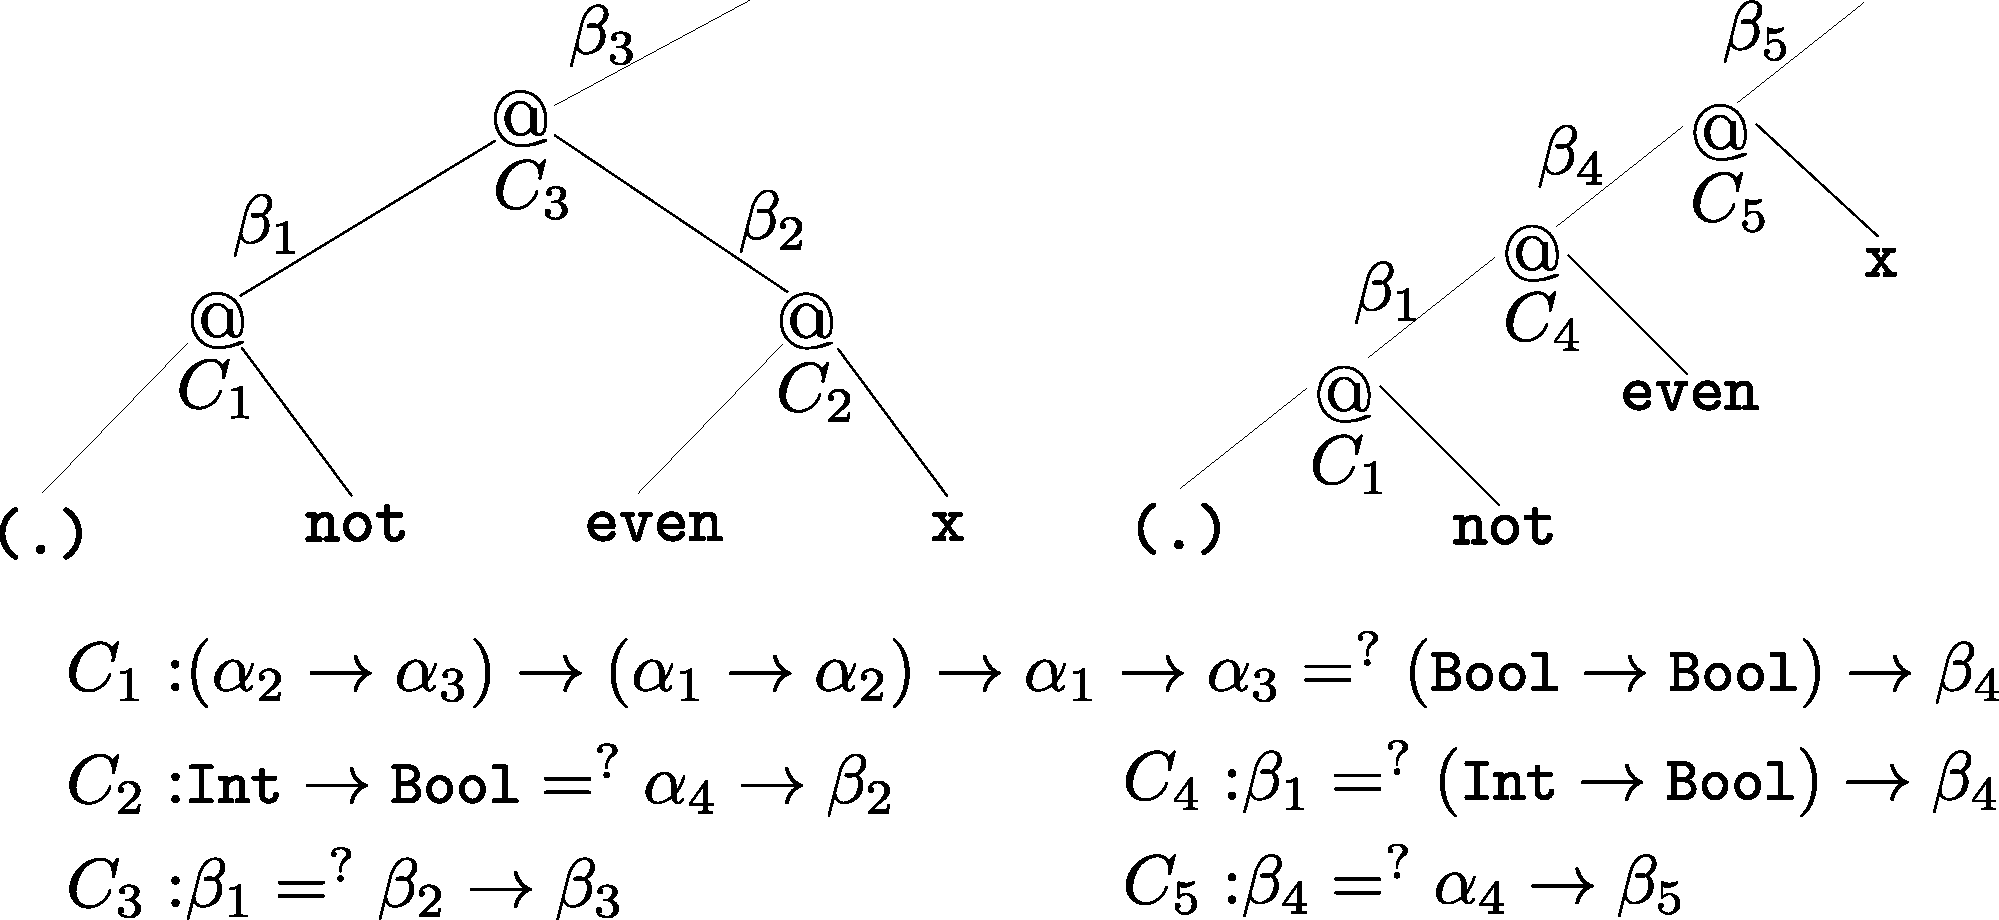
\includegraphics[width=0.85\columnwidth]{images/nonstruc.pdf}
\caption[Illustration of non-leaf type error.]{The ASTs and constraints for \prog{not . even x} (left)
and \prog{(not . even) x} (right).
\ensuremath{@}s denote function applications.
The parameter \prog{x} has the type $\tvf$.
Annotations on edges denote types for the corresponding
subexpressions. For example, $\tvvf$ is the type for the
subexpression \prog{ (.) not}.}
\label{fig:nonstruc}
\end{figure}

A precondition for
constraint-based methods to work well is that the
faulty constraint is included in the given set of
constraints. However, this precondition fails
for the type errors caused by missing pairs of parentheses
or brackets.
For example,
consider debugging the type error for \prog{odd}
introduced in Section~\ref{sec:background:leaves:search}.
The \cs\ for \prog{odd} includes three constraints,
as shown in the left of Figure~\ref{fig:nonstruc}, where it
also presents the program AST. The constraints and AST for the
expected correct definition of \prog{odd} are shown in
the right of Figure~\ref{fig:nonstruc}. From the figure,
we observe that no constraint in \cs\ could be identified
as the faulty constraint such that changing the corresponding
subexpression would bring \prog{odd} to the
well-typed version, and consequently constraint-based debugging
methods fail to locate the real error cause. In this example,
both \toolH\ and \toolS\ blame the subexpression \prog{even x}
as the error cause.

%
For other non-leaf type causes, such as extra pairs
of parentheses, the precondition also fails to hold,
which makes constraint-based approach not work well.
We give evidence of this
for Helium in Section~\ref{sec:causes}.
%
In addition, constraint-based methods don't work well when there are
multiple error causes. One reason is that most
error debuggers try to report type errors in as few locations
as possible. As a result, even if the real error cause contains
multiple leaves, the debugger may return an error cause with
fewer leaves. For example, while the real error cause for
\prog{vulOp1} includes both \prog{(<)} and \prog{"~"},
Helium~\cite{Heeren05:TQT} suggests that the error cause
is \prog{replicate}.

Overall, constraint-based methods don't work well when a type
error is non-structural or involves multiple leaves.

\subsection{When Type Annotations Are Correct}
\label{sec:background:annotations}

While type inference can recover most omitted
type annotations, it is considered as a good
practice to add type annotations to at least
top-level bindings\footnote{http://en.wikibooks.org/wiki/Haskell/Type\_basics\#Type\_signatures\_in\_code}
for many reasons. As a form of documentation, type annotations improve
program readability. Compilers often exploit type annotations
to make type inference more efficient.

Type annotations also help to increase error
locating precision. For example,
the function \prog{vulOp} is
actually well typed if we remove its type annotation,
and it is the type annotation that helps error debuggers to detect
the type error in it. For this reason,
all GHC, Helium~\cite{Heeren03:HLH,Heeren05:TQT},
and \toolMin~\cite{Pavlinovic14:FMT,Pavlinovic15:PST}
treat user-specified type annotations as hard
constraints, meaning that they should always be trusted.
Once there is some error in type annotations, the
generated error messages is misleading, and following the
message will lead to more type errors in the program.
Thus, error debuggers work well when type annotations
are correct.

\section{Study Subjects and Methodology}
\label{sec:subjects}


This section provides the study subjects and the methodology used to study the process of fixing type errors.
I first describe the study subjects used in this work in Section~\ref{sec:subjects:db}.
Section~\ref{sec:subject:ref} discusses how the correct programs for ill-typed programs are determined.
At last, the information recorded to represent the real error debugging is presented in Section~\ref{sec:subject:metric}.


\subsection{Analyzed Datasets}
\label{sec:subjects:db}

A main challenge in this study is choosing appropriate data sets
for investigation. Since our goal is to study how type errors
were fixed, we need the data set to contain not only well-typed
programs but also intermediate ill-typed programs. This
requirement rules out most program data sets that teachers may
have collected while teaching functional programming, including those
offered through Massive Open Online Courses. In this work, we
use three Haskell data sets for our study. Figure~\ref{fig:datasets}
presents an overview of them.
%
For each data set, we give its name, the year it was collected,
%the programming language of the data set, 
the number of
programs in the data set, 
%
the number of program sequences in the data set 
(a sequence is the list of all programs from the same
student working on a specific assignment or exercise),
%
the number of ill-typed programs that
we investigated in the data set, the size range of programs
measured in LOC (Lines Of Code), the number of students
who took the corresponding course, and
the compiler that students used to compile programs.
%we used to compile each data set
%in the last column.

\begin{figure}
\centering
\begin{tabular}{c | c c c c c c c}
Name &  Year     & No.\ progs & No.\ seqs & No.\ ill-typed   & Size  & No.\ students & Compiler\\
\hline
\benchf     & 2002  & 29,000 & 759 & 1,000 $\clubsuit$   & 2--190  & 119 & Helium \\
\benchs     & 2003  & 23,000 & 799 & 1,604       & 5--180 & 143 & Helium \\
\benchl & 2017   & 6,274 & 486   & 153 & 5--90 & 33  & GHC \\
\end{tabular}
\begin{center}
$\clubsuit$: The benchmark contains 2,000 ill-typed programs, and
we randomly analyzed 1,000 of them.
\end{center}
\caption{An overview of the data sets used for the study.}
\label{fig:datasets}
\end{figure}

The first two data sets were collected at Utrecht University,
and they included programs written
by first-year students learning the functional programming
language Haskell~\cite{jones2003haskell}, in years 2002 and 2003,
respectively. A copy of each program that
was compiled with Helium~\cite{Heeren03:HLH} and its
corresponding timestamp were recorded. These programs were written by
student to attempt to solve programming exercises or assignments, including
insertion sort,
string processing (such as calculating the maximum width of
strings in each column or padding each string in the table to
a certain length), boolean logic representations and operations, etc.
We defer detailed discussions about these program
sets to~\cite{Keeken06:AHP,Hage09:Neon}.

The data set \benchl\ was collected from an ongoing course. So far,
students in the course have worked on simple problems only, such as
representing binary values and converting them to decimal values,
computing Fibonacci sequences, determining whether lists are palindrome,
etc.

The ratio that the number of ill-typed programs
over the number of all programs
varies a lot across different data sets. In particular,
the ratio of ill-typed programs
%for \bencht\ is very high and that 
for \benchl\ is very low. 
This is because in this data set there is an
excessive number of well-typed programs that are similar,
which is potentially caused by 
the way how student
solutions are graded. The course uses an online
interface, where students submitted their solutions and received
feedback about whether their programs meet the assignment requirements immediately.
Usually students needs to finish an assignment by multiple steps,
and they can work on later steps only after passing the earlier steps.
Therefore, at each step students may keep on updating well-typed programs
until the running results of their programs are correct, yielding numerous
similar and well-typed programs.

For each data set, we used the compiler that was used in the class (last column in Figure~\ref{fig:datasets})
%
to compile each program,
collected the error messages for programs that have type
errors 
%but no unbound variables (since we can not decide what
%they were referring to), 
and analyzed the log file.
We did not consider programs that have unbound variables
because ignoring them does not affect our analysis results. 
We consider two cases when programs have unbound variables. 
In the fist case, 
%
the program do not contain any type error besides 
unbound variables. Such programs are irrelevant to 
our analysis. In the second case, the program does
contain type errors besides unbound variables. 
%
However, probably because Helium always reports 
unbound variable problems before reporting
type errors, students
always handled unbound variables first in such 
programs. Once the issue about unbound variables
was resolved, all type errors were exposed 
in the later versions of the student program, which we analyze.
Therefore, no information about type errors is missing
in our analysis. 

The program sets enable us to conduct our analyses 
at different scales.
To study how type errors were fixed,
we collected sufficient information 
by comparing each ill-typed program with its
corresponding student-intended well-typed program.
%which we call the \emph{reference program}. 
We discuss the
process of finding reference programs in detail in
Section~\ref{sec:subject:ref}.
%
To study what students did for fixing type errors,
we compared each ill-typed program with its next version of the program.
Moreover, by considering all the ill-typed programs over a period of several weeks,
we are able to study how the error fixing process evolved as students became more
familiar with the programming language.

\subsection{Finding the Reference Program}
\label{sec:subject:ref}

It is essential in our analysis procedure to choose,
for each ill-typed program,
a \emph{reference} program, which is the correct version of
the ill-typed program written by the same student.
Since identifying the reference program requires us to
understand the intention of the student
as well as the type error occurred in the program, it is impossible
to automate the procedure.
%just show that here we can use 'as a result' :)
As a result, we manually chose reference programs
to conduct the analysis on type error debugging.

%We discuss the process of how to choose the reference program in this subsection. 

%
%When a program contains multiple type errors,
%different type errors may be fixed in different references.
%different references may be
%used for fixing different type errors.



For each exercise finished by a student, we can
construct a \emph{program sequence},
including the student programs \pg{s}\ for the exercise,
the compiling results of \pg{s}, and the compiling time stamps.
%For simplicity, we use \seqijk\ to denote the
%program sequence for the exercise \pe.
%
%In manual analyses, we recorded various kinds of information
%to understand how type errors were fixed and what students did,
%detailed below.
%
Given a program sequence, denoted by \sseqijk,
we assume \pgi\ is ill typed, 
and \pgj\ is the first well-typed program after \pgi, 
and \pgk\ is another well-typed program after \pgj.
We follow the rule containing three cases below to
identify the reference program for \pgi\ in
the program sequence.
Without losing generality, we first illustrate the rule
by assuming that there is only one type error in \pgi.
After that, we show how to apply the rule to
find reference programs when \pgi\ has multiple errors.

%To identify the reference program of \pgi\ in the program sequence,
%we can follow the three steps below
%there are in general three different cases,
%and we present more likely case first as follows.

\paragraph{Case 1: \pgj\ is the reference for \pgi}
This is the most simple and straightforward case, 
where there is no intermediate well-typed program between 
\pgi\ and \pgj, and the programs after \pgj\ are not about 
fixing the type error in \pgi.
Take the student program sequence below as an example.\footnote{The original function had the Dutch name \prog{uitVullen}. To improve
readability, we have translated all Dutch names to English, except
for those we do not know how to translate or translation leads to name conflicts.}
The program is to make the string
\prog{s} up to a length of \prog{i} by
padding \progsq{\,}s.
%append a list of \prog{' '} at the end of a string.
We added the group and time information,
as well as the program name to the excerpt of each program in italics.
%
\begin{program}
fillOut :: String -> Int -> String \hfill \it{group103/2004-01-10@14_49_38_273 \quad p\textsubscript{1}}
fillOut s i = replicate (i - (length s)) " "

fillOut :: String -> Int -> String \hfill \it{group103/2004-01-10@14_50_10_811 \quad p\textsubscript{2}}
fillOut s i = replicate (i - (length s)) ' '

fillOut :: String -> Int -> String \hfill \it{group103/2004-01-10@15_51_33_552 \quad p\textsubscript{16}}
fillOut s i = s ++ (replicate (i - (length s)) ' ')
\end{program}
%
Both $\it{p\textsubscript{2}}$ and $\it{p\textsubscript{16}}$ are well typed, 
and $\it{p\textsubscript{16}}$ is the submitted version of the student program.
Based on the program sequence, we say
$\it{p\textsubscript{2}}$ is the reference of $\it{p\textsubscript{1}}$
because $\it{p\textsubscript{2}}$ is well typed,
and the changes after $\it{p\textsubscript{2}}$ are irrelevant to
the type error in $\it{p\textsubscript{1}}$,
and the final program $\it{p\textsubscript{16}}$ contains $\it{p\textsubscript{2}}$.

\paragraph{Case 2: \pgk\ is the reference for \pgi}
In this case, there exists the intermediate well-typed program \pgj\ 
between \pgi\ and \pgk, 
%\pgk\ is well typed, 
and the programs after the well-typed \pgk\ is not about fixing the type error in \pgi.
%
%In the second case, \pgk\ is the reference of \pgi, and \pgj\ is
%the intermediate well-typed program between \pgi\ and \pgk.
For example, \pgj\ might eliminate the type error
in \pgi\ by removing part of its ill-typed expression, and later
\pgj\ is changed into \pgk\ to have the expected functionality.
The type error in \pgi\ is relevant to the edits in \pgk,
while it is irrelevant to the further changes after \pgk.
Note that it is possible that there are multiple
intermediate well-typed programs
between \pgi\ and \pgk\ in a real program sequence.

%To better illustrate the second case, we use the following
%sequence from the program database as an example.
Consider the following sequence from the program database,
where 
\prog{Table} is defined as \prog{[[String]]} (In the whole
paper, \prog{Table} is a type synonym for \prog{[[String]]})
and \prog{widthColumn} is defined in the same program
and has the type \prog{Table -> [[Int]]}.
%
The function \prog{widthColumn} uses a matrix to store the length of 
every string in a \prog{Table},
and the function \prog{largestWidth} tries to compute the maximum
length of the string in each column of a \prog{Table}.
%We added the group and time information as well as the program
%name to the excerpt of each program in italics,
%and 
We omitted all the ill-typed programs between \pga\ and \pgc.
%
%and we use \prog{grootsteBreedte} as a short name for \prog{grootsteBreedte} in the original program.
%
\begin{program}
largestWidth :: Table -> [[Int]]  \hfill \it{group7/2005-01-10@12_36_57_499 \quad p\textsubscript{1}}
largestWidth t@(x:xs) = map maximum (transpose (widthColumn t))

largestWidth :: Table -> [[Int]] \hfill \it{group7/2005-01-10@12_37_33_561 \quad p\textsubscript{3}}
largestWidth t@(x:xs) = transpose (widthColumn t)

largestWidth :: Table -> [Int] \hfill \it{group7/2005-01-10@12_39_22_178 \quad p\textsubscript{6}}
largestWidth t  = map maximum (transpose (widthColumn t))
\end{program}
%
%\begin{program}
%\textit{group7/2005-01-10@12_36_57_499 \hfill p\textsubscript{1}}
%largestWidth :: Table -> [[Int]]
%largestWidth t@(x:xs) = map maximum (transpose (widthColumn t))
%
%\textit{group7/2005-01-10@12_37_33_561 \hfill p\textsubscript{3}}
%largestWidth :: Table -> [[Int]]
%largestWidth t@(x:xs) = transpose (widthColumn t)
%
%\textit{group7/2005-01-10@12_39_22_178 \hfill p\textsubscript{6}}
%largestWidth :: Table -> [Int]
%largestWidth t  = map maximum (transpose (widthColumn t))
%\end{program}
%\noindent
By removing the functions \prog{map} and \prog{maximum},
\pgb\ removes the type error in \pga. However,
\pgc\ is the correct reference program of \pga.
This is because no later changes after \pgc\ is relevant
to the type error in \pga, and
\pgc\ matches the student's intention according to
his/her final submitted program.

\paragraph{Case 3: no reference for \pgi}
%
We fail to find the reference program 
if the well-typed programs like \pgj\ or \pgk\
are not about fixing the type error in \pgi,
or if there is no well-typed program in the sequence.
There are two reasons that the reference does not exist in a program sequence.
First, the student gave up
fixing the type error and rewrote the whole code.
Second, the student switched to other compilers in later
versions~\cite{Keeken06:AHP} since using Helium was not mandatory.
We ignored such program sequences with no references since we are
not able to know students' intentions for them.
In our analysis, there are about 6\% of ill-typed programs
in the database we can not find their reference programs.

%strat to describe how the rule works for multiple errors with an example
%Considering an ill-typed program could contain more than one type error in practice,
%the way of finding program reference should be type-error based.
%
We now turn to the situation that a program may contain multiple
type errors. 
We use the following edit sequence of the program
\prog{printTable} to illustrate 
how the rule described above works to find reference programs
in this situation.
%when there are multiple type errors in a program.
%
%\begin{program}
%printTable :: Table -> String
%printTable (x:xs)   = printTableHeader x:xs ++ printTableContent tail (x:xs)
%\end{program}
%
\begin{program}
printTable :: Table -> String \hfill \it{group7/2004-02-02@11_28_36_363 \quad p\textsubscript{1}}
printTable (x:xs) = printTableHeader x:xs ++ printTableContent tail (x:xs)

printTable :: Table -> String \hfill \it{group7/2004-02-02@11_29_37_477 \quad p\textsubscript{2}}
printTable (x:xs) = printTableHeader x:xs ++ printTableContent (tail (x:xs))

printTable :: Table -> String \hfill \it{group7/2004-02-02@11_33_41_536 \quad p\textsubscript{7}}
printTable (x:xs) = printTableHeader x:xs

printTable :: Table -> String \hfill \it{group7/2004-02-02@11_40_16_149 \quad p\textsubscript{12}}
printTable (x:xs) = printTableHeader x

printTable :: Table -> String \hfill \it{group7/2004-02-02@11_43_52_864 \quad p\textsubscript{14}}
printTable (x:xs) = printTableHeader x ++ printTableContent (tail (x:xs))
\end{program}
%
%\begin{program}
%printTable :: Table -> String \hfill \it{group7/2004-02-02@11_28_36_363 \quad p\textsubscript{1}}
%printTable (x:xs) = printTableHeader x:xs ++ printTableContent tail (x:xs)
%
%printTable (x:xs) = printTableHeader x:xs ++ printTableContent (tail (x:xs)) \hfill \it{p\textsubscript{2}}
%
%printTable (x:xs) = printTableHeader x:xs \hfill \it{p\textsubscript{7}}
%
%printTable (x:xs) = printTableHeader x \hfill \it{p\textsubscript{12}}
%
%printTable (x:xs) = printTableHeader x ++ printTableContent (tail (x:xs)) \hfill \it{p\textsubscript{14}}
%\end{program}
%
In the program, \prog{printTableHeader} has the type \prog{Row -> String}, where \prog{Row} is defined as \prog{[String]}.
It intersperses all the strings in a row with
\progsq{+}s and concatenates them.  
%
The function \prog{printTableContent} has the type \prog{Table -> String},
and it intersperses all strings in a \prog{Table} with \progsq{|}
and concatenates them.
%
The function \prog{printTable} tries to append the results of \prog{printTableHeader} and \prog{printTableContent} together.
%
%

There are two type errors in the first program
$p\textsubscript{1}$, as can be seen by comparing it
with the final 
well typed program $p\textsubscript{14}$.
%
%We list the program sequence of \prog{printTable} as follows,
%and we show how to find the corresponding reference of each error.
%In the sequence, $p\textsubscript{12}$ is the intermediate well-typed program,
%and $p\textsubscript{14}$ is the final well-typed program.
%For simplicity, we omitted some unimportant steps in the sequence.
%
%
The second type error in the original program is removed in $p\textsubscript{2}$,
and the programs after $p\textsubscript{2}$ do not contain any changes 
related to \prog{printTableContent (tail (x:xs))}.
Therefore, $p\textsubscript{2}$ is the reference of the second error,
although the program itself is not well typed.
%
%
After the second type error is removed in 
$p\textsubscript{1}$, we can apply \textit{Case 1} above
to $p\textsubscript{1}$ to determine $p\textsubscript{12}$
as the reference 
for the first type
error in \prog{printTable}.
% is the last program $p\textsubscript{12}$. 
%The first type error is removed in 
%According to the rule, the reference of the first type error in 
%$p\textsubscript{1}$
%%the original program
%is $p\textsubscript{12}$.
%%
%Note that $p\textsubscript{12}$ is well-typed, 
%and it keeps the same in the student's submitted program $p\textsubscript{14}$.

Different errors in the same program may have different references.
Consequently, we study how each type error was fixed by investigating
the changes made, with respect to the error, between the original program
and the reference. We show more details about how the changes are measured
for each type error in the next subsection.

\subsection{Analysis Metrics}
\label{sec:subject:metric}

We constructed two records,
namely \emph{final fix} and \emph{fixing process},
for the analysis of how type errors were fixed and what students did, respectively.
Assume \pgi\ is the ill-typed program in \seqij, and \pgj\
is the reference of \pgi.
For the final fix record, we compare each \pgk\ with \pgj, where $k \in [i,j)$, 
and record the related information.
For the fixing process record, we compare each \pgk\ with $\pg_{k+1}$,
where $k \in [i,j)$, and record the related information.
In this subsection, we propose five metrics that
are used to represent the information in both records.

Before presenting the metrics,
it is important to note that a single metric may have
different meanings in different records.
Take the number of leaves changed in ASTs as an example.
In the final fix record, this metric reflects how
a program should
be changed to remove type errors.
%
In contrast, in the fixing
process record, it indicates what students did in
response to type errors.
Thus, the final fix record shows how type error debugging
looks like in practice while the fixing process record
reveals students' preferences and behaviors for fixing
type errors.


Next, we explain each metric used and how we measure it.
We use the following example \prog{maxLengte} to illustrate our calculations.
From this program on, we present the reference program in italics below the ill-typed program.
%
\begin{program}
maxLength :: [String] -> Int
maxLength x = maximum (map (length x))
\it{maxLength x = maximum (map length x)}
\end{program}
%
The error message generated by Helium is:
%
\begin{program}
(41,24): Type error in application
 expression       : map (length x)
 term             : map
   type           : (a -> b) -> [a] -> [b]
   does not match : Int      -> [Int]     
 because          : not enough arguments are given
\end{program}


Besides the reference program, number of fixing steps, 
and the creation date,
the measurements of the following metrics are recorded for each error.
Note that we focus on the place where
student changed to fix the type error.
%the changes made by students are directly
%related to the type error.
For example, in the program \prog{printTable}, although the student changed
the function \prog{printTableHeader} (called
by the function \prog{printTable}) 
during the debugging process,
we do not consider the 
leaf changes in it.


\begin{itemize}[noitemsep]

\item \textbf{Non-leaf/Leaf change}.
This metric represents whether the error cause is non-leaf or in leaves.
If it is non-leaf, we record the numbers of pairs of parentheses and
brackets that are added and
removed, respectively. 
Otherwise,
we record the number of leaves that are changed in program ASTs.
In the \prog{maxLength} example, for the
final fix record,
only one pair of parentheses was
removed,
and consequently it is Non-leaf change.


\item  \textbf{Correctness of type annotations}.
This metric reflects the reliability of type annotations in student programs.
We measure it by checking if the type annotation in the current program
is the same as the one in the reference.
In the \prog{maxLength} example, the type annotation is correct.
%This allows us to study the reliability of type annotations in type error debugging.

%\item The number of type errors in each ill-typed program.
%By recording how the number of type errors changes during the fixing process,
%we are able to discover the behaviours of students for dealing with multiple type errors.

\item \textbf{Size difference}.
This metric is the sum of the size of the expression
that is changed from in the original program
and
that of the expression that is 
changed to in the reference program. 
We use the notation $n$--$m$ to denote that
$n$ nodes and $m$ leaves in the AST are changed.
This metric measures how close the two
expressions are: the larger is this value, the more efforts are needed to
make the change.
In the \prog{maxLength} example, 
the expression changed from is
\prog{map (length x)} and that changed to is \prog{map length x}.
Their sizes are 3--2 and 3--2, respectively.
Therefore, the size difference is 6--4.
%Similarly, the size difference for the second error is 14--8.
% based on the modified program excerpt \prog{tail (x:xs)}.
%By observing this information over multiple steps in the program sequence,
%we can decide if ill-typed programs are increasingly close to their
%references or there is a diverging phase in fixing process.

\item \textbf{Helium information}.
For this metric, we consider:
\begin{enumerate*}[label=(\alph*)]
\item does Helium locate the real error cause correctly,
\item whether following Helium's change suggestion will bring
the current program to the reference program,
\item the distance between the real error cause and the one reported
by Helium in terms of the number of identifiers, and
\item the category of the change suggestion.
\end{enumerate*}
%
We extract these items by investigating the current program,
the reference program, and the Helium error message for the corresponding error.
For example, the results for items (a), (b), and (c)
in \prog{maxLength} are ``no'', ``no'', and 1, respectively. 
We discuss item (d) in detail in Section~\ref{sec:effectiveness}.
%
The purpose of this metric is not to evaluate the quality
of error messages of Helium, but rather to study how
the precision of error locating and different message categories 
affect the error debugging in practice.
%\item Number of intermediate correct programs.
%We count the number of correct programs
%between the ill-typed program and the reference program.
%This, together with some other information about
%the corresponding correct programs like the changes of expression sizes,
%allows us to investigate how students work toward the well-typed programs.

%\item Whether the expression is the same as before.

\item \textbf{Difficulty reason}.
Debugging difficult type errors usually takes
students more steps or more time.
We summarize the difficulties based on different aspects of language features,
namely \emph{type annotations},
\emph{library function usage}, \emph{function composition},
\emph{point-free function}, and \emph{pattern matching}. 
We discuss more details of the difficulty reasons in
Section~\ref{sec:difficulty}.
This metric
allows us to discover which language features are difficult to students
with respect to type error debugging.
For example, the student took 9 steps to fix the type error in \prog{maxLength},
and the difficulty is due to the wrong function composition of \prog{map} and \prog{length x}.

\end{itemize}


\noindent
For final fix, all these metrics are used in the work. For
fixing process, only the metric Non-leaf/Leaf change is used
in Section~\ref{sec:causes}.


\chapter{Debugging Behavior Analysis}
\label{sec:analysis}

This chapter presents the analysis results based on the three datasets introduced in Section~\ref{sec:subjects:db}.
A bird's-eye view of the findings about students' debugging process is first provided in Section~\ref{sec:overview}.
Then, I present the statistical results of error locations (Section~\ref{sec:causes}), type annotation reliability (Section~\ref{sec:annotation}),
error message effectiveness (Section~\ref{sec:effectiveness}), and difficult language features (Section~\ref{sec:difficulty}) in the respective section. 
At last, I discuss the threats to validity in Section~\ref{sec:threat}.

\section{Overview of Error Debugging in Practice}
\label{sec:overview}

\begin{figure}
\centering
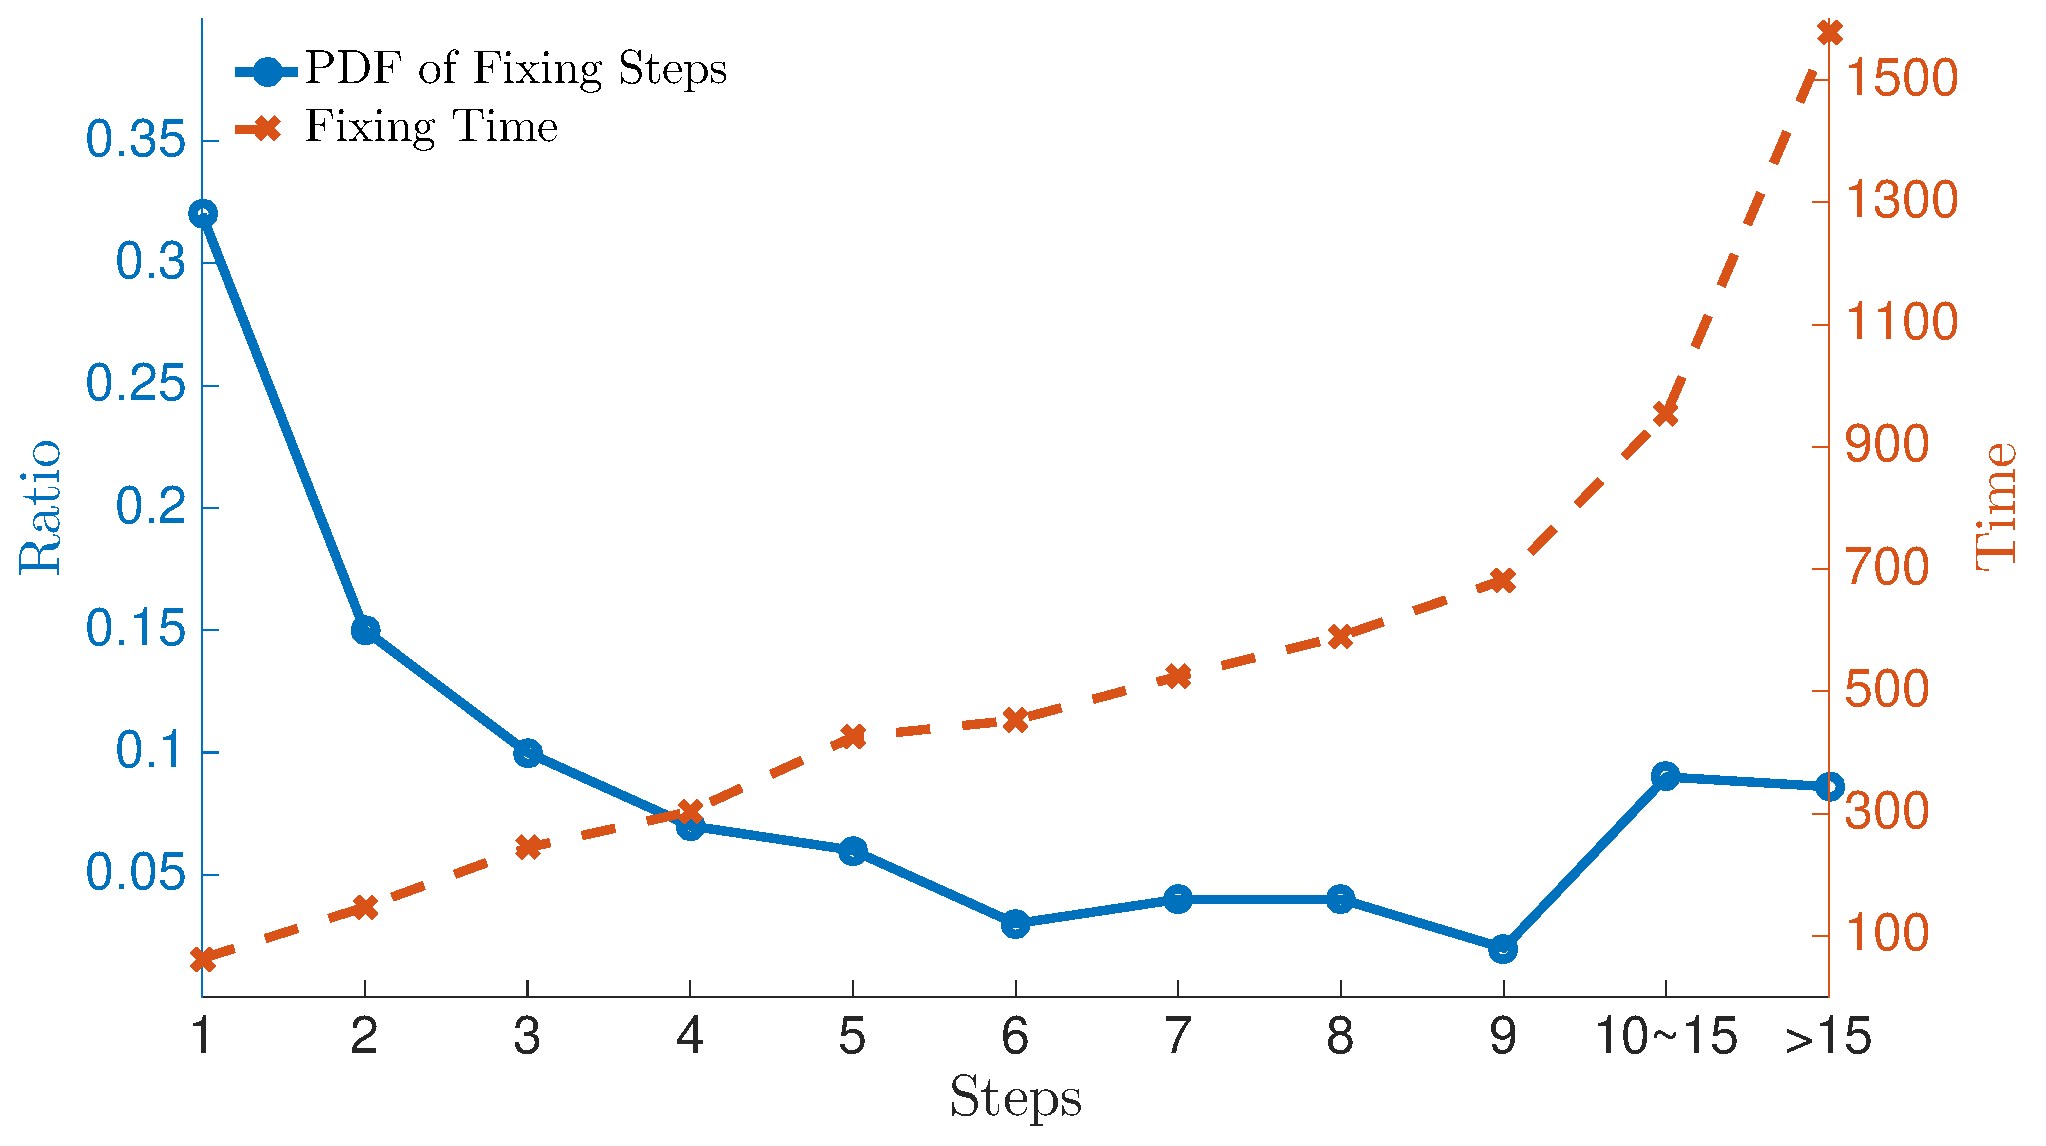
\includegraphics[width=.85\columnwidth]{images/step_time.eps}
\caption{Fixing steps and times in program data sets}
\label{fig:fst}
\label{fig:overview:overview}
\end{figure}

In this section, we present an overview about the number
of steps and time duration students spent on fixing
type errors by considering the three data sets
together. We also show how they evolve over an eight-week
period. 
%
Figure~\ref{fig:fst} shows the distribution of 
fixing steps, where any point $(x,y)$ on the 
solid curve denotes that the ratio of type errors
fixed with $x$ steps over all the type errors is
$y$. 
%
%
For example, (1,32\%) indicates that 32\% of all type
errors are fixed within a single step. 
%There are 32\% of the errors fixed by one steps, 
%which is the most common case in debugging situations.
%
The ratio decreases as the number of fixing steps increases.
%
While many type errors are fixed within a couple of 
steps (probably due to some obvious mistakes that are easy
to fix), 
a large portion of type errors required
more steps to fix.
For example, about 30\% of the errors took more than 5 steps to fix,
and 18\% of the errors took more than 10 steps to fix.
In average, the number of fixing steps 
is 4.7 (\std \footnote{\std\ is the standard deviation}=6.2)
for \benchf,
5.8 (\std=8.0) for \benchs, 
and 4.3 (\std=5.1) for \benchl.
Here we have large standard deviations because 
the data sets contain large variations of error fixing
situations. For example, many type errors were fixed with
just 1 or 2 steps while others might take more than 15 steps.


Figure~\ref{fig:fst} also shows the relation 
between time duration and the number of fixing steps.
To increase the readability, we show only the average
time for each number of fixing steps in the figure. 
%
In general, the time increases as the number 
of fixing steps increases. 
For example, students spent 63 seconds on average
for errors that are fixed with a single step,
425 seconds for errors fixed with 5 steps,
and 842 seconds for those fixed with 10 steps. 
%
The correlation coefficient between 
fixing time and the number of fixing steps
is 0.81 with the \emph{p}-value $< 1e^{-13}$ (
the correlation coefficient is computed 
based on all fixing duration with respect to fixing steps).
As the correlation is strong,
we can either use the number of fixing steps
or fixing time to reflect the difficulty of error debugging  in our later discussions.


\begin{figure}
\centering
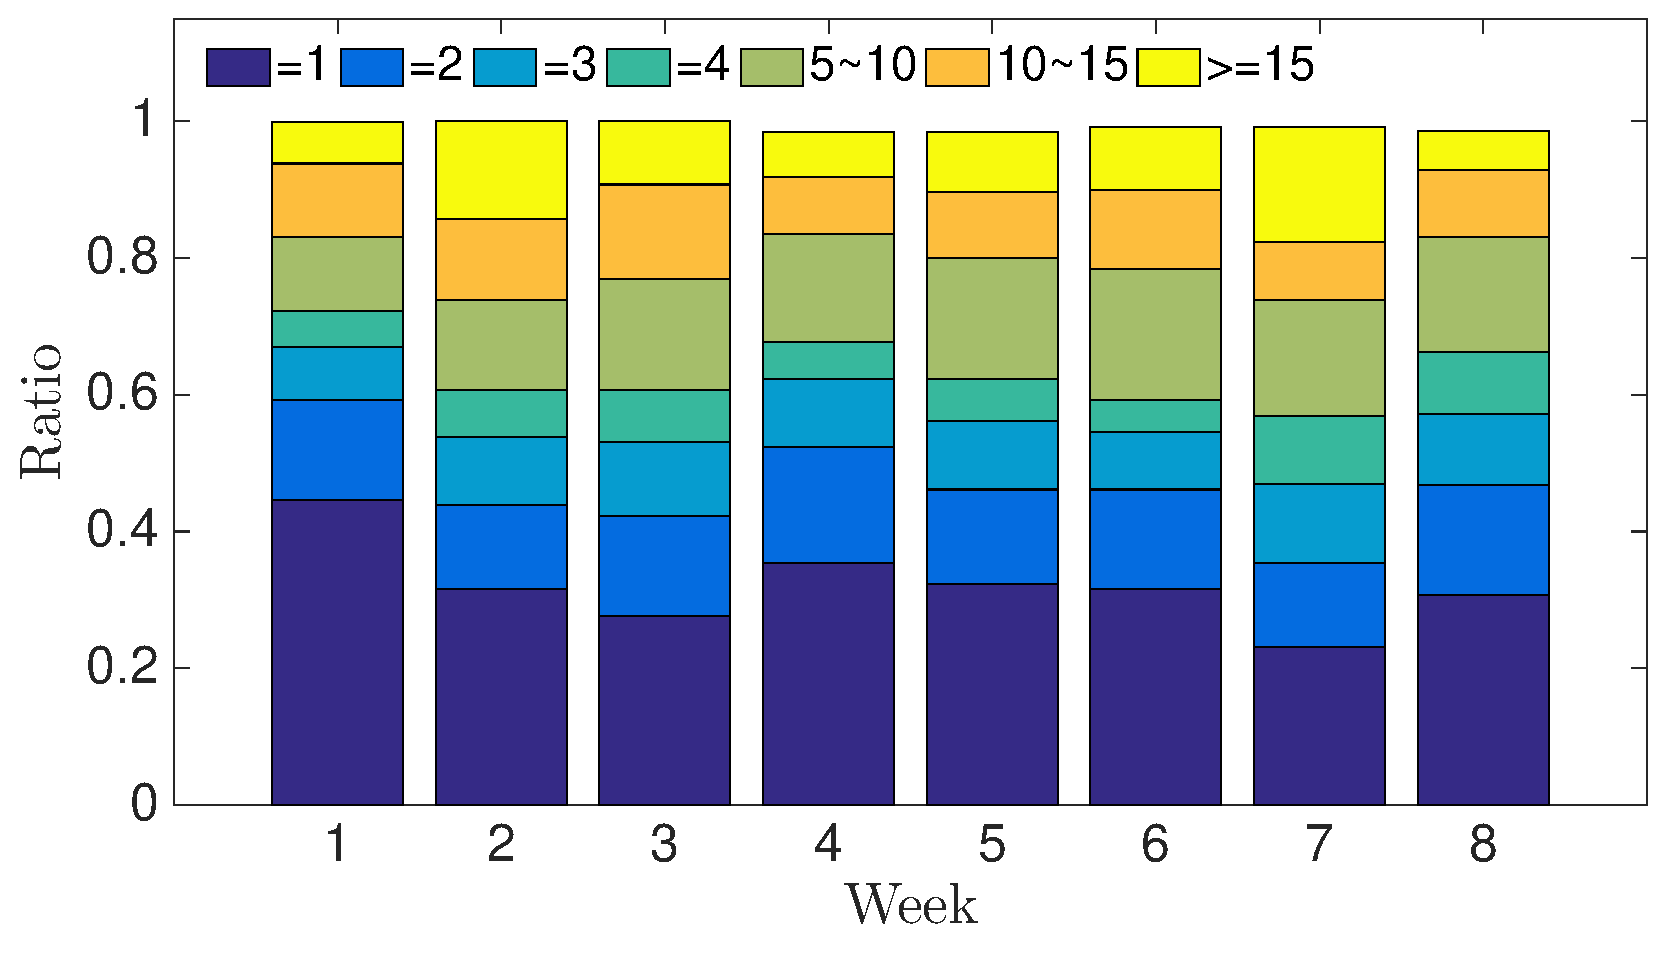
\includegraphics[width=0.85\columnwidth]{images/step_time_ratio_1.eps}
\caption{Distribution of fixing steps over the time}
\label{fig:sot}
\label{fig:overview:dos}
\end{figure}


Figure~\ref{fig:overview:overview} shows that the numbers
of fixing steps vary a lot. We are also interested in knowing
if this variability was preserved over time.
Specifically we want to know 
if students tended to have longer error
debugging sequences when they first started to learn the language
while have shorter 
sequences as they became more experienced 
with the language
and type error debugging.
%
%it does not tell whether
%time points (such as the first or last week) are relevant.
%
Figure~\ref{fig:sot} 
addresses this question
by showing 
the evolution of the numbers of fixing steps
over an eight-week period.
The figure considers \benchf\ and \benchs\ together.
For each week, we compute the ratio for each number
of fixing steps. 
%different fixing steps (e.g. step=1 or 5$\leq$step$<$10) in each week.
For example, the ratios of one-step fixes
range from 0.25 to 0.44 during week 1 to 8,
and the average ratio is 0.32 (\std=0.06). 
The value of \std\ is small, meaning that
one-step ratios do not change much over the time.
We have similar results about \std\ for other numbers of 
fixing steps. 
%
Therefore, the distribution of
different numbers of fixing steps is quite stable as time went by.


\cite{hage2006mining} shows
that the number of type errors students made in most
weeks are similar (except that
week one had fewer and week three had more
type errors). Together with the result in
Figure~\ref{fig:overview:dos}, we can conclude
that, type error debugging was consistently 
challenging over time for students, even after they
had been programming in Haskell, reading error messages,
and fixing type errors for several weeks. 

\section{Where Were Error Causes?}
\label{sec:causes}

In Section~\ref{sec:background:leaves}, we discussed that most error debuggers work well
when type errors are caused by single leaves.
In this section, we investigate how programs were fixed
by grouping all programs according to the number of leaves that
were changed. We write $n$-leaf to mean that $n$ leaves
were changed and write non-leaf to mean that
pairs of parentheses or brackets were added or removed. Our discussion assumes
that each program contains one type error only.
When a program contained multiple errors, we considered the type errors
individually.

\begin{figure}
    \centering
    \begin{subfigure}[t]{0.85\textwidth}
        \centering
        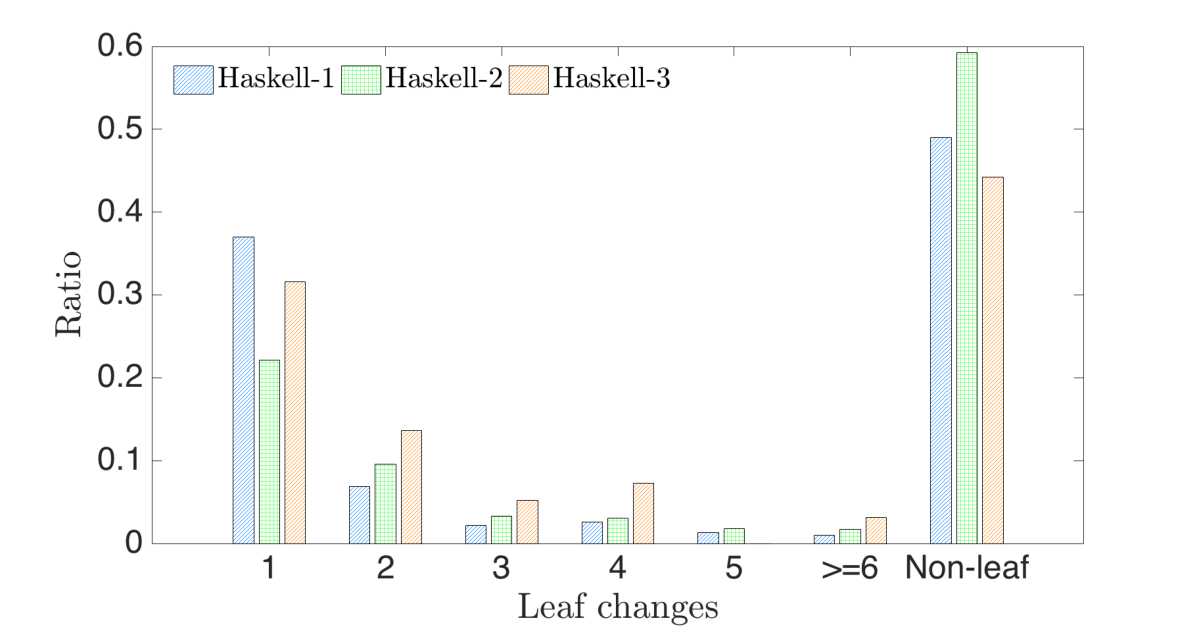
\includegraphics[width=0.95\columnwidth]{images/leaf-final.pdf}
        \caption{Distribution of leaf changes in final fix}
        \label{fig:leaf-chg-dist:final}
    \end{subfigure}
    
    \begin{subfigure}[t]{0.85\textwidth}
        \centering
        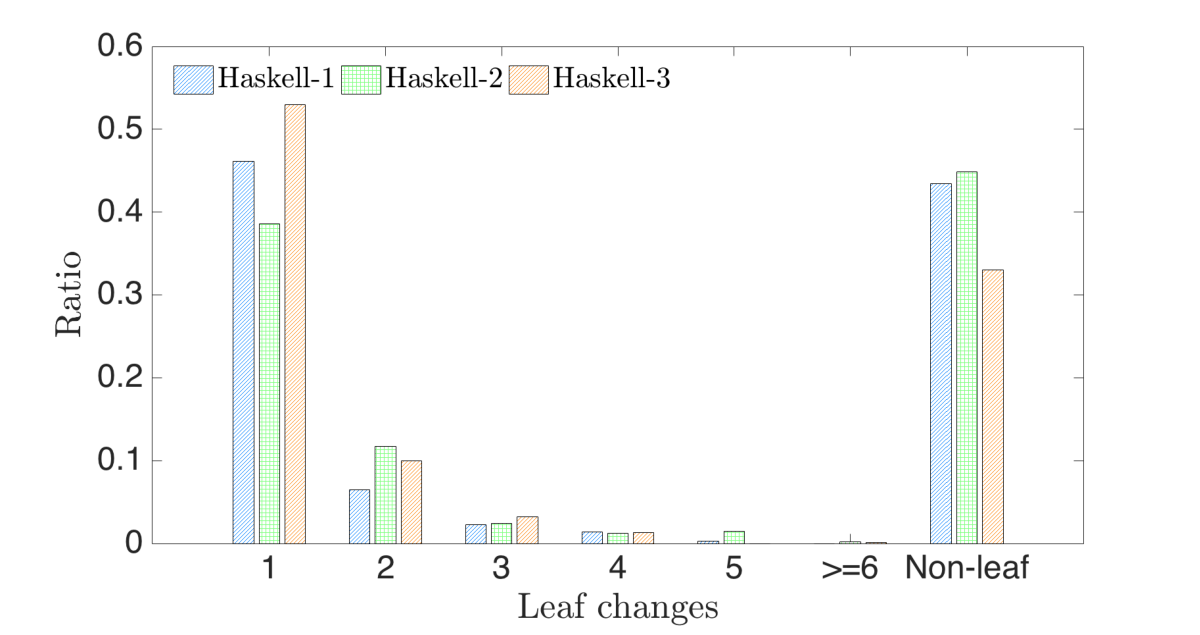
\includegraphics[width=0.95\columnwidth]{images/leaf-process.pdf}
        \caption{Distribution of leaf changes in fixing process}
        \label{fig:leaf-chg-dist:proc}
    \end{subfigure}%
    \caption{Distribution of leaf changes}
    \label{fig:leaf-chg-dist}
\end{figure}

Figure~\ref{fig:leaf-chg-dist} shows the distribution of
programs with respect to the number
of changed leaves in both the final
fix (Figure~\ref{fig:leaf-chg-dist:final})
and fixing process
(Figure~\ref{fig:leaf-chg-dist:proc}) records.
%
The ratio for $n$-leaf is calculated by dividing the number of
programs that belong to $n$-leaf over the number of all
ill-typed programs.
%
As we can see from Figure~\ref{fig:leaf-chg-dist:final},
non-leaf changes always account for the majority
of all kinds of leaf changes across different data sets. 
Specifically, the ratio of non-leaf change in \benchs\
reaches more than 50\%,
and the ratios are more than 45\% in the other two data sets.
In other words, more than
45\% of type errors were fixed
by adding or removing pairs of parentheses or brackets
in all data sets.
%
In contrast, for 1-leaf change, where existing debuggers work
well, its ratio ranges from only about 22\% in \benchs\ to about 37\%
in \benchf.

%
%
Figure~\ref{fig:leaf-chg-dist:proc} shows where students preferred
to make changes when fixing type errors. An interesting observation
is that, across all data sets, students made changes with respect to single leaves  
more often than non-leaf changes during fixing process. 
For example,
students made 1-leaf changes for about 39\% of all errors in \benchs,
while only about 21\% of changes were non-leaf.
Moreover,
the ratio of non-leaf changes is decreased from fixing
process to final fix in all data sets. For example, for \benchs,
the ratio is decreased from 60\% to 45\%.
%
These numbers imply that
either students were unaware of the high frequency of causing type
errors by wrong pairs of parentheses or brackets,
or they were misled by the error messages when type errors were non-leaf.
%
Consider, for example, the program \prog{maxLength} introduced in Section~\ref{sec:subject:metric}.
We can observe that actually the student got all the necessary identifiers (\prog{map},
\prog{length}, and \prog{x}) right but had an extra pair of
parentheses.
Unfortunately, the error message pointed to a wrong direction,
making the student take 9 steps to identify the real error cause.
This example shows that error debuggers fail to
convey information accurately
when type errors are not at leaves.

\begin{figure}
\centering
    \begin{subfigure}[t]{0.85\textwidth}
        \centering
        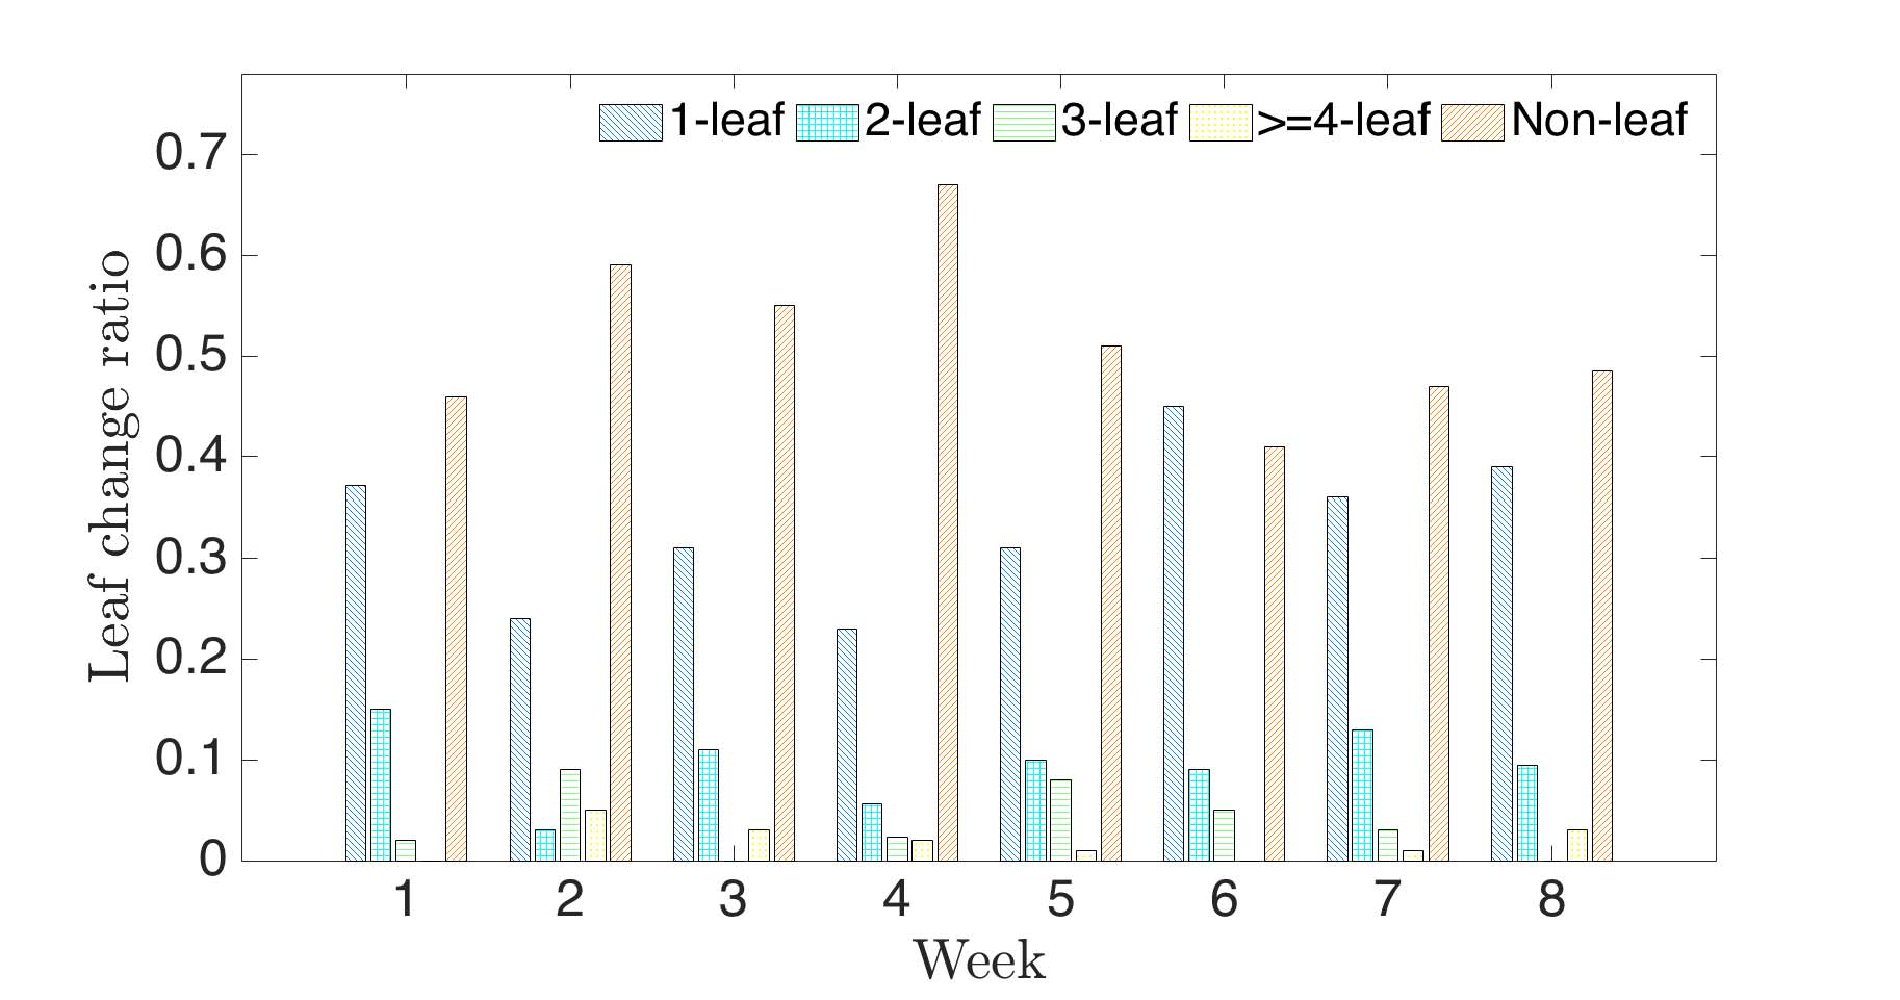
\includegraphics[width=0.95\columnwidth]{images/lt02.pdf}
        \caption{Evolution of leaf changes for \benchf}
        \label{fig:leaf-chg-evol:data1}
    \end{subfigure}%
    
    \begin{subfigure}[t]{0.85\textwidth}
        \centering
        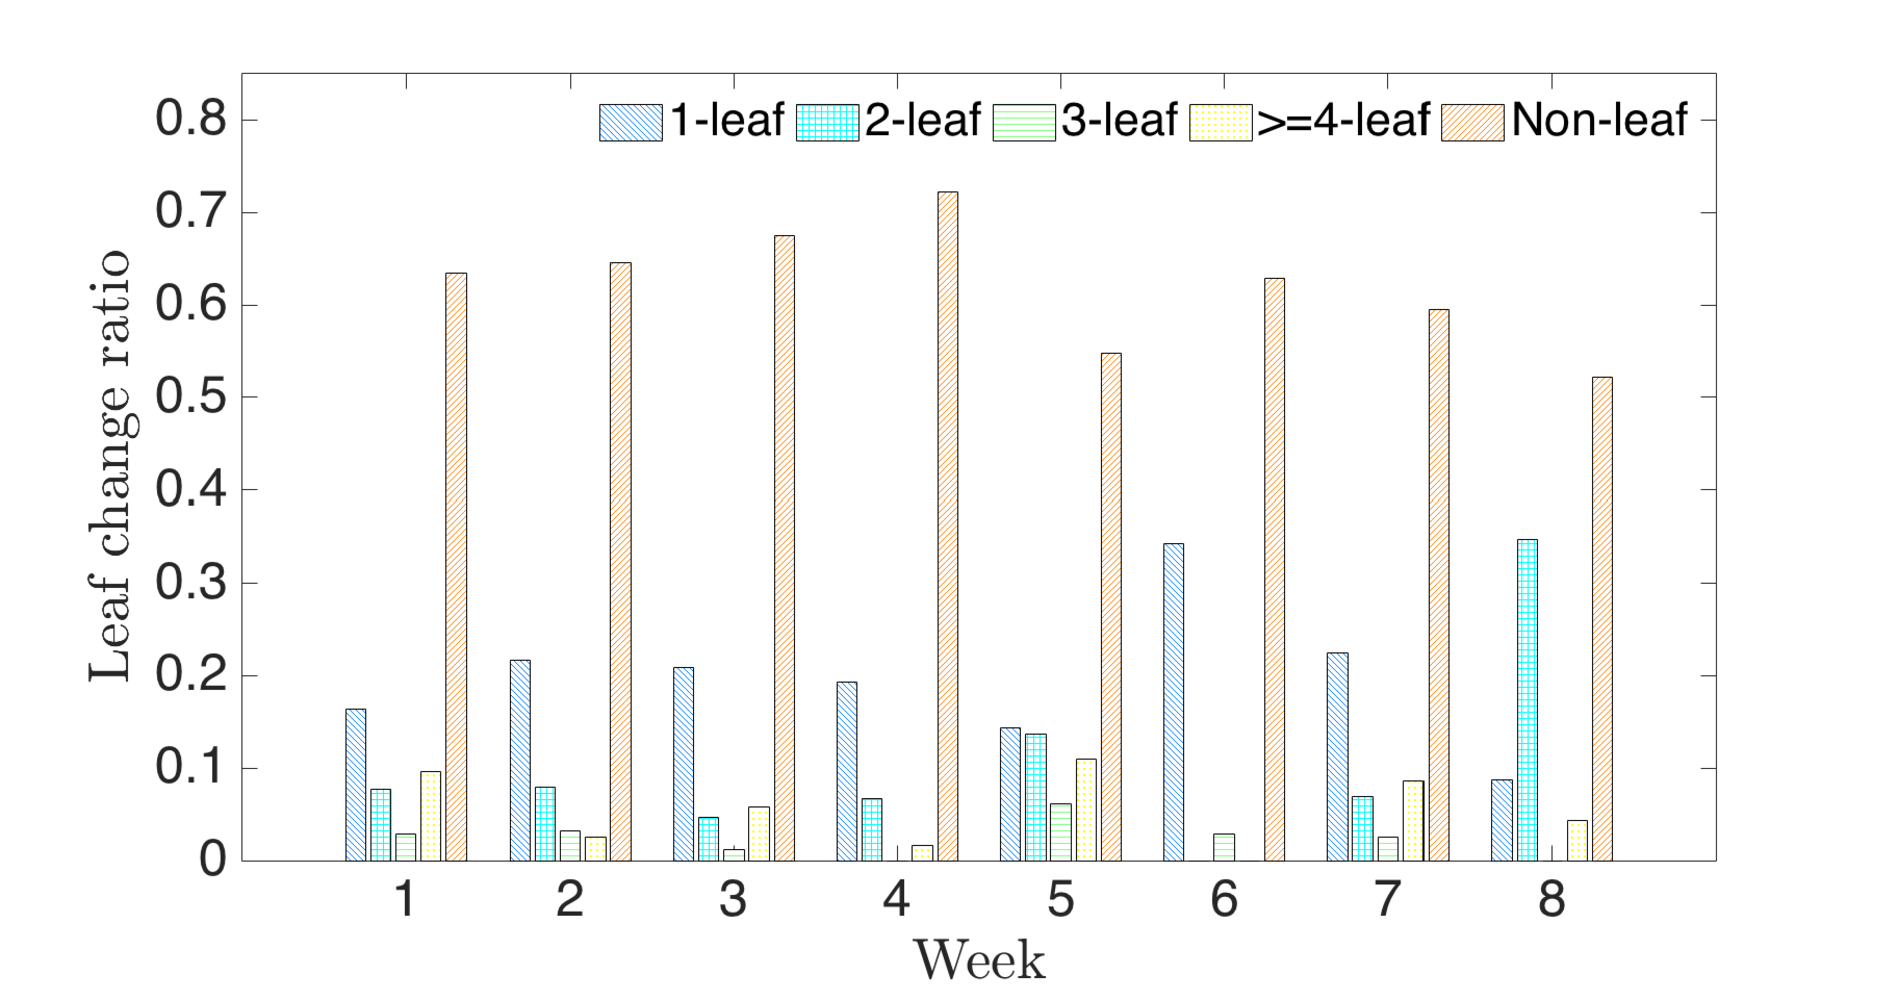
\includegraphics[width=0.95\columnwidth]{images/lt.pdf}
        \caption{Evolution of leaf changes for \benchs}
        \label{fig:leaf-chg-evol:data2}
    \end{subfigure}

    \caption{Evolution of leaf changes against weeks}
    \label{fig:leaf-chg-evol}
\end{figure}

Figure~\ref{fig:leaf-chg-evol} shows the evolution
of the ratios 
%of different kinds 
of leaf changes in the
final fix record. 
Note that week 1 denotes the
first week students submitted programs, not necessarily the
first week in the corresponding semester.
%In Figure~\ref{fig:leaf-chg-evol:data3}, we skipped the weeks
%that students had no submission in them. Also
We don't have such an evolution figure for \benchl\ because the
course is still ongoing and we had data for only 3 weeks.
%
%In particular,
%in all but only one week across all data sets, type errors were fixed
%more often by adding or removing parentheses than by changing
%single leaves. 
We observe that the ratio of non-leaf changes
ranges from 50\% to 70\%
while the ratios of 1-leaf change are always less than 40\% in \benchs.
For \benchf, we have a similar observation that the ratio of non-leaf changes is higher
than that of 1-leaf changes in most weeks. 
These figures again show that
most of the errors were not caused by single leaves in ASTs,
although the ratios vary from week to week.
Combined with our discussion in Section~\ref{sec:background:leaves},
the results in Figures~\ref{fig:leaf-chg-dist} and~\ref{fig:leaf-chg-evol}
indicate that most existing error debuggers may not work well in
real debugging situations.
%at least they are not able to locate type errors accurately in the student programs.


Figure~\ref{fig:lst} shows 
%how the number of fixing steps changes with
%different kinds of leaf changes.
the relation between the number of leaves changed and the number of steps to fix the type error.
%
Not surprisingly, the median value of the number of
fixing steps increases as more leaves are changed
in final fix.
The correlation values between fixing steps and leaf changes
in \benchf, \benchs, and \benchl\ are 0.423 (\emph{p}-value=$13e^{-15}$),
0.518 (\emph{p}-value=$1e^{-15}$), and 0.451(\emph{p}-value=$1e^{-15}$), respectively.
The results tell that students need more steps to fix type errors involving more leaves,
since the corresponding error messages become less 
%accurate and 
effective.
We also note that the numbers of fixing steps for non-leaf errors
are usually greater than those for $n$-leaf errors in 
all the three data sets.
For example, in \benchs, the median value of the number of 
fixing steps for 
non-leaf error is about 5, while those for 1-leaf and 2-leaf error
are about 1 and 4, respectively.
In addition, about 14\% of non-leaf errors take
students more than 15 fixing steps.
The result shows that type errors
that are not caused by leaves are
most difficult for students to fix.


\begin{figure}
\centering
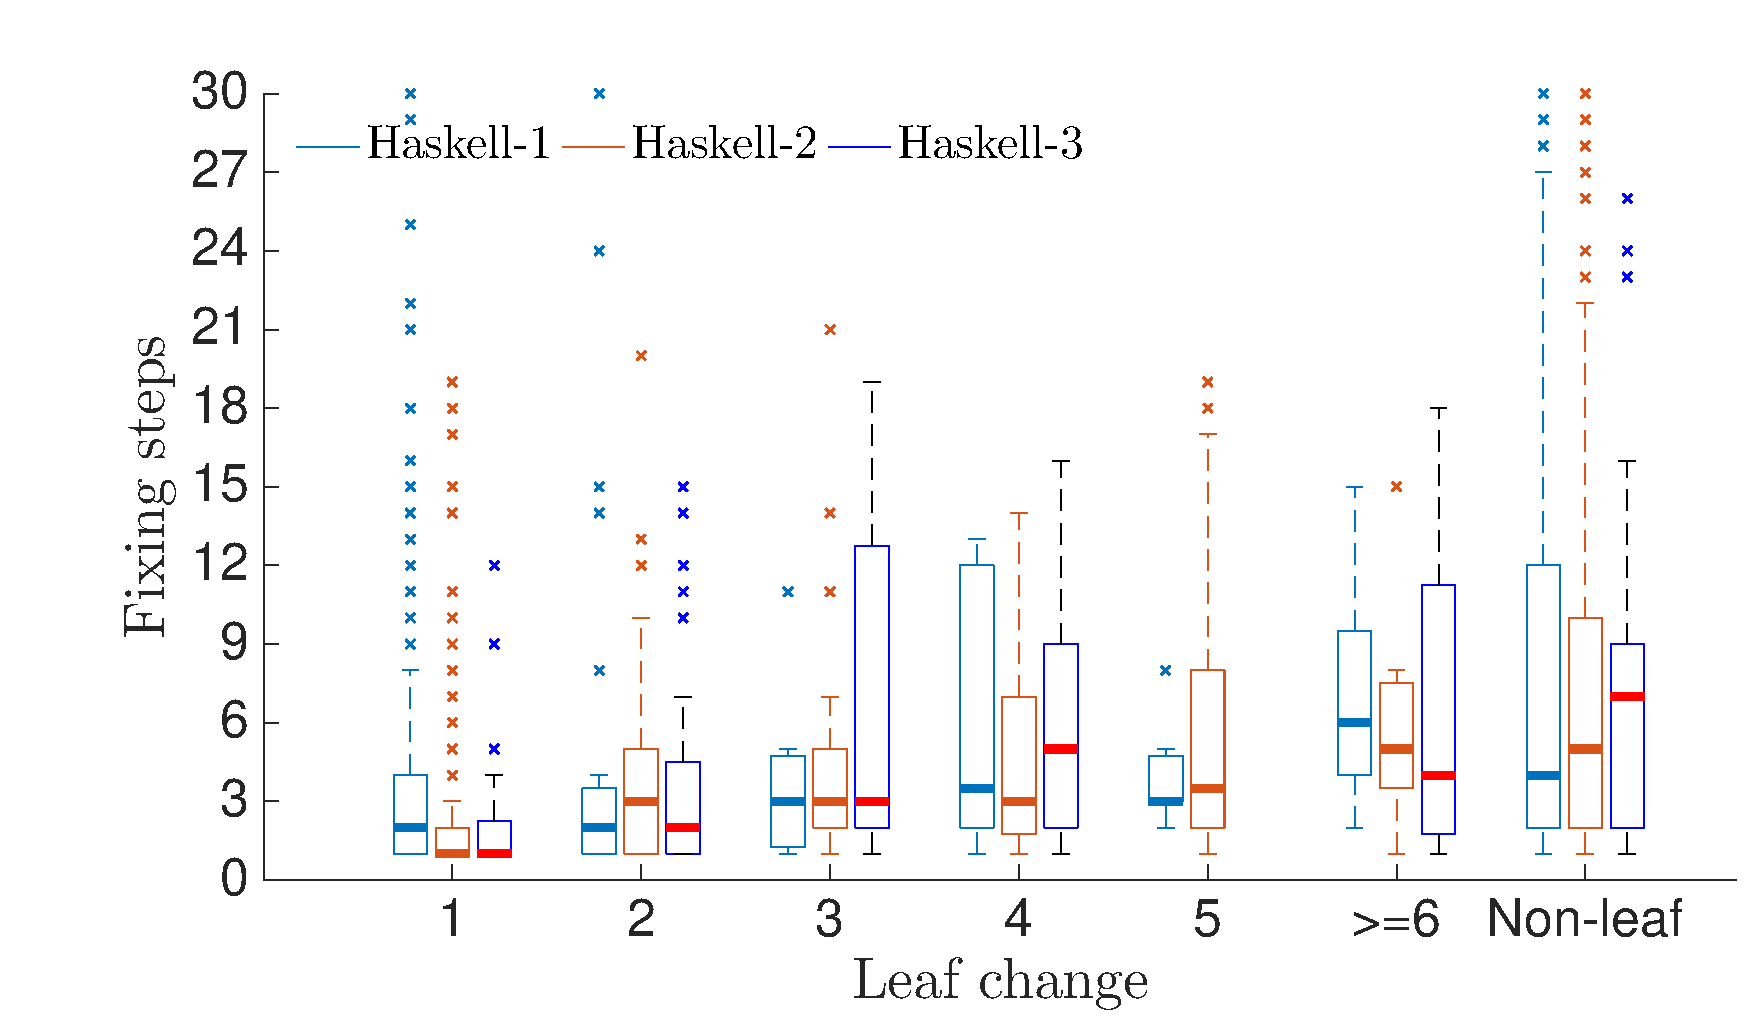
\includegraphics[width=.85\columnwidth]{images/leaf_step.eps}
\caption{The relation between leaf changes and the
number of steps to fix the type error}
\label{fig:lst}
\end{figure}

We conclude that in practice most error
debuggers won't work well since
type errors are
often not caused by single leaves.
Seminal could search for type errors that
are not caused by leaves
%the causes that are not at leaves for type errors,
but it does not achieve a high error locating
accuracy~\cite{Zhang14:tgd,CE14popl}.
Therefore, it would be useful to develop
an error debugger that fixes non-leaf errors
systematically.


\section{Were Type Annotations Reliable?}
\label{sec:annotation}

Since compilers and many error debuggers always trust type annotations,
it is important to study the reliability of type annotations.
%
%
In this section, we define the ratio of wrong type annotations
as the number of type errors containing 
%We first investigate the ratio that students made mistake on type annotations
%as the number of type errors containing 
wrong type annotations 
over the number of all type errors.
%
Based on the final fix record, the ratio of wrong type annotations
is 28\% 
for \benchf, 34.4\% for \benchs, and 
27\% for \benchl. 
%
The result means that, in general, error debuggers can not
precisely locate the real error causes for around 30\% of
type errors if they always trust type annotations. 

The ratio is surprisingly high,
and we investigated why this happens.
%
We found out two main reasons that cause wrong type annotations
to appear frequently.
The first one, called wrong definitions, is that
students wrote wrong type annotation at the beginning.
The other, called out-of-synchronization,
is that students forgot to update type annotations
after they changed the related function definitions.
For example, in \benchs, the ratios for wrong definitions and
out-of-synchronization are 31.3\% and 30.6\%,
respectively.


\begin{figure}
\centering
\begin{tabular}{  c | c | c | c | c | c | c | c | c | c }
\toprule
  Week & 1 & 2 & 3 & 4 & 5 & 6 & 7 & 8 & Average of weeks\\
\midrule
  \benchf & 0.18 & 0.29 & 0.36 & 0.38 & 0.36 & 0.26 & 0.28 & 0.28 & 0.30 (\std=0.07) \\ 
  \benchs &  0.16 & 0.23 & 0.43 & 0.41 & 0.53 & 0.29 & 0.25 & 0.26 & 0.32 (\std=0.12)  \\ 
\bottomrule
\end{tabular}
\caption{Ratio of wrong type annotations}
\label{fig:at}
\end{figure}

We are also interested in knowing if
the ratio of wrong type annotations will be affected
as students were more exposed to
%became more familiar with 
functional programming and the language.
In Figure~\ref{fig:at}, we present the ratio of 
wrong type annotations of each week in
\benchf\ and \benchs. We do not present the
result for \bencht\ because it covers only
three weeks so far.
%
In the first week,
the ratios of wrong type annotations in both program data sets are low
since the programming assignments were simple
and the programs were small~\cite{Hage09:Neon}.
After week 1, students started to make more wrong type annotations
as the assignments became more difficult.
In particular, the highest ratio
in \benchf\ is 0.38 (in week 4) and that in
\benchs\ is 0.53 (in week 5).
%
In later weeks, as students 
were exposed more to Haskell programming,
the ratio of wrong type annotation decreased a little. 
Nevertheless, the average ratio over 8 weeks is about 30\% with relatively small \std\ in both data sets,
which implies that wrong type annotations 
seems to be a constant problem.


\begin{figure}
\centering
%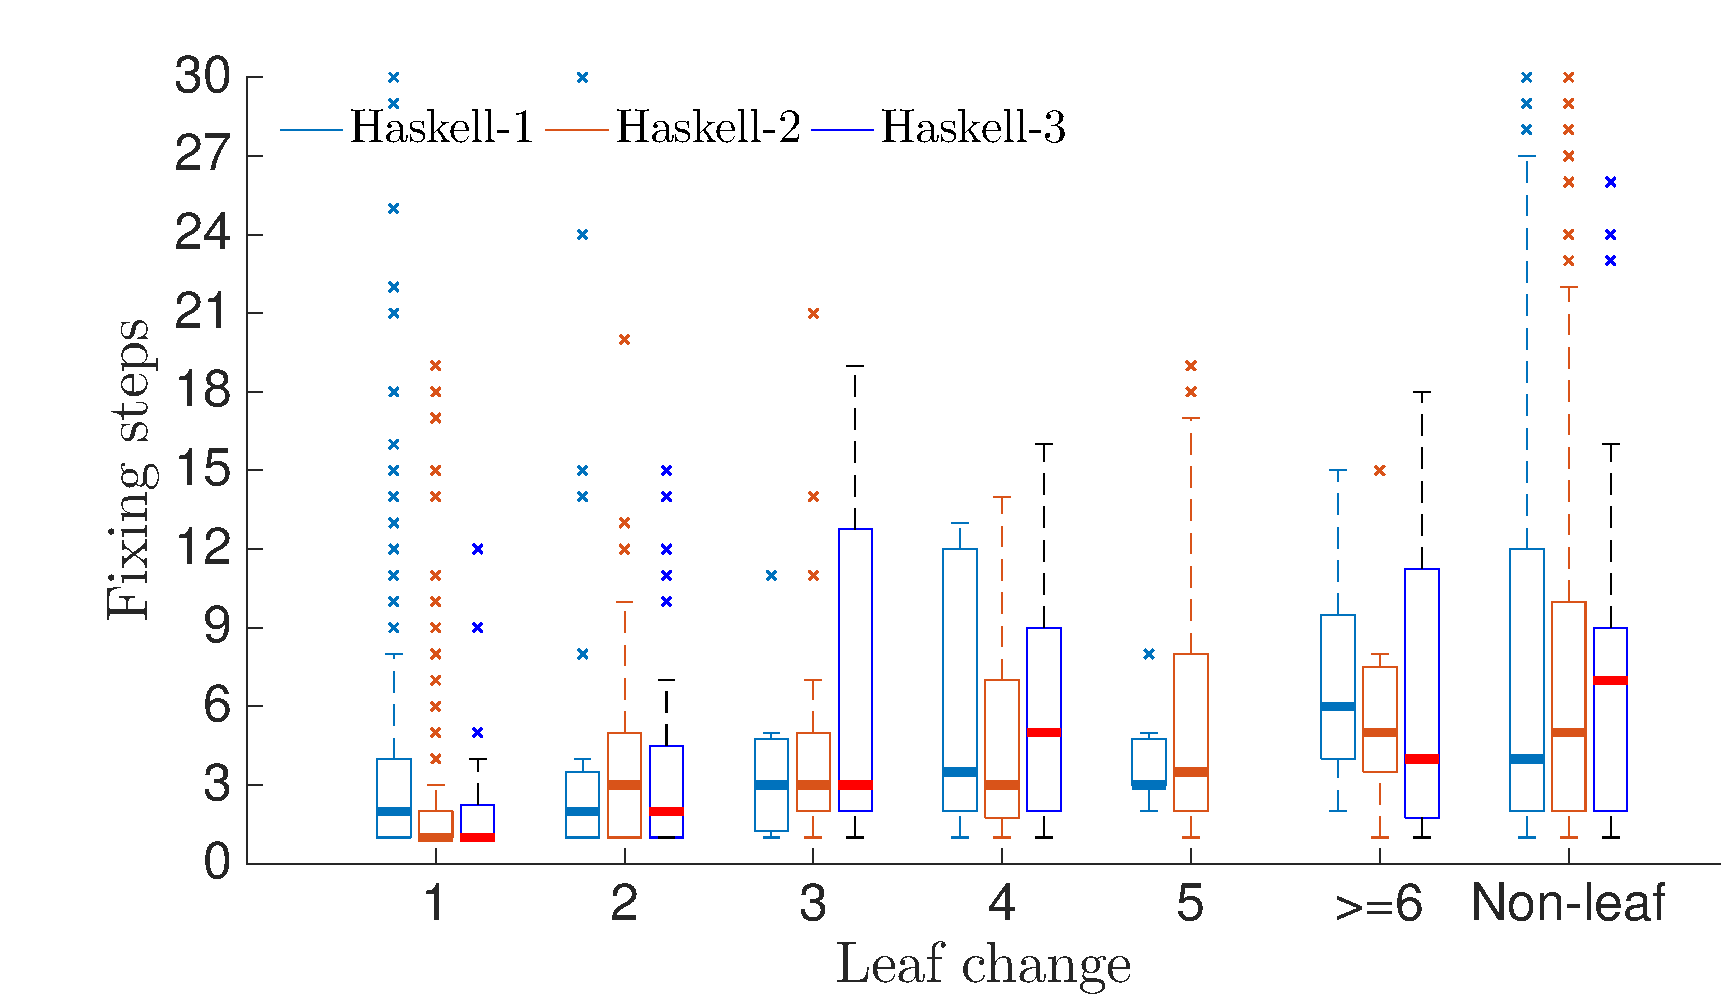
\includegraphics[width=1\columnwidth]{images/leaf_step-eps-converted-to.pdf}
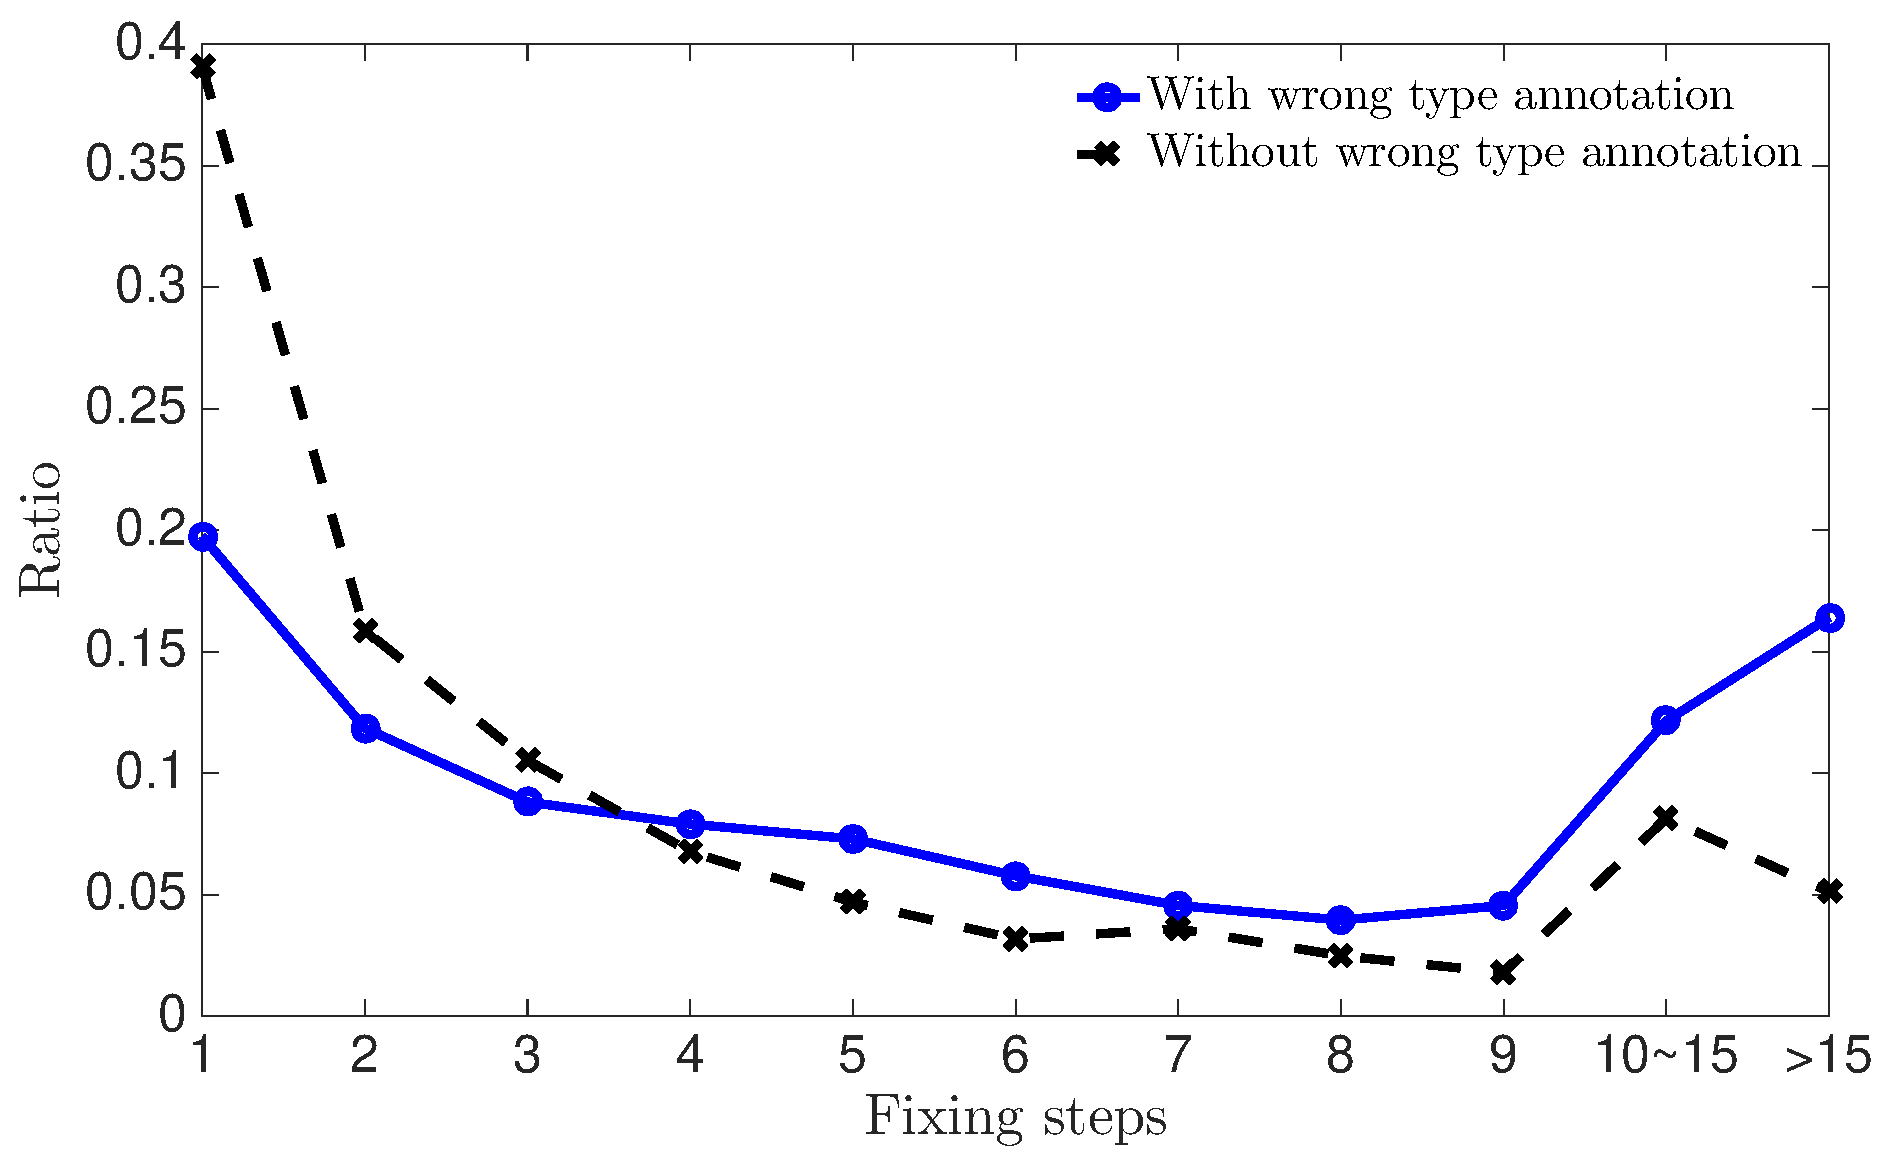
\includegraphics[width=.85\columnwidth]{images/wtn_comp.eps}
\caption{Effect of wrong type annotation on fixing steps}
\label{fig:wtn}
\end{figure}

Next, we study whether the presence of wrong type annotations affects
type error debugging or not.
The average steps for fixing type errors with
wrong type annotations in \benchs\
is 8.1 (\std=8.7), which is greater than 5.1,
the average number of steps for fixing
all type errors according to Section~\ref{sec:overview}.
%
We had the similar results for \benchf\ and \benchl.
Therefore, in general, fixing type errors with wrong type annotations
is more challenging for students than fixing other errors.
%
Moreover, in Figure~\ref{fig:wtn}, we present the distribution of 
numbers of fixing
steps for type errors with and without
wrong type annotations by merging
all the three data sets.
%\benchf\ and \benchs. 
When the number of fixing steps is smaller than 4,
We observe that the ratio for correct type annotations
is higher than that for wrong type annotations. 
%
%\benchf\ and \benchs. 
However, this phenomenon is reversed when the number of 
fixing steps is larger than 4. 
%
For example, for type errors with correct type annotations,
39\% of them can be fixed with single steps
and about 13\% of them need more than 10 steps to fix.
In contrast, those numbers are 20\% and 29\% for the wrong
type annotation case, respectively.
%20\% of the type errors with wrong type annotations are fixed with 1 step,
%and about 29\% of them need more than 10 steps to fix.
%

These results above indicate that it is difficult
for students to fix type errors when
wrong type annotations are involved.
One reason could be that Helium cannot
generate informative messages when type annotations are wrong,
%
Consider, for example, the following student program.
%
\begin{program}
lengte :: [[a]] -> [Int]
lengte x = maximum (map (length.head) x)
\end{program}
%
Helium produces the following error message.
%
\begin{program}
(33,12): Type error in right-hand side
 expression       : maximum (map (length . head) x)
   type           : Int
   does not match : [Int]
\end{program}
%
This error message led the student to inspect
the expression \prog{maximum (map (length . head) x)}
at line 33. Later, the student indeed changed it.
However, the correct fix should change the type annotation
from \prog{[[a]]->[Int]} to \prog{Table->Int} at line 32,
which is far away from the location reported in the error message.


To sum up, type annotations are not reliable,
especially in the beginner programs.
In addition, the error messages related to wrong type annotations
could be ineffective or even misleading,
and debugging wrong type annotations is difficult to students.
Worse, wrong type annotations happen together quite often
with other type errors, making the 
detection of them particularly challenging.

\section{When Are Error Message Effective?}
\label{sec:effectiveness}

Error messages generated by different debuggers
or even the same debugger
contain different kinds of messages, where some messages are more
concrete than others. In general, there are four kinds
of messages with increasingly
concrete information: \typel, \typet, \typer, and \typee.
For example, both \toolS~\cite{Zhang14:tgd,Zhang15:DTE} and  \toolMin~\cite{Pavlinovic14:FMT,Pavlinovic15:PST} generate
the first kind of messages only, which contains
location and the constraint that fails to solve.
All CFT~\cite{CE14popl}, Seminal~\cite{Lerner07:STM}, and
Helium can generate the latter three kinds of messages.
Our goal in this
section is to find out if certain kind of messages are
more effective than other kinds for debugging type errors.
%
We use \benchf\ and \benchs, 
which used Helium as the underlying compiler,
to analyze the message effectiveness, but exclude
\benchl\ since GHC doesn't have all kinds of error messages mentioned above.


The \typet\ kind message reports the inferred type and expected type
for the erroneous subexpression, which are also contained in
\typer\ and \typee\ kinds of messages.
The error message for \prog{lengte}
in Section~\ref{sec:annotation} belongs to this kind. 
The \typer\ kind
message explains the type error in a short sentence, and
%
one such example is the message for \prog{maxLength} in
Section~\ref{sec:subject:metric}. Finally, the \typee\ kind message
%
contains direct information about how to change the program
source code. 
Helium generates such a message for the following student program,
where it suggests to change \prog{(++)} to \prog{(:)}.
%
\begin{program}
toFirst :: [Int] -> [Int]
toFirst (x:xs) = x ++ toFirst (xs)

(3,22): Type error in variable
 expression       : ++
   type           : [a] -> [a  ] -> [a  ]
   expected type  : Int -> [Int] -> [Int]
 probable fix     : use : instead
\end{program}

\noindent
To study the effectiveness of error messages,
we first define the notion of \emph{error situation}, which are three
digits representing:
\begin{enumerate*}[label=(\alph*)]
\item does Helium locate the real error cause correctly,
\item whether following Helium's change suggestion will bring
the current program to the reference program, and
\item the distance between the real error cause and the one reported
by Helium in terms of the number of identifiers.
\end{enumerate*}
%
We have presented them in Section~\ref{sec:subject:metric} but reproduced them
here for the readability purpose.
For example, ``001'' means that Helium failed to locate the real error cause,
and following the message will not bring the program to the reference,
and the location Helium reported is 1 identifier away from the
real error cause.
%
The introduction of error situations is not to evaluate
the quality of Helium's error messages,
but rather to understand how different kinds of messages
affect error debugging in practice.


\begin{figure}
\centering
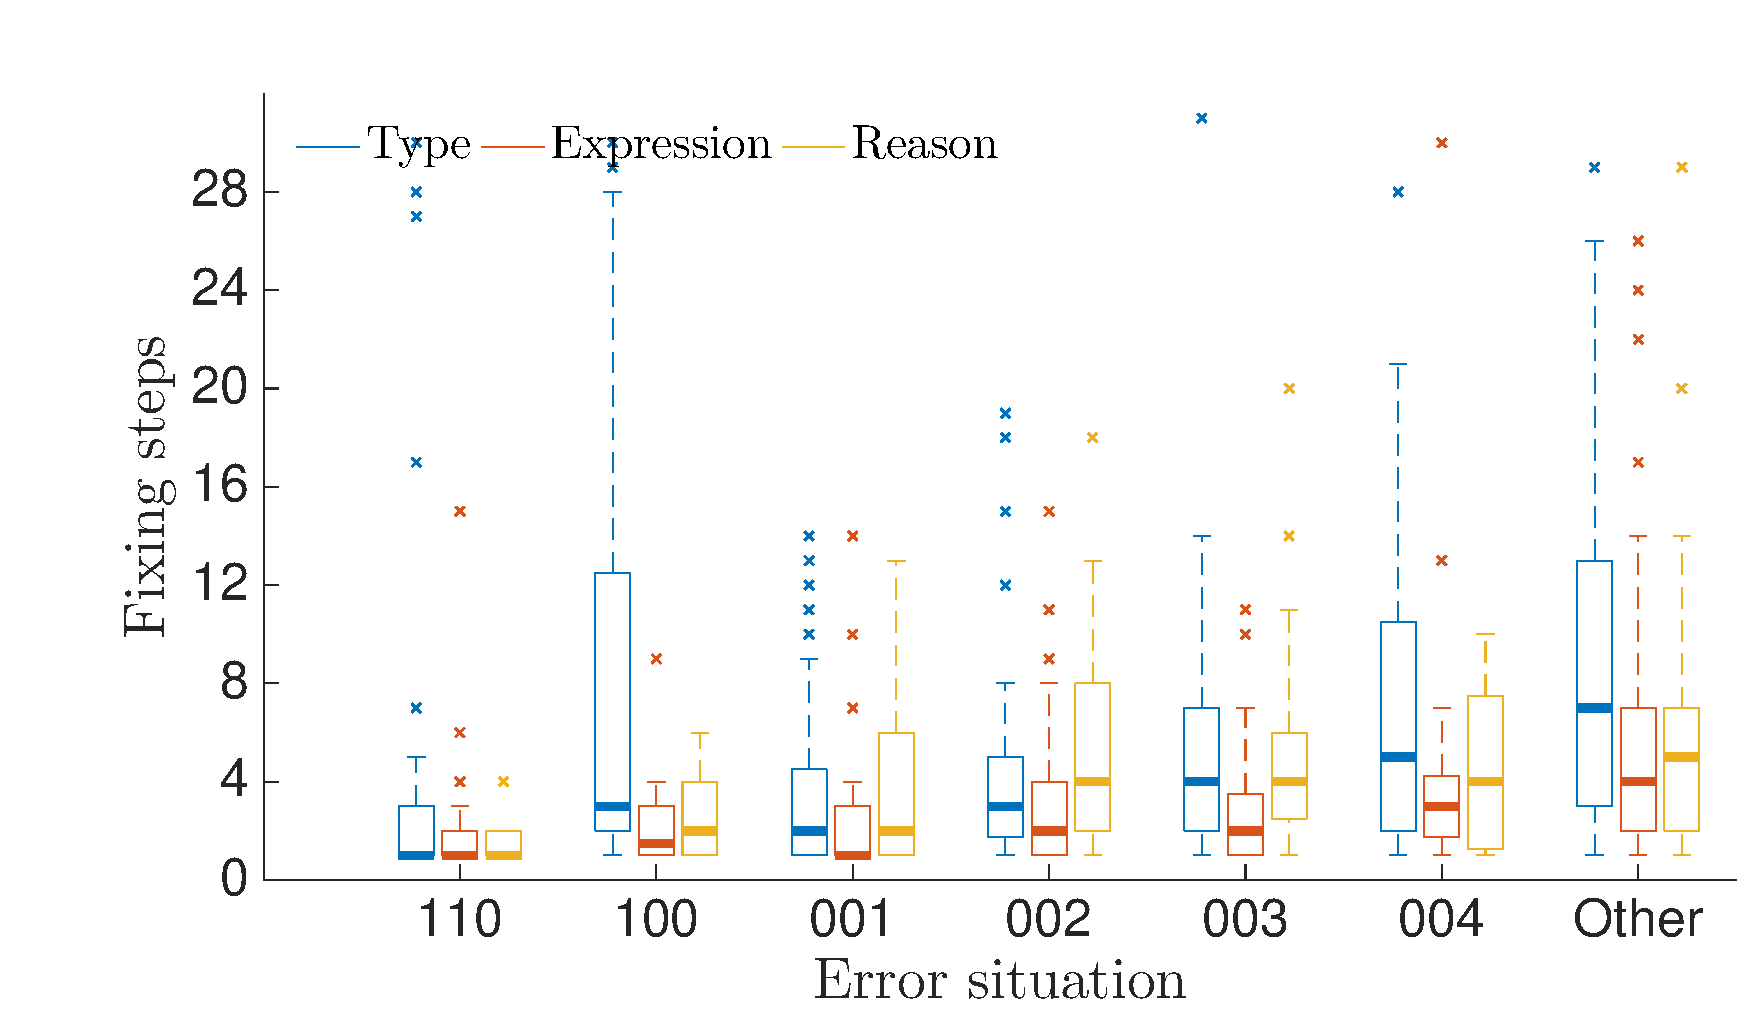
\includegraphics[width=0.85\columnwidth]{images/step_test.eps}
\caption[Error situation against fixing steps]{Error situation against fixing steps. The first digit
of each error situation denotes whether the message locates
the real error cause correctly (``1'') or not (``0''), the
second digit denotes whether following the message will bring
the corresponding program to the reference (``1'') or not (``0''), 
and the third digit measures the distance between the real error
cause and the location reported by Helium in terms of 
the number of identifiers.}
\label{fig:errsitu1}
\end{figure}

We can now classify each error message into one error situation
and further into one of the three kinds:
%For each error situation, we can classify a message into it.
%Furthermore, we classify a message based on one of the three message kinds, namely 
\typet, \typer, or \typee.
%
To measure the impact of error situations and message kind on
error debugging effectiveness, 
we use two metrics: the number of fixing steps and the size differences.
The number of fixing steps is calculated as, from the current programs,
how many steps are needed to reach the reference program.
%
An error situation with large number of fixing steps
indicates a hard debugging case.
%
We compute the size difference by comparing the next version of the current ill-typed program
and the reference.
A large size difference indicates that 
the program in the next step diverges to the reference,
and consequently students don't handle
the current error situation properly.

Figure~\ref{fig:errsitu1} shows the impact of 
different error situations and kinds of 
messages on fixing steps by merging \benchf\ 
and \benchs.
%
In general, we observe that
error situations and kinds of messages affect 
error debugging in the following aspects. First, 
as the reported location becomes further away from 
the real error cause, the number of fixing steps, 
for all message kinds, increases. 
%
The correlation coefficient between fixing steps and 
distances from the reported locations to real error causes
%with respect to the accuracy of error localization 
is 0.53 (\emph{p}-value=$1e^{-15}$). 
%
Second, 
%
the \typet\ kind error messages yields the largest
number of fixing steps for almost all error situations and
%
the \typee\ kind error messages yields the smallest
%number of fixing steps 
for any error situation.
%
%
More specifically, the average number of fixing steps
is 7.7 (\std=10.6) for the kind \typet, 
4.6 (\std=4.5) for the kind \typer, 
and 3.5 (\std=4.2) for the kind \typee.
%
The results show that, regardless of error situations,
type error debugging is less challenging to students when
error messages are more concrete. 

\begin{figure}
\centering
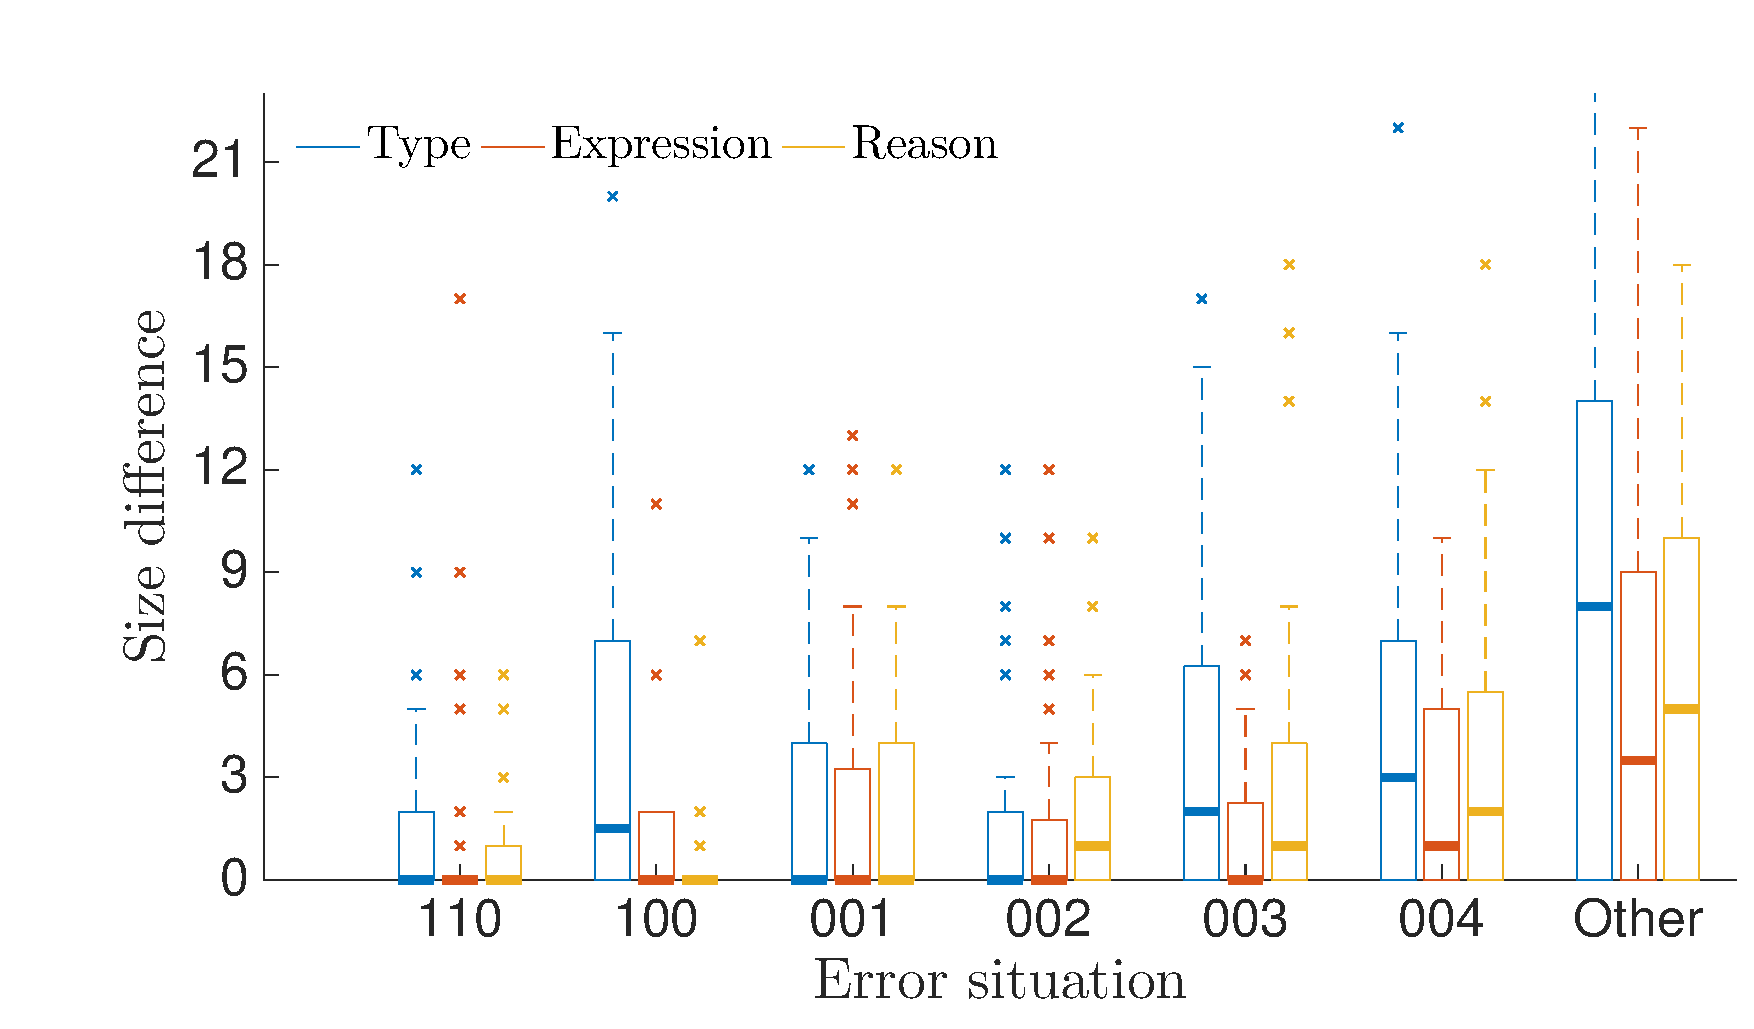
\includegraphics[width=0.85\columnwidth]{images/size_test.eps}
\caption[Error situation against size differences]{Error situation against size differences. The coding
scheme of error situations is the same as that 
in Figure~\ref{fig:errsitu1}.}
\label{fig:errsitu2}
\end{figure}

Figure~\ref{fig:errsitu2} shows the impact from
the perspective of size differences. We make similar 
observations from this figure as what we made from
Figure~\ref{fig:errsitu1}. 
%For example, the error
%situation ``110'' is most effective compared to
%other error situation. 
The size difference
becomes larger as the reported error location becomes
further away from the real error cause, with the
correlation coefficient being 0.48 (\emph{p}-value=$1e^{-15}$).
Moreover, within all error situations, the \typet\ kind
error message yields the largest size difference, with
an average of 5.6 (\std=6.4), while the average size differences
for the kinds \typer\ and \typer\ are 
4.1 (\std=5.5) and 2.7 (\std=4.9), respectively.
%
These numbers imply that more concrete and precise messages
are more useful for students to fix type errors.

\begin{figure}
\centering
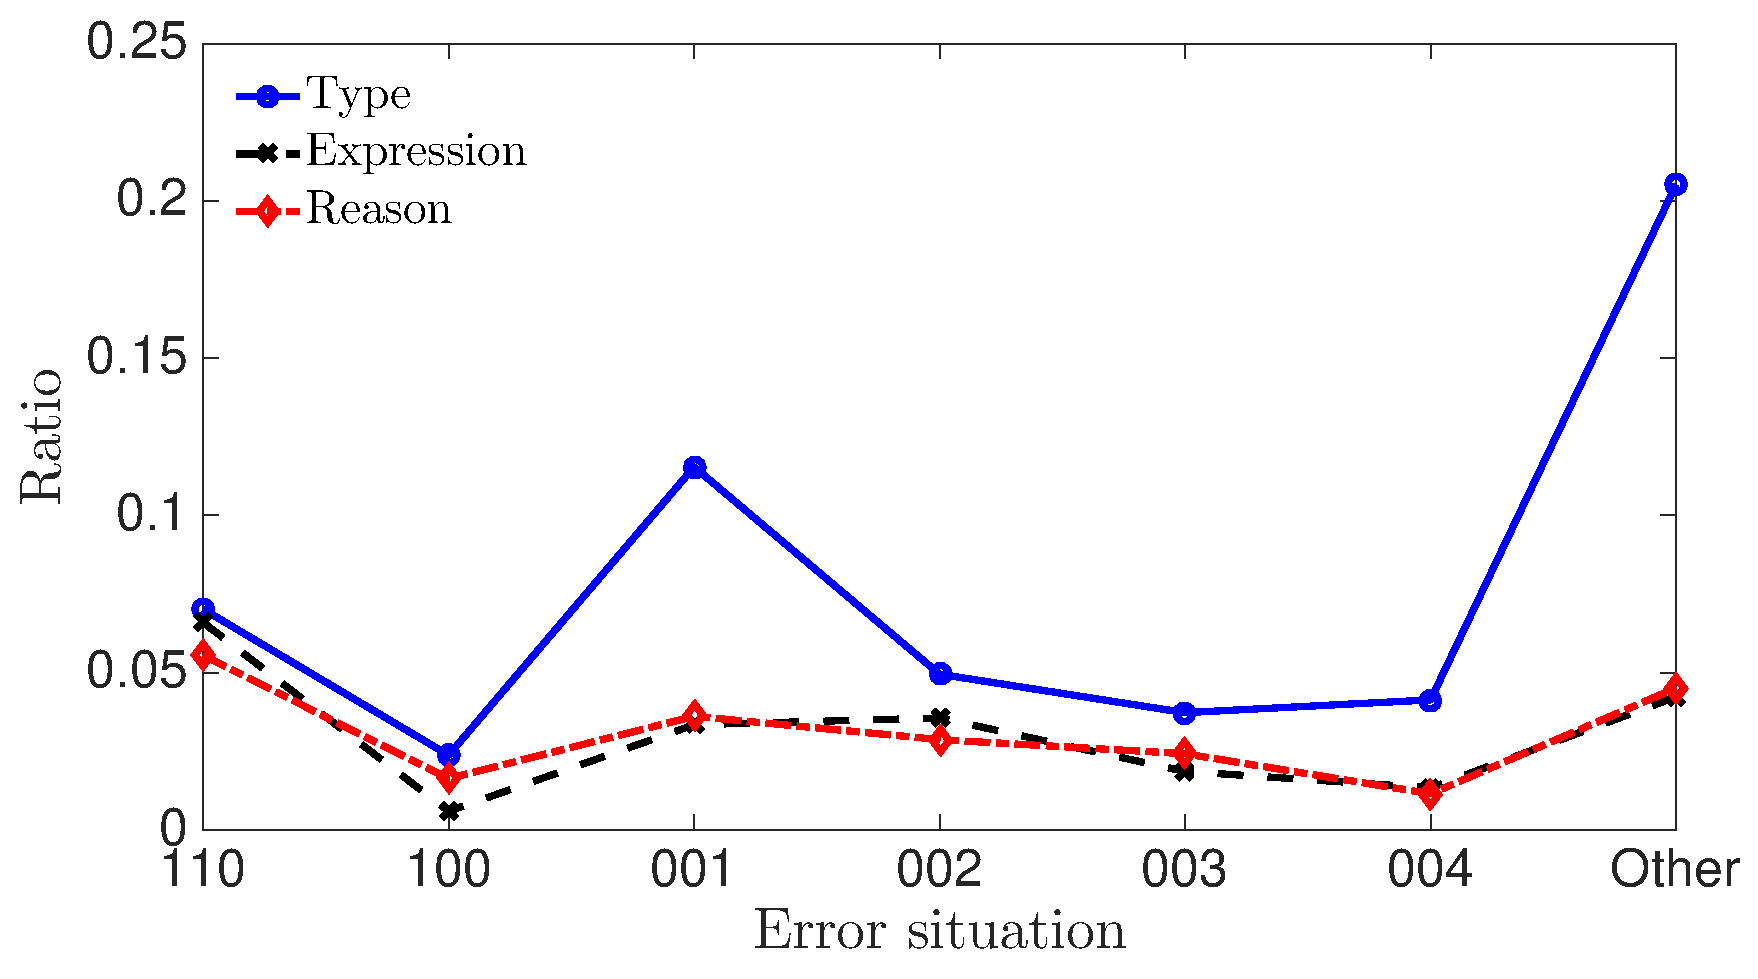
\includegraphics[width=0.85\columnwidth]{images/error_ratio.eps}
\caption{Distribution of error situation}
\label{fig:er}
\end{figure}

Error situations like ``110'' (correct error location and change suggestion)
or ``001'' (1 identifier away from the real error cause) are ideal,
since the number of fixing steps and size differences 
are both relatively small. 
Unfortunately, such situations happen rarely.
Figure~\ref{fig:er} presents the ratios of different situations that
students encountered during debugging type errors,
combining \benchf\ and \benchs\ together.
The ratio for the ideal situation, which we require
the median value 
of fixing steps to be smaller than 4 and that of size differences
to be smaller than 3, is below 10\%, close
to 5\% usually.
Worse,
the \typet\ kind messages appear most often in
all the error situations,
and the ratio is 0.21 in the situation where
the reported location is more than 4 identifiers away
from the real error cause.
This means that the prevalence of less concrete
error messages (the \typet\ kind) in hard debugging
situations (distance larger than 4) exacerbates
the challenges of fixing type errors for students.

We have done the same analysis by considering individual
weeks and have observed similar results. We omit the
details here. The results in this section suggest
that making messages more concrete or 
improving the accuracy of reported error locations
can help debug type errors, especially for novice programmers.

\section{What Language Features Are Difficult?}
\label{sec:difficulty}

In Section~\ref{sec:overview}, we have seen that
the average number of fixing steps in the program data sets 
is around 5.
In this section, we thus
consider type errors that require 
more than 5 steps to fix
as difficult.
%
To study if certain language features are correlated with the
difficulties that students encountered, 
we filtered out all the difficult errors in \benchf, \benchs, and
\benchl, which account for 30.6\% of all errors.
%
For each such error, we manually assign, when appropriate, one
or more difficulty reasons.


We give the meaning of each reason and 
describe how different reasons are assigned 
to a type error in Section~\ref{sec:diffr:reason}, 
where we also justify the selection of each difficulty reason.
Section~\ref{sec:diffr:res} shows some statistical results 
and the impacts of difficulty reasons.
We hope our findings could be exploited
for developing future error debuggers
or could be used to organize course materials
more appropriately.

\begin{figure}
\centering
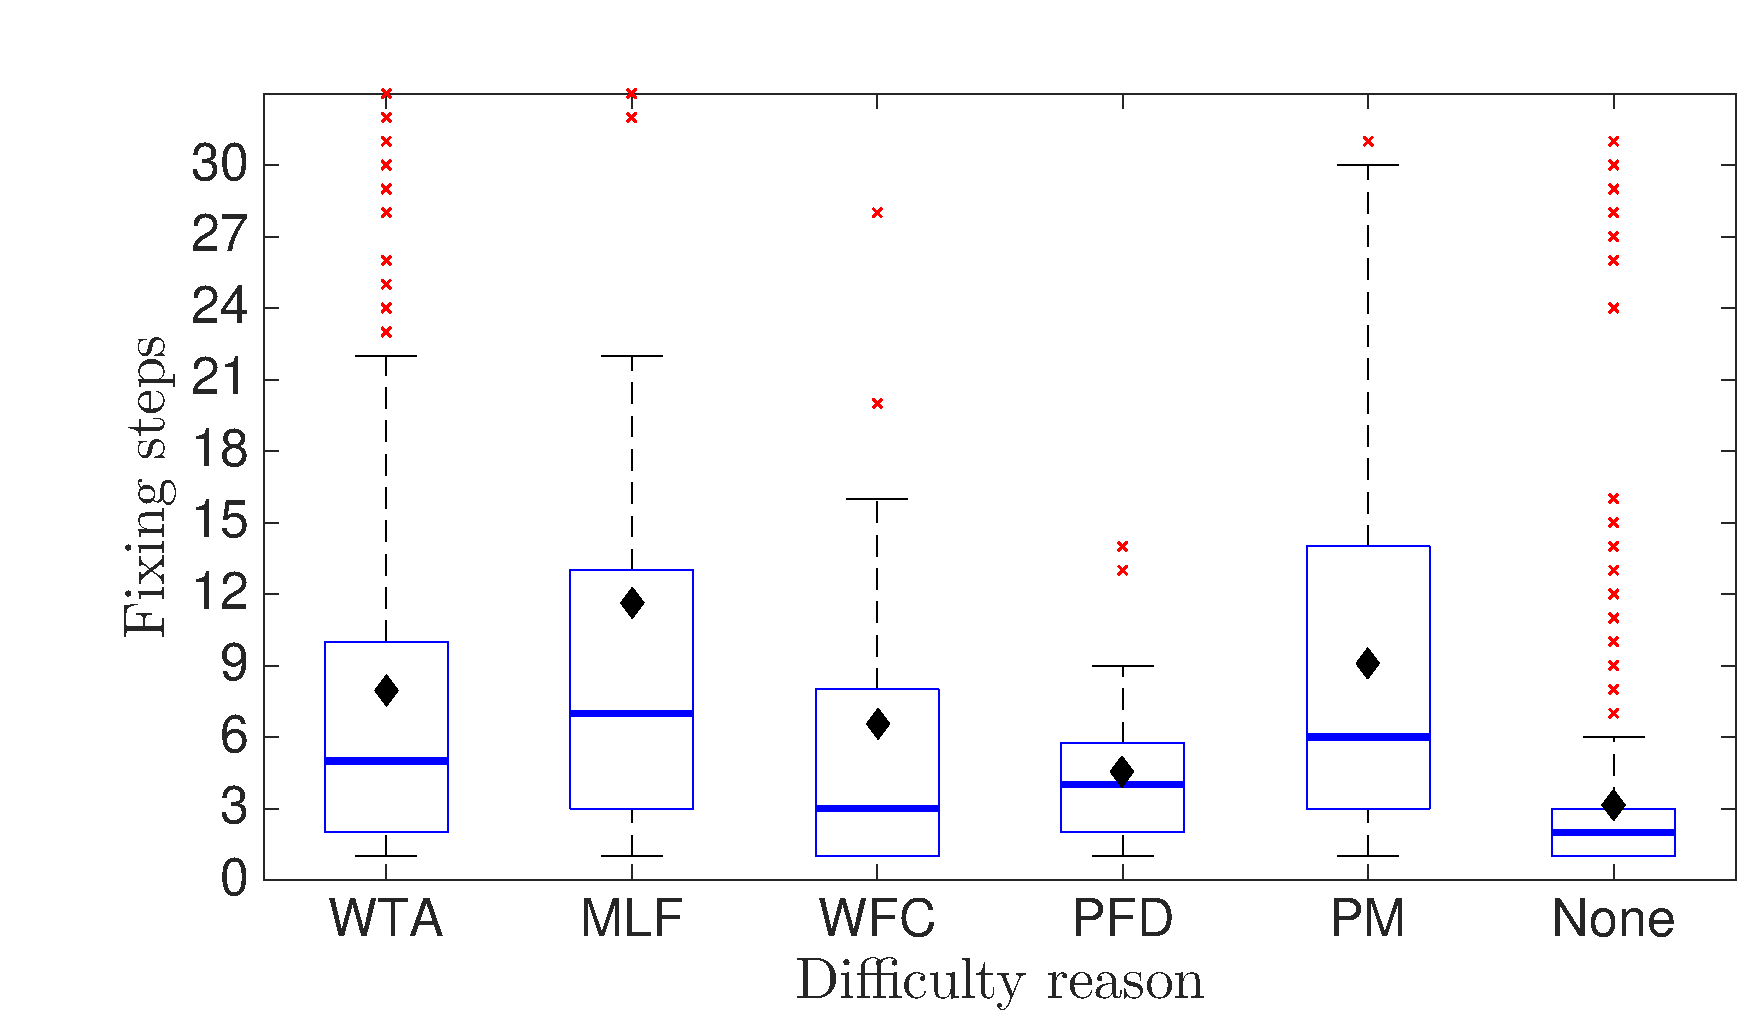
\includegraphics[width=0.85\columnwidth]{images/step_diffr.eps}
\caption[Difficulty reason against fixing steps]{Difficulty reason against fixing steps.
The figure considers all type errors that have the corresponding
difficulty reason, including those that
were fixed within 5 steps.
%
We use a black diamond to represent the average number of steps for each reason.
The average number of fixing steps for all type errors is 5.1 (\std=6.6).
We use the acronyms ``WTA'', ``MLF'', ``WFC'', ``PFD'' and ``PM'' to represent \emph{wrong type annotation}, \emph{multiple library functions}, \emph{wrong function composition}, \emph{point-free function definition}, and \emph{pattern matching}, respectively. ``None'' denotes the errors without assigning any difficulty reason.}
\label{fig:diffr2}
\end{figure}


\subsection{Meanings of difficulty reasons}
\label{sec:diffr:reason}

We found out five main difficulty reasons
that students struggled
when debugging type errors. We identify these
difficulty reasons by comparing the ill-typed
program with the reference program. 
We discuss each difficulty reason below.

\paragraph{Wrong type annotation}
%
We have shown that type annotations are
unreliable and
fixing wrong type annotations usually
needs more effort in Section~\ref{sec:annotation}.
%
%
For example, in the following function
\prog{getTable}, the type error was fixed
by changing the type annotation from
\prog{Table -> String} to
\prog{[String] -> String}, and it
took the student 16 steps to fix. Since only the
type annotation in the ill-typed program is changed in the reference program,
%are the only difference between
%the ill-typed program and the reference program,
we assign ``wrong type annotation'' as the difficult
reason for fixing this type error.
\begin{program}
getTable :: Table -> String
getTable [] = []
getTable (x:xs) = (x ++ "\textbackslash{n}") ++ getTable xs
\it{getTable :: [String] -> String}
\end{program}
%
%
Note that
%, among all type errors including the difficult ones, 
some type errors that are caused
by wrong type annotations can be fixed within 5 steps. 
%Note we can assign this reason to type errors that are fixed
%within 5 steps. 
As a result, it would be interesting to 
know whether this is a real difficulty reason in general.
To address this question, we gathered all the type errors
that were caused by wrong type annotations and investigated
the fixing steps for such errors.
%
Figure~\ref{fig:diffr2} shows that, 
in average, the number of steps to fix these type errors
are 7.9 (\std=8.7), which is larger than that to fix
all type errors.
Therefore, ``wrong type annotations'' is a real difficulty
in fixing type errors. 

\paragraph{Involvement of more than two library functions}
%
When an expression contains more than two library functions,
it usually becomes long and relatively complex.
Since beginners are not very familiar with the types of library functions,
it could be a problem for them to infer whether the whole expression
involving multiple library functions is type correct or not.
%
%
Take the following function \prog{writeLine} as an example, which took
the student 6 steps to fix.
We view that the involvement of multiple library function
as the difficult reason in this example because the use of library functions
\prog{repeat} and \prog{take} complicates the type reasoning,
although the type error is fixed by just changing \progdq{-}
to \progsq{-}.
%
\begin{program}
writeLine :: [Int] -> String
writeLine []     = ""
writeLine (x:xs) = '+' : take x (repeat "-") : writeLine xs
\it{writeLine (x:xs) = '+' : take x (repeat '-') ++ writeLine xs}
\end{program}
%
In Figure~\ref{fig:diffr2}, we present the average number
of steps to fix the type errors caused by this difficulty. 
In average, fixing these type errors took 11.6 (\std=13.1)
steps, which is much greater than
the fixing steps for all type errors. 
Therefore, this
difficulty poses real challenges to error debugging in practice.

\paragraph{Wrong function composition}
%
We observed that type errors are very likely to happen
when \prog{\$}, \prog{(.)}, partial applications,
and parentheses and brackets are used together,
since students do not have good understandings of
associativity and precedence. 
%
In the following example, 
the number of steps to fix the type error in the function \prog{insertionSort} 
is 15.
This error, caused by the mistake of function composition,
is fixed by adding a pair of parentheses around the last
two subexpressions in the body.
%
\begin{program}
insert :: Int -> [Int] -> [Int]
insertionSort :: [Int] -> [Int]
insertionSort lijst = insert (head lijst) insertionSort (tail lijst)
\it{insertionSort lijst = insert (head lijst) (insertionSort (tail lijst))}
\end{program}
%
In average, all type errors assigned with this difficulty reason
took 6.5 (\std=8.7) steps to fix, greater than the 
steps for fixing all type errors. Thus, this is a
real difficulty in fixing type errors. 

\paragraph{Point-free function definition}
%
Point-free functions
help to write compact and clear code. It is
also recommended writing function definitions in
this style when possible.
However, as this style is quite different
from imperative languages that many students are familiar
with, they may take time to get used to it.
We found out that in most cases students changed back
to pointful function definitions
when type errors are related to point-free function definitions.
%In addition, point-free style makes error
%debugging become harder for higher-order functions.
The type error in the function \prog{afterFirst} below
is fixed by adding the parameter to the function definition,
and it took the student 6 steps to fix. Since only the 
function parameter style is changed in the reference program,
we assign ``point-free definition'' as the difficulty reason in this example.
%
\begin{program}
afterFirst :: [Int] -> [Int]
afterFirst = tail \$ dropWhile (/=0)
\it{afterFirst xs = tail \$ dropWhile (/=0) xs}
\end{program}
%
The average number of 
steps students took to fix type errors assigned this difficult
reason is 4.8 (\std=3.4), slightly smaller than
the average number of steps for fixing all type errors. 
%even a little smaller than that average value for all type errors.
However, we still view point-free function definition as one 
difficulty reason because students usually fixed such errors
by ``avoiding'' them rather than by ``overcoming'' them. Specifically,
students fixed such errors by adding parameters to the point-free function definition 
and making corresponding changes in the function body.
%used a workaround to fix this kind of errors
%by using pointful function definitions instead.

\paragraph{Pattern matching}
%
Pattern matching is one of the basic features in
functional programming. Errors in patterns usually
lead to inaccurate and non-informative error 
messages. 
We use the following example
from student program data sets
to show why type errors caused by pattern matching
are hard to fix.
%
\begin{program}
serialization :: [[a]] -> [a]
serialization [h:t] = h ++ serialization t
\it{serialization (h:t) = h ++ serialization t}
\end{program}
%
The error message generated by Helium is:
%
\begin{program}
(6,19): Type error in right-hand side
 expression       : h ++ serialization t
   type           : [a  ]
   does not match : [[a]]
 because          : unification would give infinite type
\end{program}
%
This message fails to locate the real error cause and
conveys the type error in compiler jargon, making
error debugging particularly difficult for students. 
As a result, the type 
error in \prog{serialization} took the student 18 steps to fix. 
%
In Figure~\ref{fig:diffr2}, we present the average number
of steps for fixing type errors that are assigned this difficulty. 
In average, such type errors took 
9.1 (\std=7.9) steps to fix, much more than the steps to fix all type errors.
Therefore, ``pattern matching'' is a
real difficulty in fixing type errors. 

In some cases, we assign multiple difficulty reasons
to a single type error. 
For example, for the type error in the following
function \prog{removeFstColumn}, 
we assign three difficulty reasons (``wrong type
annotation'', ``multiple library functions'',
and ``wrong function composition'') since all of them apply
here. This error took the student 13 steps to fix.
%
%
\begin{program}
removeFstColumn :: Table -> String
removeFstColumn t = transpose.tail (transpose t)
\it{removeFstColumn :: Table -> Table}
\it{removeFstColumn t = transpose (tail (transpose t))}
\end{program}
%

In very few cases, the type errors were obvious to fix 
but still took the student more than 5 steps to fix. We did
not assign any difficulty reason for these cases.
%
For example, the type error in the function \prog{seperator} below is such a case,
which took
the student 6 steps to fix. 
Helium exactly suggests
to change \progdq{-} to \progsq{-} to fix the type error,
but the student 
was maybe not careful enough when debugging the error.
%
\begin{program}
seperator :: [Int] -> String
seperator [] = []
seperator (x:xs) = replicate x "-" ++ seperator xs
\it{seperator (x:xs) = replicate x '-' ++ seperator xs}
\end{program}
%
In other cases that a type error was fixed by rewritting the majority
of the program, we did not assign any difficulty reason either.
%
%
For the type errors we did not assign any
difficulty reason, they took, in average, 
3.1 (\std=4.5) steps to fix. This value is much smaller
than the average number of step for fixing all type error,
suggesting that those errors that are not covered by the five difficulty reasons
will not affect our analysis on the difficulties in fixing type error much.


\subsection{Impacts of difficulty reasons}
\label{sec:diffr:res}

Figure~\ref{fig:diffr1} shows
the distribution of these reasons, where
each ratio is computed as the number of
errors that are difficult
for the corresponding reason over the type errors that took more than
5 steps to fix. All the ratios in the figure do not
sum up to 1 because some errors are assigned multiple
difficulty reasons.
%
It would be meaningful to show how the ratios of
difficulty reasons evolve over the time.
However, 
%since we only considered these difficult
%type errors (the number of fixing steps is bigger than 5),
some weeks do not have enough data for us to perform 
a statistical analysis.

\begin{figure}
\centering
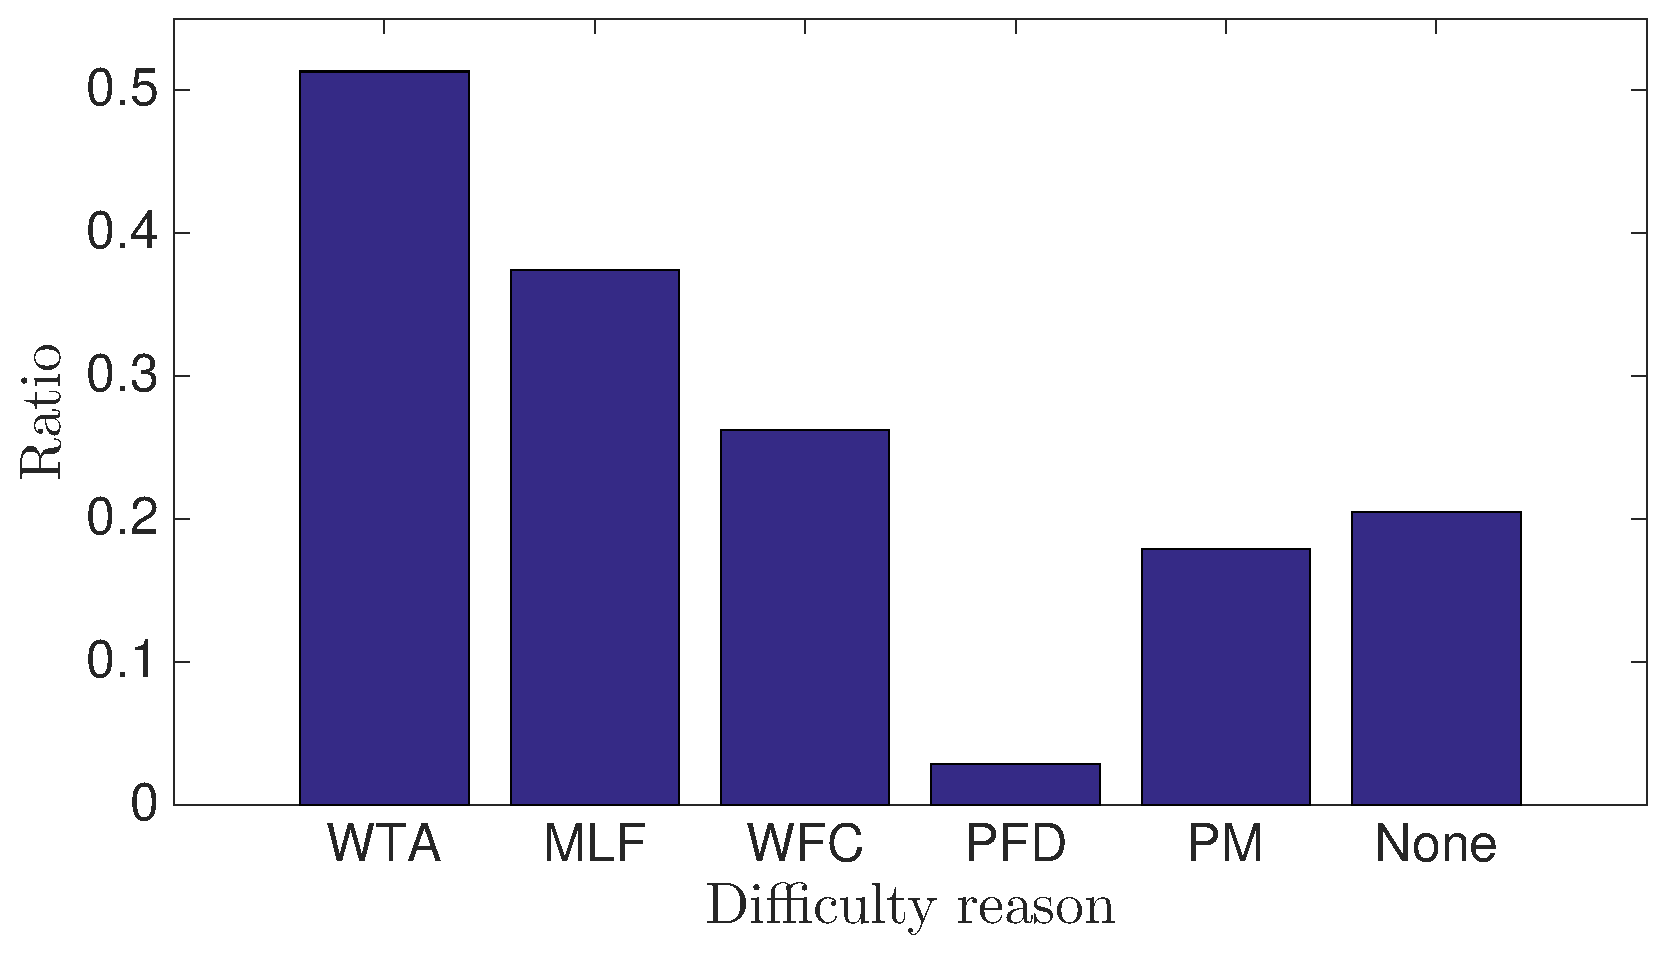
\includegraphics[width=0.85\columnwidth]{images/diffr.eps}
\caption[Distribution of difficulty reasons]{Distribution of difficulty reasons. The figure considers
all type errors that are fixed with more than 5 steps. The labels on 
the x-axis have the same meanings as those in Figure~\ref{fig:diffr2}.
}
\label{fig:diffr1}
\end{figure}


The ratio that students
encountered wrong type annotations as
the difficult reason
is the highest (more than 50\%) among all difficulties.
Unfortunately, we noticed that few 
approaches~\cite{chen2014let} tried
to locate wrong type annotations.
The result indicates that students should check
the correctness of type annotations when they encounter type errors.

About 37\% of the difficult errors are related 
to more than two library functions.
Moreover, we found out that such errors are often assigned
other reasons too, which increases the difficulty in debugging them.
For example, multiple library functions as well as
wrong type annotation and wrong function composition
contribute to the difficulty of fixing
the type error in \prog{removeFstColumn}.
As a result, the average number of fixing steps
for this difficulty reason is the largest in Figure~\ref{fig:diffr2}.
This result suggests that error explanation 
methods~\cite{Chitil01:CET}
could be useful to novice programmers
when debugging this kind of difficult errors.

Wrong function composition accounted for
about 26\% of all difficult type errors.
Note that most error debuggers do not work well
for such errors since they are usually fixed
by adding or removing pairs of parentheses. 
%As shown in Figure~\ref{fig:lst}, such type errors
%take more steps to fix.
From the educational view,
while functional programming languages provide
good flexibility for composing functions,
students might
better defer using them but write nested expressions
with parentheses 
when they first started to learn 
functional programming.

Point-free definitions accounted for 
less than 5\% of difficult type errors.
%
%There are not many type errors (less than 5\%) 
%that are caused by point-free function definition.
This is because students did not use such style
very often. However, as mentioned in 
Section~\ref{sec:diffr:reason}, whenever students
encountered errors with this difficulty, they adopted a workaround to fix
such errors by adding parameters to function
definitions. 
%
Another observation we had while investigating
students programs was that students used point-free
style definitions rarely in their well-typed
parts of programs. 
%
All these findings together imply that students probably did not
comprehend this language feature well.
%We recommend that instructors defer teaching this
%until the students have become proficient with the language.

Pattern matching accounted for about 17\% of all difficult
errors. 
%The ratio of pattern matching errors is only about 17\%,
%which means not many difficult errors belong to this kind.
%However, 
Figure~\ref{fig:diffr2} shows that the average number of steps 
to fix these type errors is the second largest among 
all difficulty reasons.
Mainly this is because that
the generated messages for pattern matching errors
are usually not informative, or even misleading.
To ease the difficulty of debugging such errors,
it is important for students to understand 
correct uses of patterns.

\section{Threats to Validity}
\label{sec:threat}

There are many potential threats to the validity of our study.
First, we have considered only three data sets. Increasing the
number of data sets always increases the validity
of a study. However, due to the particular aspects we are
investigating, many data sets available through git
repositories or Massive Online Open Courses don't
suit our needs. Such data sets contain only final
versions of programs, which are either well-typed or
while ill-typed but we don't have information about
how the type errors should be fixed. Also,
some data set is inaccessible to us due to
permission reasons~\cite{tirronen2015understanding}.
Nevertheless, we have gathered most data sets
available in the research community that suit
our needs. Fortunately, these data sets were written 
%in different languages and 
by different programmers,
used different compilers, and program sizes are quite
diverse, from several lines to several hundred lines.
While two data sets \benchf\ and \benchs\ were collected
at the same university, the programming assignments
were quite different, for example, some assignments
were present in one year while absent in the other year.
For these reasons, we believe that our data sets are quite
representative. Nevertheless, considering
more data sets will give a broader view of error debugging
in practice.


Second, the analysis of fixing process may be affected
by the compiler the students were using. This work
contains two main kinds of analysis, the final fix and the
fixing process. Since the final fix analysis
considered only the ill-typed programs and the final fixed
programs, the result should not be affected by the compiler
being used. The fixing process considered two consecutive
versions by the student, and the second version may
be directed by the error message from the compiler that
was used. However, this issue seems hard to avoid since the
error message has to be generated by some compiler or
error debugger anyways. Moreover, from Figure~\ref{fig:lst},
we observed that the results of using GHC and Helium are
similar. For this reason, we believe that the compilers being
used should pose few threats.


Finally, the majority of the study is performed by me. 
Processing all ill-typed programs
manually is very time consuming.
%, it takes the person
%about 600 hours to finish.
It's hard to allocate
another student to repeat the same work.
We took 
several approaches to minimize the potential biases that
may be introduced.
First, in the beginning, two persons processed
same programs and the results were discussed to
reach agreement. Second, while inspecting
the programs, one person first went through
the whole program sequences to fully understand
users' intention and then analyze each program.
This helped to choose correct reference programs.

\chapter{Representing Type Errors -- \newCompiler\ (I)}
\label{sec:features}

We have reviewed the behaviors of many error debuggers in Chapter~\ref{sec:background},
and we found out that existing approaches are inadequate for handling non-leaf errors (called nonstructural errors in this work), 
which are prevalent in real error debugging scenarios as shown in Chapter~\ref{sec:analysis}.

To better illustrate how the state-of-the-art debuggers perform poorly for fixing nonstructural errors, 
let's consider the following example from the student program dataset~\cite{Hage09:Neon}.
%
\begin{program}
groepeer :: Int -> [Int] -> [[Int]]
groepeer n [] = []
groepeer n x  = take n x ++ groepeer n drop n x
\end{program}
%
This function
tries to group sublists of length \prog{n} of the given list \prog{x}.
The first type error is that, instead of \prog{++}, \prog{:}
should be used. The second
error is that 
a pair of parentheses
is missing around \prog{drop n x}
in the subexpression
\prog{groepeer n drop n x}.

For this ill-typed program, GHC version 8.0.2,
the de facto standard Haskell compiler,
reports the following message.
For simplicity, in the rest of this subsection,
we only show the message 
that is related to the second type error, which is nonstructural.
%
\begin{program}
* Couldn't match expected type `Int -> [Int] -> [Int]'
    with actual type `[[Int]]'
* The function `groepeer' is applied to four arguments,
    but its type `Int -> [Int] -> [[Int]]' has only two
    In the second argument of `(++)', namely `groepeer n drop n x'
    In the expression: take n x ++ groepeer n drop n
\end{program}
%
GHC infers that the recursive call to \prog{groepeer} has too many arguments,
but it fails to make further suggestions about how it could be fixed.

Helium~\cite{Heeren03:HLH}, a Haskell implementation that
focuses on delivering user-friendly error messages for
beginners, reports:
%
\begin{program}
(4,29): Type error in application
 expression       : groepeer n drop n x
 term             : groepeer
   type           : Int -> [Int]               -> [[Int]]
   does not match : Int -> (Int -> [a] -> [a]) -> Int -> [Int] -> [Int]
 because          : too many arguments are given
\end{program}
%
Helium delivers a similar message to GHC, though it's perhaps a bit more readable.
Helium states that too many arguments
are given to \prog{groepeer}. 

SHErrLoc~\cite{Zhang14:tgd,Zhang15:DTE}, another Haskell error
debugger that aims to precisely locate error causes,
blames the type error in the whole subexpression \prog{groepeer n drop n x}


Although the reason given by GHC, Helium and SHErrLoc
provides the right direction for removing the type error, failing to
provide concrete suggestions still poses some challenges to students.
For example, it took students 8 steps to fix the type error in this program.


Seminal \cite{Lerner07:STM} is one of the few error debuggers
that deal with nonstructural errors,
and it usually produces change suggestions to remove a type error.
It does this by searching around the type error's
location
in the program AST and trying to
remove, commute, or change nodes in the AST.
We have translated this program into its equivalent OCaml form,
and the error message generated by Seminal is below.
The presentation of the message is altered by collapsing rows
in order to save space.
%
\begin{program}
Your code has several type errors. The following subexpressions are 
type-correct on their own, but do not fit with the rest of the program:
    @
If you ignore other surrounding code, try replacing: groepeer
with: groepeer; [[...]]
The actual replacement has type
    int -> (int -> 'a list -> 'a list) -> int -> int list -> 'b
within context
    (fun n y -> (match y with
         | [] -> []
         | x -> ((take n x) @; [[...]] ((groepeer; [[...]]) n drop n x))))
\end{program}
%
For this program, Seminal fails to produce a helpful
error message and fix. It suggests to change
\prog{groepeer} to a function
that can take the four arguments
it was erroneously provided, instead of figuring out that a pair
of parentheses needed to be added over the larger subexpression
\prog{drop n x}. 

From the previous error messages, we observe that it's hard to
give good error messages by only considering type conflicts.
We solve 
%Our approach alleviates 
this problem by establishing a statistical
relation between the program information around type errors 
(like the type conflicts and the tree structure)
and how errors are fixed, through machine learning.

In this Chapter, I present the features extracted to represent the program information,
including the type conflicts, the program structure around the error location, and the error messages from the underlying debugger.
Extracting information from the conflicting types is a tricky program, and I investigate the program in Section~\ref{sec:features:unify}.
I discuss the extraction of the latter two kinds of information in Section~\ref{sec:features:feature}.

\section{Unifying Non-Unifiable Types}
\label{sec:features:unify}

When a type error is detected, the underlying compiler usually
provides only the expected type and inferred type of
the identified error cause and the fact that these types fail to
unify. Instead, we need
to extract more meaningful information for machine learning
from them even though they are
non-unifiable.

Even though two types fail to unify,  investigating the
unification process still allows us to capture useful information.
We use the following pair of types to illustrate our discussion below.
%
%\begin{program}
%\begin{align*}
%\text{expected type} : [\tv] \to \Int            & \to \Bool \to \Int \\
%\text{inferred type} : \Int \to (\Int \to \Bool) & \to \tv
%\end{align*}
%\end{program}
\begin{alignat*}{4}
\text{expected type}\ (\mtexp) &: [\tv] && \to \Int            && \to \Bool \to \Int \tag{1} \label{eq:expected}\\
\text{inferred type}\ (\mtinf) &: \Int  && \to (\Int \to \Bool) && \to \tv \tag{2} \label{eq:inferred}
\end{alignat*}
%
The unification of these two types leads to two subproblems:
\mui{[\tv]}{\Int} and \mui{\Int \to \Bool \to \Int}{\Int \to \Bool \to \tv}. We use
the notation \mui{\mt_1}{\mt_2} to denote the unification problem between $\mt_1$
and $\mt_2$.
%
When solving the first
subproblem, the unification fails since we can't unify a list type against
\Int. However, we observe that if we add $[]$ over \Int\ (more formally, applying the
list type constructor to \Int), then these types can be unified. One design
decision we are facing is, should we record \map{\tv}{\Int} in the substitution
returned from solving the first subproblem?
%
There are reasons for choosing either to record or not to record. We decide to record because
the error in the first unification problem is already fixed by adding $[]$
and ignoring \map{\tv}{\Int} will not place correct constraint on later
unification problems.

Solving the second unification subproblem by first substituting \tv\ with \Int, we
further have to solve the following subproblems, which we name as \eqref{eq:unifsub3}
and \eqref{eq:unifsub4}.
%
\begin{align}
\Int & =^?  \Int \to \Bool \tag{3}\label{eq:unifsub3}\\
\Bool \to \Int & =^? \Int \tag{4} \label{eq:unifsub4}
\end{align}
%
Both these subproblems fail to solve because we can't
unify a function type with a non-function type. However,
there is an important difference between them. Namely,
the types constituting the problem~\eqref{eq:unifsub3} are the
argument types of the original types and those constituting
the problem~\eqref{eq:unifsub4} are the return types of the original
types. This distinction is important because the former usually
indicates that a function has been applied to
wrong arguments and the latter indicates
that a function is given not enough or too many arguments.
%We need to distinguish between them. Similarly, we distinguish
%between when $[]$ difference happened.

Overall, we compute four components from two conflicting types:
\begin{enumerate*}[label=(\arabic*)]
\item \TopLevelDiff, which represents the top-level
function difference (-1 in our example),

\item \TopBracketDiff, which represents the top-level bracket
difference (0 in our example),

\item \FuncDiff, a list of location and function difference pairs in
argument types ([(2,1)] in our example), and

\item \BracketDiff, a list of location and bracket difference pairs
in argument types ([] in our case).
%
\end{enumerate*}

\subsection{Computing Type Differences}
\label{sec:unify:alg}

\begin{figure}
\begin{minipage}{1\columnwidth}
\begin{qprogram}
\ofType{\ualg}{\mt \times \mt \times \level \times \idx \to \subtt \times \sieves} \\[3pt]
%
\nameva\ $\ualg(\tv,\mt,\level,\idx)\ |\ \tv == \mt = (\emptyset,\emptyset) $ \\%
\phantom{\nameva\ $\ualg(\tv,\mt,\level,\idx) $} $
                                 |\ \tv \in \FV{\mt} = \dalg(\tv,\mt,\level,\idx,0) $ \\
\phantom{\nameva\ $\ualg(\tv,\mt,\level,\idx) $}
                                 |\ otherwise $ = (\set{\map{\tv}{\mt}},\emptyset)$ \\[3pt]
%
\namevb\ $\ualg(\mt,\tv,\level,\idx) =
    \textbf{let}\ (\subtt,\td) = \ualg(\tv,\mt,\level,\idx)\
    \textbf{in}\ (\subtt,-\td) $ \\[3pt]
%
\namevc\ $\ualg(\mt_1 \to \mt_2, \mt_3 \to \mt_4,\level,\idx)
            = \textbf{let}\ (\subtt_1,\td_1) = \ualg(\mt_1,\mt_3,\level + 1,\idx) $\\
\phantom{\namevc\ $\ualg(\level,\idx,\mt_1 \to \mt_2, \mt_3 \to \mt_4)lll\textbf{let}$}
$    (\subtt_2,\td_2) = \ualg(\subtt_1(\mt_2),\subtt_1(\mt_4),\level,\nextIdx{\level}{\idx}) $\\
\phantom{\namevc\ $\ualg(\level,\idx,\mt_1 \to \mt_2, \mt_3 \to \mt_4)lxl$}
$    \textbf{in}\ (\com{\subtt_2}{\subtt_1}, \union{\td_1}{\td_2}) $ \\[3pt]
%
\namevd\ $\ualg([\mt_l],[\mt_r],\level,\idx) = \ualg(\mt_l,\mt_r,\level,\idx)$ \\[3pt]
%
\nameve\ $\ualg(\mt_l,\mt_r,\level,\idx)\ |\ \mt_1 == \mt_r \phantom{l} = (\emptyset,\emptyset)$ \\
\phantom {\nameve $\ualg(\level,\idx,\mt_l,\mt_r)\ $}
    $|\ \text{otherwise} =\dalg(\mt_l,\mt_r,\level,\idx,0)$ \\[6pt]
%
\ofType{\dalg}{\mt \times \mt \times \level\times \idx \times \depth \to \subtt \times \sieves} \\[3pt]
%\namevf\ $\dalg(\mt_l,\mt_r,\level,\idx,\depth) $\\
%\phantom{xxxx} $ |\ \length(\mt_l) \neq \length(\mt_r) = (\emptyset,(\set{(\level,\idx,\length(\mt_l) - \length(\mt_r))},\emptyset)) $ \\[3pt]
\namevf\ $\dalg(\mt_l,\mt_r,\level,\idx,\depth)$ \\
\phantom{abcd} $ |\ \length(\mt_l) \neq \length(\mt_r) = (\emptyset,(\set{(\level,\idx,\length(\mt_l) - \length(\mt_r))},\emptyset)) $ \\[3pt]
%
\namevg\ $\dalg([\mt_b],\mt,\level,\idx,\depth) =
        \textbf{let}\ (\subtt,\td) = \dalg(\mt,[\mt_b],\level,\idx,\depth)\
        \textbf{in}\ (\subtt,-\td) $ \\[3pt]
%
\namevh\ $\dalg(\mt,[\mt_b],\level,\idx,\depth) = \dalg(\mt,\mt_b,\level,\idx,\depth+1) $ \\[3pt]
\namevi\ $\dalg(\mt,\tv,\level,\idx,\depth) = (\set{\map{\tv}{\mt}},(\emptyset,\set{(\level,\idx,\depth)})) $ \\[3pt]
%
%
\namevj\ $\dalg(\mt_l,\mt_r,\level,\idx,\depth)\ |\ \mt_l == \mt_r\ \  =
(\emptyset,(\emptyset,\set{(\level,\idx,\depth)})) $ \\
\phantom{\namevj\ $\dalg(\level,\idx,\depth,\mt_l,\mt_r)$}
    $|\ \text{otherwise} = (\emptyset,\emptyset) $
%
\end{qprogram}
\end{minipage}
\caption{A type difference algorithm}
\label{fig:ualg}
%\vspace{-1em}
\end{figure}

We develop an algorithm for computing type differences in Figure~\ref{fig:ualg}.
This algorithm doesn't directly compute all the four components
discussed earlier. Instead, we will show this computation towards the end
of this subsection.

The algorithm can be conceptually understood as two parts: the part
that handles normal unification (\ualg) and the part
that computes type difference once unification fails (\dalg).
%
In the
figure, we use the auxiliary function \FV{\mt} to compute the set of
free type variables in \mt\ and use the function $\length(\mt)$ to compute the
number of spines of \mt.
The type \td\ is a pair of two sets, for storing the results
of arrow differences and bracket differences, respectively. The members of the
set has the form $(\level,\idx,v)$, where \level\ and
\idx\ denote the level and the index at where the value $v$ is computed.
We will discuss
more about \level\ and \idx\ in the next paragraph.
%
To simplify the presentation,
we write $\emptyset$ for \td\ to denote that both sets of \td\ are empty.
We use the set union operation to union two \td{s} by taking the union of their respective
components. We also write $-\td$ to negate the third component of each
set member in \td.

The function \ualg\ takes four arguments, the types that are being
unified ($\mt_l$ and $\mt_r$) and the level \level\ and index \idx\
that indicate the nesting level and the index
of $\mt_1$ and $\mt_2$ in the original types, respectively.
The variable \level\ helps us to distinguish whether the result
computed is for top-level difference (if \level\ is 1) or for
arguments (if \level\ is 2). It's rare for \level\ to reach more
than 2 due to how underlying compilers report type errors.
Given an ill-typed expression \prog{f g x}, \level\ may reach
3 only if the type error is reported at \prog{f} and the argument
\prog{g} itself is a higher-order function. However, usually in
such cases debuggers report type error at \prog{g} since this is
a smaller expression that is ill-typed. When \level\ is 2, \idx\
specifies argument at which the type difference is computed. This
information is important because it tells where type mismatch
happens.
For example, if we are now solving
the problem~\eqref{eq:unifsub3} arising from the problem \mui{\mtexp}{\mtinf},
then the \level\ and \idx\ are 2 and 2,
respectively. Similar, for the problem~\eqref{eq:unifsub4},
they are 1 and 3, respectively.
%
We use the function $\nextIdx{\level}{\idx}$ to compute the index, which
returns \idx\ if $\level > 1$ and $\idx+1$ otherwise. We
do this to ensure that for $\level \leq 2$ the pair $(\level,\idx)$
uniquely determines the part of the type.
%
When \ualg\ is first called, both \level\ and \idx\ are initialized to 1.
%
%

%
In addition to these four arguments, \dalg\ takes another argument \depth,
indicating the current depth of the computed bracket difference. Both
\ualg\ and \dalg\ return two values, a substitution mapping type variables
to types and a \td.

We now briefly go through different cases of \ualg\ and \dalg. The structure of
\ualg\ is similar to traditional unification algorithms, except that it doesn't
terminate on unification failure but calls \dalg\ for recording type
differences. Case \nameva\ unifies the type variable \tv\ against the
type \mt. If \tv\ is the same as \mt, then we return $\emptyset$ for both
the substitution and the \td. If the occurs check succeeds, then \tv\ and \mt\
fail to unify, and we use \dalg\ to record the difference. Otherwise, the
unification succeeds and maps \tv\ to \mt. Case \namevb\ is a dual case of
case \nameva. It delegates the real unification to case \nameva\ and takes
the negation of the \td\ returned by \nameva.

Case \namevc\ unifies two function types. We unify their corresponding
argument types and return types, respectively. We also pass in appropriate
level and index values when solving subproblems. The composition of two
substitutions has a conventional definition. When unifying two list types,
we unify the underlying types wrapped in lists. This is handled by case \namevd. Finally,
case \nameve\ takes care of other situations. In particular, if two types are different,
we record their differences using \dalg.

We now turn our attention to \dalg. First, in case \namevf, if two types have
different numbers of spines, then we record function differences.
%
The remaining cases of \dalg\ handle bracket differences. It
always assumes that its second argument has more brackets than its first
argument. As a result, in case \namevg, if the first argument has more
brackets, we call \dalg\ with the types swapped and then take the negation of
the computed \td. In case \namevh, if the second type is a list type, then
the bracket difference is increased by one and \dalg\ is recursively
called. Note that in case \namevh, the first argument couldn't be a list type.
Otherwise, the case would have been captured by case \namevd\ of \ualg.
Next, the case \namevi\ handles the situation that the second argument
is a type variable \tv. We solve this case by mapping \tv\ to the first
argument and recording the bracket differences at the same time. Finally,
if two types are the same, we record bracket differences. Otherwise, if
$\mt_l$ and $\mt_r$ are different, we don't record any bracket difference.
The reason is that the type error couldn't be fixed by adding or removing
brackets.

Given a $\td=(F,B)$, the \TopLevelDiff\ is $v$ if $(1,\idx,v) \in F$
for some \idx\ and 0 otherwise. The \FuncDiff\ collects all the pairs
$(\idx,v)$ such that $(2,\idx,v) \in F$. Similarly, we can
compute \TopBracketDiff\ and \BracketDiff\ from $B$.

Usually error debuggers include the difference between two
conflicting types as a heuristic to rank all potential error
causes~\cite{Chen14:CFT,Hage07:HTE}. The computations in these
approaches are quite simple, for example, just computing the
difference between the arities of conflicting types. Our
algorithms \ualg\ and \dalg\ could be employed for that purpose
and give more precise results.

\subsection{Properties}
\label{sec:unify:prop}

In this subsection, we investigate the properties of \ualg\ and \dalg. First, both of
them are terminating, as captured in the following theorem.

\begin{theorem}
For any two types $\mt_l$ and $\mt_r$, $\ualg(\mt_l,\mt_r,1,1)$ terminates.
\end{theorem}
%
\begin{proof}
We give a proof sketch based on four observations.
First, in all cases of \ualg,
except case \namevb, case \nameva\ second guard, and case \nameve\
second guard, the sizes of types to the recursive calls of \ualg\
decrease. Moreover, the case \namevb\ can only be called once and
other two cases are handled by the termination of \dalg.
Second, in all cases of \dalg, except case \namevg, the sizes of
types to all recursive calls decrease. Moreover, case \namevg\ can
be called only once. Third, \dalg\ doesn't call \ualg, so \ualg\ and \dalg\
are not mutually recursive. Finally, all auxiliary functions are terminating.
As a result, \ualg\ is terminating.
\end{proof}

We want \td\ to capture only  differences
between types, though we don't
record all information about the
differences of types. We only
try to capture information useful
to type error debugging.
Consequently, if the types are unifiable, then \ualg\ returns an empty \td, as captured in the
following theorem.
%
\begin{theorem}
\label{the:sound}
If $\mt_1$ and $\mt_2$ are unifiable,
then $\ualg(\mt_1,\mt_2,1,1)=(\subtt,\emptyset)$ for some \subtt.
\end{theorem}

\begin{proof}
If two types are unifiable, then the conditions of
case \nameva\ second guard and
\nameve\ second guard can't be satisfied, and \dalg\ will not
be called. As a result, the \td\ will be empty.
\end{proof}

Unfortunately, the opposite of Theorem~\ref{the:sound} doesn't hold.
That is, if the \ualg\ computes empty \td, it doesn't mean that
the two types are unifiable. Also, \td\ doesn't capture unification
failure caused by other type mismatches. However, \ualg\ and
\dalg\ do capture authentic arrow differences and bracket differences.
We express this result in the following theorem.
%
\begin{theorem}
Given \mtf\ and \mts, let $\mt_{1p} = \restrict{\mtf}{(\level,\idx)}$,
$\mt_{2p} = \restrict{\mts}{(\level,\idx)}$, and $(\subtt,(F,B)) = \ualg(\mtf,\mts,1,1)$, then for any $(\level,\idx)$ with $\level < 3$  then $(\level,\idx,f) \in F$ if and only if $\length(\subtt(\mt_{1p})) \neq \length(\subtt(\mt_{2p}))$. Similarly, $(\level,\idx,b) \in B$ if  $\subtt(\mt_{1p})$ and $\subtt(\mt_{2p})$ differ by $b$ brackets.
%
\end{theorem}
%
In the theorem, we write \restrict{\mt}{(\level,\idx)} to get the
part of the type \mt\ at level \level\ and index \idx. The pair $(\level,\idx)$
determines the location when $\level < 3$. For example, $(2,2)$ refers to the type
\Bool\ in type~\eqref{eq:inferred} and $(2,2)$ refers to the first \Int\ in
the type~\eqref{eq:expected}.
%
This theorem can be proved by an induction over each case of \ualg\ and \dalg. The reason there is no "only if"
clause for bracket difference is that
recording function differences takes
priority in our algorithm. As an
example, for $\Int\ \to\ \Bool =^?
[\Int\ \to\ \Bool]$, the arity
difference makes the function
difference rules take priority, even
though the types differ by 1 bracket.

\section{The Feature Vector}
\label{sec:features:feature}

\begin{figure}
\centering
\begin{tabular}{c | l l}
\toprule
ID &  Summary   &  Feature Values  \\
\midrule
1 & Kind of the error message from Helium. & Nominal (1 $\sim$ 13) \\
2 & Kind of change suggestion in the error message. & Nominal (1 $\sim$ 3) \\
3 & Type differences between the conflicting types & \IntVal\ ($\ge$ 0) \\
%3.1 & Top-level function difference of the conflicting types. & \IntVal\ ($\ge$ 0) \\
%3.2 & Top-level bracket difference of the conflicting types. & \IntVal\ ($\ge$ 0) \\
%3.3 & Function difference of the conflicting types. & \IntVal\ ($\ge$ 0) \\
%3.4 & Bracket difference of the conflicting types. & \IntVal\ ($\ge$ 0) \\
4 & Location of type inconsistency in AST. & Nominal (1 $\sim$ 3) \\
5 & Kind of the offending location. & Nominal (1 $\sim$ 6) \\
6 & Associativity of the operator in Feature 5. & Nominal (-1, 1, 2) \\
7 & Precedence of the operator in Feature 5. & \IntVal ($\ge$ -1) \\
8 & Involvement of parentheses in the ill-typed expression. & Nominal (0, 1) \\
9 & Involvement of brackets in the ill-typed expression. & Nominal (0, 1) \\
%10 & Function parameter style of the ill-typed binding. & Nominal (0, 1 $\sim$ 4) \\
10 & Function parameter style of the ill-typed binding. & Nominal (0, 1) \\
11 & Occurrence frequency of the offending identifier. & Nominal (-1, 1, 2) \\
12 & Index of the offending identifier in the ill-typed expression. & Nominal (-1 $\sim$ 2) \\
13 & Presence of operators with the same associativity. & Nominal (-1 $\sim$ 1) \\
14 & Presence of the \prog{\$} operator in the ill-typed expression. & Nominal (0, 1) \\ 
\bottomrule
\end{tabular}
\caption[An overview of the feature vector]{An overview of the feature vector. A feature whose
value is ``Nominal'' can take any value specified in the
corresponding range, and a feature whose value is
``\IntVal'' can take any value satisfying the 
corresponding condition. We motivate the use of two 
different kinds of feature values in Section~\ref{sec:ml:prep}.
%
%We discussed the extraction of feature 3
%in Section~\ref{sec:unify} and will discuss all other features
%in Section~\ref{sec:feature-vector}.
}
\label{fig:fvoverview}
\end{figure}

This section discusses the features we extracted
from compiler error messages and program ASTs. 
%
We give an overview of the features and their
value ranges in Figure~\ref{fig:fvoverview}.
%
The first two features are extracted from Helium 
error messages,
and thus the values may change when we consider another
compiler or error debugger, for example GHC. All the remaining
features are from program ASTs, thus independent of Helium.
We can reuse the same values and meanings if we build our
approach on top of another underlying compiler. 
%
In fact, all features 3 through 13
are not only compiler independent, but also language 
independent. 
%We can thus anticipate a broad application
%of our idea to improve error message reporting. 
%
We can thus anticipate a broad application of 
using our features in machine learning to 
improve error message reporting.

We discuss compiler dependent features in Section~\ref{sec:feature-vector:imp}, compiler and
language independent features in 
Section~\ref{sec:feature-vector:general},
and the language dependent feature in 
Section~\ref{sec:feature-vector:lang}. 

\subsection{Compiler Dependent Features}
\label{sec:feature-vector:imp}

\parag{Feature 1: Kind of the error message}
%
We consider the kind of the error message delivered
by the underlying compiler, Helium. 
Information in the message,
such as type errors existing in application or constructor,
may correlate with the presence of nonstructural errors.
Helium generates 13 different kinds of error messages,
and we assign each kind a different value from 1 to 13.
We present these message kinds in Appendix~\ref{sec:msgkind}.
For example, the information ``Type error in application'' for 
the program \prog{groepeer} represents one message kind of Helium,
and the feature is assigned the value ``1''.

\parag{Feature 2: Kind of change suggestion in the error message}
%
We leverage the change
suggestions given by the underlying compiler our approach is built on. 
%The changes provided by the underlying compiler like adding an argument, 
%may suggest that a
%nonstructural error caused by adding parentheses inadvertently
%reduced part of the inferred type.
Based on their concreteness, 
we classify change suggestions into 3 kinds,
namely type-based, reason-based, and expression-based.
In type-based messages, only the expected type and
inferred type information are given. 
In reason-based messages, 
more information about the possible reason of the error cause is included.
%such as too many or too few arguments are given. 
In expression-based messages, concrete information
about how to remove the type error is included, 
for example, replacing a \prog{concat} 
with \prog{concatMap}~\cite{Hage07:HTE}.
%
For \prog{groepeer}, Helium gives the reason
that ``Too many arguments are given'', and the value
for this feature is ``2''.

\subsection{General Features}
\label{sec:feature-vector:general}

Hereafter, we use the notion \emph{offending location} to refer to the 
position in the program AST that causes the type error. 
The offending location is reported by the underlying 
compiler.

\parag{Feature 3: Differences of the conflicting types}
We calculate the type differences between the expected type
and the inferred type,
as described in Section~\ref{sec:unify:alg}.
The 
top-level function difference,
top-level bracket difference, 
function difference, and
bracket difference
are the four sub-features of this feature.
For example, for \prog{groepeer}, the values of these sub-features
are 0, 2, 0, and 2, respectively.

\parag{Feature 4: Location of type inconsistency in AST}
%
This feature identifies whether 
the offending location is a root (for example, when the
error cause is an entire binding),
an internal node (for example, when the error cause is
a subexpression), or a leaf (for example, when the error cause
is a variable reference or constant). These cases are given the
values 1 to 3, respectively.
%A single identifier being reported might indicate that the error was
%just a typo, while an ill-typed application expression might indicate
%that a nonstructural error occurred.
In the function \prog{groepeer},
the offending location is the identifier, 
\prog{groepeer}, in the body of the second case of the
function.
As a result, we assign the value ``3'' to 
this feature for \prog{groepeer}.

\parag{Feature 5: Kind of the offending location}
%When the reported offending node
%is located at a node of AST,
%we are interested in whether
%it is an expression containing multiple subexpressions.
When the offending location is a leaf (that is the value of
feature 4 is ``3''), this feature identifies whether the
error cause is a constant, a library function,
a user defined function, an operator, 
or a reference to a parameter of the enclosing
function definition. These
cases are assigned the value 1 through 5, respectively.
%
For example,
for \prog{groepeer}, 
the feature value is ``3''
since the error cause, \prog{groepeer}, is the
function being defined by the user. 
%
In the following function, the offending location 
is \prog{x} in the body. As a result, the 
value for this feature is ``5'' since it refers
to the parameter \prog{x}.
%
\begin{program}
lengths :: [Char] -> [Int]
lengths x = map length x
\end{program}
%
In addition to the previous five cases, 
this feature has the value ``6'' if the offending
location is an internal node.
%
Take the following student program as an example:
%
\begin{program}
type Table = [[String]]
lenTable :: Table -> [Int] -> Table
lenTable tabel lengte = lenTable ((head (transpose tabel)) (head lengte))
\end{program}
%
The program contains a nonstructural error: 
\prog{(head lengte)} should be pulled
out of the parentheses and be given as the second
argument of \prog{lenTable}.
%
The offending location is the
subexpression \prog{head (transpose tabel)}. As a result,
we assign the value ``6'' to this feature. 

\parag{Feature 6: Associativity of Feature 5}
%
If the offending location is an operator
(that is the value of feature 5 is ``4''),
the value of this feature is ``1'' if the operator
is left associative, or is ``2'' if the operator is
right associative. 
Otherwise, the feature value is ``-1''.
%
%
This feature provides some insights to determine 
whether an error is nonstructural or not
when the ill-typed expression
contains multiple operators with the same associativity.
For example, consider the following 
student program~\cite{Hage09:Neon}.
%
\begin{program}
uitlijnen :: Int -> [String] -> [String]
uitlijnen _ [] = []
uitlijnen breedte (x:xs) = x ++ replicate (breedte - length x) ' ' 
                              : uitlijnen breedte xs
\end{program}
%
For this expression, the offending location
is \prog{++}, and the type error is fixed
by adding an open parenthesis before \prog{x} and 
a closing parenthesis after \progsq{ }.
%
Note that both \prog{++} and \prog{:} are
right associative. Consequently, the body is 
interpreted by Haskell as
\begin{program}
x ++ (replicate (breedte - length x) ' ' : uitlijnen breedte xs)
\end{program}
rather than the following
%
\begin{program}
(x ++ replicate (breedte - length x) ' ') : uitlijnen breedte xs
\end{program}
%
This example shows why the associativity of the erroneous operator
may correlate with nonstructural errors.
%This illustrates why associative operators on the same side
%can cause nonstructural errors.


\parag{Feature 7: Precedence of Feature 5}
If the offending location is an operator
(that is the value of feature 5 is ``4''),
the value of this feature is the precedence of
the operator in the language. Otherwise, the 
value of this feature is ``-1''.
%we consider its precedence.
Some operators may be more related to a certain
subclass (for example missing parentheses is a subclass
and missing brackets is another subclass) of nonstructural errors,
while other operators with the same associativity
could be more related to other error subclasses. 
%
Knowing the precedence level allows us
to differentiate those operators with the same
associativity, which can help machine learning models
decide whether an error is nonstructural or not and 
which subclass is the error.
%
The feature values for
\prog{groepeer}, 
\prog{lenTable}, and
\prog{uitlijnen}
are ``-1'', ``-1'', and ``5'', respectively.

\parag{Feature 8: Involvement of parentheses}
%
Since by definition  nonstructural errors
occur due to the misuse of parentheses and brackets,
the information about the presence of 
parentheses in the ill-typed expression should
yield helpful information to detect nonstructural errors.
For example, 
when operators like \prog{:} and \prog{++} are involved
in the ill-type expression,
the presence of parentheses around the error location
may suggest nonstructural errors have happened. 
%the pull
%and merge classes of errors, or
%even the bracket related classes,
%
The value of this feature is ``1'' if parentheses
are present in the erroneous subexpression and ``0''
otherwise. 
%
For example, the feature values are ``0'', ``1'', and ``1''
for \prog{groepeer}, \prog{uitlijnen}, and \prog{lenTable},
respectively. 

\parag{Feature 9: Involvement of brackets}
%
%Similar to feature 8, 
We also record the presence of brackets, due to the same
reason we record the presence of parentheses in feature 8.
This feature has the
value ``1'' if the erroneous expression contains brackets
and ``0'' otherwise. The feature value is ``0'' for all
\prog{groepeer}, \prog{uitlijnen}, and \prog{lenTable}.


\parag{Feature 10: Function parameter style}
%
This feature differentiates the styles of the 
parameters of the binding (function definition)
in the ill-typed expression. 
%
It is possible that certain styles are more closely
related to nonstructural errors. 
For example, 
point-free definitions, which are common in functional programming,
often lead to complicated function compositions, which, in turn,
may cause nonstructural errors related to parentheses.
%
The value of this feature is ``1'' if the function
is point-free and ``0'' otherwise.
%
For instance, the feature values are ``0''
for all \prog{groepeer}, \prog{uitlijnen}, and \prog{lenTable}.


\parag{Feature 11: Occurrence frequency of the offending identifier}
%This feature depends on feature 11.
%
This feature records 
the number of occurrences of the offending identifier
in the ill-typed expression if the identifier
is a function or operator.
Intuitively, an offending identifier is less likely to 
be the real error cause 
if it appears several times in the expression.
%
In such cases, the chance of nonstructural errors
increases since changing the offending
identifier itself may not fix the type error.


When the offending identifier
is a function or operator,
the feature value is ``1'' or ``2'' 
if the operator appears in the ill-typed expression 
exactly once or more than once, respectively. 
%
When the offending identifier is neither a function nor
an operator, the feature value
is ``-1''.
%
For instance, the feature values are ``1'', ``1'', 
and ``2'' for
\prog{groepeer}, \prog{uitlijnen}, and \prog{lenTable}, 
respectively.

\parag{Feature 12: Index of the offending identifier}
If the offending identifier is a function or operator, then
we record its index, with regard to its occurrence in the ill-typed expression. 
%such as the first or last.
The value for this feature is ``0'', ``1'', or ``2'' if the 
offending identifier is a function or operator and it is
the first, middle, or last in all the same identifiers, respectively.
The feature value is ``-1'' if 
the offending identifier is not a function nor an
operator.
%
This feature may help to learn if a nonstructural error occurs more often
when the offending identifier is at some index.
The feature value is ``0'' for
all \prog{groepeer}, \prog{uitlijnen}, and \prog{lenTable}.


\parag{Feature 13: Presence of operators with the same associativity}
%
This feature records the presence of operators 
that share the same associativity of the offending operator
on the same associative side. Specifically, if the
offending operator is right associative, such as
\prog{++} or \prog{:}, then this feature 
considers operators to the right of the offending
operator. Otherwise, if the offending operator is
left associative, this feature considers operators
to the left. 
%
%(for example if \prog{++}
%is to the right of \prog{:})
To see why this feature may be useful, consider
the example \prog{uitlijnen}, where the 
nonstructural error is caused
by the presence of \prog{:} at the right
side of the right-associative 
offending identifier \prog{++}.
%
The value of this feature is 
``0'' if the offending identifier is an
operator and operators with the same associativity
are not present and is ``1'' if operators with the same associativity
are present. The value is ``-1'' if the offending identifier
is not an operator. 
The feature values are ``-1'', ``-1'', and ``1'' for 
for \prog{groepeer}, \prog{lenTable}, and \prog{uitlijnen},
respectively.

\subsection{Language Dependent Features}
\label{sec:feature-vector:lang}

\parag{Feature 14: Presence of the \prog{\$} operator}
%
The value of this feature is ``0'' if the expression
does not contain \prog{\$} and ``1'' otherwise. This feature
is relevant to nonstructural errors
because the presence of \prog{\$} has the
same effect of adding parentheses at appropriate locations.
%\paragraph*{}

\parag{Summary}
%
Overall, these 14 features provide a 
principled way to correlate type errors with
program structures.
They cover a wide array of useful error information, 
while avoiding adding complexity and 
excess dimensions to the feature vector.
This enables us to apply machine learning
to predict nonstructural errors effectively.

\chapter{Learning Nonstructural Errors -- \newCompiler\ (II)}
\label{sec:solution}

Machine learning can often deliver accurate solutions to problems
that seem computationally intractable \cite{Moitra14:AAML,Harmeling00solvingsatisfiability}.
In this chapter, we recast the problem of how to automatically diagnose type errors as a big data problem.
Given a set of feature vectors of type errors and the corresponding class of each error,
we apply a proper supervised machine learning (ML) algorithm to help us 
determine if a type error is structural or nonstructural.

%%To evaluate whether an ML model is suitable to our application scenario,
%%it is desirable to have a program set containing both structural and nonstructural errors.
%%Moreover, it would be best to use a large data set with programs written by novices.
%%This information enables ML to learn cues from various errors, which can
%%provide significant value to type error debugging.

Figure~\ref{fig:arch} depicts the work flow of our approach, 
which includes a training phase and a prediction phase.
%
In the training phase, 
we use the ill-typed programs from a student program database~\cite{Hage09:Neon} 
as our training data. 
%This data set contains 1,604 ill-typed programs. 
We use feature vectors (Section~\ref{sec:features:feature}) to store the information extracted from type errors.
%We extract information from type errors
%and generate feature vectors (Section~\ref{sec:feature-vector}).
The feature extraction component
can be implemented as a stand-alone algorithm or be implemented
on top of some other error debugger or compiler, which we refer to as the
underlying compiler. 
At the end of the training phase,
a machine learning model is learned 
based on the extracted feature vectors.
%and their corresponding labels.

With the trained model, 
we can determine whether 
the type error in a given user program
is a nonstructural error or not.
In the prediction phase,
the classification result of the model
and the feature vector are sent to the
suggestion generation algorithm, 
so that a helpful error message
for nonstructural errors
can be generated.

\begin{figure}
\centering
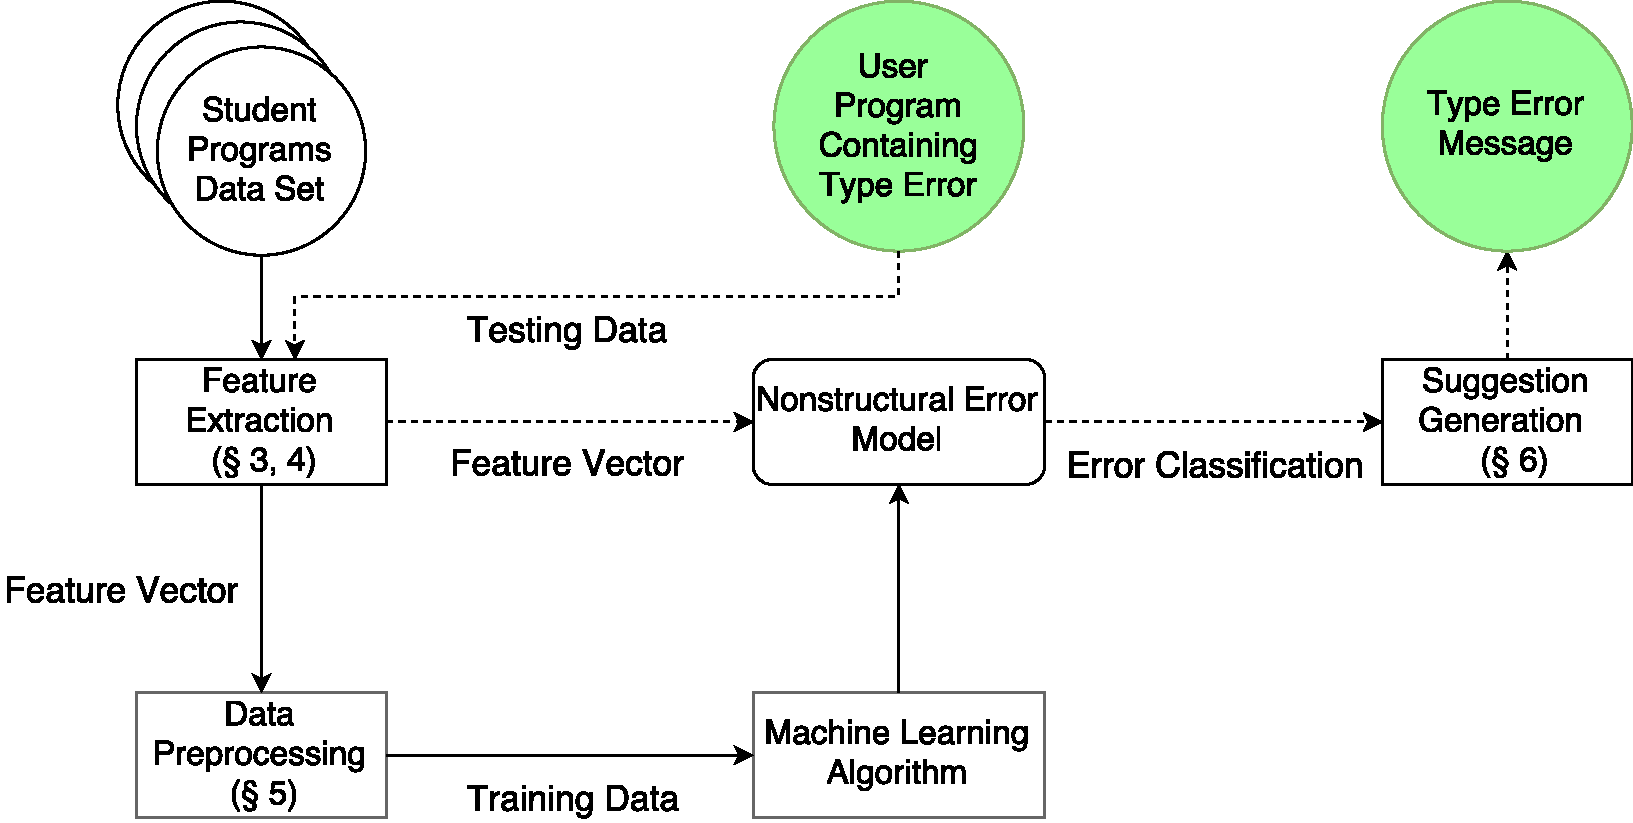
\includegraphics[scale=.85]{images/Learnskell.pdf}
\caption[The overview of \newCompiler]{The overview of \newCompiler. The circles denote the input
and output of the system. 
%Unfilled shapes and
%filled shapes denote the training and prediction
%processes, respectively.
The solid and dashed arrows
reflect information flow in the training and prediction
stages, respectively.
}
\label{fig:arch}
\end{figure}

\newCompiler\ produces the following message
for the \prog{groepeer} program shown in Chapter~\ref{sec:features}.
We have omitted
the information about the expected type and the inferred type.
%
\begin{program}
Add an open parenthesis before *drop* and a closing parenthesis after *x*
And needs some further changes
\end{program}
%
This message correctly diagnoses the nonstructural error and 
provides a concrete change suggestion to guide the user to fix
the type error. 


We justify the motivation for using ML in Section~\ref{sec:ml:motivation}.
In Section~\ref{sec:ml:back}, we review some concepts about
measuring the error rate of an ML model
and the bias-variance tradeoff.
In Section~\ref{sec:ml:prep}, we discuss
how to reduce the error rate by preprocessing our training data.
We resolve the
imbalanced classification problem
and use a cross-validation method to
select the appropriate ML algorithm in Section~\ref{sec:ml:smote-cv}.


\section{Motivation for Using Machine Learning}
\label{sec:ml:motivation}

The goal of \newCompiler\ is to produce
user-friendly type error messages for nonstructural errors.
We achieve it by adopting the idea of machine learning.
In this section, we discuss why machine learning
can help to make full use of error information for
nonstructural error determination.

We use the following expressions to illustrate the discussion in
this section.
%
\begin{program}
v1 = map (not True) [False]   
v2 = map True [False]   
v3 = let func = not True 
     in map func [False]
\end{program}
%
For \prog{v1}, the type error is caused by the subexpression \prog{not True},
with the expected type being \prog{a -> b} and the inferred type being \Bool.
While these two types are non-unifiable, we observe that the expected type
has two \emph{spine}s, \prog{a} and \prog{b}, and the inferred type has one
spine, \Bool. Intuitively, a spine is the domain of a top-level
arrow or the codomain of the last arrow at the top level. For example,
the type \prog{(a->b) -> [a] -> [b]} has three spines. A function with $n$
spines can be applied to $n-1$ arguments. Consequently, the fact that the
expected type has one more spine than that of the inferred type in \prog{v1}
indicates that the 
erroneous subexpression has been applied to 
an extra argument.
In other words, we may remove the type error by removing the
argument \prog{True}. Besides spine differences, bracket differences in
types also provide insights about how type errors may be fixed.

While type differences help to infer possible fixes, they alone
are insufficient. Consider, for example, the expressions \prog{v2}
and \prog{v3} below \prog{v1}. For both of them, the
expected type and the inferred type are exactly the same as those
for \prog{v1}. Inferring to remove an argument, as we did in \prog{v1},
is totally misleading. One can't remove an argument from \prog{True}
(the error cause in \prog{v2}) or \prog{func} (the error cause
in \prog{v3}). We can, however, address this issue by extracting
program structure information around the error cause.
For example, the location of the error cause in the program
AST helps us to decide whether ``Remove an argument'' is an appropriate
suggestion because we can't remove an argument if the error cause is a leaf.
Moreover, other kinds of program structure information
are also useful. For example, the fact that \prog{func} is a let-bound
variable indicates that the type error may be fixed by making
\prog{func} into a function if we view it as a 
point-free function~\cite{jones2003haskell}.

We may think of extracting all relevant information and
constructing changing rules manually. However, this
idea suffers from three shortcomings.
%
% First, the more information we extract, the
% better insights we may gain for diagnosing errors,
First, it's likely that if we extract more information we
can have better insights into diagnosing a given error.
Unfortunately, the dimension of feature vectors could be high
and similar errors can be represented by different feature
combinations. This hinders us in deciding what kind of
information is useful or not when constructing
changing rules for errors.
%
Second, it's very hard to come up with appropriate, consistent, and
coherent rules that make best use of extracted information.
%
For example, an error in a certain class
could have many variants. In practice it's likely
the rule we use to handle one error may not be able to handle its variants.
%
Finally, the generated suggestions lack statistical meaning,
yielding high ratio of misleading messages. For example,
while the suggestion of removing the argument \prog{True} to
\prog{not} in \prog{v1} fixes the type error, the suggestion
of changing the function \prog{not} (to, for example, \prog{const})
does so, too. The question is, which fix should we suggest?

All these problems could be solved nicely with machine learning.
The key idea is using
machine learning to construct
a model that can detect when type errors are likely
to be nonstructural.
This enables \newCompiler\ to find nonstructural errors and 
provide concrete change suggestions for them, 
in a way that is largely orthogonal to other debugging approaches.

\section{Preliminaries of Machine Learning}
\label{sec:ml:back}

In \newCompiler, we automatically extract a set of features
for a given type error. We use $\FE$ to represent this feature
extraction, which converts a type error $x$ into a finite feature
vector $v=\FE(x)$. The data set is denoted by
$D = \{(v_{1}, l_{1}), (v_{2}, l_{2}),...,(v_{i}, l_{i})\}$, where
$l_{i}$ is the label value of the error class for the
type error $x_{i}$.
The model $\M$ generated by an ML algorithm
can interpret the relationship between any pair of 
$v$ and $l$ in $D$.
%
The generalization
error $\varepsilon$ for the model $\M$ is estimated as follows~\cite{domingos2000unified}.
\begin{align*}
\varepsilon({\M}) &= \dfrac{1}{N}\sum_{i=1}^{N} P((v_i, p_i)\ |\ D) * L(l_i, p_i) \\
&= E[P((v, p)\ |\ D) * L(l, p)]
\end{align*}
%
We use $p=\M(v)$ to denote 
the prediction result produced by this model for any feature vector $v$ in $D$.
The loss function $L(l, p)$ is used to measure the cost of 
predicting $p$
with respect to the label value $l$.
For example, the zero-one loss function is commonly used in classification,
where $L(l, p) = 0$ if $ l = p$ and 1 otherwise.
%
\begin{definition}
Assume the number of all possible values of $l$ is $N_l$,
the optimal prediction for a feature vector $v$ is
$p_*(v) = \arg\min_{p'}E_{l}[L(l, p')]$, 
where $E_{l}[L(l, p')] = \dfrac{1}{N_l}\sum_{i=1}^{N_l} P(l_i\ |\ v) * L(l_i, p')$.
The model $\hat{\M}$ is optimal if $\hat{\M}(v) = p_*$ for every $v$.
\end{definition}

\begin{definition}
Assume the number of all possible values of $p$ is $N_p$,
the main prediction $p_m = \arg\min_{p'}E_{p}[L(p, p')]$,
where $E_{p}[L(p, p')] = \dfrac{1}{N_p}\sum_{i=1}^{N_p} P(p_i\ |\ D) * L(p_i, p')]$.
In other words, $p_m$ is the most frequent prediction generated by ${\M}$.
\end{definition}

We apply bias-variance decomposition \cite{domingos2000unified}
to $E[P((v, p)\ |\ D) * L(l, p)]$ and have:
\begin{align*}
\varepsilon({\M}) &= L(p_*, p_m) + c_1E[L(p, p_m)] + c_2E[L(l, p_*)]  \\
&= \it{Bias}(v) + c_1\Var(v) + c_2\it{Noise}(v) 
\end{align*}
%
The smaller the value of $\varepsilon({\M})$ is,
the better the ML model we obtain. 
The $\it{Bias}(v)$ denotes the systematic error of the model ${\M}$
by comparing with the optimal model $\hat{\M}$.
The $\Var(v)$ represents the fluctuations around the 
central tendency of prediction results with respect to data set $D$,
which is related to the precision of the classes.
The $\it{Noise}(v)$ is independent of the ML algorithm,
and it is usually unavoidable when estimating an ML model.


To minimize the error rate in ML model,
intuitively we shall minimize the bias and variance
in the model at the same time.
However, finding an optimal solution to minimize both bias and variance
is very hard.
The bias may be increased when reducing the variance, and vice versa.
This is called bias-variance tradeoff \cite{geman1992neural}.
For example, 
the variance is 0 in an ML model if 
this model always produces the same prediction result
regardless of the training data.
%
However, the bias in the model would be considerably large.
Such a situation in ML is called underfitting.
We can gradually increase the number of classes and 
eventually consider all type errors as
one class. By doing so, we minimize the bias in the model, while the variance
could be significant due to the large number of type error classes, 
which causes the ML model to overfit in this situation.

\section{Data Preprocessing}
\label{sec:ml:prep}

To evaluate whether an ML model is suitable to our application scenario,
it is desirable to have a program set containing both structural and nonstructural errors.
Moreover, it would be best to use a large data set with programs written
by novices.
This information enables ML to learn cues from various errors, which can
provide significant value to type error debugging.

There has been work collecting student programs to investigate how beginners learned
functional programming.
The study by \cite{hage2006mining} built a database with
over 60k student programs in Haskell.
While students were debugging errors,
each program that was
compiled with Helium was recorded.
This large program data set provides a sufficient amount of type errors for us
to construct the training data.
By comparing the ill-typed and well-typed versions of a student program,
we are able to find out how exactly a type error
was fixed in practice, which can be used to guide us
to label the class of each error in the training data.
We filtered out 1,604 ill-typed programs in year 2003-2004 from the program data set.
For every type error, we extracted the feature vector and manually labelled
its error class to construct our training data.
%
In this section we first use feature selection techniques to distill the extracted features,
and then we describe the strategy used to design the labels for different error classes.

In practice, most of the training data sets contain noise.
Moreover, the potential bugs in the implementation of feature extraction
and the possible mistakes in manually labelling data
could intensify the noise.
Reducing the noise is not trivial and most ML applications
consider it as irreducible error.
To reduce the value of $\it{Noise}(v)$,
we try to handle the data noise in the training data, to some extent.
We consider irrelevant and interdependent features as the noise, 
since removing these features
usually leads to a simpler and more flexible ML model.

In Section~\ref{sec:features:feature} we showed that there are more than 10
features extracted to represent the program structure around
the error location. Note that there  exists
dependencies among some features.
For example, feature 5 denotes what kind of expression the offending node is.
If the offending node is an operator, then we have feature 6 to describe
the associativity of the operator.
In addition, feature 7 shows the precedence of the offending node if
it is an operator.
Also, some feature values were redundant.
For example, if the offending element is an expression, then
its location in the AST is definitely at a node.
We want to examine whether these attributes are
relevant to the problem of type error debugging and
to identify how important they are.

To perform feature selection, we split
the training data into two sets.
We applied SGC classifier with $l_{1}$-norm \cite{Kearns:1994:ICL:200548}
to help us choose features on one set,
and we evaluated the ML model on the other.
%
Feature selection returns a subset of the relevant features
and importance ranking of all the features.
Incorporating our domain knowledge about nonstructural
errors and the understanding of the extracted features,
we can use the result of feature selection to decide
whether we should remove a feature.
For example,
we had a feature to keep track if the ill-typed
expression contained more than one identifier.
We found out that its feature importance was the smallest,
and we further realized that the feature was redundant since
its value can be inferred by the location of the error in AST
and the type of the offending node.
Therefore, it is safe to remove this feature.
In fact, the classification accuracy of our ML model
was improved by 4\% thanks to that removal.

We can also handle the data noise
by reducing the complexity of features.
It is possible that some features had many values,
but only one value was significant.
%
For example, initially we kept track if a function binding had syntactic sugar for lists 
in its parameters. We checked to see if some parameter was 
a list with a head and a tail
or if the function was point-free, etc. 
This created a large range of values
for this feature, which hurt the ML performance.
Eventually, we used a binary value to represent
whether a function definition was point-free or not only.
%though we still kept the information about parameter style for
%possible use in suggestion generation.

%variance
So far we have handled the data noise in the 
designed feature vector.
Next, we try to reduce the variance in the ML model.
\newCompiler\ focuses on handling nonstructural errors.
Accordingly, we first classify type errors into structural and nonstructural errors,
denoted by the error spaces $\X^{s}$ and $\X^{ns}$, respectively.
Since fixing nonstructural errors requires restructuring the AST by changing
parentheses or brackets, we further shatter $\X^{ns}$ in 4 sub-spaces,
namely "add brackets" as $\X^{ns}_{1}$, "remove brackets" as $\X^{ns}_{2}$,
"pull identifier from parentheses" as $\X^{ns}_{3}$,
and "merge identifiers" as $\X^{ns}_{4}$.
We can iteratively shatter each sub-space into another 2 new
sub-spaces. For example, the space $\X^{ns}_{3}$ can be
shattered in $\X^{ns}_{3_{1}}$(pull 1 identifier from parentheses), and
$\X^{ns}_{3_{>1}}$(pull more than 1 identifiers from parentheses).
Moreover, by combining rules from handling parentheses and brackets,
we could shatter a space in other sub-spaces 
like $\X^{ns}_{3\&1}$(pull identifier from parentheses \& add brackets),
and $\X^{ns}_{3\&2}$(pull identifier from parentheses \& remove brackets).
For these data spaces that introduce more than one change
to represent nonstructural errors,
we do not consider them.
This is because we can handle such errors by
several fixing steps.
%
Nevertheless,
some sub-spaces with only one change,
which have very few error cases,
could also be negligible.
For example, $\X^{ns}_{1_{4}}$ indicates adding 4 brackets to fix the nonstructural error,
while in practice this rarely happens.

So when should we stop shattering the space $\X^{ns}$ and which sub-spaces we should
assign labels to? Based on the concept of bias-variance tradeoff,
the variance in the ML model decreases while the bias increases
if we assign labels to the low dimensional spaces,
and vice versa if we assign labels to the high dimensional spaces. 
Our strategy is to reduce the value of $\Var(v)$ for the ML model first,
and then we reduce the bias by selecting 
the most appropriate ML algorithm after data preprocessing.
Therefore, we assign different labels to
the four error spaces $\X^{ns}_{i}$,
where $i \in [1,2,3,4]$.
Since changing the operator \prog{\$}
has the same effect of adding or removing 
parentheses, 
%and thus involves nonstructural changes, %hence
we created a label to represent such nonstructural error space $\X^{ns}_{s}$.
In Section~\ref{sec:ml:impl},
we discuss how our suggestion
generation algorithm determines the number of brackets needs to be changed
or the number of identifiers needs to be pulled/merged.

\section{Imbalanced Classification}
\label{sec:ml:smote-cv}

Most ML algorithms assume, by default, the data distribution of each class is balanced~\cite{he2009learning}.
During data labelling,
we found out the numbers of errors
in class $\X^{ns}_{4}$ and
$\X^{ns}_{s}$ are much smaller than other classes.
The distribution ratio of these minority classes is only around 6\%.
Conventional ML models usually fail to provide good prediction accuracy
across the classes when learning from imbalanced training data.
To deal with the imbalanced classification problem,
we can adopt a cost-sensitive
ML model or resample the data set.

Cost-sensitive methods~\cite{elkan2001foundations,ting2002instance} require a proper cost function
to describe the penalty for misclassifying any type error.
To achieve a good accuracy, we usually need to heavily tune the parameters
in the cost function. In addition, for different ML models, we need to use different
cost functions and repeating the tuning process.
% the corresponding function parameters again.
Such approaches aim to improve the efficiency of a certain
ML algorithm when having imbalanced data,
while our goal is to find an ML algorithm that provides the best classification accuracy.
Therefore, we do not use cost-sensitive methods to handle
the imbalanced classification problem in this work.

The essential idea of data resampling is to balance the 
given data set. This can be achieved with 
undersampling, which 
removes some existing data in the majority classes~\cite{liu2009exploratory},
or oversampling, 
which creates some new data in the minority classes~\cite{Chawla:2002:SSM:1622407.1622416,wang2004imbalanced,jo2004class}.
The resampling approach allows us to first
balance the training data and then
fairly evaluate the performance of different ML algorithms
in an efficient way.
Since we do not have an extremely large data set, applying undersampling
methods to our data set may filter out many useful error cases,
and consequently hurt the classification accuracy due to 
the underfitting problem.
A naive way to oversample the imbalanced data
is randomly replicating the records in the minority classes.
However, this would lead to the overfitting problem.

To properly synthesize new data in the minority classes,
the challenge is to make sure the generated data points
do not destroy the characteristics of the structures
of the original data set. Most of oversampling
methods address this challenging by inserting 
the synthesized
data point into an area of the imbalanced
data space such that the similarity distances
between the new point and its neighbours are
small. Thus, the measurement of 
the similarity distance
between two data points directly affects
the quality of the oversampled data set.

%
SMOTE~\cite{Chawla:2002:SSM:1622407.1622416} is a popular
data oversampling technique. In SMOTE, each
feature in the feature vector contributes to the calculation
of similarity distance. As a result, SMOTE works well when
all features are independent. 
%
However, there exists some dependency among
the features in our feature vector. For example, 
the values of both feature 7 and 8 are partially
dependent on the value of feature 5, as illustrated 
in Figure~\ref{fig:fvoverview}. Therefore, directly
applying SMOTE in our case may not work well since
the contributions of the interdependent features to the similarity
distance could be over-considered.
%
Instead of considering all features 
individually in computing the similarity distance,
we use the common vector, which is an
intersection of two feature vectors,
to measure the similarity distance between 
two feature vectors. 
Intuitively, two feature vectors that share 
a large common vector may have a small similarity
distance.
%the more similar two feature vectors are,
%the more number of features they should share.
We formally developed our distance metric 
%A new distance metric is proposed 
based on the idea of 
information entropy~\cite{shannon2001mathematical}
of common vectors.
We replaced the distance metric in SMOTE with our own distance metric.
We refer to this new approach SMOTE-CV.

\subsection{The Distance Measurement}
\label{sec:smotecv}

There are two general metrics called per-category
feature importance (PCF) and cross-category feature importance (CCF) that
can be used to measure the similarity distance between two data points \cite{creecy1992trading}.
% use N_{f} instead of \N_{f}. let's just curry the notaion of functions.
We use $N_{f}$ to denote the number of extracted features, and
$N_{c}$ denotes the number of different classes.
The basic PCF and CCF for two type error feature vectors, $u$ and $v$, are defined as:
\begin{align*}
PCF(u, v) &= \sum_{f}^{N_{f}}\omega(l_{u}, f) d(u_{f}, v_{f})\ \ \ \where\ \ \omega(l, f) = P(l\ |\ f) \\
CCF(u, v) &= \sum_{f}^{N_{f}}\omega(f) d(u_{f}, v_{f})\ \ \ \ \ \ \ \where\ \ \ \omega(f) = (\sum_{i=1}^{N_{c}}P(l_{i}\ |\ f)^2)^k \\
d(x, y) &= \left\{
							\begin{array}{lr}
							1\ \ \ \ \ \ifit\ x = y \\
							0\ \ \ \ \ \ifit\ x \neq y
							\end{array}
				\right.
\end{align*}

We can replace the distance function $d(x,y)$ with any other
function, or replace $\omega$ with any other weight metric
%use any other weight metric to replace $\omega$
to compute the similarity of $u$ and $v$.
For example, SMOTE uses a different $d$ and sets the parameter $k=0.5$
for $\omega$ to construct its own similarity metric.

Note that for most of the similarity metrics based on PCF/CCF, they
compute the contribution of each
individual feature to the
distance between two data point first, and
then combine the contributions of
all the features to generate the final result.
However, calculating the similarity by following this manner does not
work well in our case, since we have
lots of interdependent features.
For example, our features 6 and 7 are dependent
on feature 5. Both values of feature 6 and 7 would be -1
if the offending node in feature 5 is not an operator.
Therefore, using PCF/CCF-based methods
would over consider the similarity contribution from the interdependent features.
%
% I think this expression is wrong. Not what I mean.
%could consider the interdependent features overly similar.
%
As a result,
we proposed a new way to measure the similarity
distance for a data set with dependent features.

Intuitively, the more similar two feature vectors are,
the more number of features they should share.
We use $cv_{uv}$ to denote the common vector
between two feature vectors $u$ and $v$,
and we want to study
how much information of the similarity between
$u$ and $v$ that the $cv_{uv}$ can tell us.
We use entropy $\delta = log_{2}(\frac{1}{P(cv_{uv})})$
to represent such information, 
where $P(cv_{uv})$ is the probability that
the common vector $cv_{uv}$ exists among the feature vectors.
The entropy $\delta$ indicates that
infrequent common vectors convey more
information about the similarity than frequent common vectors.
For example, if $cv_{uv}$ appears more frequently in the feature vectors of
the same error class, then it is reasonable to
consider the two errors are less similar and vice versa.
Therefore, we define the similarity distance between
$u$ and $v$ within the class $q$ as:
\begin{align*}
\delta^{'}(u, v, q) &= H(cv_{uv}\ |\ q) \\
                      &= -\omega'log_{2}(\omega') - (1-\omega')log_{2}(1-\omega') \\
                      \where\ \ \omega' &= P(cv_{uv}\ |\ q)
\end{align*}

The entropy $\delta^{'}$
is similar to the usage of PCF, which
only considers the distance between two
errors within the same class.
The study by \cite{Mohri94anoptimal} showed that PCF is sensitive
to the distribution of classes.
Therefore, directly using $\delta^{'}$
as a distance measurement may not be appropriate
because of the imbalanced data in our application.
To address this issue, we
%prefer ( I do mean "refer to":) not prefer)
refer to the concept of CCF, which
tries to measure the similarity of two data points
across all the classes. Accordingly, we define
the new distance metric as
$\delta(u, v) = \sum_{i=1}^{N_{c}}P(q_{i})\delta^{'}(u, v, q_{i})$,
which averages $\delta^{'}$ over all the error classes.

We implemented a new oversampling method with the distance metric $\delta$, 
called SMOTE-CV, based on SMOTE.
We evaluated the performance of SMOTE-CV
by using random forest to classify the Year-03
program set. The result in Figure~\ref{fig:cse} 
shows that the performance for predicting
errors in imbalanced classes is improved by adopting oversampling techniques.
Although SMOTE outperforms than SMOTE-CV by about 1\% 
on the classification of structural errors,
SMOTE-CV yields better accuracy than SMOTE by about 6\%
when dealing with the minority classes like ``Pull''.

\begin{figure}
\centering
\setlength\tabcolsep{4pt}
  \begin{tabular}{  l | ccc | ccc | ccc }
\toprule
    \multirow{2}{*}{Error Class}
     & \multicolumn{3}{c|}{Precision} & \multicolumn{3}{c|}{Recall} & \multicolumn{3}{c}{$F_1$} \\
        & Base & SMO & SMO-CV &  Base & SMO & SMO-CV &  Base & SMO & SMO-CV\\ 
\midrule
    Delete Brackets & 0.769 & 0.773 & 0.807 & 0.671 & 0.731 & 0.819 & 0.800 & 0.740 & 0.804\\ 
    Merge & 0.858 & 0.824 & 0.853 & 0.925 & 0.944 & 0.906 & 0.887 & 0.878 & 0.873\\
    Pull & 0.875 & 0.825 & 0.930 & 0.510 & 0.570 & 0.625 & 0.623 & 0.662 & 0.715\\
    Add Brackets & 0.795 & 0.778 & 0.797 & 0.853 & 0.853 & 0.853 & 0.814 & 0.800 & 0.816\\
    Has \prog{\$} & 0.750 & 0.723 & 0.867 & 0.600 & 0.850 & 0.800 & 0.650 & 0.741 & 0.813 \\
    Structural & 0.847 & 0.895 & 0.883 & 0.868 & 0.850 & 0.851 & 0.856 & 0.871 & 0.866 \\
\bottomrule
  \end{tabular}
    \caption[A comparison of oversampling techniques]{A comparison of oversampling techniques. 
    We use the short names SMO and SMO-CV for SMOTE and SMOTE-CV, respectively.}
    \label{fig:cse}
\end{figure}


\subsection{Model Selection}
\label{sec:mlmodle}

With the features extracted in Section~\ref{sec:features:feature},
we use supervised learning to train a model for type error classification.
Four traditional machine learning algorithms are considered,
namely logistic regression~\cite{walker1967estimation}, 
Support Vector Machine (SVM)~\cite{cortes1995support}, 
decision tree~\cite{quinlan2014c4} and random forest~\cite{breiman2001random}.
%
We do not consider deep learning algorithms using neural networks as the classifier in \newCompiler\ for two reasons.
First, deep learning algorithms usually require vast amounts of training data to train the model, 
leading to a very low training speed.
Second, the training process of neural networks requires manually tuning the hyper-parameters,
which is tedious and hinders us from automating the error message generation.
%
In the next, We discuss the advantages and disadvantages of those evaluated supervised learning algorithms.

\parag{Logistic Regression}
%
Logistic regression~\cite{walker1967estimation} is similar to generalized linear model~\cite{mccullagh1984generalized},
which learns a linear boundary between classes.
It is simple, efficient and robust, and thus widely used in practice.
However, logistic regression does not work well for non-linear classification problems.

\parag{Support Vector Machine}
%
Support Vector Machine (SVM)~\cite{cortes1995support} is a supervised learning algorithm that builds
a model based on the training dataset to separate data into two classes
such that the gap between two classes is as wide as possible.

SVM is able to work efficiently in high dimensional spaces,
and it can learn non-linear boundary by using ``kernel trick''~\cite{mika1999fisher}.
%
The main limitation of SVM is the choice of kernel functions.
There are many kinds of kernels, such as Gaussian kernel, Fisher kernel, etc.
In practice, it is hard to determine which kernel works the 
best for a specific classification problem. 
As a result, using SVM usually requires considerable effort to tune the hyper-parameters.
We tested different kernel functions and found polynomial kernel with degree-2
yields the best result in our case.

\parag{Decision Tree}
%
The key idea of Decision Tree~\cite{quinlan2014c4} is to map
the feature vectors and the labels based on a tree structure.
The decision tree is constructed by recursively partitioning training data
until its impurity is minimized.
There are several metrics to measure the purity of the tree, such as entropy, gini index, etc.
A node in a decision tree is a single prediction of a certain feature $x_i$ such that
it can determine which subtree should be proceeded based on the value of $x_i$ of an input data.
Each leaf of the decision tree represents a class label.

Decision trees can work with little data and its predictions are easy
to understand and interpret.
However, the main drawback is that the learned model is often overfitting,
which means that the prediction precision may be poor 
in our case since the evaluated programs are diverse, coming from different students.

\parag{Random Forest}
%
Random Forest~\cite{breiman2001random} constructs multiple decision trees based on the training data
and uses the mean prediction of all trees as the final class.
By randomly sampling data from the training data,
different decision trees are learned from different data, 
which improves the model generality.
In addition, for each decision tree, a subset of features
is randomly selected for training such that the correlation between
learned trees is mitigated. 

Random forests can make accurate prediction efficiently, 
requiring little parameter tuning.
Therefore, it works very well across different application scenarios. 
The limitation of random forest is that it works as a black box, which 
makes prediction results hard to interpret.

\parag{Selection Result}
We used cross-validation~\cite{kohavi1995study} to evaluate the
performances of different ML algorithms based on the training data.
The average accuracy and standard deviation are
0.83 $\pm$ 0.08 for logistic regression,
0.64 $\pm$ 0.09 for SVM with a degree-2 polynomial kernel, 
0.83 $\pm$ 0.06 for SVM with a linear kernel, 
0.82 $\pm$ 0.08 for decision tree,
and 0.85 $\pm$ 0.07 for random forest with 100 trees.
%
Moreover, we tested random forest with 500 trees and 
did not observe any difference from random forest
with 100 trees. 
%
Since random forest yields the best performance over the others,
we use it as the model to predict nonstructural errors in this work.

\section{Implementation}
\label{sec:ml:impl}

We have implemented a prototype of \newCompiler\ using both Haskell and
Python. We used Haskell for implementing feature extraction and
suggestion generation. For each ill-typed program, we first call
Helium to get the relevant information, including the error
cause and the expected type and inferred type of the error cause. Note
that the location returned by Helium could be
very different from the location \newCompiler\ reports. For
example, for the \prog{groepeer} example in Chapter~\ref{sec:features},
Helium reports the error at \prog{groepeer} after \prog{++}, while our
approach reports it at \prog{drop n x}. Based on the information
returned by Helium, we apply the algorithms \ualg\ and \dalg\ from
Section~\ref{sec:unify:alg} to compute the type difference and
implement other functions to extract the features listed
in Section~\ref{sec:features:feature}.

We implemented SMOTE-CV in Python,
and it was used to resample the extracted feature vectors from the training data.
We fed the feature vectors to the \emph{scikit-learn} python package \cite{scikit-learn}, 
which generated the ML model for capturing nonstructural errors.
%
For any feature vector
of an ill-typed program, we provide it to the model, which will
generate the classification result. The result
includes two error classes, ordered by their corresponding probabilities.

For each class, we use the following rules to generate suggestions.
We collect all of the suggestions and select the first three.
If the type error is classified as a structural error,
we use the corresponding error message generated by Helium directly.
Otherwise, the suggestion generation module 
first checks the class of the
%
nonstructural error. 
For the class ``has \prog{\$}'', 
we simply suggest to remove \prog{\$} first. 
If the class is ``Merge''
or ``Pull'' (the meanings of them are defined
in Section~\ref{sec:ml:prep}), then only one message is
generated. In this case, the
indices of the first two elements in \FuncDiff\ (defined in
Section~\ref{sec:features:unify}) are used to
decide where to add the parentheses or pull
arguments and the number of arguments to change.
For example, for \prog{groepeer}, the class of the second type error is ``Merge''
and the values of \FuncDiff\ are 2 and 2, respectively, indicating that starting from the
second argument two arguments should be removed.
Therefore, we suggest adding parentheses over three arguments to fix the type error.
%is achieved by adding parentheses over three arguments.

If the class is ``Delete Brackets''
or ``Add Brackets'', then we generate three suggestions.
We generate more messages for dealing with bracket
differences because there are numerous possibilities for
fixing such errors while the fixing for parentheses
errors is quite certain. In this case,
the indices of the first two elements of
\BracketDiff\ are used to generate suggestions. We suggest
to change the expression specified by the first index, the
first identifier of the error cause, and the
parent node of the error cause. Of course, we may tune
these rules to achieve better precision, but we wanted
to keep change suggestions simple, given a classification result.

Sometimes the rule may fail to generate a suggestion with
the given nonstructural error class. 
The reason is either the
classification result is wrong, 
or the \FuncDiff\ / \BracketDiff\ is empty. 
One example is that
the predicted class is ``Pull''
but we don't have any expressions
nested in parentheses. 
In such cases, 
we follow the suggestions from Helium.

\section{Evaluation}
\label{sec:ml:eval}

To evaluate our work, we trained our model on the \trainset\
program set~\cite{Hage09:Neon}, which contains 1,604 ill-typed
programs. We evaluated the effectiveness of \newCompiler\
on the benchmark collected by \cite{Chen14:CFT} and the
\evalset\ program set. Since the first benchmark is
very small, we briefly discuss the result in
Section~\ref{sec:eval:sherrloc}. The \evalset\
contains 2,000 ill-typed
programs and we chose 1,000 programs from them randomly
for evaluation. Our evaluation focuses on this data set.
The programs in \trainset\ and \evalset\ were written by different
students in two different years. In these years, students worked
on different programming exercises and
assignments~\cite{Hage09:Neon}.


Each error message generated by \newCompiler\ consists
of three main parts: 
\begin{enumerate*}
\item the information indicates whether the type error is structural
or nonstructural (this information is not shown to the user since
it is not needed for fixing the type error),
\item the location of the type error in the program, and
\item a suggestion about how to remove the type error. 
\end{enumerate*}
%
We use the term ``accuracy'' when discussing the 
quality of ML classification and part (1) of messages, 
``precision'' when discussing the quality of part (2) 
of messages, and ``concreteness'' when taking about
the quality of part (3) of messages.

Our evaluation focuses on four aspects. 
In Subsection~\ref{sec:eval:model-accuracy}, we present
the accuracy of both machine learning classification
and error messages.
In Subsection~\ref{sec:eval:error-location},
we compare the error locating precision of \newCompiler\ with
GHC and Helium, and in Subsection~\ref{sec:eval:sherrloc}
we compare \newCompiler\ with SHErrLoc.
%
We do not compare \newCompiler\ with Seminal~\cite{Lerner07:STM}
because it works for OCaml only. 
%
As we showed in Section~\ref{sec:effectiveness} that more concrete error
messages tend to be more effective for students to
fix type errors, we evaluate the concreteness of
our error messages in Subsection~\ref{sec:eval:concreteness}.
Finally, in Subsection~\ref{sec:eval:performance}, we measure the
performance of \newCompiler\
by considering large programs containing multiple type errors.

\subsection{\newCompiler\ Accuracy}
\label{sec:eval:model-accuracy}

To evaluate the accuracy of our trained ML model and 
suggestion generation in \newCompiler,
we first need to determine the ground truth of the error class 
of every type error in
the testing data set. Similar to what we did in Section~\ref{sec:ml:prep}
for the training data set, we manually labeled each type error in the Year-02
program set, and used the label values to test against the evaluation results.
Based on our label values,
there are no type errors belonging to the "Has \prog{\$}" class in the testing data.

To measure the accuracy,
%we introduce the following metrics, namely precision (\pr),
%recall (\re) and $F_1$.
we introduce the metrics precision (\pr),
recall (\re), and $F_1$.
\begin{equation*}
\pr = \frac{\tp}{\tp+\fp}\ \ \ \ \ \ \ \  \ \ \
\re = \frac{\tp}{\tp+\fn}\ \ \ \ \ \ \ \ \ \ \ \
F_1 = 2 * \frac{\pr*\re}{\pr+\re}
\end{equation*}
%
Given a set of errors belonging to a certain class,
$\tp$ (true positive) represents the number of errors correctly predicted by our ML model
as belonging to the positive class, while
$\fp$ (false positive) is the number of errors misclassified by the ML model as belonging to the class.
Similar to the definition of $\tp$ and $\fp$,
$\tn$ (true negative) and $\fn$ (false negative) represent the number of errors
correctly and incorrectly predicted
by our ML model as not belonging to the class, respectively.
Therefore, given a type error,
the metric \pr\ is the probability that
our model determines the class of this error correctly.
The metric \re\ indicates the ratio of type errors in a class
our ML model can predict.
$F_1$ score is the harmonic mean of \pr\ and \re,
which is usually used to represent the overall classification
accuracy of ML models.


Figure~\ref{fig:sub4a} shows the number of type errors
in each class and the classification accuracy based on the testing data.
Our model computes the probability of every class that a given
type error belongs to, and we take the class with the highest
probability as the classification result of the model.
%
The accuracy of the ML model for capturing nonstructural 
errors is 80\% and that for capturing 
structural 
errors is 84\%.
%
The overall accuracy for all the 1,537 errors is about 82\%,
which means that 82\% of the time our ML model can correctly
determine whether a type error is structural or nonstructural.

\begin{figure}
\centering
\begin{tabular}{r | l | c | c  c  c}
\toprule
  \multicolumn{2}{c|}{Error Class} & \# of Errors & Precision & Recall & $F_1$  \\ 
\midrule
\multirow{5}{*}{Nonstuctural} 
&  Delete Brackets & 230 & 0.76 & 0.87 & 0.81 \\ 
&  Merge & 104 & 0.91 & 0.68 & 0.78 \\ 
&  Pull & 69 & 0.73 & 0.67 & 0.70 \\ 
&  Add Brackets & 304 & 0.81 & 0.86 & 0.83 \\ 
&  Overall & 707 & 0.80 & 0.82 & 0.80 \\
\midrule
  \multicolumn{2}{c|}{Structural} & 830 & 0.86 & 0.82 & 0.84 \\ 
\midrule
\multicolumn{2}{c|}{Overall} & 1,537 & 0.83 & 0.82 & 0.82 \\
\bottomrule
\end{tabular}
\caption{Accuracy of ML model}
\label{fig:sub4a}
\end{figure}


With the classification result generated by the ML model,
\newCompiler\ uses the first two error classes with the
highest probabilities to generate error messages.
Take the program \prog{groepeer} as an example.
The two most likely error classes and their
probabilities are ``Merge'' (0.68) and ``Structural'' (0.25).
Two error messages are generated based on the results.
The first one suggests to add a pair of 
parentheses in the ill-typed expression,
and the second one suggests to use Helium's message.
Therefore, by considering the first 3 error messages,
\newCompiler\ can achieve a higher classification
accuracy than the ML model does.

%
Figure~\ref{fig:sub4b} shows the
accuracy of \newCompiler\ for determining the classes of
type errors for 
the Year-02 program set.
About 88\% of the time \newCompiler\
can successfully identify the class of type errors.
Note that \newCompiler\ has higher missing rates in the ``Merge''
and ``Pull'' error classes.
There are two reasons.
First, the recall values of these two classes in Figure~\ref{fig:sub4a}
are small, which indicates that many of the errors in these classes were 
not covered by our ML model.
Second, we sometimes fail to generate suggestions for 
errors in these two classes.

\begin{figure}
\centering
\begin{tabular}{ r| l | c  c  c }
\toprule
  \multicolumn{2}{c|}{Error Class} & Precision & Recall & $F_1$  \\ 
\midrule
\multirow{5}{*}{Nonstructural}
&  Delete Brackets & 0.81 & 0.93 & 0.87 \\ 
&  Merge & 0.93 & 0.71 & 0.81 \\ 
&  Pull & 0.80 & 0.70 & 0.75 \\ 
&  Add Brackets & 0.85 & 0.96 & 0.90 \\ 
&  Overall & 0.84 & 0.89 & 0.86 \\
\midrule
\multicolumn{2}{c|}{Structural} & 0.92 & 0.88 & 0.89 \\ 
\midrule
\multicolumn{2}{c|}{Overall} & 0.88 & 0.88 & 0.88 \\
\bottomrule
\end{tabular}
\caption{Accuracy of \newCompiler}
\label{fig:sub4b}
\end{figure}

\subsection{Precision comparison with GHC and Helium}
\label{sec:eval:error-location}

In this subsection, we compare the error 
locating precision 
of \newCompiler\ with Helium and GHC
for the ill-typed
programs in the Year-02 data set.
%
We say a message is precise if it locates the
type error correctly, matching the 
place where students changed to fix the type 
error. For example, based on how students 
fixed the type error in \prog{groepeer}~\cite{Hage09:Neon}, 
the message from \newCompiler\ is  precise
while those from GHC and Helium are imprecise.

Figure~\ref{fig:sub5a} shows the precision of locating nonstructural errors 
of \newCompiler,
with one change suggestion,
is 63\%, 
while those of Helium and GHC are 33\% and 21\%, respectively.
%the first suggestion,
%\newCompiler\ has twice the accuracy of
%Helium and thrice the accuracy of GHC.
The precision of \newCompiler\ rises to 74\% if
we consider the first two change suggestions 
and to 87\% if
we consider the first three. 
Helium and GHC can only generate
one message for each type error.
%
The overall error locating
precision of
\newCompiler\ showed in Figure~\ref{fig:sub5a} 
is quite good compared to other tools.
It achieves
almost twice the precision of GHC and
performs better than Helium. When considering
3 suggestions, \newCompiler\
is the only tool achieving a precision higher than 50\%.

\begin{figure}
\centering
\begin{tabularx}{.75\textwidth}{c *{5}{|Y}}
\toprule
\multicolumn{1}{c|}{} 
 & \multicolumn{3}{c|}{\newCompiler\ with \#\ of\ Sugg.}
 & \multicolumn{1}{c|}{}
 & \multicolumn{1}{c}{}\\
 Class & 1 & 2 & 3 & Helium & GHC \\
\midrule
Nonstructural & 0.63 & 0.74 & 0.87 & 0.33 & 0.21\\
Overall & 0.41 & 0.47 & 0.54 & 0.44 & 0.23\\ 
\bottomrule
\end{tabularx}
\caption{Precision comparison with GHC and Helium}
\label{fig:sub5a}
\end{figure}

In Figure~\ref{fig:Distance}, 
we compare \newCompiler\ with Helium and GHC to
see how frequently nonstructural errors of different classes
can be precisely located.
The result shows that \newCompiler\
outperforms Helium and GHC in every error class,
even when only considering the first change suggestion.
%
\newCompiler\ located the error causes for the
errors involving parentheses changes more
than 90\% of the time. For errors involving
bracket changes, 
about 60\% of the time the first suggestion of \newCompiler\
correctly locates the error causes.
When considering 3 suggestions, \newCompiler\ correctly
finds the real error location 
for each class more than 80\% of the time.

\begin{figure}
\centering
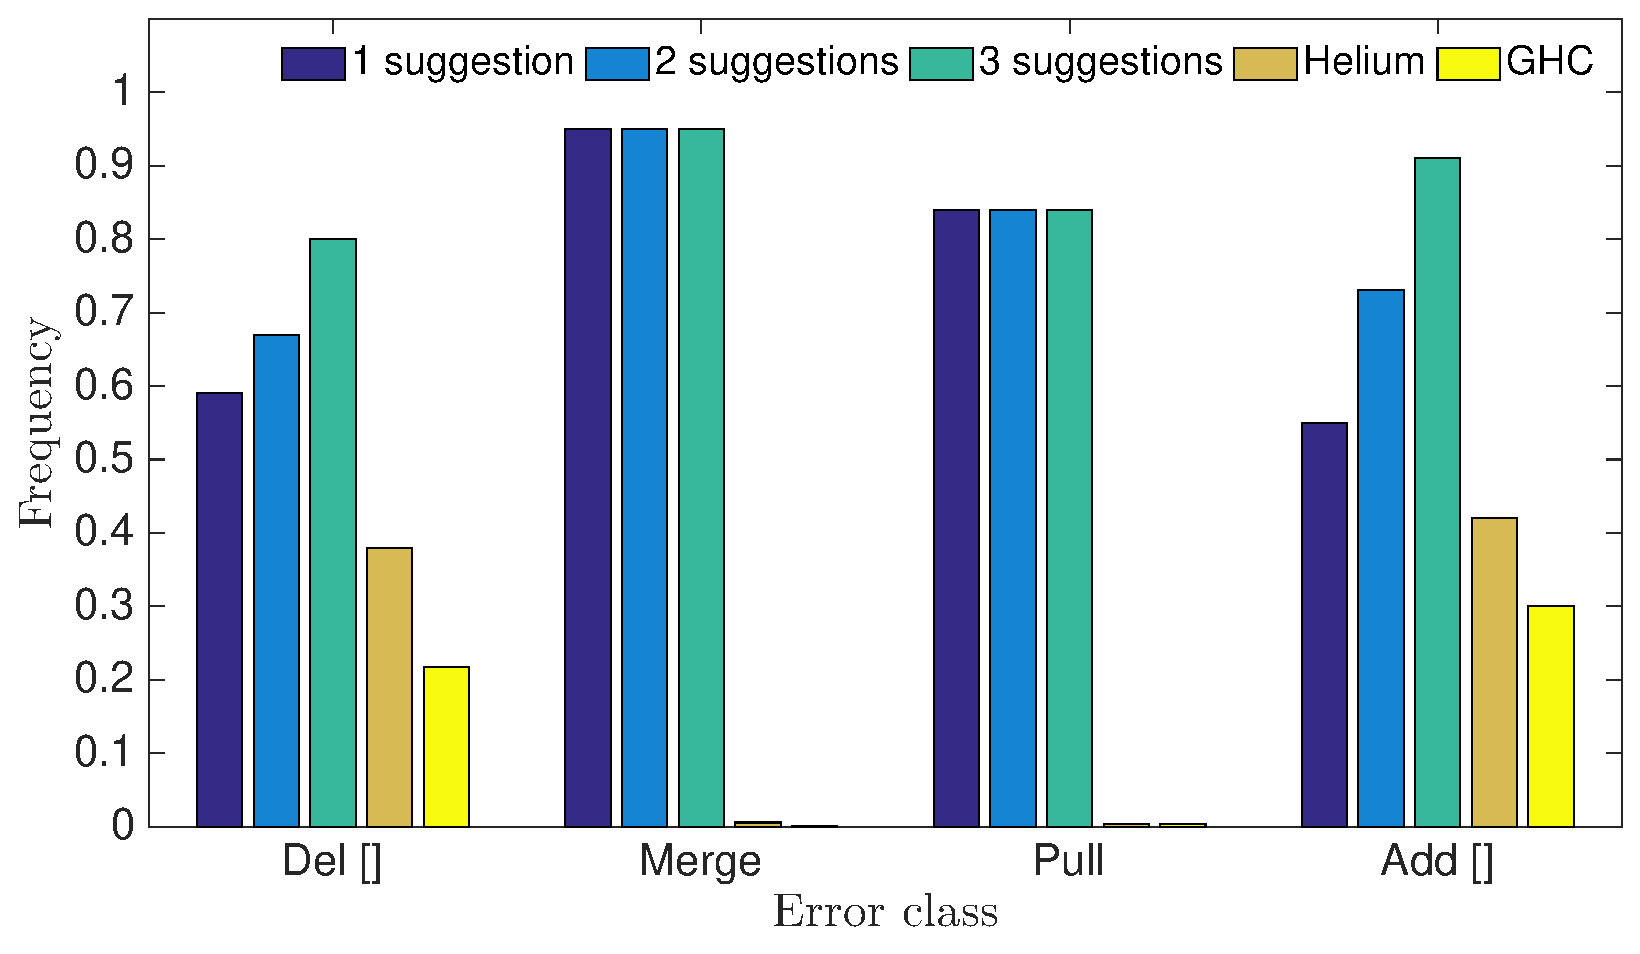
\includegraphics[width=.9\linewidth]{images/dist.eps}
\caption{Localization precision for nonstructural errors}
\label{fig:Distance}
\end{figure}

\subsection{Precision comparison with SHErrLoc}
\label{sec:eval:sherrloc}

SHErrLoc is a state-of-the-art type error debugger
that  locates error causes quite well. Consequently,
we are interested to evaluate \newCompiler\ against it.
SHErrLoc provides an off-line tool for Ocaml,
while there is only a web interface for compiling Haskell programs.
Therefore, we lacked an easy way to automate
the compilation process on a large program set.
%we lacked an easy way to automate
%parts of the evaluation process, due to using SHErrLoc's web interface.
In this evaluation, we randomly chose 186 programs
containing nonstructural errors from Year-02 data set.
%
For each type error, we considered the first three error 
messages presented by SHErrLoc, leading to a fair comparison 
of \newCompiler\ and SHErrLoc.

Figure~\ref{fig:SHErr} measures the precision of 
locations reported in messages, similar to Figure~\ref{fig:sub5a}.
Although SHErrLoc performs well in handling nonstructural errors
compared to Helium and GHC,
\newCompiler\
outperforms it by more than 20\%, 
considering the first
suggestion of \newCompiler.
With the first
three suggestions, the precision of \newCompiler\ increases to 82\%.
This shows that \newCompiler\ addresses
the nonstructural problem better than other
leading tools.

\begin{figure}
\centering
\begin{tabularx}{\textwidth}{c *{3}{|>{\hsize=.32\hsize}Y} |Y *{2}{|>{\hsize=.3\hsize}Y}}
\toprule
\multicolumn{1}{c|}{} 
 & \multicolumn{3}{c|}{\newCompiler\ with \#\ of\ Sugg.}
 & \multicolumn{1}{c|}{}
 & \multicolumn{1}{c|}{}
 & \multicolumn{1}{c}{}\\
 Class & 1 & 2 & 3 & SHErrLoc with 3 Sugg. & Helium & GHC \\
\midrule
Nonstructural & 0.69 & 0.76  & 0.82 & 0.47 & 0.22 & 0.13\\ 
Structural & - & - & - & 0.65 & 0.51 & 0.21 \\ 
\midrule
\end{tabularx}
\caption{\newCompiler\ precision with SHErrLoc, Helium and GHC}
\label{fig:SHErr}
\end{figure}


In Figure~\ref{fig:SHErr}, we also present the results
dealing with 86 programs that contain structural errors only.
%
Since all these type errors are structural,
\newCompiler\ did not generate any message.
As a result,
the entries for the suggestion categories are left empty.
We found out that SHErrLoc performed much better than Helium and GHC
when locating the real error cause for structural errors.
\newCompiler\ and SHErrLoc are strong in different cases,
therefore, combining SHErrLoc and our machine learning approach
may achieve a better overall precision.


The benchmark from \cite{Chen14:CFT} contains 10 nonstructural errors.
For them, \newCompiler\ precisely located 8 errors with the first message
and 9 with the first three messages, while SHErrLoc located only
3 of them with the first three messages.

\subsection{Suggestion Concreteness}
\label{sec:eval:concreteness}

To measure the concreteness of error messages,
based on the information error messages include,
we classify them into 4 categories,
namely \emph{\location}, \emph{\reason},
\emph{\correct}, and \emph{\concrete}.
\Location\ messages only report
the location and inconsistent types,
which are also contained in the error messages
of the other 3 categories.
\Reason\ messages explain why the type error occurred.
\Correct\ messages give a suggestion about
how a user could debug the error without a concrete expression.
\Concrete\ messages provide the expression-level
changes that fix the ill-type program.
We showed in Section~\ref{sec:effectiveness} that more
concrete messages tend to be more effective for users
to exploit to fix type errors. 

In this work, \newCompiler\ focuses on generating
\correct\ or \concrete\ messages for nonstructural errors,
while only providing \location\ messages for structural errors.
However, Helium can provide \reason, \correct, or \concrete\
messages for structural errors.
Therefore, a simple strategy for our tool to provide
more concrete error messages 
%for all the errors 
is combining \newCompiler\ and Helium.
If \newCompiler\ classifies a type error as structural,
then we present the error message from Helium to users.
Otherwise, we show the error message generated by \newCompiler.

\begin{figure}
\centering
\begin{subfigure}[t]{0.85\textwidth}
	\centering
    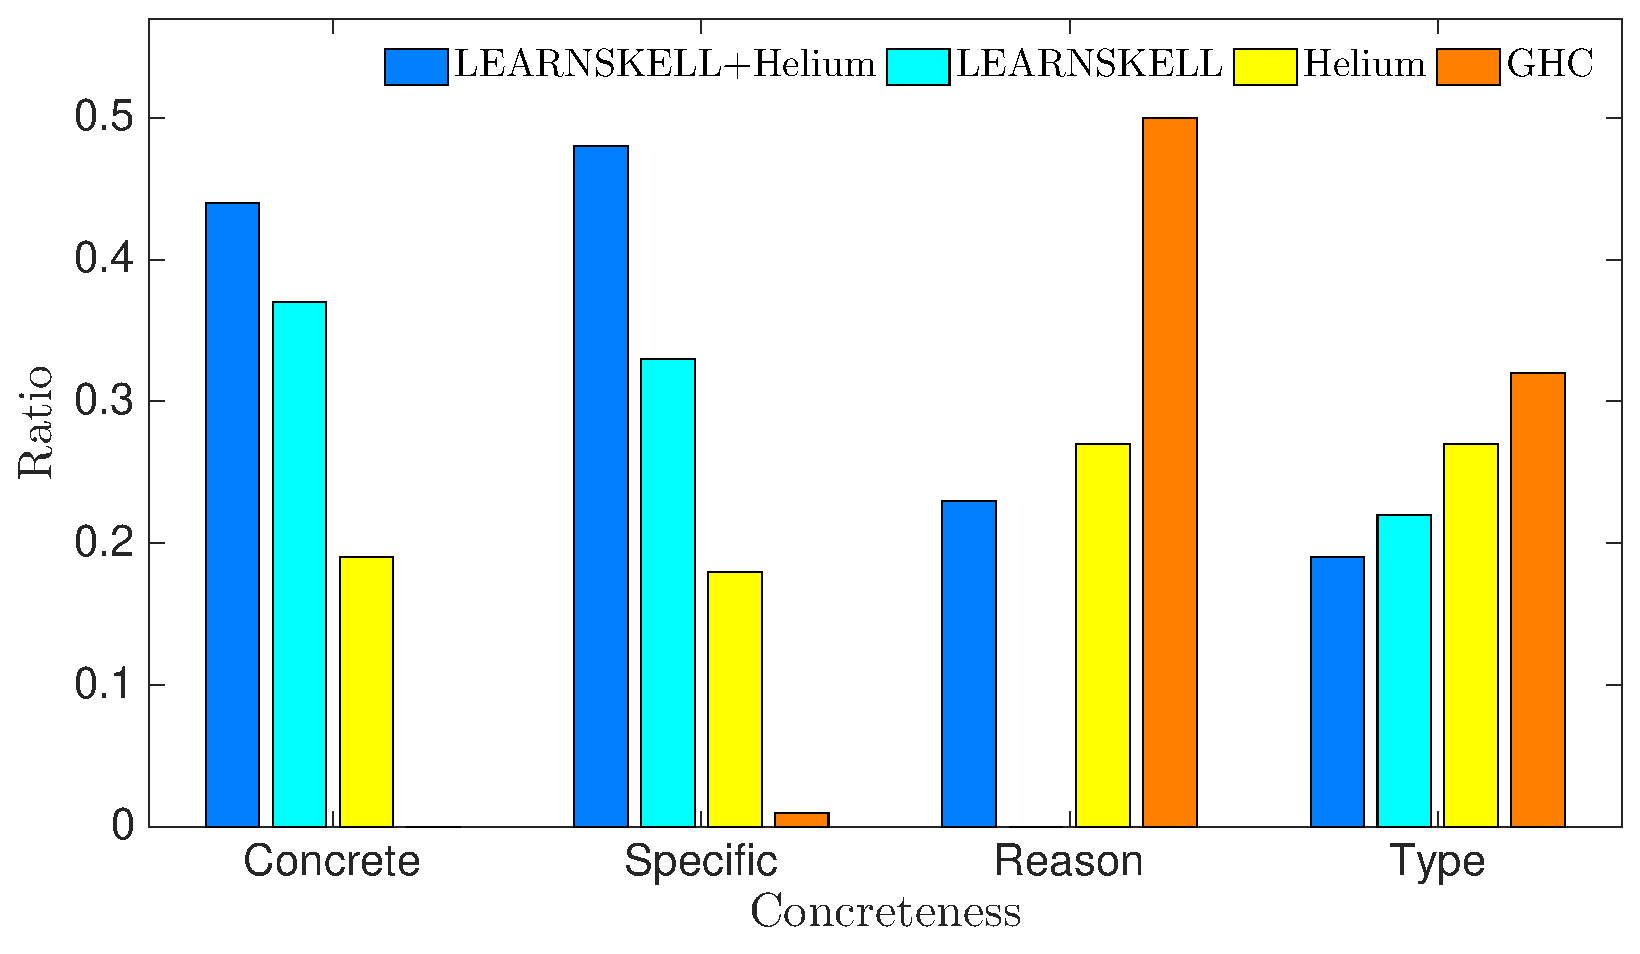
\includegraphics[width=.95\linewidth]{images/concrete_ratio.eps}
    \caption{Concreteness ratio}
     \label{fig:sub6a}
\end{subfigure}

\begin{subfigure}[t]{0.85\textwidth}
	\centering
    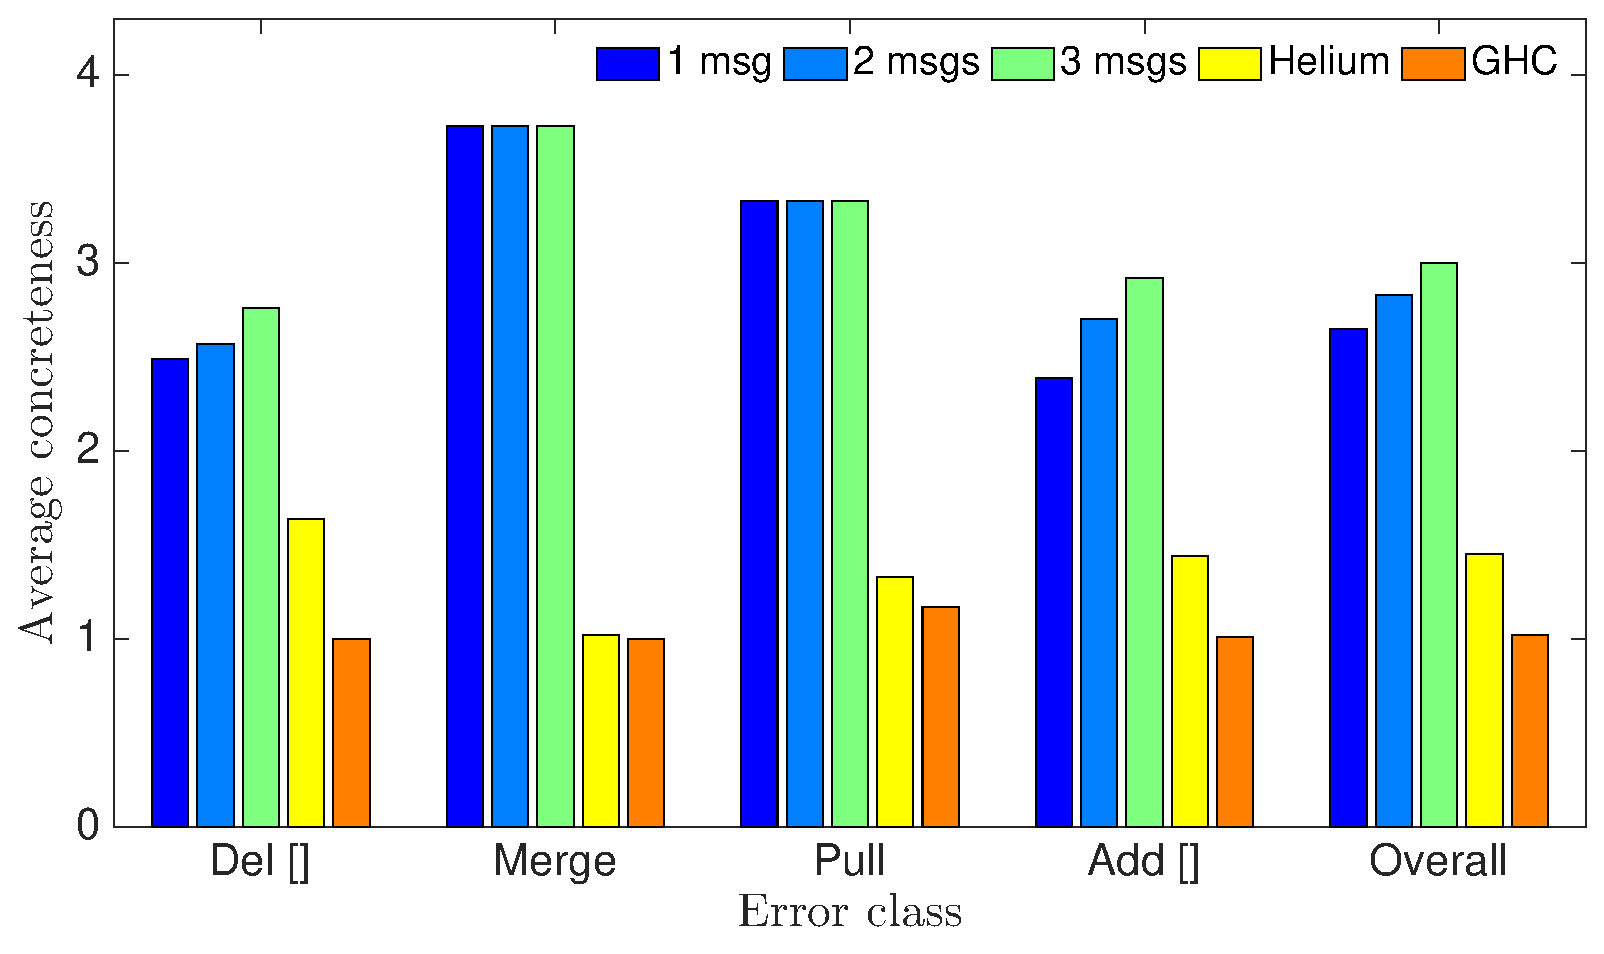
\includegraphics[width=.95\linewidth]{images/concrete.eps}
    \caption{Concreteness level}
    \label{fig:sub6b}
\end{subfigure}
\caption{Concreteness of error messages}
\label{fig:Concrete}
\end{figure}

Figure~\ref{fig:sub6a} shows the evaluation result of the concreteness of error messages.
%for all kinds of errors.
The value of y-axis represents 
the ratio of messages generated by different tools within a certain kind of suggestion.
In Figure~\ref{fig:sub6a},
the standalone \newCompiler\  generates \correct\
and \concrete\ suggestions more often
than Helium and GHC do.
In addition, by combining \newCompiler\ and Helium, 
we produce more \correct\ and \concrete\ error messages, 
which makes a more helpful tool for error debugging.

We assign a value 1 through 4 to each message if it is
\location, \reason, \correct, or \concrete, respectively,
that is we assign higher values to more concrete messages.
We compute the average concreteness of the messages generated
by a tool to give an intuitive idea about which message category 
it tends to generate.
%
Figure~\ref{fig:sub6b} presents the concreteness
result of different tools for handling nonstructural errors.
%
For each error class, the average concreteness of GHC and
Helium is between 1 and 2,
meaning that they largely provide \location\ messages
for all nonstructural errors.
For the nonstructural errors involving
parentheses changes,
the error messages provided by \newCompiler\ 
are almost entirely \correct\ and \concrete.
For the other error classes,
\newCompiler\ reaches an average value of 3
when three messages are considered.
The results show that, for different class of nonstructural errors,
\newCompiler\ can generate more concrete change suggestions
than Helium and GHC do.

\subsection{\newCompiler\ Performance}
\label{sec:eval:performance}

\begin{figure}
\centering
\setlength\tabcolsep{4pt}
  \begin{tabular}{  l | ccc | ccc | ccc }
\toprule
    & \multicolumn{3}{c|}{10 Errors} & \multicolumn{3}{c|}{20 Errors} & \multicolumn{3}{c}{40 Errors} \\
LOC & Extraction & Sugg. & Helium &  Extraction & Sugg. & Helium &  Extraction & Sugg. & Helium\\ 
\midrule
    100 & 0.006 & 0.008 & 1.234 & 0.012 & 0.016 & 2.496 & 0.026 & 0.031 & 4.895\\ 
    500 & 0.006 & 0.008 & 2.496 & 0.012 & 0.016 & 3.919 & 0.025 & 0.031 & 6.104\\ 
    1,000 & 0.006 & 0.008 & 4.732 & 0.013 & 0.016 & 5.427 & 0.026 & 0.033 & 8.542\\ 
\bottomrule
\end{tabular}
\caption[Running time of \newCompiler]{Running time of \newCompiler\ in seconds. 
Each time is an average
of 10 runs. Times are measured on
%
a laptop
with 4 GB of RAM and an AMD A6-3400M
quad-core processor running 
64 bit Fedora 23 and GHC 7.8.
}
\label{fig:LearnSpeed}
\end{figure}

The precision and concreteness
of type error messages diminishes
in value if error messages
arrive too slowly. Users prize
quick feedback when debugging type errors,
and they will be less likely to continue using
an error debugger if it takes a long time
to provide error messages in practice.
Therefore, scalability is an important factor to consider. 
We tested the efficiency of \newCompiler,
and show the results in Figure \ref{fig:LearnSpeed} by evaluating
the extraction time and suggestion generation time on
programs as large as 1,000 LOC, containing multiple nonstructural
and structural errors. Each program contains the same number
of nonstructural errors and structural errors. 
%
Suggestion generation always takes
similar time, regardless of the number of lines of code.
%
The Helium column in Figure ~\ref{fig:LearnSpeed} is the duration
our implementation (that is built on
%
Helium) ran for code that was not part of feature extraction and suggestion
generation. 
%
The
time Helium took increased with the number of lines of code,
as well as the number of errors.

The training time for
the ML model took around 3
minutes. This is of little
impact since it is a one-time cost.
The error classification time
is usually under 0.01 seconds, 
which is similarly of
little overhead, as with
feature extraction and
suggestion generation.
These results show that the
overhead in adding feature extraction and suggestion generation code into
a type error debugger is small. 
As a result, the approach used by \newCompiler\
is scalable, making it a practical design for
a type error debugger intended to work on large applications.

\chapter{Learning Precise Error Specifications}
\label{sec:app}


Besides debugging type errors, there are many other research directions in error debugging.
%
Error handling bugs are prevalent in libraries, system software, and
applications, and they often yield severe consequences, such as
security vulnerabilities~\cite{OWASP2007}.
%
Many methods have been developed to detect
error handling bugs. 
%
For example, \cite{Rubio-Gonzalez:2009:EPA:1542476.1542506} leverage weighted pushdown systems to analyze error propagation in file systems
for finding such bugs.
A set of dynamic analysis approaches, based on error injection, have also been developed 
to test if the binary code handles
failures correctly~\cite{marinescu2011efficient,susskraut2006automatically,gunawi2008eio}.
%
Each of these approaches~\cite{jana2016automatically,Rubio-Gonzalez:2009:EPA:1542476.1542506,gunawi2008eio} 
has detected hundreds of error handling bugs in their respective study subjects.

To illustrate, consider the code snippet in Figure~\ref{fig:errhandlingbug},
which shows how a bug detection tool, such as  EPEx~\cite{jana2016automatically},
is able to detect a bug
in the Linux kernel (versions before 4.20.15) 
that causes a security vulnerability (CVE-2019-12818~\cite{CVE:2019:12818}).
%
The bug is related to 
Logical Link Control Protocol (LLCP) and is in the NFC subsystem.
%
Note that, as line 17 shows, \prog{nfc\_llcp\_build\_tlv()} returns \prog{NULL} when a memory allocation fails (line 16) 
and no memory address is returned.
As a result, the error specification for \prog{nfc\_llcp\_build\_tlv()} is
\{\prog{NULL}\}. 
%
The function \prog{nfc\_llcp\_build\_gb()} 
calls \prog{nfc\_llcp\_build\_tlv()}
to allocate a block of memory for an NFC data exchange message (line 5).
%
It directly uses the returned memory on line 7, ignoring the
fact that the memory address could be \prog{NULL}.
This may 
trigger a NULL pointer dereference,
causing a denial of service failure.
%
To determine if the call 
to \prog{nfc\_llcp\_build\_tlv()} (line 5)
leads to error handling bugs,
EPEx examines whether the return value (\prog{lto\_tlv})
is properly checked against the corresponding error value (\set{\prog{NULL}}).
%
%EPEx can determine whether the call 
%to \prog{nfc\_llcp\_build\_tlv()} (line 5)
%leads to error handling bugs by checking its 
%return value (\prog{lto\_tlv}) against its 
%error specification, which
%is \set{\prog{NULL}}. 
%
Since such a check is missing, 
EPEx may report an error handling bug. 

\begin{figure}[t]
\centering
\begin{subfigure}[b]{0.5\textwidth}
\begin{Verbatim}[numbers=left,xleftmargin=6mm,fontsize=\footnotesize,
    commandchars=\\\{\}]
\it{/* Linux-4.19/llcp\_core.c */}
static int nfc\_llcp\_build\_gb (...)
\{
  ...
  lto\_tlv = nfc\_llcp\_build\_tlv(...);
  ...
  memcpy(gb\_cur, lto\_tlv, lto\_length);
  gb\_cur += lto\_length;
  ...
\}
\end{Verbatim}
\end{subfigure}%
\hfill
\begin{subfigure}[b]{0.5\textwidth}
\begin{Verbatim}[numbers=left,xleftmargin=6mm,fontsize=\footnotesize,
    commandchars=\\\{\},firstnumber=last]
\it{/* Linux-4.19/llcp\_commands.c */}
u8 *nfc\_llcp\_build\_tlv (...)
\{
  ...
  tlv = kzalloc(...);
  if (tlv == NULL)
    return \errline{tlv};
  ...
  return \correctline{tlv};
\}
\end{Verbatim}
\end{subfigure}
\caption[An example of an error handling bug]{An example of an error handling bug.
Function \prog{nfc\_llcp\_build\_tlv()} returns NULL on error (marked in italic-red)
and the start address of the allocated memory (marked in bold-green) on success.}
\label{fig:errhandlingbug}
\end{figure}

As shown in Figure~\ref{fig:errhandlingbug}, an important kind of information those methods rely on is
error specifications, which specify the value range each function
returns to indicate errors.
%
An example error specification is given in Figure~\ref{fig:errspec}.
The function \prog{deflatePrime()} from zlib 
tries to insert bits in a given stream \prog{strm},
but may fail in two cases.
%
When failures happen,
it will return \prog{Z\_STREAM\_ERROR} to indicate an inconsistent stream state
or \prog{Z\_BUF\_ERROR} to indicate that the stream does not have enough buffer to insert the bits.
%
Since zlib sets the values of the two macros \prog{Z\_STREAM\_ERROR} and \prog{Z\_BUF\_ERROR}
to -2 and -5, respectively, the error specification for \prog{deflatePrime()} is \{-2, -5\}.

\begin{figure}[t]
\begin{Verbatim}[numbers=left,xleftmargin=6mm,fontsize=\footnotesize,
    commandchars=\\\{\}]
\it{/* zlib-1.2.11/deflate.c */}
int ZEXPORT deflatePrime (
  z\_streamp strm, int bits, int value)
\{
  deflate\_state *s;
  int put;

  if (deflateStateCheck(strm))
    return \errline{Z\_STREAM\_ERROR};

  s = strm->state;
  if ((Bytef *)(s->d\_buf) < ...)
    return \errline{Z\_BUF\_ERROR};
  ...
  return \correctline{Z\_OK};
\}
\end{Verbatim}
\caption[An example error specification]{An example error specification.
The function \prog{deflatePrime()} returns 
\prog{Z\_STREAM\_ERROR} and \prog{Z\_BUF\_ERROR} on error (marked in italic-red)
while returns \prog{Z\_OK} on success (marked in bold-green).
}
\label{fig:errspec}
\end{figure}

%
Automatically generating precise error specifications 
is non-trivial in practice for several reasons.
%
First, 
while some conventions, such as
NULL pointers and negative values, are used in projects to denote errors,
they do not always hold.
This is because error values indicating failure are function-specific and 
may overlap with non-error values from other functions within
the same project. 
%within in the same project.
For example, in zlib, the function
\prog{gzgets()} uses a
\prog{NULL} to denote that reading a compressed file fails
whereas \prog{gzerror()}
returns a \prog{NULL} to indicate a compressed file stream is correct.
%
According to \cite{Kang:2016:AAI:2970276.2970354}, 
the precision
of error specifications collected following such 
conventions is only about 50\%. 
%
Second, in addition to such conventions, 
projects usually introduce their own idioms for representing errors.
%
For example, while OpenSSL uses \prog{SSL\_R\_UNSUPPORTED\_OPTION} to indicate errors,
Linux never uses this name.
As a result, identifying errors by pattern matching over a set of idioms does not work across projects.

In this chapter, we generate error specifications 
by first identifying error paths and then collecting
return values for these paths. 
A path is an 
\emph{error path} if its execution 
ends in error situations, 
for example, failing to open files, obtain resources, and allocate memory.
%
For instance, in the function \prog{nfc\_llcp\_build\_tlv} (Figure~\ref{fig:errhandlingbug}), the path that failed to allocate
memory (ends in line 17) is an error path and the path that obtained memory
(ends in line 19) is a non-error path. 

The key observation in our solution is that we can characterize paths
%from non-error paths
%(paths represent normal program executions)
through a set of features, such as path lengths
(the distances between the exit points and the corresponding entry points),
categories of return expressions (constants, variables, macros, etc.),
and the number of function calls involved along a path.
%
These features are related to the behaviors of programs, 
and are thus useful to identify \emph{error paths}.
%(path executions end in error situations such as failing to open files, to obtain resources, and to allocate memory).
For example, since error values in C are often returned by using ``goto'' statements~\cite{Nagappan:2015:ESG:2786805.2786834},
error paths are likely to have fewer number of function calls and/or branching points than non-error paths.


Based on path features, one straightforward way to identify error paths is
to employ some heuristics.
In APEx~\cite{Kang:2016:AAI:2970276.2970354},
the paths with fewer branching points and program statements than average are identified as error paths.
However, the accuracy of error path identification in heuristic-based approaches 
is low.
%NOTE: i change it back to 'is poor' since saying 'has room for improvement' may make our work seem incremental....
%has room for improvement. 
For example, 
the F-measure\footnote{
We measure the error specification accuracy by using the metrics precision,
recall, and \accu. We give the formal definitions of these metrics in Section~\ref{sec:app:eval:phase2}.
The \accu\ is a measure of the overall accuracy by computing the harmonic mean of precision and recall.} 
of APEx is only about 77\%.
The main reason is that the heuristic used in APEx only leverages two features, 
which is not comprehensive enough to cover different kinds of error paths.
%the number of features leveraged by the heuristic in APEx is too small.
To improve the accuracy, one can design a more sophisticated 
heuristic considering more features.
Ideally, a heuristic that appropriately, consistently, and coherently 
makes full use of all possible features could 
identify error paths with very high accuracy.
On the other hand, manually designing such heuristics is not feasible in practice 
when too many features are involved. 
Moreover, the identified error paths based on heuristics lack statistical guarantees, 
which means that the proposed heuristic may not generalize across different projects.
For example, APEx achieves 94\% F-measure for GTK+ while only 23\% F-measure for zlib.


To address these issues, we propose a machine learning-based method, named \newTool,
which effectively establishes a statistical relationship between the features and error paths. 
One inherent problem of traditional machine learning methods is that 
considerable manual data labeling efforts are required for training a model.
We build upon a simple insight that enables \newTool\ to move 
beyond such a supervised paradigm:
%and thus eliminate the needs for arduous labeling overhead:
although the paths in different projects exhibit distinctive properties 
%(described by project-specific features)
due to coding style, functionality, etc.,
%for example the functions invoked by the paths in zlib may not be the same as those in OpenSSL,
they share commonalities across projects. 
For example,
one common feature to characterize paths could be path length,
even though the functions invoked by paths vary from one project to another.
%
It is thus possible that the knowledge,
in terms of the common characteristics of error and non-error paths,
could be transferred from a pre-labeled project
to another project that has no labeled paths.
%
Based on the transferred knowledge, we learn
a ``tailored'' model for the unlabeled project,
eliminating the needs for arduous labeling overhead.

We formalize this intuition by proposing a novel two-phase learning approach 
and present its workflow in Figure~\ref{fig:workflow}.
%
In the first phase, 
transfer learning technique~\cite{pan2010survey} is introduced
to help transfer the knowledge from a pre-labeled project
to a new project without its label information, 
yielding a core model.
The core model 
samples a set of the most likely error and non-error paths.
%
%These paths are in turn used 
They are then used
as the training data set (since the set
is the output of the first learning phase,
% in the first phase, 
we refer to it as the \emph{learned training set} 
hereafter) in the second phase,
where a project-specific model is trained
to classify all paths as error or non-error in the new project.

\begin{figure}[t]
\centering
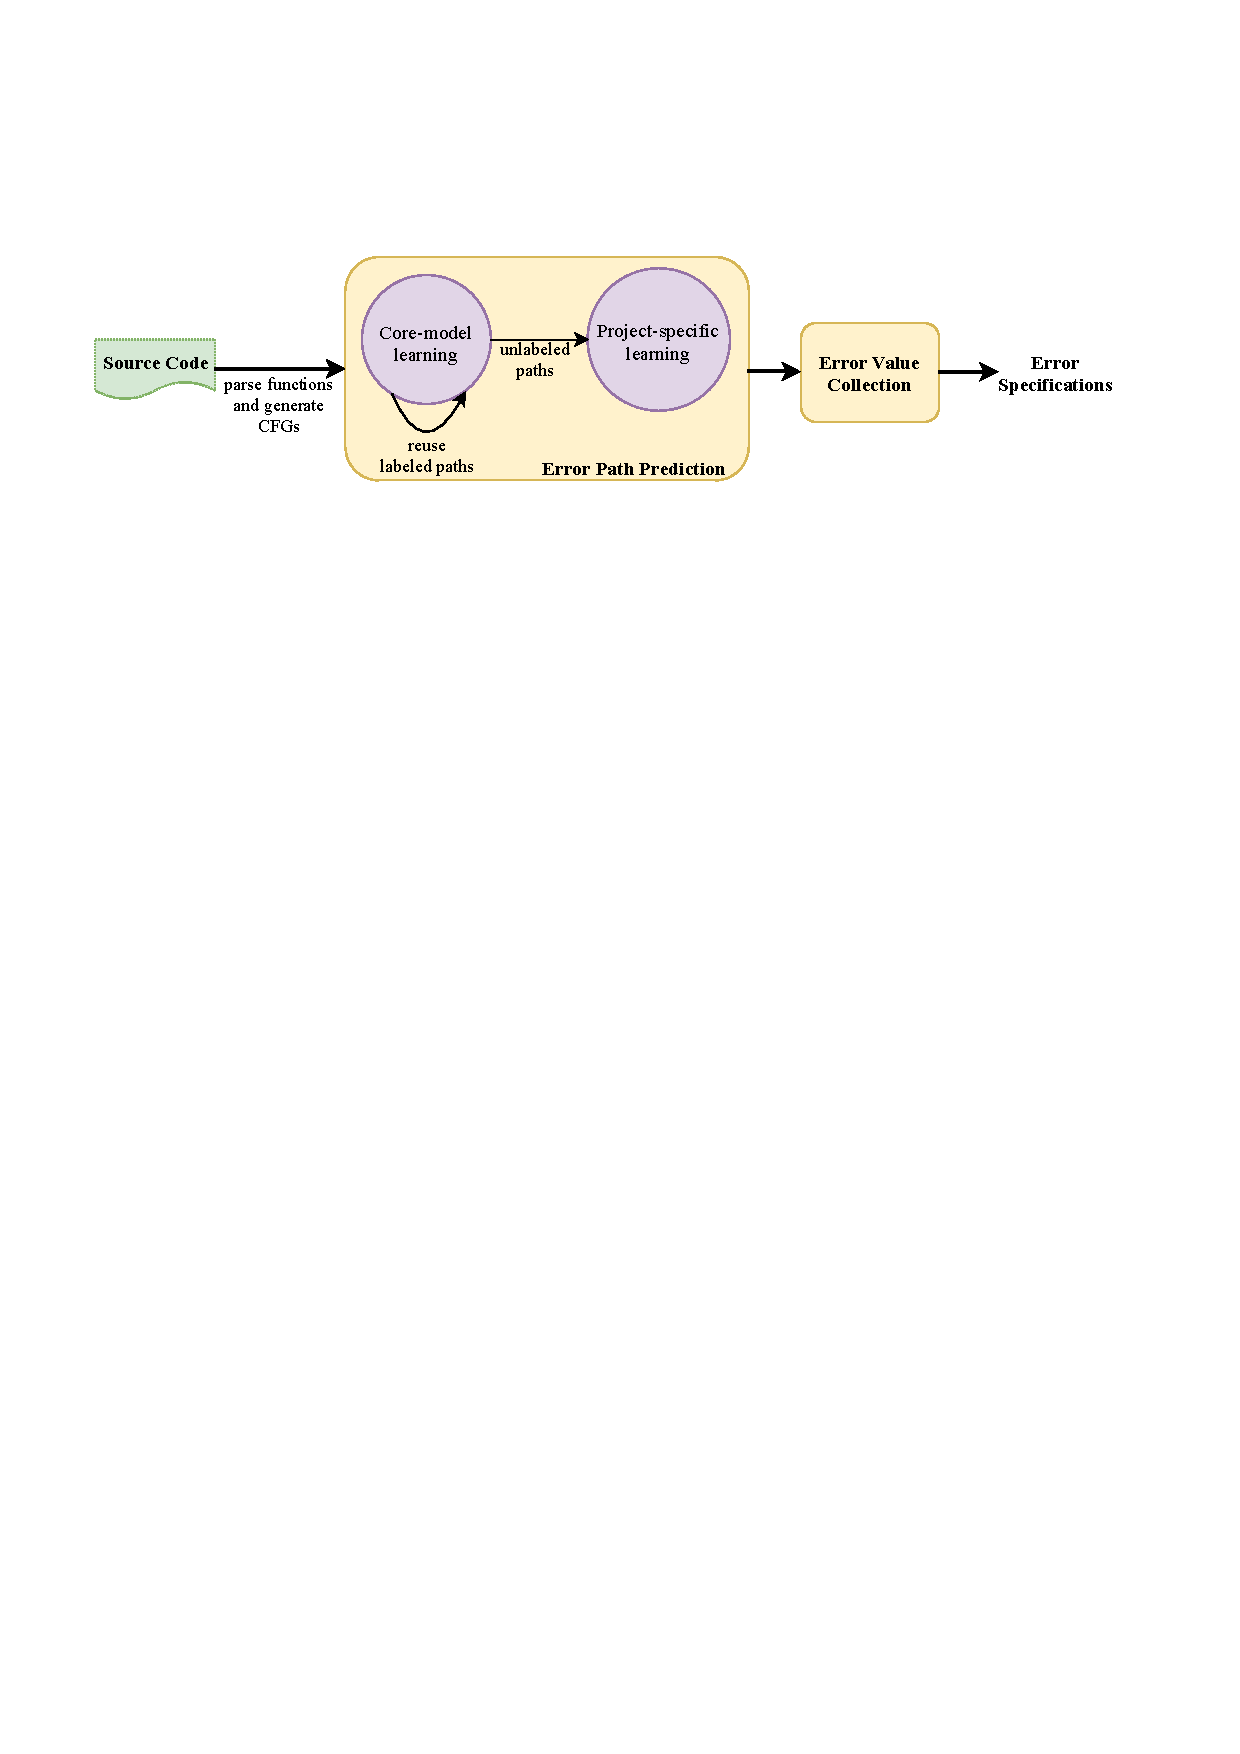
\includegraphics[width=0.95\linewidth]{images/errspec_arch.pdf}
\caption[The workflow of \newTool]{The workflow of \newTool.
Given a new project, 
\newTool\ first samples its most likely error and non-error paths in source code as the training data (Section~\ref{sec:app:learning:phase1}), 
from which a project-specific model is learned for classifying all paths in the new project (Section~\ref{sec:app:learning:phase2}). 
\newTool\ generates the error specification for a function by collecting return values of all its error paths (Section~\ref{sec:app:impl}). 
}
\label{fig:workflow}
\end{figure}

The rest of the chapter is organized as follows.
Section~\ref{sec:app:overview} shows the overview of \newTool.
Section~\ref{sec:app:features} discusses the features selected to characterize error paths.
Sections~\ref{sec:app:learning} presents the two learning phases for path classification.
%
%Section~\ref{sec:core-learn} and ~\ref{sec:project-learn} present the two learning phases for predicting error paths, respectively.
%Section~\ref{sec:fe} gives the features extracted in \newTool.
%Section~\ref{sec:spec-generate} provides the method of generating error specifications for each function.
%
Section~\ref{sec:app:impl} describes the implementation of \newTool.
Section~\ref{sec:app:eval} presents the evaluation results of our approach.
To illustrate the usefulness of error specifications, I present an
application of detecting error handling bugs in Section~\ref{sec:app:evalbugs}.


\section{Overview}
\label{sec:app:overview}

Before presenting our approach design, I first define paths, 
which, in turn, relies on the notion of Control Flow Graphs.
Both definitions are conventional in the literature.


\theoremstyle{definition}
\begin{definition}{\textbf{Control Flow Graph (CFG):}}
A CFG of a function in the program is a directed graph represented by a tuple $\langle N, E \rangle$. 
$N$ is the set of nodes, where each node is labeled with a unique program statement. 
The edges, $E \subseteq N \times N$, represent possible flow of execution between the nodes in the CFG. 
Each CFG has a single begin, $n_{\it{begin}}$, and end, $n_{\it{end}}$. 
All the nodes in the CFG are reachable from the $n_{\it{begin}}$ 
and the $n_{\it{end}}$ is reachable from all nodes in the CFG~\cite{Person:2011:DIS:1993498.1993558}.
\end{definition}

\begin{definition}{\textbf{Path:}}
A path is a sequence of nodes 
$\langle n_0, n_1, .... n_j \rangle$ in a CFG, 
such that there exists an edge $e_{k, k+1} \in E$ between $n_k$ and $n_{k+1}$, 
%i.e. $(n_k,n_{k+1}) \in E$, 
for $k = 0,...,j-1$~\cite{Nejmeh:1988:NME:42372.42379}.
\end{definition}

In this chapter, a path in a given function \prog{f()} starts from the entry $n_{\it{begin}}$ of \prog{f()}
and ends at the exit $n_{\it{end}}$ of \prog{f()}.
Language constructs,
such as \prog{for}, \prog{while}, and \prog{goto},
may introduce cycles in a CFG,
yielding an infinite number of paths.
To avoid this issue, we require that each single path does not contain duplicate nodes. 
%
Other work~\cite{Kang:2016:AAI:2970276.2970354,Tian:2017:ADR,jana2016automatically}
faced the same issue and used a similar solution. 

\subsection{Approach Design}
\label{sec:app:overview:design}

Since collecting error specifications is easy once we have identified
error paths, I focus on error path identification 
until Section~\ref{sec:app:impl}, where I discuss error specification collection.

Many recent approaches~\cite{wu2017learning,Eric2017learning,balog2016deepcoder,pradel2018deepbugs}
%~\cite{Wu2017learning,Eric2017learning,balog2016deepcoder,pradel2018deepbugs} 
have employed supervised learning to solve some programming language problems. 
%
To achieve a good learning performance, there are two basic paradigms:
learning a global model for different projects or learning a 
per-project model for individual projects. Each paradigm suffers
from some shortcomings. I propose a new paradigm that uses 
two-phase learning to avert the shortcomings with these basic
paradigms. 

\parag{Learning a global model.}
%
As shown in Figure~\ref{fig:mmodels:global},
a global model is trained from a large set of training data,
such that it can generalize to new data.
%
We may think of following this idea to develop a model for predicting whether 
a path is error or non-error. This involves the following steps. 
(1) We design a set of universal features that can characterize paths across projects. 
(2) We label each path as error or non-error from a considerable number of projects. 
(3) We train a model from the labeled paths to relate
feature values with labels by using some supervised machine learning method~\cite{hastie2009overview}.
After that, users could directly apply the trained model to new projects for predicting error paths.

The global model is essentially a data hungry model,
and its main drawback is that the size of data needed to train an accurate model is usually up to hundreds of mega bytes,
or even giga bytes~\cite{russakovsky2015imagenet}.
%For example, ImageNet~\cite{russakovsky2015imagenet} provides 456,567 labeled images as the training data for visual recognition. 
Obviously, in practice it is usually infeasible to obtain such a large amount of labeled data for training a global model. 
%
In the process of solution searching,
we trained a global model from 300 labeled paths 
and observed that its error path prediction accuracy is about 65\% only.

\begin{figure}[t]
\centering
\begin{subfigure}[b]{0.3\textwidth}
	\centering
    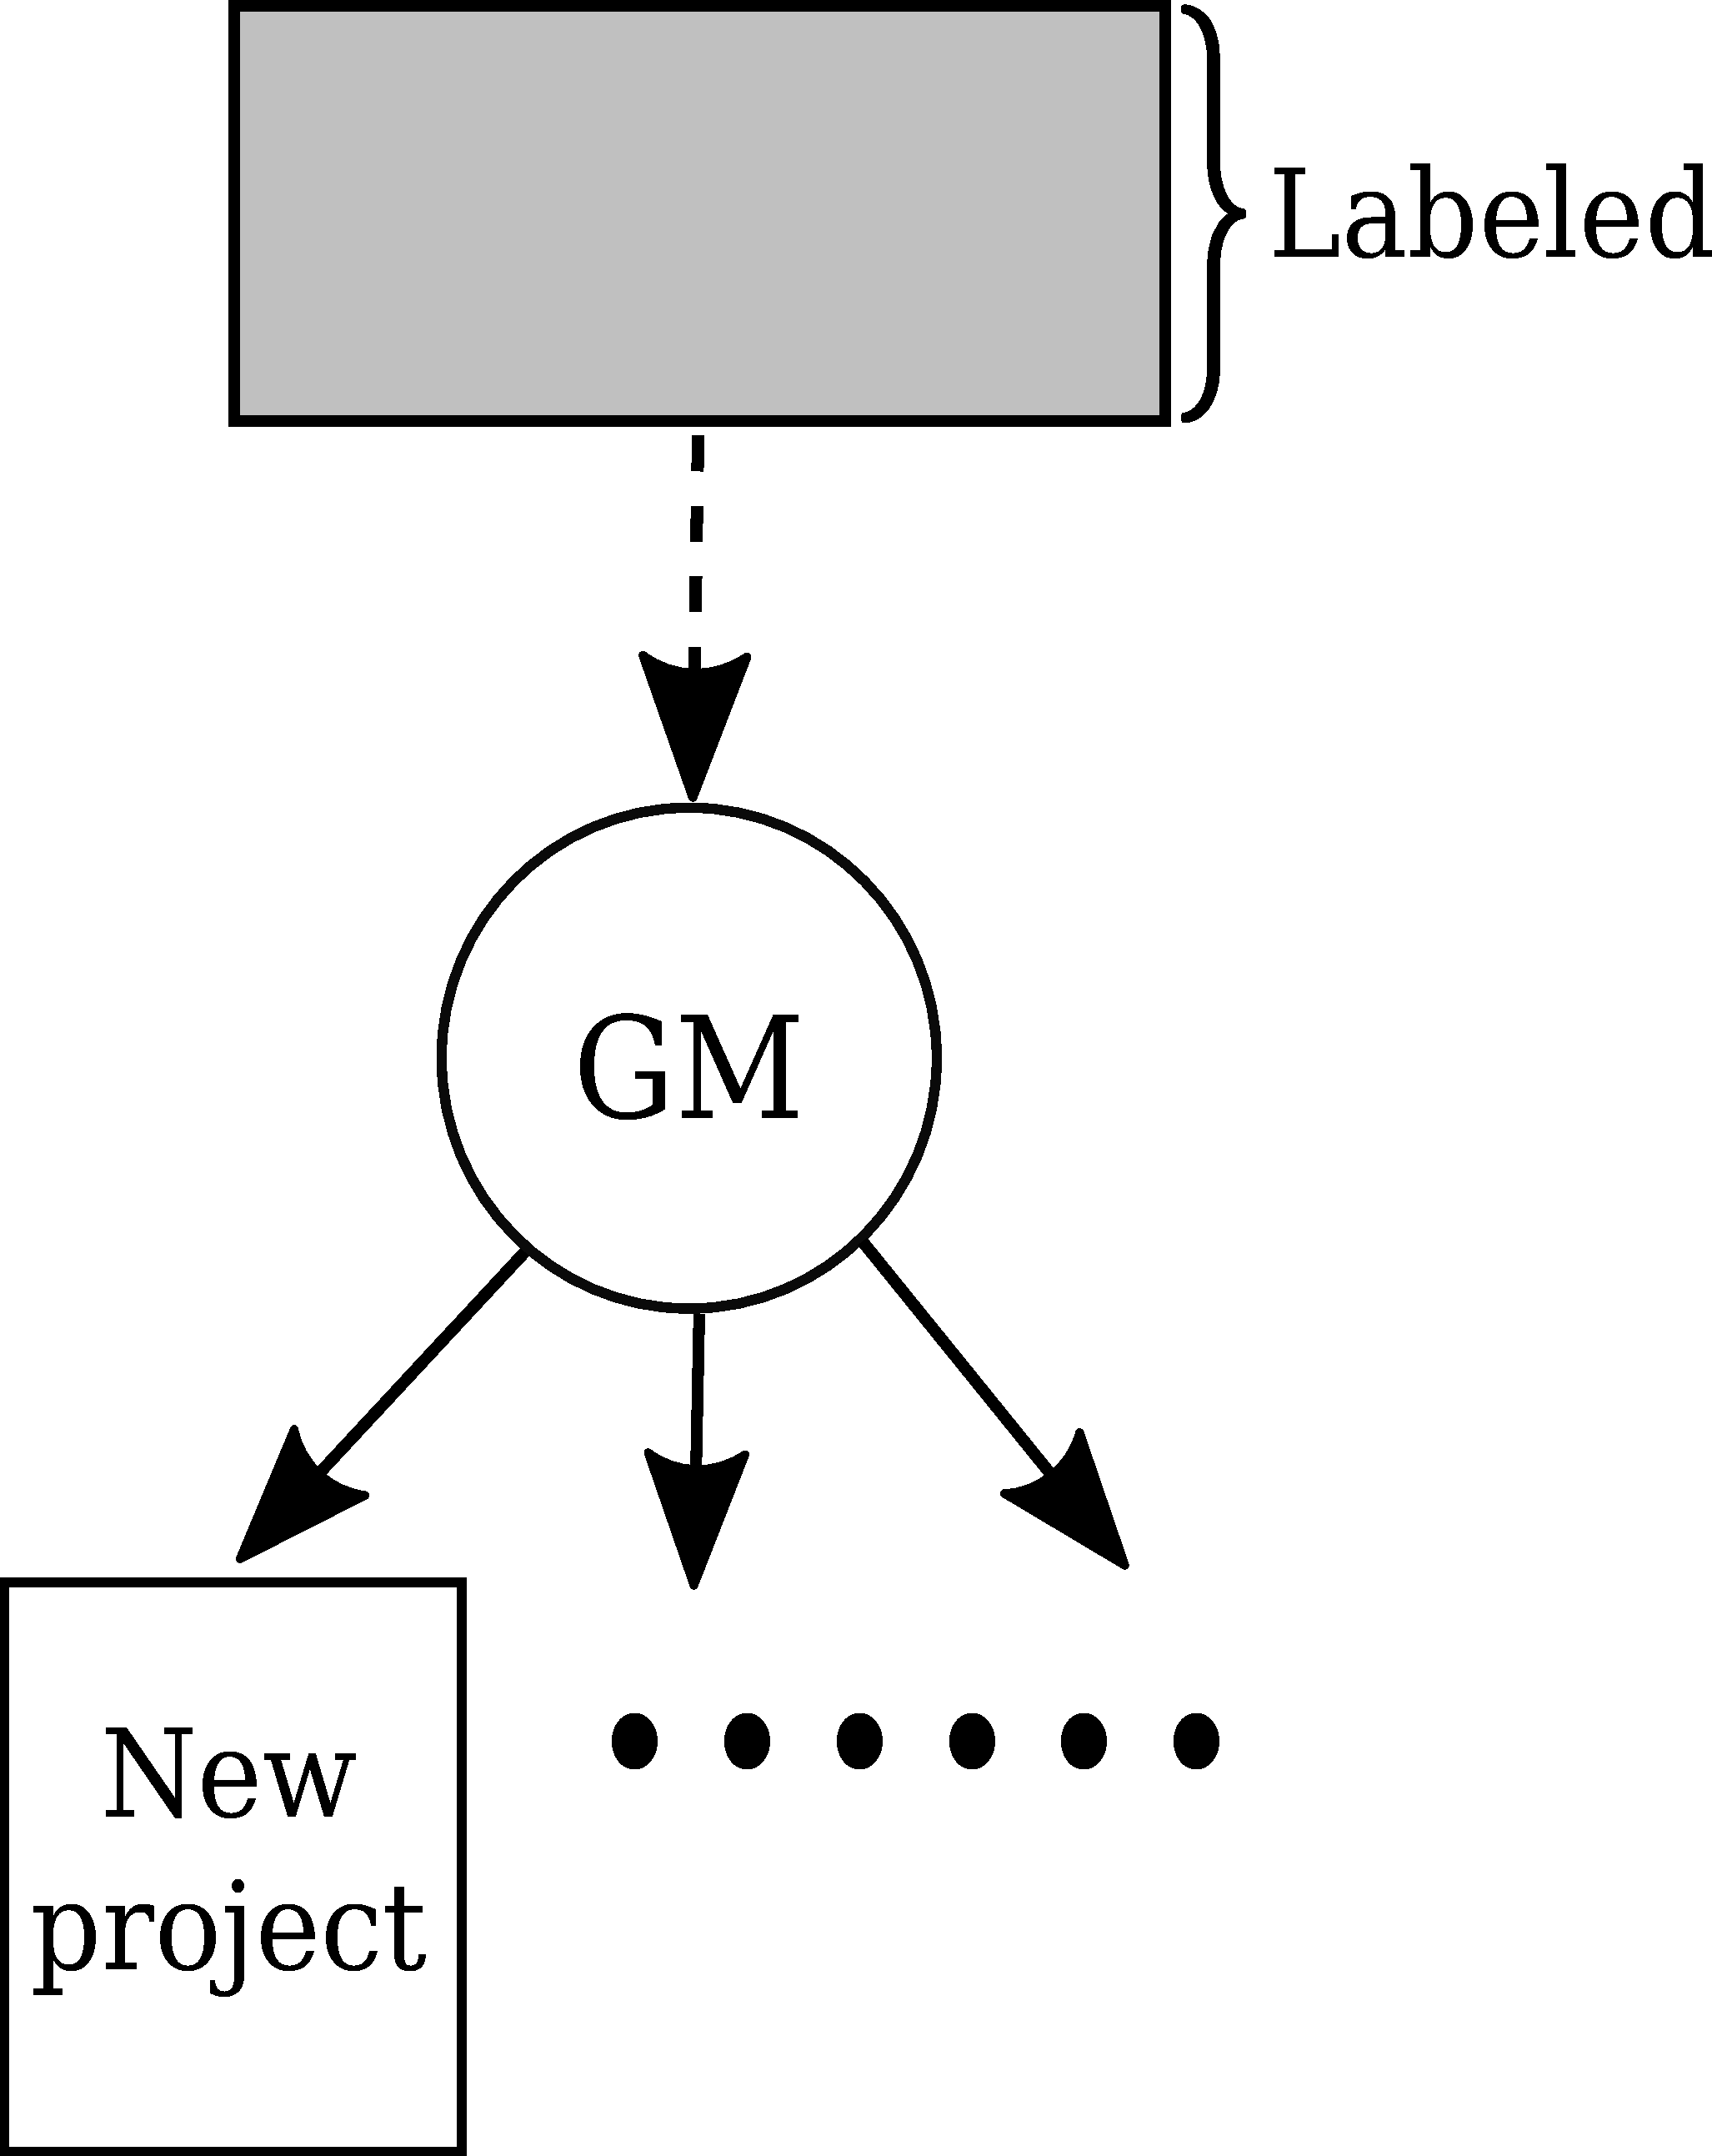
\includegraphics[width=.75\linewidth]{images/global-m.pdf}
    \caption{Global \paradigm}
     \label{fig:mmodels:global}
\end{subfigure}%
\hfill
\begin{subfigure}[b]{0.3\textwidth}
	\centering
    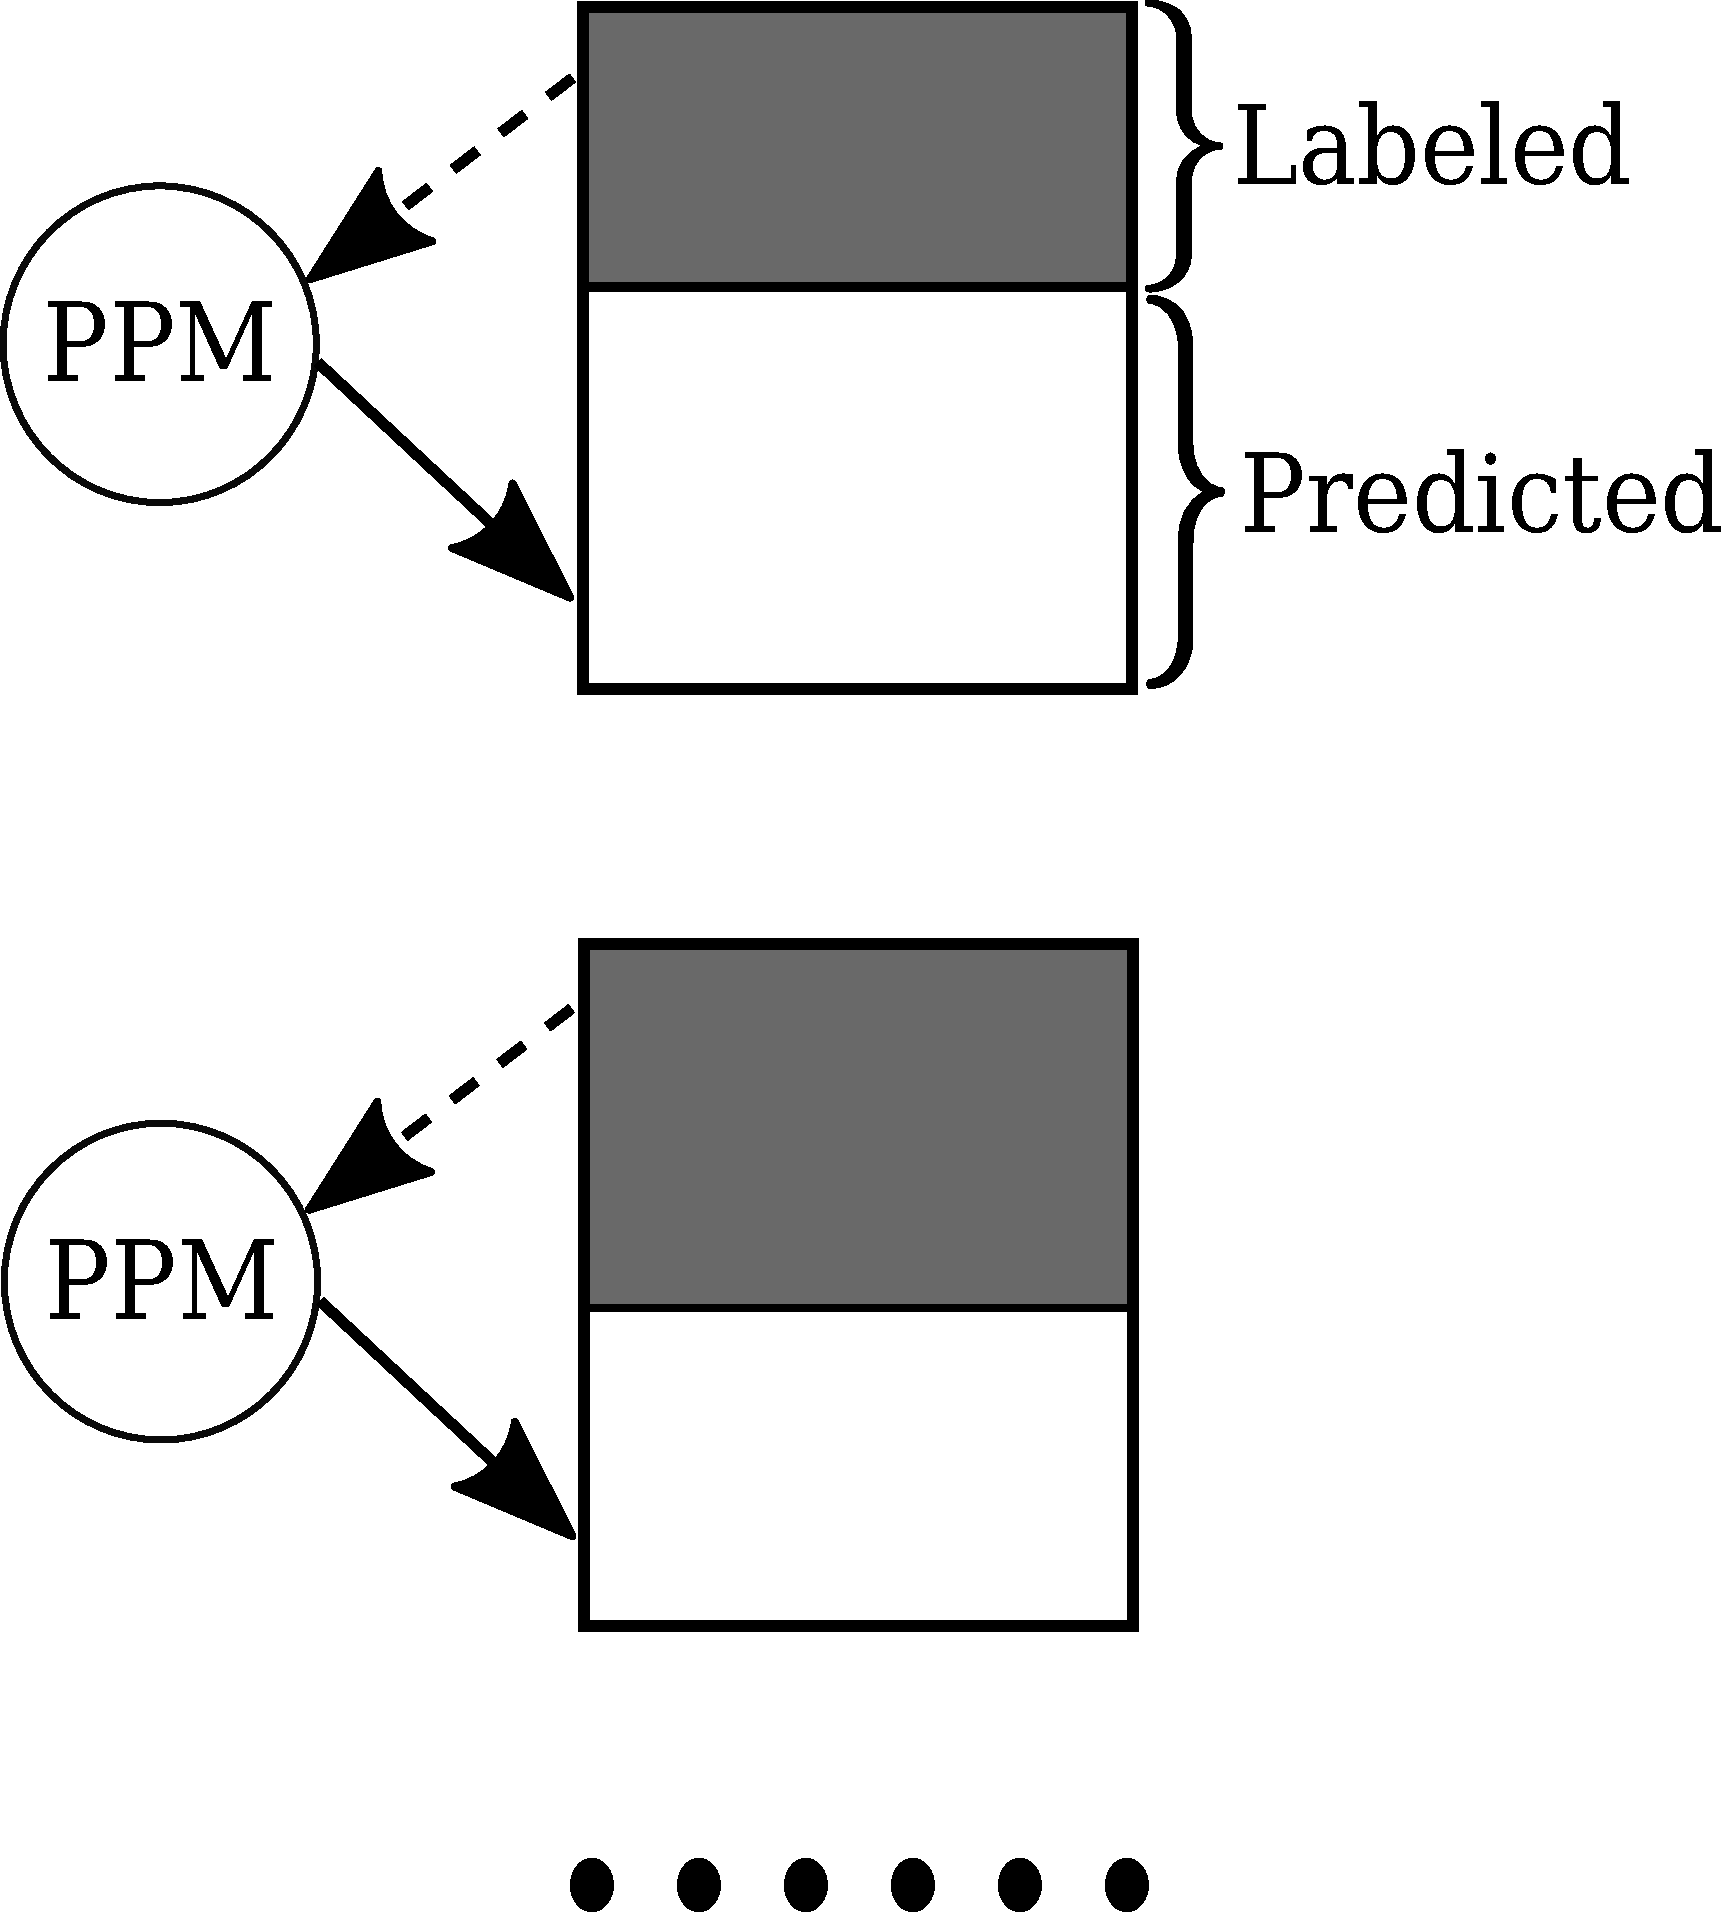
\includegraphics[width=.85\linewidth]{images/per-project.pdf}
    \caption{Per-project \paradigm}
    \label{fig:mmodels:pproject}
\end{subfigure}%
\hfill
\begin{subfigure}[b]{0.4\textwidth}
	\centering
    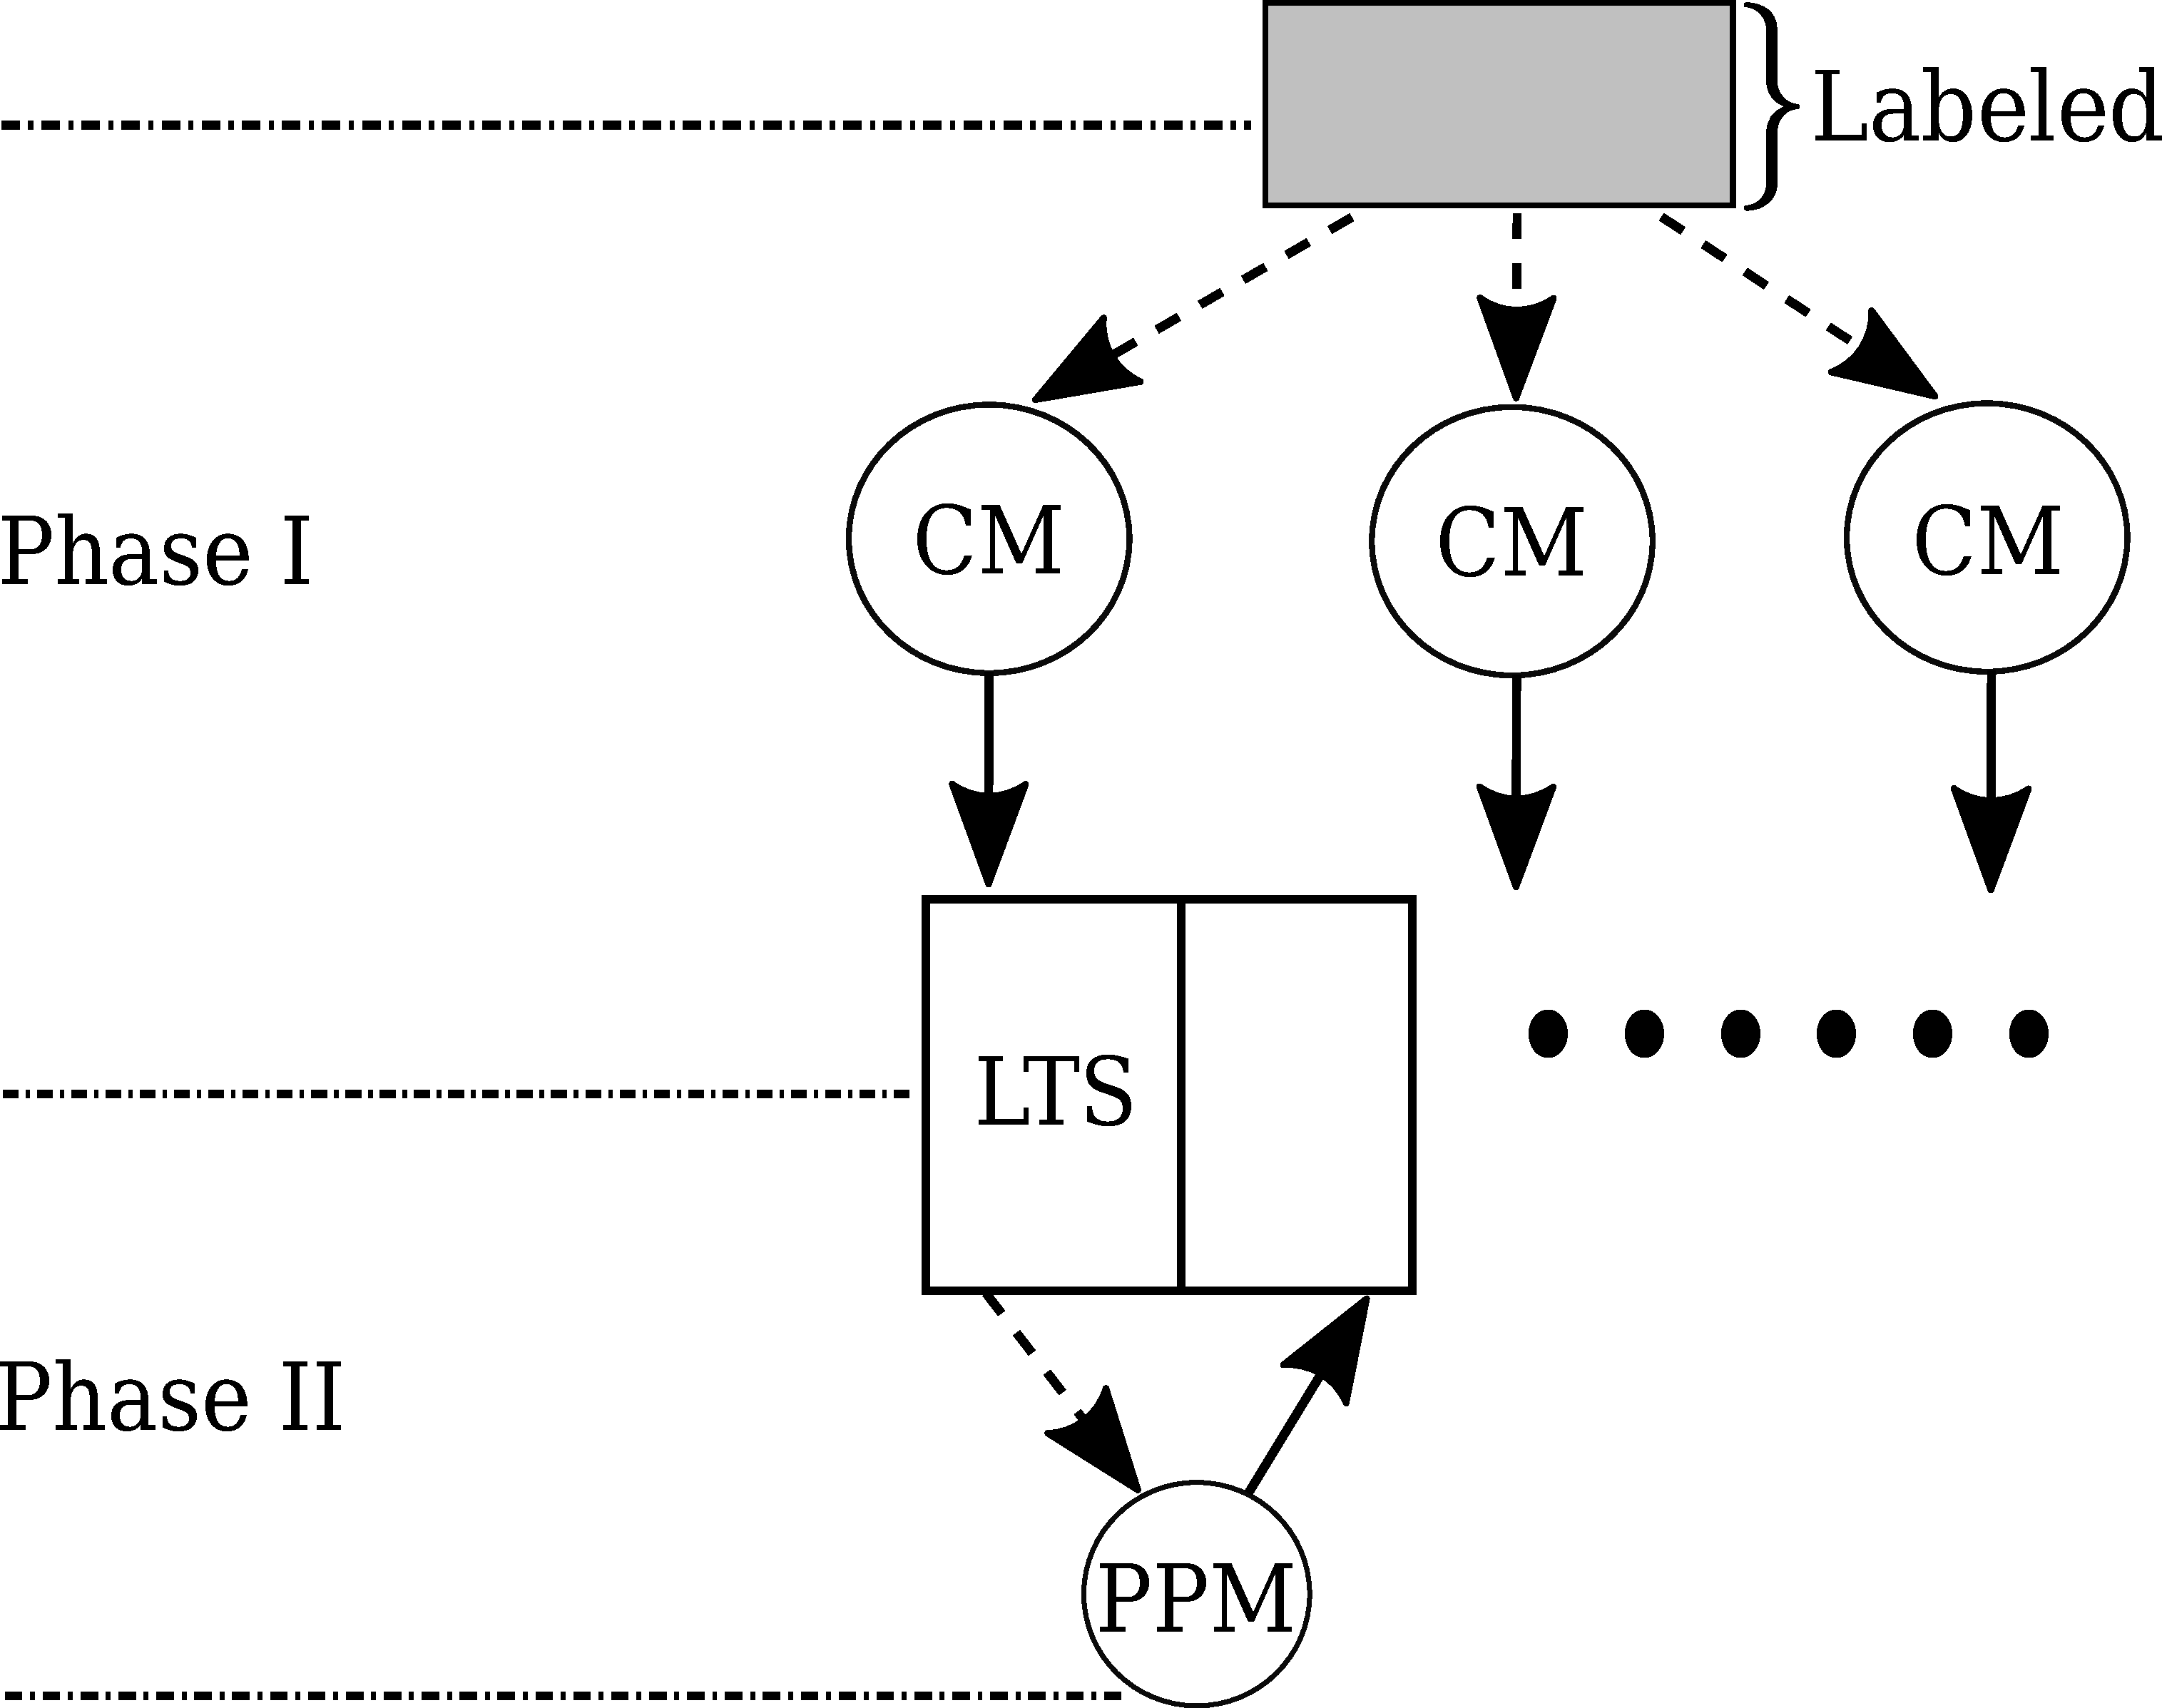
\includegraphics[width=.9\linewidth]{images/two-phase.pdf}
    \caption{Two-phase \paradigm}
    \label{fig:mmodels:tphase}
\end{subfigure}
\caption[Different learning \paradigm{s}]{Different learning \paradigm{s}. 
Obtaining the light-grey and dark-grey objects 
need manual labeling efforts from the researcher and the user, respectively.
Each dotted arrow denotes the direction of learning a model from labeled paths,
and each solid arrow indicates the direction of predicting the ``target'' with a model.
%Each big rectangle represents a new project. 
We use the acronyms ``GM'', ``PPM'', ``CM'' and ``LTS'' to represent
global model, per-project model, core model and learned training set, respectively.
}
\label{fig:mmodels}
\end{figure}

\begin{figure}[t]
\begin{Verbatim}[numbers=left,xleftmargin=6mm,fontsize=\footnotesize,
    commandchars=\\\{\}]
\it{/* vlc-2.1.4/src/posix/thread.c */}
int vlc_sem_post(vlc_sem_t *sem)
\{
  int val;
  if (likely(semaphore_signal(*sem) == KERN_SUCCESS))
    \correctline{return 0;}
  ...
  if (unlikely(val != EOVERFLOW))
    VLC_THREAD_ASSERT("unlocking semaphore");
  \errline{return EINVAL;}
\}
\end{Verbatim}
\caption[An example of error and non-error paths in VLC]{An example of error and non-error paths in VLC.
The path returning 0 (marked in bold-green) is a non-error path, 
while that returning \prog{EINVAL} (marked in italic-red) is an error path.
}
\label{fig:unifeature-exam}
\end{figure}

\parag{Learning a per-project model.}
%
One reason that the global model trained from a small set of labeled paths
does not perform well is underfitting~\cite{alpaydin2009introduction}.
%
For example, as shown in Figure~\ref{fig:unifeature-exam},
the error path in \prog{vlc\_sem\_post()} is longer than the non-error path,
contradicting the intuition that in C the lengths of error paths are usually smaller than those of non-error paths.
%
If the amount of training data is small,
such cases are not seen often enough by the global model
and thus cannot be handled well.
%due to the statistical issue of underfitting~\cite{alpaydin2009introduction}.
%
To address this, we can either provide more training data including sufficient ``corner'' cases, 
ending up in a global model,
or incorporate more features that bring extra information to learn a more representative model~\cite{hua2004optimal,zhang2018strategy},
leading to this second learning paradigm.
%

The main idea here is to leverage domain 
knowledge to extract project-specific features
and combine them with universal features to learn a per-project model,
as shown in Figure~\ref{fig:mmodels:pproject}.
Project-specific features are closely related to the learning task 
and are helpful to improve the prediction performance of the trained model~\cite{kopanas2002role}.
%
Take the function \prog{vlc\_sem\_post()} as an example. 
It is quite easy for human beings to 
classify the path returning 0 as a non-error path
and the one returning \prog{EINVAL} as an error path.
%
The reason is that the former path ends in the true branch of an if-statement
whose condition compares with \prog{KERN\_SUCCESS}, 
a value that usually indicates correct program executions.
Similarly, the latter path returns \prog{EINVAL},
a value usually returned
by functions to indicate the occurrence of errors.
%
As a result, using that if-statement and the return expression \prog{EINVAL}
as two project-specific features can help better identify error and non-error paths in project VLC.
For instance, if the return expression of a new path is \prog{EINVAL},
then the new path is likely to be an error path in VLC.

The shortcoming of a per-project model is that
the user needs to manually provide domain knowledge for training a model,
and the process has to be repeated for each project
because the domain knowledge is project-specific.
For example, zlib uses \prog{Z\_OK} to indicate non-error situations 
while VLC never uses such conventions. 


\parag{Two-phase learning paradigm.}
%
The \paradigms\ for training a global model (Figure~\ref{fig:mmodels:global}) 
and a per-project model (Figure~\ref{fig:mmodels:pproject}) have their respective advantages, 
and the advantage of one \paradigm\ is the disadvantage of the other. 
%
For example, the advantage of the global \paradigm\ is that the user does not have to 
label any paths and the disadvantage is that it requires a very large training data set
to generate a representative model.
%
%the error path prediction precision may be low due to the lack of domain knowledge. 
In contrast, the per-project \paradigm\ utilizes project-specific features extracted from domain knowledge
to train a model from a relatively small training data set,
but it requires users to provide the domain knowledge for each new project,
which is tedious and hinders its applicability.

Surprisingly, we can integrate the global \paradigm\ and per-project \paradigm\
cogently with the following key observations. 
%
\begin{enumerate*}[label={(\arabic*)}]
%
\item Give a small training data set, 
while the global model fails to accurately classify all paths in a new project,
it can do so for a certain portion of paths.
%since the knowledge learned by the global model could be transferred 
%to the new project through universal features~\cite{pan2010survey}.
We refer to that portion of paths as the learned \typical\ set (LTS).
LTS contains both error and non-error paths and should be
highly accurate. 


\item Project-specific domain knowledge can be 
obtained by extracting relevant information from LTS.
For example, if a path in LTS returning \prog{EINVAL} is labeled as an error path,
then it is sensible to infer that \prog{EINVAL} represents error paths in the project.

\end{enumerate*}

This integration leads to the two-phase \paradigm\ shown in Figure~\ref{fig:mmodels:tphase}. 
In phase I, we first learn a core model for each new project 
based on the knowledge transferred from a set of per-labeled paths.
Then, we construct LTS by getting the paths for which the core model is highly confident in its classification.
%
In phase II, we learn a per-project model from LTS
and use it to identify error paths in the corresponding new project.
The proposed two-phase \paradigm\ provides a nice property:
it requires one-time minimal labeling efforts from us
to initialize \newTool\
and zero manual work from users
to predict error paths in different projects.
%
In this chapter, we use this paradigm to classify paths into error
or non-error. We formalize this paradigm in Section~\ref{sec:app:learning}.



\section{Path Features}
\label{sec:app:features}

This section presents the features used to classify the paths in C programs.
The features are directly extracted from source code and are related to program behaviors.
A path can be represented by a path feature vector that stores the feature values.
I give an overview of the features and their values in Figure~\ref{tab:features}.
I discuss universal features in Section~\ref{sec:app:features:uni}
and project-specific features in Section~\ref{sec:app:features:pp}.
Statistical analysis is preformed to validate the used features in Section~\ref{sec:app:features:valid}.

\begin{figure}[t]
\centering
\begin{tabular}{c | l l }
\toprule
%ID &  Message information contained in the category \\
ID & Summary & Feature Values  \\
\midrule
1 & Path length & Float (0.0 $\sim$ 1.0]\\
2 & \# of expression statements & Float [0.0 $\sim$ 1.0] \\
3 & \# of function calls & Float [0.0 $\sim$ 1.0] \\
4 & \# of if-conditions & Float [0.0 $\sim$ 1.0] \\
5 & Spanning distance of return expression & Float (0.0 $\sim$ 1.0] \\
6 & Kind of return expression & Nominal [0 $\sim$ 4] \\
7 & Kind of return value & Nominal [0 $\sim$ 3] \\
\midrule
8 & Presence of the return expression in set \errsetRetVar\  & Nominal [0 $\sim$ 1]\\
9 & Presence of the return expression in set \nerrsetRetVar & Nominal [0 $\sim$ 1]\\
10 & Presence of the if-conditions in set \errsetLastCond\ & Nominal [0 $\sim$ 1]\\
11 & Presence of the if-conditions in set \nerrsetLastCond & Nominal [0 $\sim$ 1]\\
12 & Presence of the called functions in set \errsetLastFunc\  & Nominal [0 $\sim$ 1]\\
13 & Presence of the called functions in set \nerrsetLastFunc & Nominal [0 $\sim$ 1]\\ 
\bottomrule
\end{tabular}
\caption[An overview of path features]{An overview of path features. 
The first seven features are universal features,
and the rest are project-specific features.
%We use the short name expr for expression.
We normalize the values of the first five features.
A ``Nominal'' feature takes any integral value specified in the corresponding range.
}
\label{tab:features}
\end{figure}

\subsection{Universal Features}
\label{sec:app:features:uni}

Usually, a function in C checks against different errors before returning the final result of normal execution,
and it returns the corresponding error immediately when failing on any such check.
To capture this characteristic,
we consider the distance between the entry point and the corresponding exit point (feature 1),
the number of expression statements (feature 2), the number of function calls (feature 3), the number of if-conditions (feature 4),
and the spanning distance with respect to lines of code from the entry point to the corresponding exit point (feature 5).

We normalize the values of the first five features to make them meaningful across different functions and projects.
Specifically, for each feature, we divide every non-normalized value
by the largest non-normalized value of all paths from the same function.
For example, if a path has length 3 and the longest path in the corresponding function is 10,
then the normalized value of feature 1 for that path is 0.3.

Moreover, C functions return different kinds of expressions, such as macro and constant,
and different kinds of values, such as positive and negative values,
to represent the execution results in error or non-error situations.
%
The return expression kind and return value kind could thus indicate if a path is error or non-error.
For example, functions tend to use macros with negative values as error returns in C projects.
We use feature 6 and 7 to describe the two return kinds.

To compute the values for features 6 and 7, we first 
perform aggressive substitutions to make the result more accurate. 
%
Specifically, we substitute variables with expressions based on the corresponding data flows.
For example, in Figure~\ref{fig:errhandlingbug}, 
the return variable \prog{tlv} in line 19 is substituted with \prog{kzalloc(...)}.
%
Based on the substituted return expression, for feature 6, 
we assign 0 if it is a macro,
%(if all characters in the identifier are all upper case or the identifier is \prog{true} or \prog{false}), 
1 if it is a constant, 
2 if it is a function call,
%(such as \prog{f(...)} where \prog{f} is a function), 
3 if it is an expression 
(such as \prog{a+b} where \prog{a} and \prog{b} are two expressions), 
and 4 if it is a variable.
%(such as a parameter to the enclosing function).
%
For example, if two paths share the same return statement \prog{return ret}
but the first path has the assignment \prog{ret=false} before return 
and the other has \prog{ret=f(...)}, then the values for feature 6 
are 0 and 2 for the two paths, respectively. 
%

For feature 7, we assign 0, 1, and 2 if the substituted return expression can be evaluated 
to 0, a positive value, and a negative value,
respectively, and 3 if the value cannot
be statically known. 
%
We do not directly encode the return expressions and return values as features.
The reason is that, by doing this, the features would have too many possible values, which will hurt 
machine learning performance according to the bias-variance tradeoff~\cite{geman1992neural}.

\subsection{Project-specific Features}
\label{sec:app:features:pp}

Using project-specific features can better characterize paths
since they provide more relevant information about path erroneousness/non-erroneousness.
In each path, project-specific information usually appears in 
three places. The first is the return expression. 
%It's a quite common idiom to define error code as macros and then return
%them in error paths. 
Error paths within the same project use a set of predefined idioms to represent error code.
%
%Error codes are often defined as macros in C and returned in error paths.
For example, the functions in httpd
return the macros \prog{AP\_NOBODY\_READ} and \prog{AP\_FILTER\_ERROR} to indicate errors. 
We use \errsetRetVar\ and \nerrsetRetVar\ to represent the sets of error and non-error
return expressions in a project, respectively.


The second place is the latest if-condition before the
path returns since programs usually test with certain conditions
to decide whether the current status is still normal or not. For example,
in httpd, several functions perform the following test
\prog{(VAR\_NAME->VAR\_NAME)==HTTP\_BAD\_GATEWAY}
(\prog{VAR\_NAME} represents any variable name)
to indicate that a server received an invalid response and 
take corresponding actions. 
We use \errsetLastCond\ and \nerrsetLastCond\ to represent the sets of the latest if-conditions
that appear in error and non-error paths, respectively.


The third place is the functions called within the latest conditional
before the return statement. 
The rationale is that functions 
usually perform similar clean-ups (e.g. release a lock or free some dynamically 
allocated memory) or loggings before returning from error/non-error paths. 
This is particularly true for error paths.
For example, in httpd, functions
%\prog{AP\_READ\_REQUEST\_FAILURE}, 
\prog{ap\_log\_rerror} and
\prog{ap\_abort\_on\_oom} are used when related errors occur. 
We use \errsetLastFunc\ and \nerrsetLastFunc\ to represent the sets of such functions
in error and non-error paths, respectively.

The six sets could be distilled from training data, i.e., a set of labeled paths.
%
From the labeled error paths,
extracting \errsetRetVar\ and \errsetLastFunc\ is straightforward but extracting
\errsetLastCond\ has some subtlety. In particular, conditions may involve
variables, such as \prog{rv == AP\_FILTER\_ERROR}. Recording the whole 
condition in the set maybe not very helpful since other places could
use different variables to compare with \prog{AP\_FILTER\_ERROR}. We address
this issue by replacing all variables in conditions with \prog{VAR\_NAME}. 
%
For example, if the training data contains the two error paths in Figure~\ref{fig:errspec},
then we add ``\prog{Z\_STREAM\_ERROR}'' and ``\prog{Z\_BUF\_ERROR}'' to \errsetRetVar,
and add ``\prog{deflateStateCheck(VAR\_NAME)} == True'' 
and ``\prog{VAR\_NAME < ...} == True'' to \errsetLastCond.
%
Similarly, we extract \nerrsetRetVar, \nerrsetLastCond, and \nerrsetLastFunc\ from the labeled non-error paths. 

It is possible that \errsetRetVar\ and \nerrsetRetVar\ are overlapping, 
which means that either there exist incorrectly labeled paths in the training data,
or some return expressions appear in both labeled error and
non-error paths, for example \prog{0} can be used to indicate both error and non-error in Linux kernel.
%
Such return expressions are not associated with error or non-error situations. 
We thus remove the overlapping elements from both \errsetRetVar\ and \nerrsetRetVar. 
Similarly, we do this for \errsetLastCond\ and \nerrsetLastCond\ and for \errsetLastFunc\ and \nerrsetLastFunc\ when overlapping happens.

The project-specific features are then extracted in terms of the presences of the six sets in each path.
%
%Given the six sets of project-specific information, 
%we extract six project-specific features based on their presence in each path.
Specifically, for feature 8, we assign 1 if the return expression of the path appears in \errsetRetVar,
and 0 otherwise. We compute the values for the other project-specific features in the same way.

\subsection{Feature Validation}
\label{sec:app:features:valid}

We perform Chi-square analysis~\cite{liu1995chi2} to investigate the usefulness of path features,
which is a standard method of feature validation~\cite{li2018feature}.
%
Specifically, we randomly selected 300 functions from libc, Linux and httpd, 
which are different from the evaluated functions in Section~\ref{sec:app:eval}.
%functions that we evaluate in Section~\ref{sec:eval}.
We manually labeled all 1604 paths generated from these functions.
%
For each project, 100 randomly selected paths were used to extract the project-specific information
(i.e., the six sets such as \errsetLastFunc\ and \nerrsetLastFunc),
based on which we extracted project-specific features. 
%
%For each project, the project-specific features were extracted based on 100 randomly selected labeled paths.
%
The results of Chi-square analysis are presented in Figure~\ref{fig:chi2},
which contains two parts: $p$-value and $\mathcal{X}^2$ score.
The smaller the $p$-value,
the higher the significance that the feature is associated with path label.
In addition,
The higher the $\mathcal{X}^2$ score is, 
the more important the feature is for path classification~\cite{li2018feature}.
%
Based on the results,
we aim to answer the following two questions:

\par\smallskip
\noindent
\textit{Q1. Are all features relevant to the path classification?}
\smallskip

From Figure~\ref{fig:chi2},
we find that, for libc,
%
the $p$-values of all features are smaller than 0.05,
showing high-level significance when associated with path label.
We observe similar results for httpd and Linux.
%
Thus, the features used in our work are statistically correlated with error/non-error paths.

\begin{figure}
\centering
\begin{tabularx}{\textwidth}{ c c | Y | Y | Y | Y | Y | Y }
\toprule
\multicolumn{1}{c}{} 
 & \multicolumn{1}{c|}{} 
 & \multicolumn{3}{c|}{$p$-value}
 & \multicolumn{3}{c}{$\mathcal{X}^2$ score} \\
 & ID & libc & httpd & Linux & libc & httpd & Linux \\
\midrule
\multirow{7}{*}{\makecell{Universal\\features}}
& 1 & 2.1e-4 & 1.4e-4 & 4.6e-2 & 13.8 & 14.4 & 3.2 \\
& 2 & 2.3e-3 & 2.4e-3 & 3.1e-2 & 9.3 & 9.2 & 4.7 \\
& 3 & 2.1e-9 & 2.8e-7 & 2.8e-3 & 35.9 & 26.3 & 8.9 \\
& 4 & 1.4e-7 & 4.2e-4 & 6.2e-4 & 27.7 & 12.5 & 11.7 \\
& 5 & 7.9e-6 & 1.6e-5 & 3.1e-2 & 20.0 & 18.6 & 4.7 \\
& 6 & 4.4e-5 & 2.7e-5 & 9.5e-4 &  14.7 & 15.0 & 5.2 \\
& 7 & 1.4e-7 & 4.0e-6 & 8.7e-5 & 27.6 & 36.6 & 15.8 \\
\midrule
\multirow{6}{*}{\makecell{Project-specific\\features}} 
& 8 & 2.7e-16 & 5.8e-25 & 1.1e-18 & 67.0 & 106.4 & 77.85 \\
& 9 & 3.2e-11 & 4.0e-14 & 5.0e-6 & 34.5 & 57.2 & 20.8 \\
& 10 & 6.7e-7 & 2.2e-17 & 2.5e-5 & 24.7 & 71.9 & 17.7 \\
& 11 & 8.2e-32 & 7.1e-33 & 2.0e-15 & 137.8 &  142.6 & 63.1 \\
& 12 & 8.7e-85 & 2.5e-109 & 5.7e-79 & 380.7 &  493.5 & 354.3 \\
& 13 & 7.8e-56 & 1.4e-66 & 1.5e-49 & 247.8 &  297.1 & 219.0 \\
\bottomrule
\end{tabularx}
\caption[Results of Chi-square analysis on path features]{Results of Chi-square analysis.
For all three projects, the $p$-value of each feature is smaller than 0.05.
Moreover, the $\mathcal{X}^2$ scores of project-specific features
are in general higher than those of universal features.
}
\label{fig:chi2}
\end{figure}

\par\smallskip
\noindent
\textit{Q2. Can project-specific features help distinguish error paths from non-error paths?}
\smallskip

From Figure~\ref{fig:chi2}, we also find that the $\mathcal{X}^2$ scores of project-specific features
are higher than those of universal features across all projects.
For example, the average scores of universal and project-specific features in httpd are 18.9 and 194.8, respectively.
%
Therefore, considering project-specific features can effectively enhance 
the performance of error path prediction in machine learning.
To illustrate this, we visualize the spatial distribution of paths in httpd (using t-SNE~\cite{maaten2008visualizing}),
and then compare the path distributions with and without project-specific features in Figure~\ref{fig:distri2}.
It is clear to see that error and non-error paths become much more separable after considering project-specific features.
We make the same observations on libc and Linux.
%and present the comparison results in Appendix~\ref{sec:appa}.
The results suggest that a better path classifier could be learned from the feature space 
containing both universal and project-specific features.

\begin{figure}
\centering
\begin{subfigure}[b]{0.5\textwidth}
	\centering
    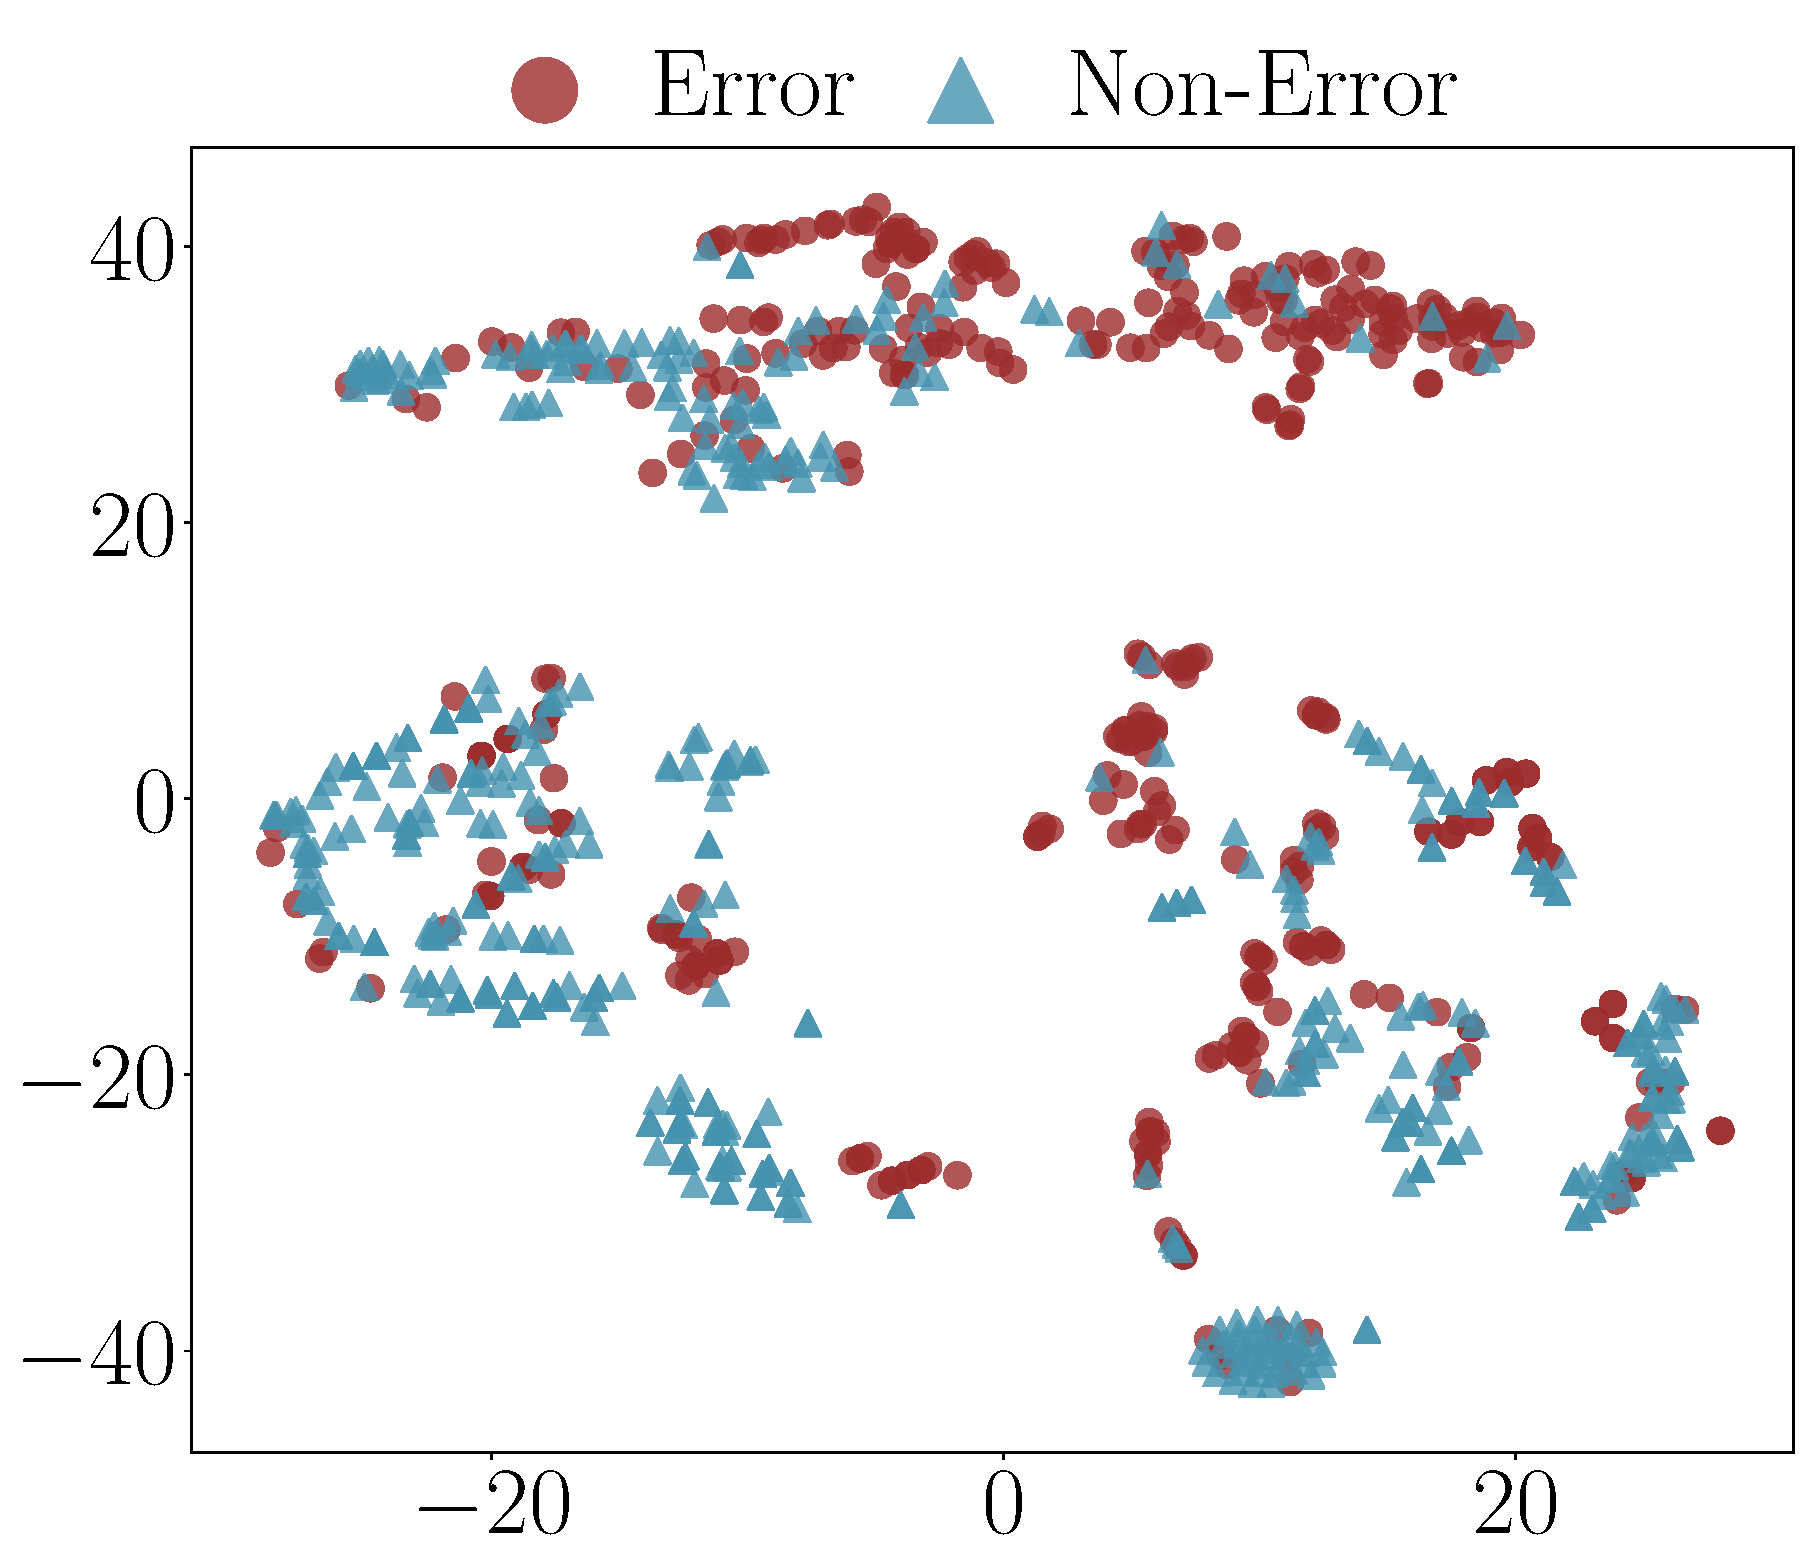
\includegraphics[width=.85\linewidth]{images/httpd_uni_feats.pdf}
    \caption{With only universal features.}
     \label{fig:distri2:uni}
\end{subfigure}%
\hfill
\begin{subfigure}[b]{0.5\textwidth}
	\centering
    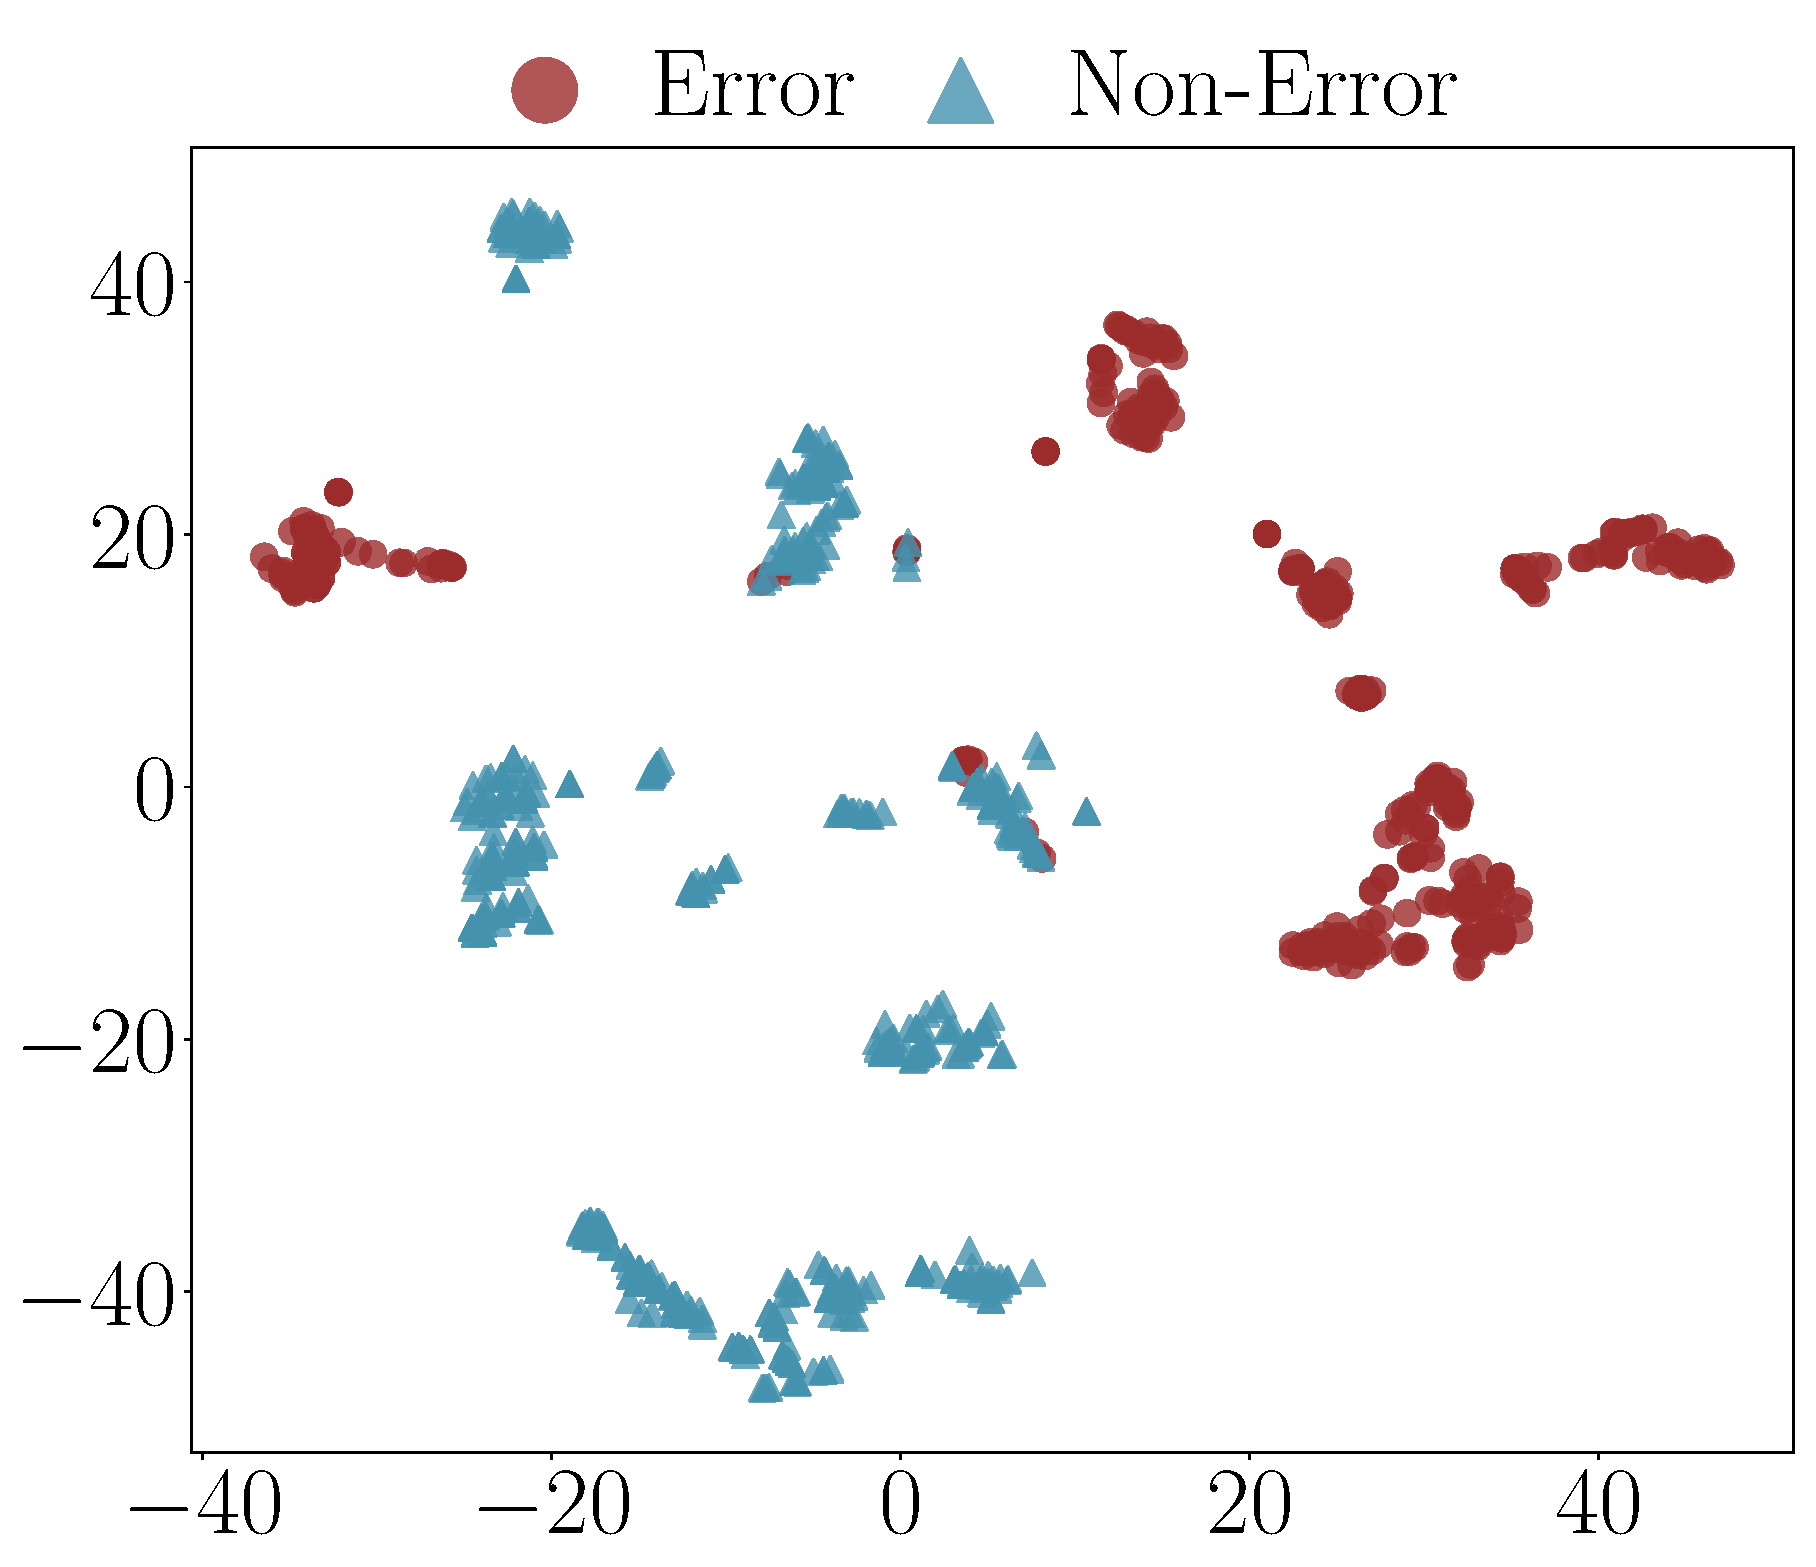
\includegraphics[width=.85\linewidth]{images/httpd_all_feats.pdf}
    \caption{With universal and project-specific features.}
    \label{fig:distri2:all}
\end{subfigure}
\caption[t-SNE visualization of path distributions in httpd]{t-SNE visualization of path distributions in httpd with and without project-specific features.
The error and non-error paths are easily separated after considering project-specific features.}
\label{fig:distri2}
\end{figure}

\section{Two-Phase Learning}
\label{sec:app:learning}

In general, the goal of supervised learning is to learn a model from a given
set of labeled instances (training set) and then use the learned model 
to make predictions for new instances. 
%
As discussed in Section~\ref{sec:app:overview:design},
there are two issues when applying traditional learning methods
on path prediction.
First, to make sure that the learned model generalizes well to new projects,
onerous manual efforts are required to label a large size of paths
such that the training set is representative enough.
Second, comparing to universal features,
project-specific features can improve the prediction accuracy.
However, the extracted project-specific features vary across projects
and thus can not be used as universal features,
i.e., we can not directly apply the project-specific features of one project to another.
The dilemma between choosing universal and project-specific features
limits the applicability of machine learning. 
%
To address these issues,
we proposed a novel two-phase learning paradigm in Section~\ref{sec:app:overview:design}.

The workflow of two-phase learning is as follows.
In \phasef, we learn a core model with universal features and
use it to automatically generate a learned training set for a new project.
In \phases, we extract project-specific features using the learned training set from \phasef, 
learn a per-project model, and apply it to the new project
to perform path predictions.
%
Each learning phase itself is a complete
learning process, and each phase consists of two steps: 
training and predicting. 
%The structures of 
%Sections~\ref{sec:core-learn} and~\ref{sec:project-learn}
%that present the two learning phases reflect this fact, 
%after we present the preliminaries of machine learning 
%in Section~\ref{sec:Preliminaries}.
%
To improve the readability of this section, we summarize 
the notations used in this section in 
Figure~\ref{tab:notation}.

\begin{figure}[t]
\centering
\begin{tabular}{r | l}
\toprule
Notations & \multicolumn{1}{c}{Interpretations}  \\
\midrule
$\Rset{d}$ & Real coordinate space of $d$ dimensions \\
$x$ & The feature vector of a path \\
$y$ & The label of a path \\
$(x, y)$ & A path whose feature vector is $x$ and label is $y$ \\
$\prb(y | x, \theta)$ & The probability that the label of a path is $y$ when the feature vector is $x$, \\
			& and $\theta$ is the parameter of the probability function \prb. \\ 
$\vec{X}$ & A set of path feature vectors \\
$\vec{Y}$ & A set of path labels \\
$\DS$ & The set of paths in the pre-labeled project \\
$\DT$ & The set of paths in the unlabeled project \\
$\ps(\vec{X}, \vec{Y})$ & The distribution of the paths in $\DS$ \\
$\pt(\vec{X}, \vec{Y})$ & The distribution of the paths in $\DT$ \\
$\DO$ & The learned training set \\
\sm\ & The model learned from \DS\ \\
\cm\ & The model learned from \DS\ and \DT \\
\ppm\ & The model learned from $\DO$ \\ 
$\gamma$ & The prediction confidence threshold \\
\bottomrule
\end{tabular}
\caption{Summary of the notations used in Section~\ref{sec:app:learning}.
}
\label{tab:notation}
\end{figure}

\subsection{Background of Supervised Learning}
\label{sec:app:learning:background}

As mentioned earlier, a supervised learning process consists of
both training and predicting. The goal of the training step
is to learn a probability description that can best 
approximate the distribution of the given training dataset. 
Concretely, let $(\vec{X}, \vec{Y}) = \{ (x_1,y_1),(x_2,y_2),\ldots,(x_n,y_n) \}$
denote a set of labeled paths $\D$,
where $x_i \in \Rset{d}$ is a vector containing $d$ features as the representation of path $i$,
and the class label $y_i \in \{ -1, +1\}$
indicates if path $i$ is error or non-error, respectively.
%
To learn the probability distribution of $\D$,
a common way is to use Maximum Likelihood Estimation (MLE)~\cite{vapnik2013nature}, expressed as follows:
%
\begin{equation} \label{mlsrc}
\theta^* 
 = \argmax_{\theta} \mathbb{E}_{(x, y) \in \D}[\ln \mathcal{L}(x, y, \theta)], 
%= \argmax_{\theta} \frac{1}{n} \sum_{i=1}^{n} \ln \mathcal{L}(x, y, \theta),
\end{equation}
%
where $\mathcal{L}(x, y, \theta)$ is the likelihood function in MLE that 
depends on its parameter $\theta \in \Rset{d}$.
%of $\mathcal{L}$.
In machine learning, the conventional choice of a likelihood function
could be an entropy function~\cite{nigam1999using}, 
the gini index~\cite{breiman2017classification},
or some form of regression function. 
%
Equation (\ref{mlsrc}) aims to find an assignment to the parameter 
$\theta$ that maximizes (expressed by $\argmax$)
the expected likelihood of the paths in $\D$ (expressed by $\mathbb{E}$). 
The best assignment to
$\theta$ is denoted by $\theta^*$. 

In this chapter, we let $\mathcal{L}(x, y, \theta)$ 
%take the form of 
be
the standard 
logistic regression~\cite{kleinbaum2002logistic}:
%
\begin{equation} \label{eq:logistic}
\mathcal{L}(x, y, \theta) = \frac{1}{1 + \text{exp}(-y \theta^{\top} x)} = \prb(y | x, \theta),
\end{equation}
%
which computes the probability that a path $x$ has the label $y$.
%In the rest of the paper, we use $\pr(y | x, \theta)$ to denote the logistic regression function. 

Plugging \eqn~(\ref{eq:logistic}) into \eqn\ (\ref{mlsrc}),
the task of the training process is to determine the optimal parameter $\theta^*$
by solving \eqn~(\ref{mlsrc}) with some gradient based method (more in Section~\ref{sec:app:impl}).
%
We refer to the obtained $\theta^*$ as the learned model,
under which the given paths in $\D$ is most probable.
%
With the model $\theta^*$, we can predict if a new path $\hat{x}$
is error or non-error by:
%
\begin{equation} \label{predict}
\hat{y} = \argmax_{y \in \{ -1, +1\}} \prb (y | \hat{x}, \theta^*),
\end{equation}
%
where we use the definition in \eqn~\eqref{eq:logistic} for 
$\prb (y | x, \theta)$ in this equation (and all other equations in the rest of this section).

We can follow the spirit of the paradigm in Figure~\ref{fig:mmodels:global} or \ref{fig:mmodels:pproject}
to train a model for path prediction.
However, both solutions require expensive manual labeling efforts,
rendering them infeasible.
%
In this chapter, we exploit the recent advances in transfer learning~\cite{pan2010survey},
which help us utilize the knowledge of a pre-labeled project to 
automatically identify a set of error and non-error paths as the training data for a new project.


\subsection{Core-model Learning (Phase I)}
\label{sec:app:learning:phase1}

\begin{figure}
\centering
\begin{subfigure}[b]{0.5\textwidth}
	\centering
    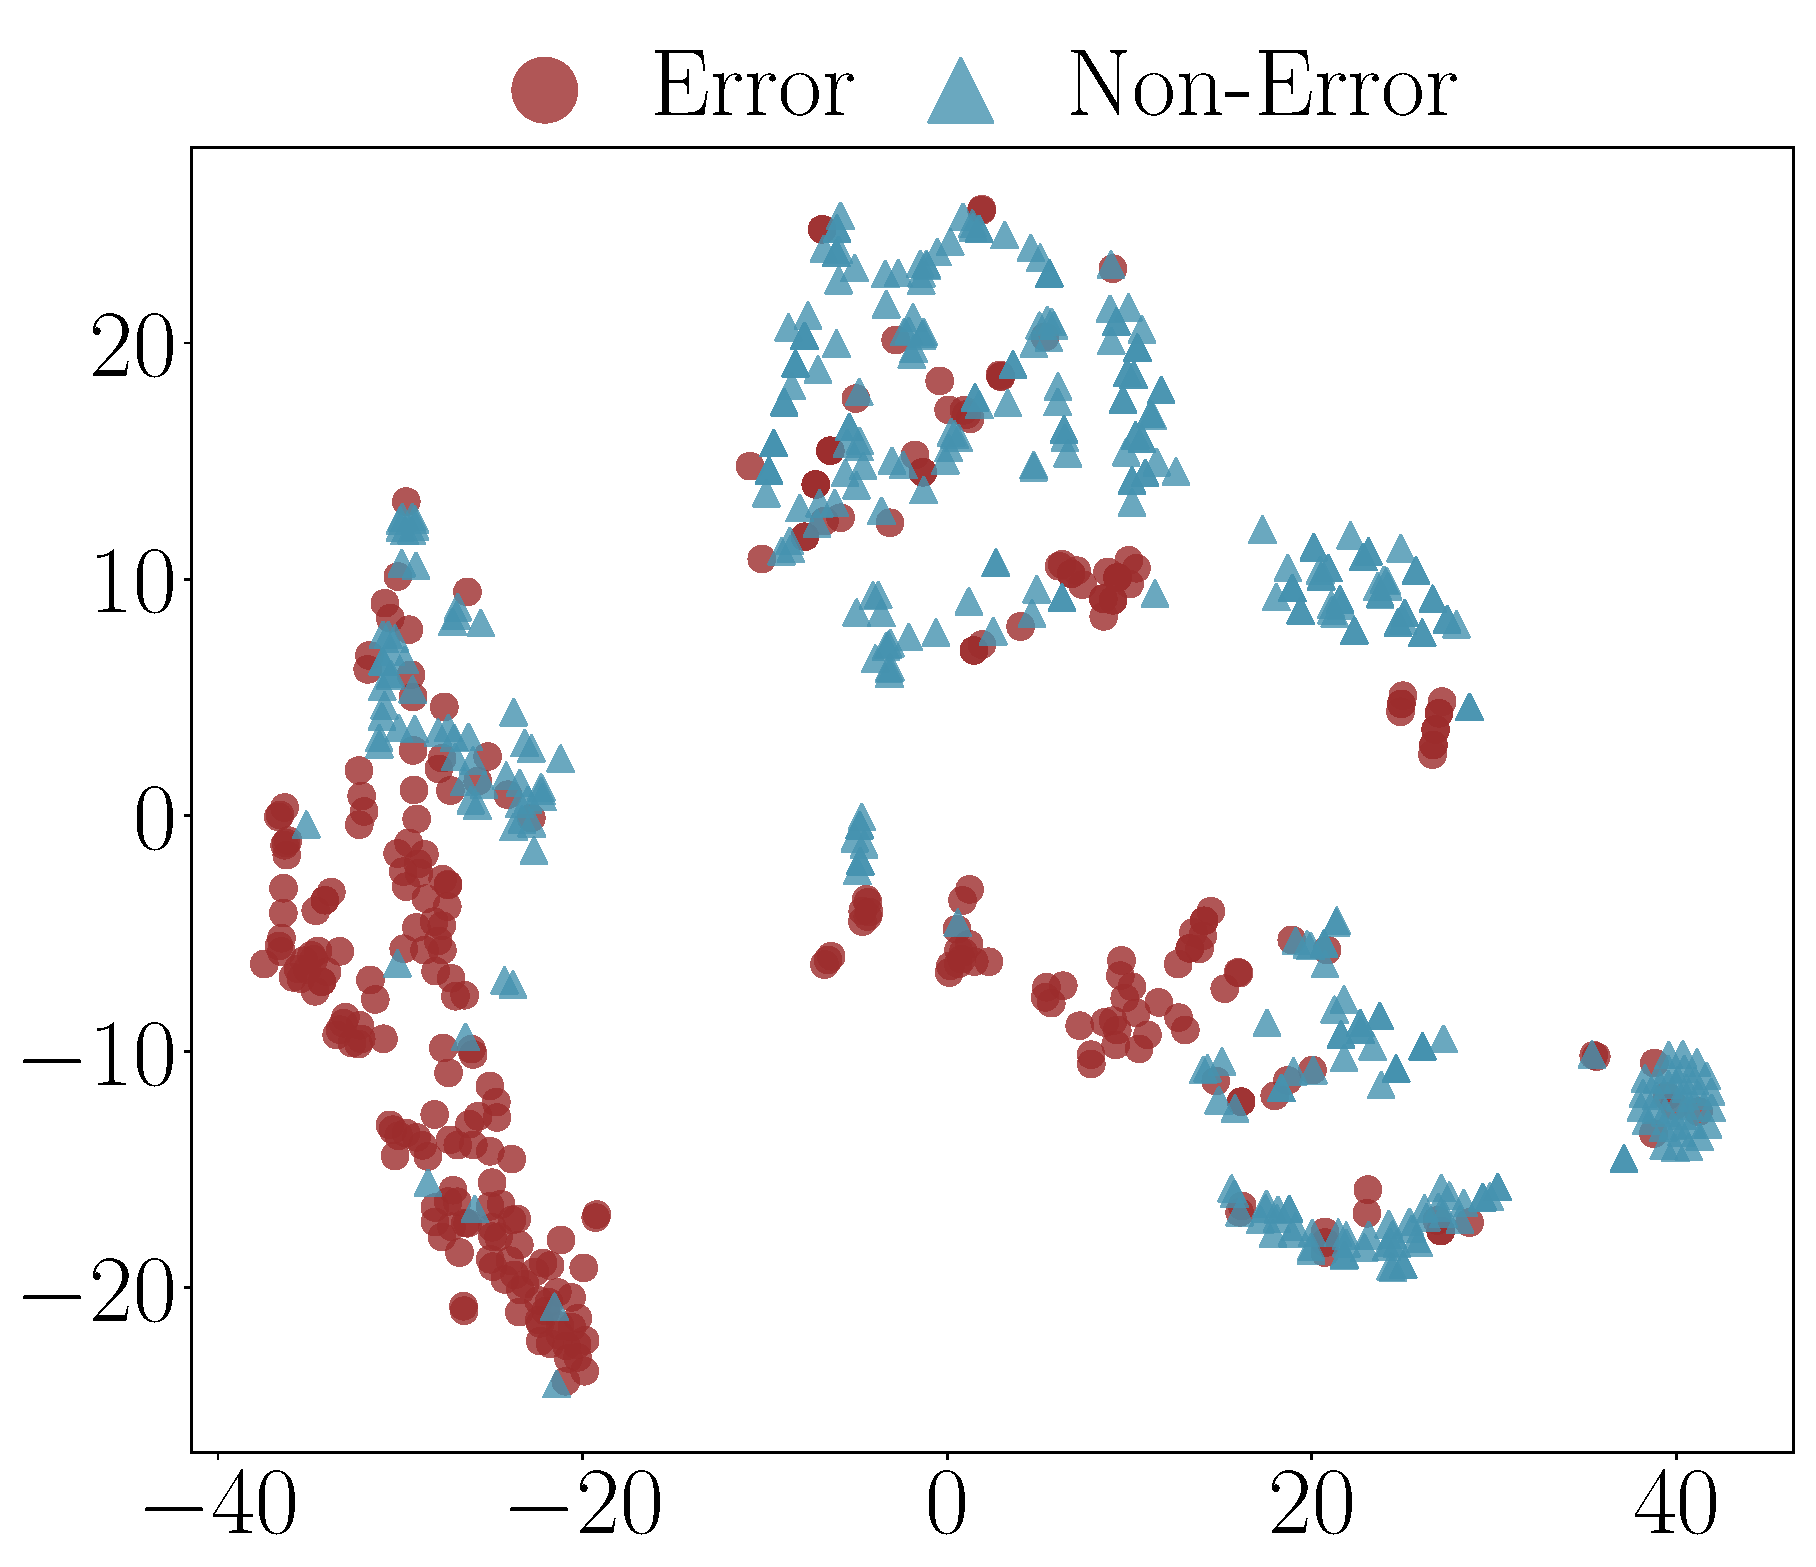
\includegraphics[width=.85\linewidth]{images/glibc_uni_feats.pdf}
    \caption{libc}
     \label{fig:distri3:libc}
\end{subfigure}%
\hfill
\begin{subfigure}[b]{0.5\textwidth}
	\centering
    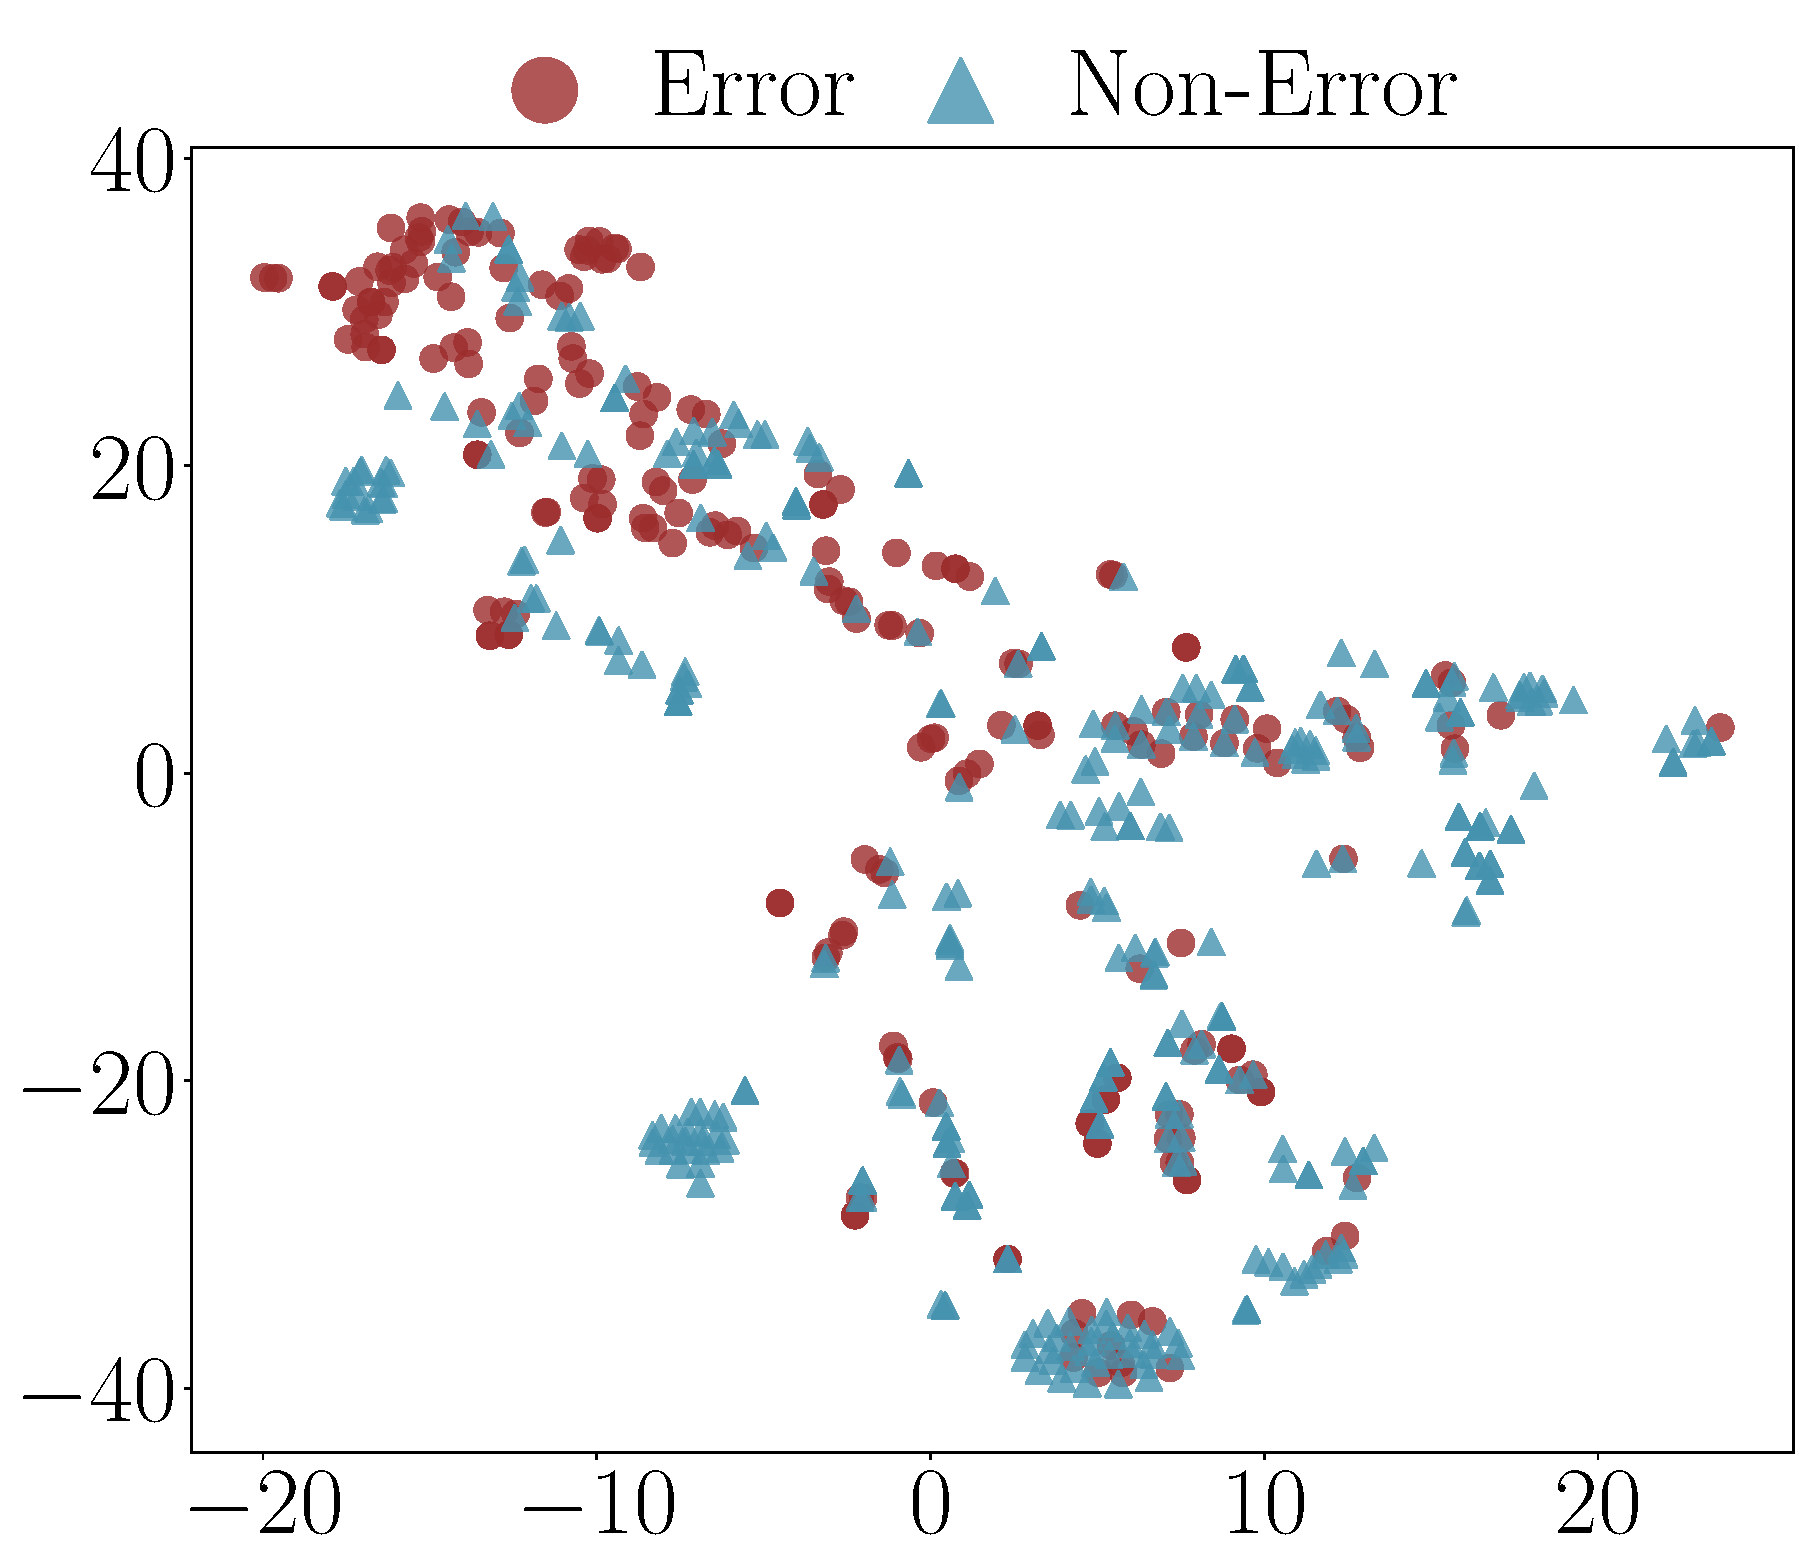
\includegraphics[width=.85\linewidth]{images/kernel_fs_uni_feats.pdf}
    \caption{Linux}
    \label{fig:distri3:linux}
\end{subfigure}
\caption[t-SNE visualization of path distributions in libc and Linux]{t-SNE visualization of path distributions based on universal features in libc and Linux.
The path distribution of libc is quite different from that of Linux.}
\label{fig:distri3}
\end{figure}

The goal of \phasef\ learning is to construct the learned training set (LTS) for a new project
without manually labeling paths.
%
To this end, we need to learn a model for the new project
and use it to select paths that are most likely to be error or non-error.
%
The naive way to obtain such a model is that
we train a model from a pre-labeled project \DS.
We use $\ps(\vec{X}, \vec{Y})$ to denote the path distribution of \DS.
In Phase I, only universal features are used, 
so $x \in \Rset{d_u}$ where $d_u$ is the number of universal features.
The model learned from \DS\ then is:
%
\begin{align} \label{mls}
\sm
&= \argmax_{\theta} \mathbb{E}_{(x, y) \in \DS}[\ln \prb(y | x, \theta)] \nonumber \\
&= \argmax_{\theta} \sum_{x, y} \ps(x, y) \ln \prb(y | x, \theta).
\end{align}

Unfortunately, the obtained \sm\ may not generalize to the new project,
and thus can not be used to construct LTS.
For example, we trained \sm\ from 473 error and non-error paths in libc
and used it (replacing $\theta^*$ in \eqn\ (\ref{predict}) with \sm)
to classify paths in Linux.
The observed accuracy is only 38.9\%,
indicating we can not use \sm\ to determine if a path is error or non-error.
The reason is that the path distributions of 
libc and Linux are quite different, as shown
in Figure~\ref{fig:distri3}. 
%
As a matter of fact, \sm\ can generalize only to projects 
that have similar underlying path distributions,
which is the assumption held by most machine learning approaches~\cite{murphy2012machine}.

\begin{figure}[t]
\centering
\begin{subfigure}[b]{0.5\textwidth}
\begin{Verbatim}[numbers=left,xleftmargin=6mm,fontsize=\footnotesize,
    commandchars=\\\{\}]
\it{/* libc-2.26/malloc/arena.c */}
static int shrink\_heap (...)
\{
  long new\_size;

  new\_size = (long) h->size - diff; 
  if (new\_size < (long) sizeof(*h))
    return -1;
  ...
\}
\end{Verbatim}
\end{subfigure}%
\hfill
\begin{subfigure}[b]{0.5\textwidth}
\begin{Verbatim}[numbers=left,xleftmargin=6mm,fontsize=\footnotesize,
    commandchars=\\\{\}]
\it{/* Linux-4.4.0/open.c */}
static long do\_sys\_truncate (...)
\{
  unsigned int lookup\_flags = LOOKUP\_FOLLOW;
  struct path path;
  int error;

  if (length < 0)
    return -EINVAL;
  ...
\}
\end{Verbatim}
\end{subfigure}
\caption[An example that two similar paths]
{An example that paths from two different projects share similar characteristics,
such as the path length, the number of if-conditions, and the kind of return value.
Functions \prog{shrink\_heap()} and \prog{do\_sys\_truncate()}
return -1 and \prog{-EINVAL} to represent errors, respectively.
}
\label{fig:transfer}
\end{figure}

\parag{Learn a Core Model.}
%
Although directly applying \sm\ to perform path predictions in a new
project does not work, 
it is possible that we can utilize some knowledge from 
the pre-labeled project to help label the paths in the new project.
%
To illustrate, consider the functions
\prog{shrink\_heap()} and \prog{do\_sys\_truncate()}
in Figure~\ref{fig:transfer}. 
%
The two functions are 
syntactically quite different. For example, they differ
in variable names, called functions, and if-conditions.
However, some of their paths are quite similar in terms of 
universal features.
%
For instance,
the universal feature vectors (Section~\ref{sec:app:features:uni})
%, 
%which store the values of universal features as described in Section~\ref{sec:features:uni},
for the error paths in \prog{shrink\_heap()} and \prog{do\_sys\_truncate()} are 
$[0.44, 0.25, 0, 0.33, 0.28, 1, 2]$ and
$[0.50, 0.25, 0, 0.33, 0.33, 0, 2]$,
respectively.
%
We observe that for each single feature, the feature values in
two feature vectors are very close. 
This indicates that the two paths have a similar structure,
such as the path lengths are relatively small,
the numbers of statements before \prog{return} are also small,
and the return expressions are both negative constants. 

The above observation suggests that there 
exist some paths that have similar structures in both the pre-labeled 
and new project,
i.e., the path distributions of the two projects are overlapped.
If we learn a model based on the overlapped path distribution,
then the learned model can be generalized to the new project.
%
This idea is known as reweighting in transfer learning,
which means that we assign higher weights to the overlapped paths
in the pre-labeled project for training a model that can be used in the new project.
In particular, we reweight the likelihood of each path in \DS\ by:
%
\begin{align} \label{mltrans}
\cm
= \argmax_{\theta} \mathbb{E}_{(x, y) \in \DS}[\beta(x, y) \ln \pr (y | x, \theta)],
\end{align}
%
where $\beta(x, y) = \pt (x, y) / \ps (x, y)$,
and $\pt(x, y)$ denotes the path distribution of the new project.
We will discuss how to determine the reweighting factor $\beta(x, y)$ later.

We call \cm\ a core model and have the following property of the obtained core model.
%
%The theorem below indicates that the core model generalizes 
%to the new project. 
\begin{theorem} \label{mlgen}
%Given $\beta(x, y)$, we can thus learn a model with respect to $\DT$ using $\DS$.
%The core model \cm\ learned from the reweighted $\DS$ is equivalent to
%the desired model \tm\ for $\DT$.
The core model \cm\ learned from the reweighted $\DS$ can be generalized to the new project.
\end{theorem}
%

\begin{proof}[Proof of Theorem~\ref{mlgen}]
%
%\vspace{0.1pt}

Let $l(x, y, \theta)$ denote the log-likelihood function $\ln \prb (y | x, \theta)$, we have:
%
\begin{align} \label{mlproof}
\mathbb{E}_{(x, y) \in \DS}[\beta(x, y) l(x, y, \theta)] 
&= \sum_{x, y} \beta(x, y) \ps (x, y) l(x, y, \theta) \nonumber \\
&= \sum_{x, y} \frac{\pt (x, y)}{\ps (x, y)} \ps (x, y) l(x, y, \theta) \nonumber \\
&= \sum_{x, y} \pt (x, y) l(x, y, \theta)
= \mathbb{E}_{(x, y) \in \DT}[l(x, y, \theta)].
\end{align}
%
The right-hand side ($\mathbb{E}_{(x, y) \in \DT}[l(x, y, \theta)]$) is the expected term that we 
want to maximize to obtain the ideal model generalizing to the new project.
However, we can not directly achieve that since we do not have the label information in \DT.
%
Instead, we are able to obtain an equivalent model that also generalizes to the new project
by maximizing the left-hand side ($\mathbb{E}_{(x, y) \in \DS}[\beta(x, y) l(x, y, \theta)]$),
as long as we estimate $\beta(x, y)$.

\end{proof}


Theorem~\ref{mlgen} shows that if we change the path distribution of $\DS$
from $\ps (\vec{X}, \vec{Y})$ to $\beta(\vec{X}, \vec{Y}) \ps (\vec{X}, \vec{Y})$,
we will obtain the core model with good generalizability.
%
The question is how to compute $\beta(\vec{X}, \vec{Y})$?
%
Note that our application scenario is similar to sample selection bias~\cite{zadrozny2004learning} 
and covariate shift~\cite{shimodaira2000improving},
which tackle the problem of training and testing data that are drawn from different distributions.
For example, in our case, we can consider the paths in libc as the training data
and those in Linux as the testing data.
%
Therefore, we follow the same way used in sample selection bias and covariate shift
to approximate $\beta(\vec{X}, \vec{Y})$ via $\pt (\vec{X}) / \ps (\vec{X})$,
where $\pt (\vec{X})$ and $\ps (\vec{X})$ are the marginal distributions of paths 
in the new project and the pre-labeled project, respectively.
Accordingly, we obtain \cm\ using $\DS$ by:
%
\begin{equation} \label{mltrane}
\cm 
= \argmax_{\theta} \mathbb{E}_{(x, y) \in \DS}[\frac{\pt (x)}{\ps (x)} \ln \pr (y | x, \theta)].
\end{equation}

%We find that \eqn~(\ref{mltrane}) intuitively makes sense
The intuition behind equation~(\ref{mltrane}) is that,
given a path $x$ from $\DS$,
a higher weight is assigned to $x$ if it is over-represented in $\DT$,
whereas a lower weight is assigned if $x$ is under-represented in $\DT$.
%
For example, 
if a path in libc has a similar structure as some path in Linux,
then we should focus more on this path with a large weight when training \cm.
On the other hand, if the structure of a path in libc is unlikely to exist in Linux,
then we should ignore this path during training.
%On the other hand, if the representation of a path in libc is unlikely to exist in Linux,
%then we should ignore this path during training.
%
There are various ways to estimate $\pt (x) / \ps (x)$
\cite{zadrozny2004learning,huang2007correcting,sugiyama2008direct}.
In the implementation, we apply the method proposed by \cite{huang2007correcting}
since it can work well even when the sizes of $\DS$ and $\DT$ are small.
%and even when $\ps (\vec{Y} | \vec{X}) \neq \pt (\vec{Y} | \vec{X})$.


%We reuse the paths in Section~\ref{sec:features:valid} 
We reuse the data in Section~\ref{sec:app:features:valid} 
to verify the effectiveness of learning \cm.
Specifically, we consider the labeled paths of libc as $\DS$
based on which the core model \cm\ for Linux could be obtained.
%and Linux were obtained.
We also train \sm\ from libc and compare it with \cm.
We find that
%for both httpd and Linux, 
\cm\ yields better prediction accuracy than \sm\ does on Linux.
%
For example, the accuracy is 38.9\% when directly applying \sm\ to Linux,
while it increases to 73.6\% when using \cm.
%
Thus, with the knowledge transferred from $\DS$,
we can effectively learn \cm\ on different projects.

\parag{Construct LTS.}
%
The obtained \cm\ generalizes to the new project,
but it may not yet achieve very high prediction accuracy.
For example, the accuracy on Linux is 73.6\% only.
This is because either the estimation of $\beta(x, y)$ is not 100\% correct
or \DS\ is not representative enough, or both.
More concretely, since the structures of some error/non-error paths 
in the new project could be unseen in \DS, \cm\ may make wrong predictions on those paths.
%
Nevertheless, we can use \cm\ to sample a set of error and non-error paths
with high confidence as the learned training set $\DO$.

Let \DT\ denote the paths in the new project.
The core model \cm\ computes the probability that
$x \in \DT$ is an error path by $\prb (y = -1 | x, \cm)$, 
or a non-error path by $\prb (y = 1 | x, \cm)$.
The larger the probability, the more accurate the prediction made by \cm.
%
Therefore, we choose paths
for which \cm\ predicts with confidence higher than a threshold $\gamma$
as $\DO$.
In the implementation we set $\gamma$ to 0.85, a relatively high value,
such that $\DO$ is accurate\footnote{
We define the accuracy of the training set
as the ratio between correctly sampled paths and all sampled paths.}.
%
\begin{equation} \label{mllabel}
\DO = \{(x, y) | x \in \DT \land \exists y \in \{-1, 1\}: \prb (y | x, \cm) \ge \gamma \}.
\end{equation}

\begin{figure}[t]
\centering
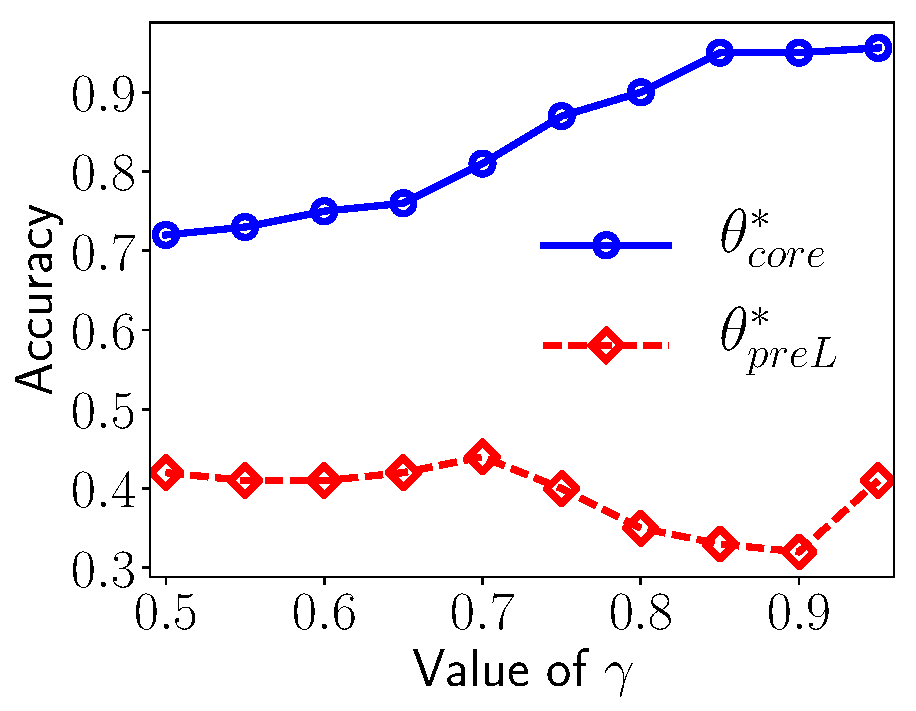
\includegraphics[width=.5\linewidth]{images/dt.pdf}
\caption{LTS accuracy comparison.}
%yielded by \cm\ and \sm.}
%The F-measure of each project changes within $\pm$0.02 of its average.}
\label{fig:trainset}
\end{figure}

We want to emphasize that, at the first glance, one may think of
using \sm\ instead of \cm\ to learn the training set $\DO$,
but it will not work in practice.
%
This is because correctly predicting a path in $\DT$ as error or non-error
%a path in $\DT$ is correctly predicted as error or non-error
is related to the generalizability of the model $\theta^*$.
%that used to predict it.
If the relationship between paths $\vec{X}$ and labels $\vec{Y}$  
in $\DT$ is inappropriately captured by $\theta^*$,
then the computed probability could not represent the confidence
in terms of the ground truth of the predicted path.
%%Therefore, using $\theta_S^*$ that does not generalize to $\DT$ 
%%for constructing $\DO$ leads to poor training set accuracy.
%
For example, we applied \sm, which is learned from libc, 
and \cm, which is learned from the knowledge transferred from libc,
on Linux to construct different $\DO$ 
and compared the training set accuracy in Figure~\ref{fig:trainset}.
We observe that, as the value of $\gamma$ increases from 0.5 to 0.95,
the accuracy yielded by \cm\ monotonically increases from 0.71 to 0.96,
while the accuracy yielded by \sm\ changes arbitrarily.
%
This means that, to learn an accurate training set,
we need to use the core model \cm\ that generalizes to $\DT$.

\subsection{Project-specific Learning (Phase II)}
\label{sec:app:learning:phase2}

Once the learned training set is obtained,
we can extract $d_p$ project-specific features of the new project,
as described in Section~\ref{sec:app:features:pp}.
These features are domain-specific knowledge,
and thus they can be used to represent the structures of error/non-error paths in a finer granularity.
%
Such finer representations are helpful to distinguish error paths from non-error paths.
Therefore, in this phase, we use universal and project-specific features together to 
learn a project-specific model.
Then, we apply the project-specific model on the new project
to classify paths as error or non-error.

\parag{Learn a Per-Project Model.}
%
In Phase II, we use project-specific features together with universal features,
and thus $x \in \Rset{d_u + d_p}$ for any path $x$ in $\DT$.
%
Similar to the way of training a model in supervised learning,
the per-project model \ppm\ trained from $\DO$ is:
%
\begin{equation} \label{mlphase2}
\ppm
= \argmax_{\theta} \mathbb{E}_{(x, y) \in \DO}[\ln \prb (y | x, \theta)].
\end{equation}

Alternatively, we could use other traditional machine learning methods like random forests~\cite{breiman2001random}
to learn \ppm, which might further improve the classification accuracy.
We do not consider, however, deep learning algorithms using neural networks here for two reasons.
First, they require a large amount of training data 
while the size of $\DO$ could be relatively small.
Second, the training process of neural networks usually needs to manually tune the hyper-parameters,
hindering us from automating the error specification generation.
%
To keep our two-phase learning algorithm simple and efficient,
we obtain \ppm\ by solving \eqn\ (\ref{mlphase2}).

\parag{Classify Paths.}
%
Having obtained the per-project model \ppm,
we use it to classify the paths in \DT\ into error or non-error
according to \eqn~(\ref{predict}).
%
It is possible that in the classification result 
all paths in one function belong to the same class.
This does not necessarily mean that the path prediction is wrong
since in practice some functions are infallible.
For example, the function \prog{shmem\_getattr()} in Linux memory management module
will never fail to get the shared memory state.
In our evaluation, we find that about 8\% of the functions are infallible.

\parag{Time complexity of two-phase learning.}
%
We present the details of two-phase learning in Algorithm~\ref{alg:learning}.
%
The time complexity of each step of the algorithm is summarized as follows.
Step 2 uses all the paths in $\DS$ and $\DT$, yielding a time complexity of $O(|\DS \cup \DT|^2)$.
Equations~(\ref{mltrane}) and~(\ref{mlphase2}) in steps 3 and 6 can be solved by using SGD~\cite{robbins1951stochastic},
which take $O(|\DS|)$ and $O(|\DO|)$, respectively.
Steps 4, 5 and 7 have the same time complexity, and all can be finished in $O(|\DT|)$. The overall time complexity is thus 
$O(|\DS \cup \DT|^2 + |\DS| + |\DO| + 3|\DT|) = O(|\DS \cup \DT|^2)$.

\newcommand*{\argmaxl}{\argmax\limits}
\begin{algorithm}[t]
\SetKwInput{Init}{Initialize}
\SetKwInput{Out}{Output}
\SetKwInput{In}{Input}
\Init{Pre-labeled project $\DS$}
\In{New project $\DT$}
\Out{Path prediction $\hat{\vec{Y}}$ for $\DT$}
$\hat{\vec{Y}} \gets \emptyset$\;
\tcp{Phase I}
Estimate $\frac{\pt (x)}{\ps (x)}$ for each path $x$ in $\DS \cup \DT$\;
Train the core model \cm\ using \eqn\ (\ref{mltrane})\;
%Construct the learned training set $\DO$ by selecting the paths in $\DT$ that \cm\ predicts as error or non-error with high confidence\;
Construct the learned training set $\DO$ using \eqn (\ref{mllabel})\;
\tcp{Phase II}
Extract project-specific features from the paths in $\DO$\;
Train the per-project model \ppm\ using \eqn (\ref{mlphase2})\;
\ForEach{$x \in \DT$}{
$\hat{\vec{Y}} \gets \hat{\vec{Y}} \cup \{(x, \argmaxl_{y \in \{-1, +1\}} \prb (y | x, \ppm))\}$\;
}
\Return $\hat{\vec{Y}}$\;
\caption{Two-phase Learning}
\label{alg:learning}
\end{algorithm}

\section{Implementation}
\label{sec:app:impl}

Our implementation mainly consists of extracting paths from source code, 
implementing the two-phase learning (Section~\ref{sec:app:learning}),
labeling initial paths, and collecting error specifications. 
%
Overall, \newTool\ is implemented in 2.2K lines of Python code.

Extracting paths itself includes several steps. First, 
we apply the default project configuration to preprocess the code base 
of each project with GCC using options ``-E -fdirectives-only''.
At this step, GCC will handle the directives such as \prog{\#ifdef}
and \prog{\#define} 
by including appropriate code regions (enclosed by, for example, 
\prog{\#ifdef} and \prog{\#endif}) into the preprocessed code. 
It does not expand macros, allowing us to obtain
information about macros during feature extraction. 
%
%By doing this, the directives such as \prog{\#ifdef} are handled,
%but other operations such as macro expansion are not performed.
%
Next, we apply Joern~\cite{yamaguchi2014modeling} 
%to the preprocessed code 
to build the control-flow and data-dependency graphs of functions, 
and store them in the graph database Neo4j~\cite{neo4j}. 
%
After that, we query the Neo4j database to extract 
paths without duplicate nodes. 
%
Finally, we generate path features and store them 
in MongoDB~\cite{mongoDB}.

%
To solve the optimization problems in two-phase learning,
we adopt SGD solver from the scikit-learn Python package~\cite{scikit-learn}.
%
We initialize \newTool\ by
randomly selecting 100 functions from GNU Tar project (as
the pre-labeled project $\DS$).
There are in total 513 paths of these functions.
We manually label all the paths,
and store the information including 
path features and the corresponding labels in MongoDB.


Given the error paths and non-error paths for a function, its
error specification consists of two parts: the set of return values of error paths 
and the union of error specifications
of functions returned in non-error paths. 
For example, if function \prog{f()} returns \prog{g()} in a 
non-error path, then the error specification of \prog{g()} becomes 
part of that of \prog{f()}. 
%
For each function, we first construct a transitive closure to capture all
its dependencies by
using static analysis of the given code base and system configuration information~\cite{arnold1996software}.
Then, based on the data dependence graph generated by Joern, 
we collect the error specification by implementing a method similar to constant folding~\cite{muchnick1997advanced} 
for evaluating the error return values of each path.
%
Note that, in principle, statically determining function return values
is undecidable.
However, the error values are very often literals,
and thus our approach can effectively collect error specifications for most realistic programs.

When the return expression 
contains function calls, error specification collection
does not work well in two cases. 
%
(1) The source
code of the called function is unavailable, such as a third-party
API that exposes only its type. 
%
We could address this case 
by obtaining the error specifications for these functions from other sources, such
as API documentations.
%
%Second, in our implementation, 
(2) In each particular context,
it might be possible that only a subset of the 
error specification of the callee will become that
of the caller
while our implementation includes the full set
as the error values are collected from all error paths. 
%
%
Nevertheless, we feel this treatment is acceptable for
two reasons. First, our result may be over approximating but never
misses error codes. Second, even over-approximated, 
the error specifications from \newTool\ are small. 
For example, we have measured
their sizes (the number of values in a specification), 
and we find that they are single values in 66\% of cases
and have more than two values in only 10\% of cases. 

While error values are often returned directly from
functions in C code, they can be returned in more complex
ways, such as assigned to some struct field or a parameter
pointer. Our approach, as well as 
other work on error specification generation such as
APEx~\cite{Kang:2016:AAI:2970276.2970354},
currently do not handle such cases.
%
To address this problem,
we can reuse our work on classifying paths,
and extend the step of collecting error specifications
to identify the assignments to fields or
parameter pointers that store error values.
%
However, there is no clear solution to identify such assignments. 
One possible idea is still using machine learning based on features such
as how often or when the fields or parameter pointers are assigned.
We leave this investigation to future work. 

\section{Evaluation}
\label{sec:app:eval}

We use 10 projects (6 libraries 
and 4 applications) to evaluate \newTool.
We provide the details of these study subjects in Section~\ref{sec:app:eval:subjects}.
%In Section~\ref{sec:truth}, we show how the ground truths of error specifications are obtained.
%\newTool\ first predicts error paths,
%and then generates error specifications based on the prediction result.
In Section~\ref{sec:app:eval:phase1}, we present the results of automatically learned training sets for the evaluated projects.
In Section~\ref{sec:app:eval:phase2}, we show the results of error path prediction of \newTool.
%which is also the overall error path prediction accuracy
%of \newTool.
In Section~\ref{sec:app:eval:sepc}, we compare the error specification results of \newTool\ with APEx, a
state-of-the-art error specification generation approach.
In Section~\ref{sec:app:eval:impact}, we discuss the usefulness of project-specific features for error path prediction.
%which serve an important role in the second learning phase.
In Section~\ref{sec:app:eval:performance}, we evaluate the runtime aspect of \newTool.

\subsection{Study Subjects}
\label{sec:app:eval:subjects}

\begin{figure}[t]
\centering
\begin{tabular}{c l | c | c | c | c | c | c }
\toprule
%ID &  Message information contained in the category \\
& & Funcs & Paths  & Path len* & Func calls* & Err range & NErr range \\
\midrule
\multirow{6}{*}{Libs} 
& zlib & 159 & 1001 & 30.40 (\stdf{36.84}) & 2.27 (\stdf{2.53}) & $\errv$ $\le$ 0 &  $\errv$ $\ge$ 0 \\
& Libgcrypt & 500 & 1740 & 21.37 (\stdf{13.73}) & 2.68 (\stdf{2.28}) & $\errv$ = -1 or $\errv$ $\ge$ 0  & $\errv$ $\ge$ 0 \\
& OpenSSL & 129 & 824 & 25.70 (\stdf{15.37}) & 6.97 (\stdf{4.74}) & $\errv$ $\le$ 0  & $\errv$ > 0 \\
& GTK+ & 141 & 429 & 15.49 (\stdf{16.83}) & 3.72 (\stdf{3.19}) & $\errv$ < 0 & $\errv$ $\ge$ 0 \\
& libc & 500 & 2432 & 45.82 (\stdf{30.25}) & 9.14 (\stdf{5.11}) & $\errv$ = -1 or $\errv$ > 0  & $\errv$ $\ge$ 0 \\
& GnuTLS & 260 & 1352 & 14.43 (\stdf{9.59}) & 3.96 (\stdf{3.36}) & $\errv$ $\le$ 0  & $\errv$ $\ge$ 0 \\
\midrule
\multirow{4}{*}{Apps}
& Linux & 1000 & 6245 & 30.16 (\stdf{20.15}) & 6.89 (\stdf{7.52}) & $\errv$ $\le$ 0  & $\errv$ $\ge$ 0\\
& httpd & 500 & 2421 & 36.04 (\stdf{31.56}) & 7.12 (\stdf{9.41}) & $\errv$ = -1 or $\errv$ > 0  & $\errv$ $\ge$ 0\\
& VLC & 102 & 572 & 25.96 (\stdf{16.98}) & 7.51 (\stdf{5.13}) & $\errv$ $\le$ 0  & $\errv$ $\ge$ 0\\
& wget & 154 & 734 & 22.54 (\stdf{12.36}) & 4.09 (\stdf{3.47}) & $\errv$ < 0 & $\errv$ $\ge$ 0\\
\midrule
\multicolumn{2}{c|}{Overall} & 3,445 & 17,750 & 29.20 (\stdf{25.73}) & 6.16 (\stdf{5.94}) & All values &  $\errv$ $\ge$ 0 \\
\bottomrule
\end{tabular}
\caption[Study subjects for \newTool]{Study subjects.
We randomly selected functions from each study subject.
For each function, we evaluated all its paths.
%We treat the C library macros \prog{NULL} and \prog{false} as negative values
%and \prog{true} as positive value.
The values in ``Funcs'' and ``Paths'' columns represent the number of evaluated functions and paths
in each project, respectively.
The columns marked with an asterisk include
average value and the corresponding standard deviation (in bold italic).
We use the short names Err and NErr for Error and Non-Error, respectively.
}
\label{fig:evalsubjects}
\end{figure}

We give the details of the 10 study subjects in Figure~\ref{fig:evalsubjects}.
%
For each project, we randomly selected functions and evaluated all the paths of each function.
We manually investigated the evaluation results to determine the correctness of path prediction and error specification.

Libraries include zlib (v1.2.11), Libgcrypt (v1.8.1), OpenSSL (v1.1.1),
GTK+ (v3.22), libc (v2.26), and GnuTLS (v3.5). 
These libraries expose popular functionalities that are commonly used
by other projects.
%
Existing approaches like APEx can generate error specifications for APIs,
but fail to work for internal functions that implement underlying facilities
since internal functions have a limited number of call sites.
%
\newTool\ does not suffer from this issue, and our evaluation considers both 
APIs and internal functions.

Applications include 
Linux (v4.4.0), httpd (v2.4.29), VLC (v2.1.4), and wget (v1.19).
They are all widely used in reality.
%
Although the functions in applications are usually internal,
\newTool\ is able to infer error specifications for them 
based on their source code.

%TODO maybe we could show that the distributions of path len and func calls are heavy-tail?
Our study subjects are representative 
%of C projects
since the average path length and the number of function calls in each path
vary significantly across projects.
For example, on average, the path length in GnuTLS
is 14.43, while that in libc is 45.82. 
This indicates that projects have very different 
code structures.
Moreover, within a single project, the standard 
deviations of path lengths and function calls are large,
meaning that paths in individual project have diverse structures. 

The last two columns of Figure~\ref{fig:evalsubjects} list
the error range and non-error range for each project. From them,
we make the following observations. 
%
First, error ranges vary across projects.
%different
%projects use different error ranges. 
For example, while zlib uses $\leq 0$ to represent error ranges,
httpd mostly uses values $> 0$ to denote errors. 


Second, in three projects, the error range
and non-error range are overlapping. 
%in many projects, as shown in Figure~\ref{fig:evalsubjects}.
For example, in httpd, the
function \prog{ap\_parse\_from\_data} returns \prog{HTTP\_BAD\_REQUEST},
which is defined to be 400, as an error value. In contrast,
the function \prog{ftp\_set\_TYPE} returns \prog{HTTP\_OK},
a positive value indicating the ftp command is correct, as a non-error value.
As a result, positive values can represent 
both errors and non-errors in this application.
%
In addition,  in five projects, such as zlib, 
0 is used to indicate both error and non-error.
Such counter intuitions suggest that
generating precise error specifications for 
%the functions in 
our study subjects is nontrivial.

\subsection{Learned Training Set Accuracy}
\label{sec:app:eval:phase1}

An obstacle of applying supervised machine learning is that
manually building a training set is 
time-consuming and error-prone~\cite{Sheng:2008:GLI:1401890.1401965}. 
%
To address this issue,
\newTool\ automatically learns the training set by sampling a set of error and non-error paths.
%samples a set of error and non-error paths as the training set.
%such that these paths can be used as the training set in the second learning phase.
%
To measure the accuracy of the learned training set,
we use the sampling precision as the metric,
which is a division of the number 
of correctly sampled error and non-error paths over all sampled paths. 


As Figure~\ref{tab:evallabeling} shows,
the precision of the learned training set for each project is higher than 90\%.
In addition, the average precision of the paths sampled by \newTool\ is high,
about 94\%, meaning that the quality of the learned training set is good.
%
Although there are about 6\% of paths in the learned training set are labeled incorrectly,
they can be considered as noise,
which could be absorbed in phase II
when learning the per-project model for error path prediction.
%
%We also observe that the precision of the learned training set for each project is higher than 90\%.

To check if initializing \newTool\ with different pre-labeled paths affects the precision of learned training sets,
we have repeated the evaluation process by labeling paths from other projects.
We observe that the results are stable across different sets of pre-labeled paths.
For example, the average precision is always higher than 90\%.
%
This supports Theorem~\ref{mlgen} that
the core model obtained in phase I can generalize to different projects,
for the purpose of constructing the learned training set.
%

\begin{figure}[t]
\centering
\begin{tabular}{l | c | c | c |c |c|c|c|c|c|c}
\toprule
%ID &  Message information contained in the category \\
%& zlib & httpd & VLC & OpenSSL & wget & GTK+ & libc & Linux & GnuTLS & Libgcrypt \\
& zlib & httpd & VLC & SSL & wget & GTK+ & libc & Linux & TLS & gcrypt \\
\midrule
%\# of labeled path & 612 & 166 & 273 & 225 & 293 & 122 & 41 & 238 & 120 & 137 & 2,237 \\
%Labeled paths & 0.678 & 0.282 & 0.556 & 0.312 & 0.472 & 0.368 & 0.057 & 0.319 & 0.127 & 0.226 \\
Accu. & 0.957 & 0.920 & 0.965 & 0.955 & 0.952 & 0.953 & 0.950 & 0.944 & 0.942 & 0.958 \\
\bottomrule
\end{tabular}
\caption[Accuracy of LTS for each project]{Accuracy of the learned training set for each project.
The overall precision is 94.6\%.
To save space, we use the short names SSL, TLS, and gcrypt for
OpenSSL, GnuTLS, and Libgcrypt, respectively.}
\label{tab:evallabeling}
\end{figure}

\subsection{Error Path Prediction Accuracy}
\label{sec:app:eval:phase2}

\newTool\ predicts error paths in all analyzed paths based on the classification result 
of project-specific learning.
In this section, we evaluate the error path prediction of \newTool.
%
%In this section, we evaluate the accuracy of error path prediction 
%of project-specific learning, which is also the accuracy of 
%error path prediction of \newTool.
%
Given a set of functions, assume there are $N$ true error paths,
\newTool\ reports $N'$ paths as error paths, and among which 
$N'_t$ are true error paths.
%Denote by $N'_t$ the correctly predicted error paths among $N'$.
We measure the prediction results by using standard metrics precision
(\pr), recall (\re), and \accu\ (\fone), defined as follows.
\[
\it{pr} = \frac{N'_t}{N'} 
\qquad
\it{re} = \frac{N'_t}{N}
\qquad
\it{\fone} = 2 \times \frac{\it{pr} \times \it{re}}{\it{pr} + \it{re}}
\]
%
%In other words,
The precision is the ratio of correctly predicted error paths,
the recall is the ratio of covered true error paths, and the 
\fone\ is the measure of error path prediction accuracy.

Figure~\ref{fig:evalpathm} (the columns under ``With project-specific features'')
shows that, on average, the prediction precision of \newTool\ for all
10 projects is 91.2\% and the recall is 89.1\%. 
%
Note that the F-measures for GnuTLS and Linux are
86.5\% and 85.3\%, respectively,
which are about 5\% lower than the average.
The main reason is that
the paths in the learned \typical\ set of each of the two projects
have similar code structures.
%
Therefore, the training data fed to project-specific learning
is not representative enough, affecting the accuracy of the trained model.
%%making their F-measures not as good as those of the others.
%
Figure~\ref{fig:evalpathm} also shows that the accuracy of error path prediction 
across projects is stable, since
the standard deviation of F-measure is 0.04.

\begin{figure}
\centering
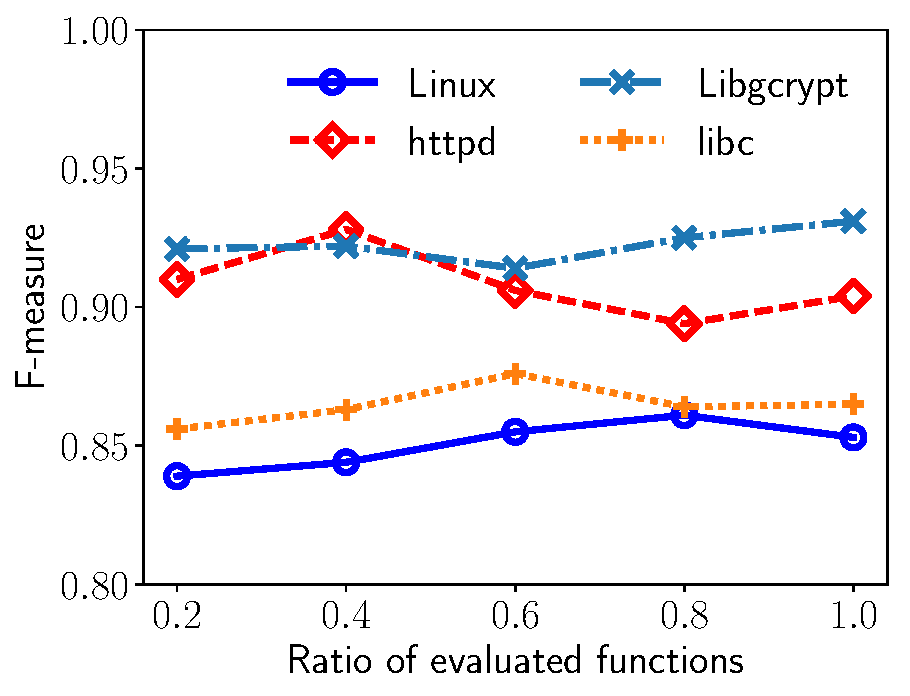
\includegraphics[width=0.65\linewidth]{images/stab.pdf}
\caption{Stability of error path prediction.}
%The F-measure of each project changes within $\pm$0.02 of its average.}
\label{fig:change}
\end{figure}

%
Given the number and sizes of projects used for evaluation, 
it is infeasible to evaluate all functions in each project. 
A question is, how do we make sure that the result is representative?
To address this, we have chosen 4 projects and for each
we gradually investigated more functions and paths and 
assess if the F-measure is stable. For example, for Linux,
we first randomly selected 200 functions, evaluate them, and recorded
the result. We then chose another 200 functions and repeated the process.
We continued until all 1,000 functions were evaluated. 
We also applied the same process
to httpd, Libgcrypt, and libc, but with an interval of 100 functions.
%since some of them do not have 1000 functions. 
We plot the result in Figure~\ref{fig:change}. From the figure, we observe that the evaluation
result is stable within each project. Thus, we are confident that our
results are representative.

\begin{figure}[t]
\centering
\begin{tabularx}{\textwidth}{ c l | Y | Y | Y | Y | Y | Y }
\toprule
\multicolumn{1}{c}{} 
 & \multicolumn{1}{l|}{} 
 & \multicolumn{3}{c|}{With project-specific features}
 & \multicolumn{3}{c}{Without project-specific features} \\
 &  & Precision & Recall & \fone & Precision & Recall & \fone \\
\midrule
\multirow{6}{*}{Libs}
& zlib & 0.947 & 0.974 & 0.960 & 0.792 & 0.974 & 0.873 \\
& Libgcrypt & 0.916 & 0.947 & 0.931 & 0.883 & 0.929 & 0.905 \\
& OpenSSL & 0.983 & 0.961 & 0.971 & 0.915 & 0.961 & 0.937 \\
& GTK+ & 0.818 & 0.991 & 0.896 & 0.581 & 0.991 & 0.732 \\
& libc & 0.821 & 0.962 & 0.886 & 0.644 & 0.950 & 0.768 \\
& GnuTLS & 0.923 & 0.814 & 0.865 &  0.940 & 0.809 & 0.869 \\
\midrule
\multirow{4}{*}{Apps} 
& Linux & 0.952 & 0.773 & 0.853 & 0.814 & 0.791 & 0.802 \\
& httpd & 0.859 & 0.954 & 0.904 & 0.689 & 0.966 & 0.804 \\
& VLC & 0.908 & 0.984 & 0.944 & 0.872 & 0.984 & 0.924 \\
& wget & 0.931 & 0.954 & 0.942 & 0.898 &  0.944 & 0.920 \\
\midrule
\multicolumn{2}{c|}{Overall} & 0.912 & 0.891 & 0.901 & 0.790 & 0.903 & 0.843 \\
\bottomrule
\end{tabularx}
\caption[Results of error path prediction]{Results of error path prediction with/without project-specific features.
The results for ``with project-specific features'' are described in Section~\ref{sec:app:features:uni}
and their difference with those for ``without project-specific features'' are described in Section~\ref{sec:app:features:pp}.}
\label{fig:evalpathm}
\end{figure}

\subsection{Error Specification Accuracy}
\label{sec:app:eval:sepc}

In this section, we measure the inferred error 
specifications of \newTool. We reuse the three metrics defined
in Section~\ref{sec:app:eval:phase2} here but reinterpret 
$N$ as the number of functions that we evaluate about their 
specifications, $N'$ as the number of functions for which
\newTool\ generates specifications, and 
$N_t'$ as the number of functions for which
\newTool\ generates correct specifications. 

In Section~\ref{sec:app:impl},
we discussed that \newTool\ is unable to collect the full 
error specification for function \prog{f} if it uses some
function call \prog{g} as the return expression in a path and the source
code of the callee \prog{g} is unavailable to \newTool. 
%As we discussed
%in Section~\ref{sec:impl}, 
Such limitation is not fundamental to \newTool. 
%For this reason, 
Our evaluation considers two $N$s, one with functions of the form \prog{f} above and one
without. Accordingly, we have two different recalls.
The precision keeps the same no matter which $N$ we use.

\begin{figure}
\centering
\begin{tabularx}{\linewidth}{ c l | Y | Y | Y | Y | Y }
\toprule
\multicolumn{1}{c}{} 
 & \multicolumn{1}{l|}{} 
 & \multicolumn{2}{c|}{Precision}
 & \multicolumn{3}{c}{Recall} \\
 & & \scriptsize \newTool & \scriptsize APEx & \scriptsize \newTool & \scriptsize \newTool* & \scriptsize APEx \\
\midrule
\multirow{5}{*}{Libs}
& zlib & 0.90 & 0.50 & 0.93 & 0.98 & 0.27\\
& Libgcrypt & 0.80 & 0.82 & 0.63 & 0.89 & 0.64\\
& OpenSSL & 1.0 & 0.78 & 0.87 & 0.96 & 0.62 \\
& GTK+ & 0.85 & 0.84 & 0.93 & 1.0 & 0.36 \\
& libc & 0.86 & 0.76 & 0.82 & 0.87 & 0.65  \\
& GnuTLS & 0.94 & 0.74 & 0.65 & 0.92 & 0.34\\
\midrule
\multirow{4}{*}{Apps}
& Linux & 0.97 & N/A & 0.80 & 0.98 & N/A \\
& httpd & 0.81 & N/A & 0.71 & 0.95 & N/A \\
& VLC & 1.0  & N/A & 0.91 & 1.0 & N/A \\
& wget & 0.82 & N/A & 0.86 & 0.96 & N/A  \\
\midrule
\multicolumn{2}{c|}{Overall} & 0.91 & 0.77 & 0.78 & 0.94 & 0.47 \\
\bottomrule
\end{tabularx}
\caption[Results of generated error specifications]{Results of generated error specifications.
The recall values in column ``\newTool*'' are calculated by 
filtering out the cases that lack necessary source code.
The overall \accu\ of \newTool\ and APEx is
0.92 and 0.58, respectively.}
\label{fig:evalcerrspec}
\end{figure}

We present the precision and both recalls in Figure~\ref{fig:evalcerrspec}.
%
%
We observe that the recall values (under ``\newTool'' in the table) 
for Libgcrypt, GnuTLS, and httpd
are much lower than those for other projects.
The reason is that these projects are heavily dependent on third-party libraries
that are not contained in our analyzed source code.
For example,  in libgcrypt that requires the third-party library libgpg-error,
the error path \newTool\ predicted in function \prog{make\_space}
returns \prog{GPG\_ERR\_TOO\_LARGE}. 
However, since the code of libgpg-error was not included,
we missed the error value of \prog{GPG\_ERR\_TOO\_LARGE}
in the error specification.
%We can simply include the header files from 3rd-party libraries, 
%which define the error codes,
%to improve the recall of \newTool.  

In Figure~\ref{fig:evalcerrspec}, we also 
show the error specification results from APEx~\cite{Kang:2016:AAI:2970276.2970354}
for a comparison. 
Since most functions in applications are internal and APEx does not work for them,
we put ``N/A'' for the entries where APEx is not applicable. 
%and the original paper~\cite{Kang:2016:AAI:2970276.2970354} lacks such numbers.
%
We observe that the precision of \newTool\ is much higher than
that of APEx for all projects, except for Libgcrypt, for which 
APEx is 2\% more precise than \newTool. 
For recall, 
%a more important metric,
\newTool\ is about 30\% better than APEx for all projects, 
except for Libgcrypt, for which
\newTool\ and APEx perform similarly. 
If we ignore the functions that lack necessary source code, 
then the recall of \newTool\ 
(under ``\newTool*'' in Figure~\ref{fig:evalcerrspec}) is significantly
higher than that of APEx. For zlib, GTK+, and GnuTLS, the recall of
\newTool\ is triple that of APEx, and for other three projects, \newTool\
is 30\% better. 
%
Overall,
\newTool\ outperforms APEx significantly
in both precision and recall. 



\subsection{Usefulness of Project-specific Features}
\label{sec:app:eval:impact}

\begin{figure}
\centering
\begin{Verbatim}[numbers=left,xleftmargin=6mm,fontsize=\footnotesize,
    commandchars=\\\{\}]
\it{/* Linux-4.4.0/aio.c */}
static struct kioctx *ioctx\_alloc(unsinged nr\_events)
\{
  ...
  err = ioctx\_add\_table(ctx, mm)
  if (err)
    goto err\_cleanup;
  ...
  \correctline{return ctx;}

err\_cleanup:
  ...
  aio\_free\_ring(ctx);
  ...
  \errline{return ERR\_PTR(err);}
\}
\end{Verbatim}
\caption[An example of the usefulness of project-specific features]{An example of project-specific features helps predict error paths.
The line marked red represents an error return,
while the line marked green represents a correct return.}
\label{fig:psfeature-use}
\end{figure}


To improve the error path prediction precision,
a key idea introduced in \newTool\ is to use project-specific features
to better differentiate error paths from non-error paths.
%
In this section, we investigate the usefulness of project-specific 
features for error path prediction.

We repeated the process of evaluating the accuracy of path prediction
without considering the project-specific features.
We compare the results with those with project-specific features
and present the comparison result in Figure~\ref{fig:evalpathm}.
%
We find out that project-specific features improve the overall precision by 
about 12\%, and the precision for GTK+ by 23\%, libc and httpd by 17\%, 
and Linux and zlib by 15\%. 
Meanwhile, the overall recall with project-specific features is 89.1\%,
which is almost the same
as that without project-specific features.
The results mean that, with project-specific features,
\newTool\ discovers most error paths
with fewer false positives (a false positive predicts a non-error path as an error path).
%
Therefore, project-specific 
features are helpful in predicting error paths.


To illustrate how project-specific features help differentiate error paths 
from non-error paths,
we use a concrete example shown in Figure~\ref{fig:psfeature-use}.
%
In this code excerpt,
the error path $p_{\it{err}}$ returning \prog{ERR\_PTR(err)} 
is predicted as a non-error path with universal features only.
%
%is not labeled after the first learning phase,
%and it is predicted as a non-error path in the second learning phase without project-specific features.
The reason is that the universal feature values of this path are quite similar to those of non-error paths in the training data.
%
However, the return expression \prog{ERR\_PTR(err)} and
the function call \prog{aio\_free\_ring()} (at line 13) within the latest conditional before return statement
match the patterns in the extracted project-specific information 
from the learned training set for Linux.
\newTool\ thus successfully classifies $p_{\it{err}}$ as an error path with project-specific features.

\subsection{\newTool\ Performance}
\label{sec:app:eval:performance}

For each project, we measured the time for 
parsing, core-model learning, project-specific learning, 
and error specification generation.
%on CentOS 6.7 with 1 Intel i7-3940xm processor and 16 GB memory.
%Table~\ref{fig:evalhperformance} 
We present the detailed result in Figure~\ref{fig:evalhperformance}.
%of the time consumption of each part in Appendix~\ref{sec:appy}.
Since we use the third-party tool Joern to parse source code, we 
focus our discussion on the time consumed by other parts of \newTool.
%
The average total time to learn error specifications over the 10 
projects is 614.8 seconds,
without the code parsing time.
Compared to APEx,
our tool is much faster.
For example, for GnuTLS, \newTool\ took in total 15 mins to generate 
error specifications for 260 functions,
while APEx took about 50 mins to generate error specifications 
for only 47 functions. 


\begin{figure}[t]
\centering
\begin{tabular}{l | c | c| c| c | c }
\toprule
%ID &  Message information contained in the category \\
& Linux & libc & httpd & GnuTLS & zlib \\
\midrule
Code parsing & 4,112.56 & 1,129.08 & 1,432.90 & 642.13 & 326.46 \\
Learning phase I & 456.95 & 182.44 & 175.83 & 63.73 & 18.94 \\
Learning phase II & 1,903.96 & 430.18 & 421.94 & 195.24 & 134.56 \\
Error spec generation & 3.15 & 2.39 & 2.30 & 1.43 & 1.73 \\
\midrule
Total & 6,476.62 & 1,744.09 & 2,032.97 & 904.05 & 481.69 \\
\bottomrule
\end{tabular}
\caption[Performance of \newTool]{Performance of \newTool\ in seconds.
The runtimes for Linux and zlib are the largest and smallest among all the evaluated projects, respectively,
while those for libc, httpd and GnuTLS are in-between.
The times are measured on CentOS 6.7 with 1 Intel i7-3940xm processor and 16 GB memory.}
\label{fig:evalhperformance}
\end{figure}

The number of paths may grow exponentially as 
the number of if-statements increases.
For example, 
a code block with 20 sequential if-statements
will lead to about $10^7$ paths,
requiring more time to analyze such a large number of paths.
%
This is, however, an inherent problem to all path-sensitive analyses~\cite{Dillig:2008:SCS:1375581.1375615}.
%
To alleviate the path explosion problem,
we perform a random walk on a CFG restricted to extract at most $M$ paths
(we set $M$ to 1024 in our implementation),
which is a common practice in literature~\cite{defreez2018path}.
%
Fortunately, functions with such
large numbers of sequential if-statements are uncommon in practice.


To evaluate the scalability of \newTool,
we applied it on the memory management module of Linux,
which contains 3,629 functions and 25,617 paths.
The whole analysis process was finished in 8 hours, of which
58 mins was used by \newTool\ for learning error specifications and
the rest was used by Joern for parsing the source code.
%and \newTool\ took 58 mins to generate error specifications.
The result shows that \newTool\ could scale to large projects.

\section{An Application: Detecting Incorrect Error Code Assignments}
\label{sec:app:evalbugs}

\begin{figure}[t]
\begin{Verbatim}[numbers=left,xleftmargin=6mm,fontsize=\footnotesize,
    commandchars=\\\{\}]
\it{/* Linux-4.9-rc6/nbd.c */}
static int \_\_init nbd\_init(void)
\{
  ...
  err = blk\_mq\_alloc\_tag\_set(\&nbd\_dev[i].tag\_set);
  if (err) \{
    put\_disk(disk);
    goto out;
  \}

  disk->queue = blk\_mq\_init\_queue(\&nbd\_dev[i].tag\_set);
  if (!disk->queue) \{
    blk\_mq\_free\_tag\_set(\&nbd\_dev[i].tag\_set);
    put\_disk(disk);
    goto out; \errline{//forgot to assign variable \it{err}} \errline{with correct error value.}
  \}
  ...
  return 0;

out:
  ...
  return err;
\}
\end{Verbatim}
\caption[An example of an incorrect error code assignment]{An example of an incorrect error code assignment.
Function \prog{nbd\_init()} returns \prog{0} and negative values to represent success and error, respectively.}
\label{fig:errbug}
\end{figure}

To handle a program failure correctly, a function should return an error code
to inform the upper-level functions.
In practice, however, developers may forget to propagate error values
or the return value with a correct error code gets 
overwritten by a non-failure value due to complicated function logic,
causing error assignment bugs~\cite{gunawi2008eio,liang2016antminer,Tian:2017:ADR}.
For example, in Figure~\ref{fig:errbug}, 
negative values should be propagated upstream when the call to
\prog{blk\_mq\_init\_queue()} at line 11 fails.
However, the developer forgot to set the appropriate value of \prog{err} 
for this failure, and a non-failure value \prog{0} is returned.
This misleads the system into believing that the network block device is initialized successfully, 
even when unexpected events have occurred during the initialization  \prog{nbd\_init()}. 
%

%\newTool\ can effectively detect such error handling bugs based on
%its path prediction results and generated error specifications.
We propose a simple approach \bugTool\ to detect error assignment bugs based on the 
%We can detect error assignment bugs based on the
generated error specifications and path prediction results from \newTool.
%
We illustrate how \bugTool\ works with the example in Figure~\ref{fig:errbug}. 
We represent a path by a sequence of program line numbers $\langle l_i, l_{i+1}, ....l_j \rangle$.
By applying \newTool\ to the source code containing \prog{nbd\_init()},
the path $p_m$ $\langle 2, ....17, 18 \rangle$ is predicted as a non-error path,
and the path $p_n$ $\langle 2, ....12, 13, .... 21, 22 \rangle$ is predicted as an error path.
Intuitively, $p_m$ and $p_n$ should return different values since one is an
error path while the other is not.
%to indicate success and error, respectively.
However, the return values of $p_m$ and $p_n$ both evaluate to 0.
\bugTool\ considers such conflicting situations as incorrect error code assignments. 
In general, \bugTool\ reports a potential error
assignment bug if two paths from a single function are classified into
%\newTool\ classifies two paths from a single function into
different classes  by \newTool\ but return the same value.
%Therefore, such conflicting situations that, within one function,
%\newTool\ classifies two paths returning the same value into different classes
%indicate potential incorrect error code assigning.


\begin{figure}
\centering
\begin{tabular}{l | c | c | c | c }
\toprule
%ID &  Message information contained in the category \\
& \# of Reported & \# of Known  & \# of Unknown & Precision \\
\midrule
Linux & 56 & 45 & 0 & 0.80 \\
httpd & 2 & 0 & 1 & 0.50 \\
VLC &  9 &  3 & 4 & 0.77 \\
zlib &  2 &  0 & 2 & 1.0 \\
OpenSSL & 3 & 0 & 2 & 0.66 \\
\midrule
Total & 72 &  48 & 9 & 0.79 \\
\bottomrule
\end{tabular}
\caption[Results of detecting incorrect error code assignments]{Results of detecting potential incorrect error code assignments.
%The ``Reported'' bugs are those cause conflicting situations in \bugTool\ results.
The ``Known'' bugs are those that have already been fixed by developers. 
The ``Unknown'' bugs are 
those still appear in the tested versions.
%the potential undiscovered bugs after manually inspecting the reported bugs.
}
\label{fig:bugsum}
\end{figure}

We evaluated the effectiveness of detecting error assignment bugs 
of \bugTool\ on five projects,
%we have applied it to five projects, listed in 
listed in Figure~\ref{fig:bugsum}. 
%
For Linux, 
we applied our tool to its memory management module and
49 functions that have already been reported 
to have error assignment bugs in kernel Bugzilla. 
%
We did not apply \bugTool\ to the whole Linux because
it takes Joern too much time to parse the full source
code.
%and it is beyond MongoDB's capacity to store
%all paths.
%
For the rest of the four projects, we applied \bugTool\ to
their full code base. 
%
The program versions used in this testing are the same as
those in Section~\ref{sec:app:eval:subjects}, which are the 
latest release versions, except for Linux and VLC.

Figure~\ref{fig:bugsum} presents the bug detection results of \bugTool.
In total, \bugTool\ reports
72 functions that may contain
error assignment bugs.
We manually inspected all of them and found that 57 functions are
very likely to have real bugs\footnote{\bugTool\ does not find an excessive number of error assignment 
bugs, which coincides with an empirical study performed by 
\cite{Tian:2017:ADR}
%, who finds out 
that error assignment
bugs account for about only 7\% of all error handling bugs.
}. 
Thus, the overall precision of detecting bugs is 79\%.
%
Among the 57 potential bugs, 48 bugs are previously known, including
45 bugs from Linux (\newTool\ detects 45 out of 49 included for testing) 
and 3 from VLC, which have been fixed in a later VLC release. 
The rest of the 9 bugs are previously unknown,
including 1 from httpd, 4 from VLC, 2 from zlib, and
2 from OpenSSL.
%
We have submitted these bugs to the development communities
and are awaiting confirmations.

\bugTool\ reports a potential bug when \newTool\ classifies two paths 
into different classes (error and non-error) but their returned expressions
evaluate to a same value.
%
The false positive rate of \bugTool\
is 21\% as shown in Figure~\ref{fig:bugsum},
which happens for two reasons: 
%
\begin{enumerate*}[label=(\arabic*)]
\item a path is misclassified and
\item a return expression is evaluated incorrectly.
\end{enumerate*}
%
Case (1) happens because the precision of error path prediction
of \newTool\ is not 100\% (Figure~\ref{fig:evalpathm}). 
Case (2) happens because our current
value evaluation of return expression is based on the idea of constant 
folding (Section~\ref{sec:app:impl}), which is not very accurate 
and could be improved by, for example, using LLVM.
%
Since our main goal is to learn precise error specifications
and that in the section is to demonstrate the usefulness of error path
prediction and error specifications, we leave the improvement
of (2) as future work.
%
In addition to detecting error assignment bugs, error 
specifications can be used to detect other error handling bugs.
%
According to~\cite{Tian:2017:ADR}, 
34\% of all error handling bugs are caused by
forgetting to check return values against errors.
%
%One common type of such bugs, accounting for 34\% of all
%error handling bugs according to~\citet{Tian:2017:ADR}, 
%forgets to check return values against errors. 
%
Such bugs can be detected if function return values are not
checked against all values in the function's error specification.
%
We plan to develop a tool for detecting missing error checks in the future.



\chapter{Conclusion}
\label{sec:conclusion}

This dissertation presents my work on type error debugging and 
the machine learning-based solution to improve error debugging.
To summarize, this work makes the following contributions.

\begin{enumerate}

\item By manually analyzing 2,757 student ill-typed programs 
and recording the information about how type errors were fixed, 
we derive many interesting observations that inform future directions in designing type error debuggers.
Our results are also beneficial for teachers to better organize course contents in teaching functional programming
and for students to become more effective in fixing type errors.

\item We give a fundamental understanding about the conditions for existing error debuggers to work well.
Our discussion is based on general ideas underlying many debuggers, rather than the behaviors of individual debuggers.
Thus, future debuggers that share similar underlying ideas
should consider how to effective handle type errors that are caused by wrong use of parentheses or brackets and wrong type annotations.

\item We design a set of features to represent type errors,
including three kinds of information from:
(1) the type conflicts, (2) the program structure, and (3) the error message.
We develop an algorithm to compute the differences between two conflicted types,
and the algorithm can be further be employed to design more powerful error ranking heuristics.

\item We develop a machine learning-based debugger \newCompiler\ to learn the relation between the proposed features and the kinds of type errors.
\newCompiler\ could provide informative error messages for nonstructural errors based on the learned relation.
We evaluate \newCompiler\ by comparing it with other leading error debuggers 
and show that our approach can locate nonstructural errors accurately and generate concrete fixes for them.

\item We propose a zero-shot learning approach, \newTool,
to infer precise error specifications directly from program source code.
One of the main innovations is that we introduced a two-phase learning paradigm
that requires minimal labeling efforts from us to initialize \newTool,
while no such efforts from users to use \newTool.
%
Theoretical analysis and evaluation results show that 
this novel learning paradigm enables \newTool\ to generalize to different C projects.
We believe that the same methodology could be easily applied to other specification mining problems.
%
In addition, \newTool\ effectively
extracts and makes use of project-specific information for generating accurate
error specifications, with precision and recall both being more than 90\%. 
%
\newTool\ helps remove a 
main obstacle for broader applications of many error-handling bug
detection tools, which require precise error specifications as an input.
We also use \newTool\ to find 57 error handling bugs in 5 real-world projects.

\end{enumerate}

%\include{chapter11}	

%\include{chapter12}	
%
% Appendix/Appendices
%
% If you have only one appendix, use the command \appendix instead
% of \appendices.
%
\appendix

\section{Kinds of Helium Message}
\label{sec:msgkind}

In Section~\ref{sec:features:feature},
we consider the kind of error messages generated from Helium as a feature to represent type errors.
In this section, I present the message kinds and the corresponding feature values in Figure~\ref{fig:heliummsg}.

\begin{figure}
\centering
\begin{tabular}{l | c }
\toprule
%ID &  Message information contained in the category \\
String contained in the message & Value \\
\midrule
Type error in application. & 1\\
Type error in constructor. & 2\\
Type error in infix application. & 3 \\
Type error in literal.  & 4\\
Type error in right-hand side. & 5 \\
Type error in [variable | enumeration | element of list]. & 6 \\
Type error in guard. & 7 \\
Type error in guarded expression. & 8 \\
Type signature is too general. & 9 \\
Don't know which instance to choose for [Eq | Num]. & 10 \\
Type error in [negation | overaloaded function]. & 11 \\
Type error in [explicitly typed binding | infix pattern application]. & 12 \\
%Type error in [explicitly typed binding | infix pattern application | pattern of function binding]. & 12 \\
Other. & 13 \\
\bottomrule
\end{tabular}
\caption{Values for Feature 1.}
\label{fig:heliummsg}
\end{figure}

%\include{chapter-appendix1}
%\include{chapter-appendix2}
%\include{chapter-appendix3}

%
% Generate the bibliography.
%

%\nocite{*}      % This command causes all items in the               %
                % bibliographic database to be added to              %
                % the bibliography, even if they are not             %
                % explicitly cited in the text.                      %

% Here the bibliography is inserted.
% Replace "example" with the name of your ".bib" file
\bibliography{error-reporting,me,paper,pldi,ml,errspec}                      
\index{Bibliography@\emph{Bibliography}}
%


%
% Generate the index.
% 
%
\printindex     % Include the index here. Comment out this line      
%               % with a percent sign if you do not want an index .  
%

\begin{abstract}
test
\end{abstract}

\end{document}
% The following comment block is used by the different flavors of EMACS and
% the AUCTEX package to manage multiple documents.  In order for AUCTEX
% to understand you're working with multiple files, you should define
% the TeX-master variable as a file local variable that identifies your
% master document.
%
% Please do not remove.
%%% Local Variables: 
%%% mode: latex
%%% TeX-master: "example.tex"
%%% End: 
